\documentclass{article}

% ===== Language switch =====
\newif\ifkorean
% 여기서 언어 선택:
% \koreantrue   % 한글 버전
\koreanfalse    % 영어 버전
% ===========================

% ------------------------ Packages ------------------------
\usepackage{amsmath, amssymb}
\usepackage{tikz}
\usepackage{graphicx}
\usepackage{caption}
\usepackage[margin=1in]{geometry} % 전체 문서: portrait
\usepackage{pdflscape}            % 특정 페이지만 가로(landscape)로
\usetikzlibrary{shapes, arrows, positioning, fit, calc}
\usetikzlibrary{shapes.geometric, arrows.meta, positioning, calc, decorations.pathreplacing}

% 한글일 때만 kotex 로딩 (설치돼 있으면)
\usepackage{kotex}

% Page numbering
\usepackage{fancyhdr}
\pagestyle{fancy}
\fancyhf{}
\fancyfoot[C]{\thepage}
\renewcommand{\headrulewidth}{0pt}

% ------------------------ Document ------------------------
\begin{document}
\ifkorean
  \title{트랜스포머 병렬화: 차원 기반 시각적 가이드\\[0.3em]
         \large A Visual, Dimension-Oriented Guide to Transformer Parallelism}
\else
  \title{A Visual, Dimension-Oriented Guide to\\ Transformer Parallelism}
\fi

\date{November 6, 2025}
\maketitle

\clearpage

\tableofcontents
\listoffigures
% \listoftables

\clearpage

% ==========================================================
% 1. Introduction
% ==========================================================
\ifkorean
  % ==========================================================
% 1. Introduction (Korean)
% ==========================================================
\section{서론}

Transformer와 그 변형 모델들은 현재 대규모 언어 및 비전 모델에서 사실상 표준 아키텍처가 되었다.
최신 시스템들은 수백억에서 수천억 개의 파라미터를 가진 모델을 여러 가속기에 분산시켜 학습하고 서빙하기 위해, 텐서 병렬화(tensor parallelism), 데이터 병렬화(data parallelism), 파이프라인 병렬화(pipeline parallelism) 등 여러 형태의 병렬화를 결합해서 사용한다.

이러한 고수준 아이디어들은 널리 알려져 있지만, 실제 실행 관점의 세부 내용은 다양한 코드베이스, 논문, 블로그 포스트 등에 흩어져 있다.
그 결과, 경험이 많은 실무자조차도 다음과 같은 아주 구체적인 질문에 쉽게 답하기 어려운 경우가 많다.
\begin{itemize}
  \item 단일 Transformer 레이어 안에서, 순전파와 역전파 각각에 어떤 텐서와 행렬 곱(matrix multiplication)이 정확히 등장하는가?
  \item Attention과 MLP를 역전파할 때, 큰 행렬 곱은 실제로 몇 번이나 수행되는가?
  \item 텐서 병렬화나 데이터 병렬화를 도입했을 때, All-Reduce나 All-Gather 연산은 정확히 어디에 등장하는가?
\end{itemize}

이 문서는 위와 같은 질문들에 답하기 위한 \emph{시각적이며 차원 중심적인(visual, dimension-oriented)} 가이드이다.
새로운 아키텍처나 새로운 학습 방법을 제안하지 않으며, 이미 널리 사용되는 기법들—바닐라 Transformer, 역전파, 그리고 일반적인 병렬 학습 스킴—을 다시 조직화하여, 그 구조와 텐서 차원, 비용을 한눈에 파악할 수 있도록 정리하는 것이 목적이다.

\subsection{범위와 목표}

이 문서의 범위는 의도적으로 좁게 잡았다.
\begin{itemize}
  \item 멀티헤드 자기어텐션(MHA), 위치별 피드포워드(MLP/FFN) 블록, 잔차 연결(residual connection), 레이어 정규화(layer normalization)를 포함하는 \emph{표준 Transformer 블록}에만 집중한다.
  \item 전체 end-to-end 학습 파이프라인이 아니라, 입력 임베딩과 출력 프로젝션을 포함한 \emph{단일 레이어 수준}에서의 동작에 초점을 맞춘다.
  \item 다양한 아키텍처 변형이나 실험 결과가 아니라, \emph{레이어 내부에서 텐서와 기울기가 어떻게 흐르는지} 그리고 서로 다른 병렬화 전략이 이 흐름을 어떻게 변화시키는지에 초점을 둔다.
\end{itemize}

이 범위 안에서 우리의 목표는 다음과 같다.
\begin{itemize}
  \item 단일 Transformer 레이어의 순전파와 역전파 계산 그래프를 텐서 차원까지 포함하여 \emph{명시적으로 드러내는 것}.
  \item 텐서 병렬화, 데이터 병렬화, 그리고 두 방법을 결합한 경우에, 이러한 그래프들이 \emph{어떻게 바뀌거나(혹은 거의 바뀌지 않는지)}를 보여주는 것.
  \item 실무자가 계산량, 메모리 사용량, 통신 비용을 가늠하는 데 도움이 되는 \emph{직관적인 멘탈 모델과 간단한 규칙}을 제공하는 것.
\end{itemize}

이 문서에서 다루는 내용은 모두 \emph{표준 역전파와 표준 병렬 학습 기법}을 다시 풀어 쓴 것이다.
기여의 성격은 철저히 설명적(expository)이므로, 새로운 알고리즘을 제안하기보다는 이미 알려진 내용을 통합하고 명료하게 정리하는 데 초점을 둔다.

\subsection{대상 독자}

이 가이드는 다음과 같은 독자를 대상으로 한다.
\begin{itemize}
  \item 기초적인 선형대수 및 기울기, 역전파 개념에 익숙한 독자.
  \item Transformer에 대해 최소한의 상위 수준 이해(예: Q/K/V, attention weight, MLP 블록, 잔차 연결)를 갖춘 독자.
  \item 특히 분산 환경에서, 레이어 내부에서 순전파와 역전파 동안 \emph{실제로 어떤 일이 일어나는지}를 구체적이고 구현 지향적인 관점에서 이해하고자 하는 독자.
\end{itemize}

이 문서의 다이어그램과 표기법은 특정 코드베이스에 종속되지 않으면서도, 대규모 모델 프레임워크들이 실제로 모델을 구현하는 방식과 최대한 가깝게 맞추도록 설계하였다.

\subsection{문서 구성}

이 문서는 간단한 스칼라 기울기에서 출발하여, 완전한 병렬 Transformer 레이어에 이르기까지 단계적으로 설명을 확장해 나간다.

\begin{itemize}
  \item Section~\ref{sec:background}에서는 텐서, 선형 레이어, MLP, 역전파의 기본 아이디어를 다루는 가벼운 신경망 복습을 제공한다. 이는 표기와 직관을 고정하기 위한 것으로, 이미 익숙한 독자는 가볍게 훑어보아도 된다.
  \item Section~\ref{sec:background}에서는 또한, 시퀀스 모델에 왜 자기어텐션이 필요한지, 그리고 표준 Transformer 블록(임베딩, MHA, MLP, 잔차, 정규화)의 상위 구조가 어떻게 구성되는지를 설명한다.
  \item Section~\ref{sec:gradients-basics}에서는 연산자 관점에서 기울기와 역전파를 소개하며, 이후 다이어그램에서 사용할 추상적인 순전파/역전파 노드를 정의한다.
  \item Section~\ref{sec:graph-conventions}에서는 그래프 표기법을 정의한다. 텐서, 파라미터, 기울기, 텐서 차원, 통신 연산(All-Reduce, All-Gather 등)을 그림에서 어떻게 표현하는지를 설명한다.
  \item 이후 섹션들에서는 단일 노드(single-node) Transformer 레이어를 구축한다. 임베딩, MHA, MLP, 출력 프로젝션 각각에 대해 순전파 및 역전파 계산 그래프를 상세히 전개한다.
  \item 후반부 섹션에서는 텐서 병렬화와 데이터 병렬화를 소개하고, 마지막으로 두 방법을 결합한 DP+TP 설정을 다룬다. 여기서 각 데이터 병렬 복제본이 하나의 텐서 병렬 그룹을 이루는 구조를 명시한다.
\end{itemize}

주로 병렬화의 상위 구조에 관심이 있는 독자는 배경 섹션(Section~\ref{sec:background})을 대략적으로 읽어 본 뒤, 병렬화 관련 섹션의 다이어그램에 집중해도 좋다.
반대로 Transformer 레이어 내부의 역전파를 자세히 이해하고 싶은 독자는, 먼저 단일 노드 그래프를 따라가며 기본적인 순전파·역전파 구조를 익힌 뒤, 병렬 버전들을 이 기본 그래프를 구조적으로 변형한 것으로 보는 관점이 도움이 될 것이다.

\else
  % ==========================================================
% 1. Introduction
% ==========================================================
\section{Introduction}

Transformers and their variants are now the dominant architecture for large-scale language and vision models. Modern systems combine them with multiple forms of parallelism (tensor, data, pipeline, and others) to train and serve models with hundreds of billions of parameters across many accelerators.

The high-level ideas are widely known, but the execution details are scattered across code bases, papers, and blog posts. As a result, even experienced practitioners often find it surprisingly hard to answer very concrete questions, such as:
\begin{itemize}
  \item What are the exact tensors and matrix multiplications in a single Transformer layer, in both forward and backward passes?
  \item How many large matrix multiplications does backpropagation through attention and the MLP actually require?
  \item Where do All-Reduce and All-Gather operations appear when we introduce tensor or data parallelism?
\end{itemize}

This document is a visual, dimension-oriented guide to those questions.
It does not propose a new architecture or a new training method.
Instead, its goal is to reorganize standard, widely-used techniques---vanilla Transformers, backpropagation, and common parallel training schemes---into a form where their structure, tensor shapes, and costs are easy to see at a glance.

\subsection{Scope and Goals}

The focus is deliberately narrow:
\begin{itemize}
  \item We consider a standard Transformer block with multi-head self-attention, a position-wise feed-forward (MLP/FFN) block, residual connections, and layer normalization.
  \item We work at the level of one layer at a time, plus the input embedding and output projection, rather than full end-to-end training pipelines.
  \item We emphasize how tensors and gradients flow through a layer and how different parallelism strategies modify that flow, rather than architectural variants or empirical benchmarks.
\end{itemize}

Within this scope, our aims are:
\begin{itemize}
  \item To make the forward and backward computation graphs of a single Transformer layer explicit, including tensor shapes.
  \item To show how these graphs change (or do not change) under tensor parallelism, data parallelism, and their combination.
  \item To provide mental models and rules of thumb that help practitioners reason about compute, memory, and communication costs.
\end{itemize}

Everything in this document is a restatement of standard backpropagation and standard parallel training techniques. The contribution is purely expository: we aim to unify and clarify, not to introduce new algorithms.

\subsection{Intended Audience}

This guide is written for readers who:
\begin{itemize}
  \item Are comfortable with basic linear algebra and the idea of gradients and backpropagation.
  \item Have at least a high-level understanding of Transformers (e.g., Q/K/V, attention weights, MLP block, residual connections).
  \item Want a concrete, implementation-oriented view of what actually happens inside a layer during forward and backward passes, especially in distributed settings.
\end{itemize}

The diagrams and notation are designed to be close to how large-model frameworks actually implement these models, without depending on any particular codebase.

\subsection{Structure of the Document}

The rest of the document proceeds from simple scalar gradients to full parallel Transformer layers:

\begin{itemize}
  \item Section~\ref{sec:background} provides a very light neural-network refresher: tensors, linear layers, MLPs, and the basic idea of backpropagation. This is only meant to fix notation and intuition; readers already familiar with these concepts can skim it.
  \item Section~\ref{sec:background} also explains why sequence models need self-attention and how a standard Transformer block (embeddings, MHA, MLP, residuals, normalization) is organized at a high level.
  \item Section~\ref{sec:gradients-basics} introduces gradients and backpropagation from an operator point of view, setting up the abstract forward/backward nodes that our diagrams use.
  \item Section~\ref{sec:graph-conventions} defines the graphical notation: how we draw tensors, parameters, gradients, shapes, and communication collectives.
  \item Subsequent sections build up a single-node Transformer layer, with detailed forward and backward computation graphs for the embedding, MHA, MLP, and output projection.
  \item Later sections introduce tensor parallelism and data parallelism, and then combine these ideas into a DP+TP setting, where each data-parallel replica is itself a tensor-parallel group.
\end{itemize}

Readers interested mainly in high-level parallelism can skim the background section and focus on the diagrams in the parallelism sections. Those who want a detailed understanding of backpropagation inside a Transformer layer may find it useful to walk through the single-node graphs first and then treat the parallel variants as structured modifications of that base case.

\fi
\clearpage

% ==========================================================
% 2. Background: Neural Networks and Transformers
% ==========================================================
\ifkorean
  % ==========================================================
% 2. Background: Neural Networks and Transformers (Korean)
% ==========================================================
\section{배경: 신경망과 트랜스포머}
\label{sec:background}

이 장에서는 신경망과 트랜스포머 모델에 대한 최소한의 배경을 정리한다.
목표는 딥러닝을 다시 가르치는 것이 아니라, 이후에 나오는 \emph{차원(annotation)이 붙은 다이어그램}을 이해하기 위해 필요한 표기법과 상위 구조를 고정하는 데 있다.

먼저 텐서와 선형 레이어를 어떻게 표현하는지 살펴본 뒤, 단순한 MLP에서 자기어텐션을 사용하는 시퀀스 모델, 그리고 표준 트랜스포머 블록으로 점차 확장해 나간다.
여기서 다루는 내용은 모두 널리 사용되는 표준 기법들이다.
우리가 하는 일은 단지, 이후의 그래프 표현을 쉽게 따라갈 수 있도록 이들을 재조직화하는 것이다.

\subsection{기본 표기와 텐서}

우리는 신경망을 텐서에 작용하는 단순한 연산자(operator)들의 합성으로 본다.
$L$개의 레이어를 가진 모델은 다음과 같이 쓸 수 있다.
\[
  X_0 \xrightarrow{f_1} X_1 \xrightarrow{f_2} \cdots \xrightarrow{f_L} X_L,
\]
여기서
\begin{itemize}
  \item $X_0$는 입력 텐서,
  \item $X_L$은 최종 출력,
  \item 각 $f_\ell$은 해당 레이어의 지역 연산(예: 행렬 곱, 비선형 함수, 정규화 레이어 등)이며, 자신만의 파라미터 $\theta_\ell$를 가진다.
\end{itemize}

이 문서 전반에서 다음과 같은 표기 규칙을 사용한다.
\begin{itemize}
  \item $\mathbf{X}$와 같이 볼드체 대문자는 텐서를 나타낸다.
  \item $W$와 같은 일반 대문자는 가중치 행렬을 나타낸다.
  \item $b$와 같은 일반 소문자는 bias 벡터를 나타낸다.
  \item 기울기는 $d\mathbf{X}$, $dW$처럼 앞에 $d$를 붙여 표기한다.
\end{itemize}

주로 사용하는 은닉 표현(hidden representation)은 다음과 같은 형태의 3차원 텐서이다.
\[
  \mathbf{X} \in \mathbb{R}^{B \times S \times D},
\]
여기서 $B$는 배치 크기(batch size), $S$는 시퀀스 길이(토큰 개수), $D$는 은닉(모델) 차원이다.

가중치 및 기타 파라미터는 다음과 같이 표현하는 경우가 많다.
\begin{itemize}
  \item 2차원 행렬: 예를 들어 $W \in \mathbb{R}^{D_{\text{in}} \times D_{\text{out}}}$,
  \item 1차원 벡터: 예를 들어 $b \in \mathbb{R}^{D_{\text{out}}}$.
\end{itemize}
이후 다이어그램에서는 엣지에 $[B, S, D]$, $[D, D_{\text{ff}}]$와 같은 텐서 모양을 직접 표시하므로, 이 규칙을 기억해 두면 도움이 된다.

기울기 표기에 대해서는 다음과 같이 정리한다.
우리는 기울기를
\[
  \mathrm{d}\theta = \frac{\partial \mathcal{L}}{\partial \theta}
\]
와 같은 미분 스타일(differential-style) 표기로 쓰며, $\nabla \theta$도 같은 양을 나타내는 축약 표기로 사용한다.
예를 들어,
\[
  \mathrm{d}\mathbf{X}
  \;=\;
  \frac{\partial \mathcal{L}}{\partial \mathbf{X}}
  \;=\;
  \nabla_{\mathbf{X}} \mathcal{L}
  \;=\;
  \nabla \mathbf{X}
\]
와 같이 본다.
즉, $d\mathbf{X}$, $\partial \mathcal{L} / \partial \mathbf{X}$, $\nabla_{\mathbf{X}} \mathcal{L}$, $\nabla \mathbf{X}$는 모두 \emph{같은 기울기 텐서}를 가리키며, 그림에서는 표기 간결성을 위해 주로 $d\mathbf{X}$를 사용한다.

\subsection{선형 레이어와 MLP 블록}

트랜스포머 블록에서 주요 연산량을 차지하는 구성 요소는 완전연결(fully-connected) 선형 레이어와, 이를 조합한 MLP(또는 FFN) 블록이다.

입력 텐서가 $\mathbf{X} \in \mathbb{R}^{B \times S \times D_{\text{in}}}$라고 하자.
가중치 $W \in \mathbb{R}^{D_{\text{in}} \times D_{\text{out}}}$, bias $b \in \mathbb{R}^{D_{\text{out}}}$를 가진 선형 레이어는 각 위치 $(b, s)$에 대해 같은 아핀 변환을 적용한다.
좌표 수준에서는 다음과 같이 쓸 수 있다.
\[
  \mathbf{Y}[b, s, :] = \mathbf{X}[b, s, :]\, W + b.
\]
이를 간단히
\[
  \mathbf{Y} = \mathrm{Linear}(\mathbf{X}; W, b)
\]
라고 쓸 수 있다.

전형적인 트랜스포머의 MLP 블록은 두 개의 선형 레이어와 중간 비선형성을 결합한 구조를 가진다.
\[
  \mathbf{X}
  \;\xrightarrow{\text{linear up}}\;
  \mathbf{Z}_{\text{up}}
  \;\xrightarrow{\phi}\;
  \mathbf{Z}_{\text{act}}
  \;\xrightarrow{\text{linear down}}\;
  \mathbf{Y},
\]
여기서
\begin{itemize}
  \item $\mathbf{X}, \mathbf{Y} \in \mathbb{R}^{B \times S \times D}$,
  \item $\mathbf{Z}_{\text{up}}, \mathbf{Z}_{\text{act}} \in \mathbb{R}^{B \times S \times D_{\text{ff}}}$,
  \item $D_{\text{ff}}$는 중간 피드포워드 차원으로, 보통 $D$보다 크다.
  \item $\phi$는 GELU, ReLU와 같은 원소별 비선형 함수이다.
\end{itemize}

이후 섹션에서는 이러한 선형 및 비선형 단계를 각각 하나의 노드로 그려, 순전파와 역전파에서 텐서가 어떻게 흐르는지 쉽게 추적할 수 있도록 한다.

\subsection{시퀀스 모델링과 자기어텐션 (Sequence Modeling and Self-Attention)}

앞 절에서는 입력을 서로 독립적인 벡터로 취급했다.
하지만 많은 실제 응용은 시간적·순서적 구조를 가진 \emph{시퀀스}를 다루어야 한다.
예를 들어:
\begin{itemize}
  \item 텍스트: 문장이나 문단을 토큰 시퀀스로 표현,
  \item 시계열: 시간에 따라 측정된 값들의 시퀀스,
  \item 오디오/비디오: 프레임들의 시퀀스.
\end{itemize}

우리는 시퀀스의 배치를 $\mathbf{X} \in \mathbb{R}^{B \times S \times D}$로 표현하며, 여기서 $S$는 시퀀스 길이이다.
모델은 같은 시퀀스 내의 서로 다른 위치들 사이의 \emph{의존성}을 포착해야 하며, 단순히 각 토큰을 독립적으로 변환하는 것만으로는 부족하다.

순환 신경망(RNN, LSTM, GRU 등)은 은닉 상태를 한 스텝씩 갱신하여 이러한 의존성을 모델링한다.
반면, 트랜스포머는 \emph{자기어텐션(self-attention)}을 이용해 각 위치가 같은 시퀀스 내의 다른 위치들을 직접 참조할 수 있게 한다.

은닉 상태 $\mathbf{X} \in \mathbb{R}^{B \times S \times D}$가 주어졌을 때, 자기어텐션은 먼저 이를 쿼리(Q), 키(K), 값(V)로 선형 변환한다.
\[
  \mathbf{Q} = \mathbf{X} W_Q, \quad
  \mathbf{K} = \mathbf{X} W_K, \quad
  \mathbf{V} = \mathbf{X} W_V,
\]
여기서 $W_Q, W_K, W_V \in \mathbb{R}^{D \times D}$ 또는 일반적으로 $D$에서 어떤 헤드 차원으로 가는 행렬이다.
이후 쿼리와 키의 스케일된 내적을 계산하고, softmax를 적용해 attention weight를 얻은 다음, 이를 값 벡터들의 가중합으로 사용한다.

멀티헤드 어텐션(Multi-Head Attention, MHA)에서는 $N_H$개의 헤드를 병렬로 사용하며, 각 헤드는 $D_h$ 차원을 가진다.
보통
\[
  D = N_H \cdot D_h
\]
가 되도록 설계한다.
개념적으로 주요 텐서의 모양은 다음과 같다.
\begin{itemize}
  \item 입력/출력 은닉 상태: $\mathbf{X}, \mathbf{Y} \in \mathbb{R}^{B \times S \times D}$,
  \item 헤드별 Q/K/V: $\mathbf{Q}, \mathbf{K}, \mathbf{V} \in \mathbb{R}^{B \times N_H \times S \times D_h}$,
  \item 어텐션 스코어: $\mathbf{A} \in \mathbb{R}^{B \times N_H \times S \times S}$.
\end{itemize}
이후 나오는 다이어그램에서는 이러한 모양을 명시적으로 표시하고, 순전파와 역전파에서 큰 행렬 곱이 정확히 어디에서 발생하는지 보여준다.

\subsection{표준 트랜스포머 블록 구조}

표준 트랜스포머 블록은 자기어텐션, MLP 블록, 정규화, 잔차 연결을 고정된 패턴으로 결합한다.
문헌에는 pre-norm과 post-norm처럼 몇 가지 변형이 존재하지만, 이 문서에서는 전형적인 \emph{pre-norm} 형태를 가정한다.

\begin{enumerate}
  \item \textbf{입력 및 레이어 정규화}
        블록은 입력 $\mathbf{X}_{\text{in}} \in \mathbb{R}^{B \times S \times D}$를 받아 레이어 정규화(layer normalization)를 적용한다.
        \[
          \mathbf{X}_1 = \mathrm{LayerNorm}(\mathbf{X}_{\text{in}}).
        \]
  \item \textbf{멀티헤드 자기어텐션 (MHA)}
        자기어텐션을 적용하여 $\mathbf{H}_{\text{att}} \in \mathbb{R}^{B \times S \times D}$를 얻으며, 보통 드롭아웃이 포함된다.
        \[
          \mathbf{H}_{\text{att}} = \mathrm{MHA}(\mathbf{X}_1).
        \]
  \item \textbf{첫 번째 잔차 연결}
        \[
          \mathbf{X}_2 = \mathbf{X}_{\text{in}} + \mathbf{H}_{\text{att}}.
        \]
  \item \textbf{두 번째 레이어 정규화}
        \[
          \mathbf{X}_3 = \mathrm{LayerNorm}(\mathbf{X}_2).
        \]
  \item \textbf{MLP (피드포워드) 블록}
        \[
          \mathbf{H}_{\text{mlp}} = \mathrm{MLP}(\mathbf{X}_3),
        \]
        여기서 MLP는 앞 절에서 설명한 구조를 따른다.
  \item \textbf{두 번째 잔차 연결}
        \[
          \mathbf{X}_{\text{out}} = \mathbf{X}_2 + \mathbf{H}_{\text{mlp}}.
        \]
\end{enumerate}

드롭아웃, bias, 위치 임베딩(positional embedding) 등 추가 요소가 들어갈 수 있지만, 이 문서의 \emph{차원 표기가 붙은 계산 그래프} 관점에서 중요한 것은 다음과 같다.
\begin{itemize}
  \item $[B, S, D]$ 형태의 텐서를 반복적으로 사용한다는 점,
  \item MHA 안에서 $[N_H, D_h]$ 및 $[S, S]$ 차원을 포함하는 텐서들이 등장한다는 점,
  \item $[D, D_{\text{ff}}]$, $[D_{\text{ff}}, D]$, $[D, D]$와 같은 모양의 선형 레이어 가중치가 여러 번 등장한다는 점,
  \item 은닉 차원에 대해 잔차 덧셈과 레이어 정규화가 수행된다는 점.
\end{itemize}

또한 우리는 다음과 같은 구성 요소를 전제로 한다.
\begin{itemize}
  \item 토큰 ID나 입력 특성을 $[B, S, D]$ 은닉 표현으로 사상하는 입력 임베딩(및 필요 시 위치 임베딩),
  \item 은닉 상태를 어휘 logits 또는 태스크별 출력으로 변환하는 최종 출력 프로젝션.
\end{itemize}
이들 역시 이후 다이어그램에서는 추가적인 선형 레이어로 취급한다.

\subsection{이후 내용과의 연결 (Connection to the Rest of the Document)}

이 장의 목적은 표준 트랜스포머 레이어가 어떤 형태를 가지며, 그 안에 어떤 텐서 모양과 연산자들이 등장하는지 정리하는 데 있다.
여기서 다룬 내용은 모두 표준적이고 널리 쓰이는 기법이며, 새로운 모델을 제안하지 않는다.

다음 장부터는 이러한 상위 아키텍처 관점에서 한 걸음 내려와, 보다 \emph{연산자 중심(operator-centric)} 관점으로 전환한다.
\begin{itemize}
  \item 각 순전파 연산(예: 행렬 곱, softmax, 레이어 정규화, 잔차 덧셈)을 계산 그래프의 노드로 표현하고,
  \item 이에 대응하는 역전파 연산자를 도입하여, 상류 기울기를 받아 입력 및 파라미터에 대한 기울기를 계산하는 방식으로 본다.
  \item 이 틀을 단일 노드 트랜스포머 레이어에 적용한 뒤, 텐서 병렬화, 데이터 병렬화, 그리고 이 둘의 결합으로 확장한다.
\end{itemize}

이후의 내용은 이 장에서 정의한 표준 트랜스포머 블록을, 보다 세밀한 연산 수준에서 \emph{시각적으로 풀어 쓴 것}으로 이해할 수 있다.

\else
  % ==========================================================
% 2. Background: Neural Networks and Transformers
% ==========================================================
\section{Background: Neural Networks and Transformers}
\label{sec:background}

This section provides a minimal background on neural networks and Transformer models.
The goal is not to re-teach deep learning, but to fix notation and high-level structure for the dimension-annotated diagrams in the rest of the document.

We first review how we represent tensors and linear layers, then move from simple MLPs to sequence models with self-attention and standard Transformer blocks.
All of these are widely-used, standard techniques; we only reorganize them in a way that will make the later graphical representations easy to follow.

\subsection{Basic Notation and Tensors}

We view a neural network as a composition of simple operators applied to tensors.
A model with $L$ layers can be written as
\[
X_0 \xrightarrow{f_1} X_1 \xrightarrow{f_2} \cdots \xrightarrow{f_L} X_L,
\]
where
\begin{itemize}
  \item $X_0$ is the input tensor,
  \item $X_L$ is the final output,
  \item each $f_\ell$ is a local operation (e.g., a matrix multiplication, a non-linearity, a normalization layer) with its own parameters $\theta_\ell$.
\end{itemize}

We use the following conventions throughout:
\begin{itemize}
  \item Bold uppercase letters like $\mathbf{X}$ for tensors.
  \item Plain uppercase letters like $W$ for weight matrices.
  \item Plain lowercase letters like $b$ for bias vectors.
  \item Gradients are prefixed by $d$, e.g., $d\mathbf{X}$, $dW$.
\end{itemize}

Unless otherwise stated, the main hidden representations in this document are 3-D tensors of shape
\[
\mathbf{X} \in \mathbb{R}^{B \times S \times D},
\]
where $B$ is the batch size, $S$ is the sequence length (number of tokens), and $D$ is the hidden (model) dimension.

For weights and other parameters we mostly use:
\begin{itemize}
  \item 2-D matrices, e.g., $W \in \mathbb{R}^{D_{\text{in}} \times D_{\text{out}}}$,
  \item 1-D vectors, e.g., $b \in \mathbb{R}^{D_{\text{out}}}$.
\end{itemize}
Later figures explicitly label these shapes on edges (e.g., $[B, S, D]$, $[D, D_{\text{ff}}]$), so it is useful to keep this convention in mind.

\subsection{Linear Layers and MLP Blocks}

The main computational workhorse in a Transformer block is the fully-connected (linear) layer and its composition into an MLP (or FFN) block.

Given an input tensor $\mathbf{X} \in \mathbb{R}^{B \times S \times D_{\text{in}}}$, a linear layer with weight $W \in \mathbb{R}^{D_{\text{in}} \times D_{\text{out}}}$ and bias $b \in \mathbb{R}^{D_{\text{out}}}$ applies the same affine transformation independently to all $(b, s)$ positions:
\[
\mathbf{Y}[b, s, :] = \mathbf{X}[b, s, :] W + b.
\]
We can write this compactly as
\[
\mathbf{Y} = \mathrm{Linear}(\mathbf{X}; W, b).
\]

A typical Transformer MLP block uses two such linear layers with an intermediate non-linearity:
\[
\mathbf{X}
\;\xrightarrow{\text{linear up}}\;
\mathbf{Z}_{\text{up}}
\;\xrightarrow{\phi}\;
\mathbf{Z}_{\text{act}}
\;\xrightarrow{\text{linear down}}\;
\mathbf{Y},
\]
where
\begin{itemize}
  \item $\mathbf{X}, \mathbf{Y} \in \mathbb{R}^{B \times S \times D}$,
  \item $\mathbf{Z}_{\text{up}}, \mathbf{Z}_{\text{act}} \in \mathbb{R}^{B \times S \times D_{\text{ff}}}$,
  \item $D_{\text{ff}}$ is an intermediate feed-forward dimension, usually larger than $D$,
  \item $\phi$ is an elementwise non-linearity (e.g., GELU, ReLU, or similar).
\end{itemize}

Later sections draw each of these linear and non-linear steps as separate nodes with explicit tensor shapes, so that both forward and backward flows are easy to trace.

\subsection{Sequence Modeling and Self-Attention}

The previous subsection treats inputs as independent vectors.
However, many applications involve ordered sequences:
\begin{itemize}
  \item Text: a sentence or paragraph as a sequence of tokens.
  \item Time series: a sequence of measurements over time.
  \item Audio or video: a sequence of frames.
\end{itemize}

We represent a batch of sequences as $\mathbf{X} \in \mathbb{R}^{B \times S \times D}$, where $S$ is the sequence length.
The model must capture dependencies across positions in the same sequence, not just transform each token independently.

Recurrent architectures (RNNs, LSTMs, GRUs) handle this by updating hidden states step by step.
Transformer models instead use self-attention, which allows each position to directly attend to other positions in the same sequence.

Given hidden states $\mathbf{X} \in \mathbb{R}^{B \times S \times D}$, self-attention first projects them into queries (Q), keys (K), and values (V):
\[
\mathbf{Q} = \mathbf{X} W_Q, \quad
\mathbf{K} = \mathbf{X} W_K, \quad
\mathbf{V} = \mathbf{X} W_V,
\]
where $W_Q, W_K, W_V \in \mathbb{R}^{D \times D}$ or, more generally, from $D$ to some head dimension.
The attention scores between positions are then computed as scaled dot products between queries and keys, followed by a softmax, and used to form weighted sums of the values.

In multi-head attention (MHA), we use $N_H$ heads in parallel, each with head dimension $D_h$, such that
\[
D = N_H \cdot D_h.
\]
Conceptually, the shapes involved are:
\begin{itemize}
  \item Input / output hidden states: $\mathbf{X}, \mathbf{Y} \in \mathbb{R}^{B \times S \times D}$,
  \item Per-head projections: $\mathbf{Q}, \mathbf{K}, \mathbf{V} \in \mathbb{R}^{B \times N_H \times S \times D_h}$,
  \item Attention scores: $\mathbf{A} \in \mathbb{R}^{B \times N_H \times S \times S}$.
\end{itemize}
Our diagrams in later sections make these shapes explicit and show exactly where the large matrix multiplications occur in both forward and backward passes.

\subsection{Standard Transformer Block Structure}

A standard Transformer block combines self-attention, an MLP block, normalization, and residual connections into a fixed pattern.
There are several equivalent variants in the literature (e.g., pre-norm vs.\ post-norm).
For the purposes of this document, we assume a typical pre-norm formulation:

\begin{enumerate}
  \item \textbf{Input and layer normalization.}
        The block receives an input $\mathbf{X}_{\text{in}} \in \mathbb{R}^{B \times S \times D}$ and applies layer normalization:
        \[
          \mathbf{X}_1 = \mathrm{LayerNorm}(\mathbf{X}_{\text{in}}).
        \]
  \item \textbf{Multi-head self-attention (MHA).}
        Self-attention produces an output $\mathbf{H}_{\text{att}} \in \mathbb{R}^{B \times S \times D}$, often including dropout:
        \[
          \mathbf{H}_{\text{att}} = \mathrm{MHA}(\mathbf{X}_1).
        \]
  \item \textbf{First residual connection.}
        \[
          \mathbf{X}_2 = \mathbf{X}_{\text{in}} + \mathbf{H}_{\text{att}}.
        \]
  \item \textbf{Second layer normalization.}
        \[
          \mathbf{X}_3 = \mathrm{LayerNorm}(\mathbf{X}_2).
        \]
  \item \textbf{MLP (feed-forward) block.}
        \[
          \mathbf{H}_{\text{mlp}} = \mathrm{MLP}(\mathbf{X}_3),
        \]
        where the MLP has the structure described in the previous subsection.
  \item \textbf{Second residual connection.}
        \[
          \mathbf{X}_{\text{out}} = \mathbf{X}_2 + \mathbf{H}_{\text{mlp}}.
        \]
\end{enumerate}

Additional components such as dropout, bias terms, and positional encodings can be inserted, but from the perspective of our dimension-annotated computation graphs, the key ingredients are:
\begin{itemize}
  \item Repeated use of tensors of shape $[B, S, D]$,
  \item Multi-head attention tensors with shapes involving $[N_H, D_h]$ and $[S, S]$,
  \item Linear layers with weights of shapes like $[D, D_{\text{ff}}]$, $[D_{\text{ff}}, D]$, $[D, D]$,
  \item Residual additions and layer normalization applied along the hidden dimension.
\end{itemize}

We also assume:
\begin{itemize}
  \item An input embedding (and possibly positional embedding) that maps token IDs or features into $[B, S, D]$,
  \item A final output projection that maps hidden states back to vocabulary logits or task-specific outputs.
\end{itemize}
These embeddings and projections are treated as additional linear layers in our diagrams.

\subsection{Connection to the Rest of the Document}

The purpose of this background is simply to establish what a standard Transformer layer looks like and which tensor shapes and operators appear inside it.
All of these are standard and widely-used; we do not propose any new model.

Starting from the next section, we shift from this high-level architectural view to a more operator-centric view:
\begin{itemize}
  \item We represent each forward operation (e.g., matrix multiplication, softmax, layer norm, residual addition) as a node in a computation graph.
  \item We introduce matching backward operators that consume upstream gradients and produce gradients with respect to inputs and parameters.
  \item We then apply this framework to single-node Transformer layers and later extend it to tensor parallelism, data parallelism, and their combination.
\end{itemize}

The rest of the document can thus be read as a detailed, visual unpacking of the standard Transformer block defined in this section.

\fi
\clearpage

% ==========================================================
% 3. Gradients and Backpropagation Basics
% ==========================================================
\ifkorean
  % ==========================================================
% 3. 기울기와 역전파의 기초
% ==========================================================
\section{기울기와 역전파의 기초}
\label{sec:gradients-basics}

이 장에서는 손실 함수, 기울기, 역전파의 기본 개념을 간단히 정리한다.
목표는 새로운 수학 이론을 소개하는 것이 아니라, 이후 장들에서 사용할 \emph{연산자 기반(operator-centric)} 관점과 기호를 분명히 하는 데 있다.
특히, 각 연산 노드의 순전파와 역전파를 \emph{지역(local)} 연산으로 보고, 상위 손실의 기울기가 어떻게 그래프를 따라 전파되는지 설명한다.

\subsection{스칼라 손실과 기울기 표기}

트랜스포머 모델의 학습은 일반적으로 스칼라 손실 $\mathcal{L}$을 최소화하는 문제로 정식화된다.
입력–타깃 쌍 $(\mathbf{X}, \mathbf{Y}_{\text{targets}})$에 대해 모델 출력은
\[
  \mathbf{Y} = f_\theta(\mathbf{X}),
\]
이고, 손실은
\[
  \mathcal{L} = \mathcal{L}(\mathbf{Y}, \mathbf{Y}_{\text{targets}})
\]
와 같이 스칼라 값이다.

앞에서와 마찬가지로, 우리는 기울기를
\[
  \mathrm{d}\theta = \frac{\partial \mathcal{L}}{\partial \theta}
\]
와 같은 미분 스타일(differential-style) 표기로 쓰고, $\nabla \theta$를 같은 양을 나타내는 축약 표기로 사용한다.
예를 들어,
\[
  \mathrm{d}\mathbf{X}
  \;=\;
  \frac{\partial \mathcal{L}}{\partial \mathbf{X}}
  \;=\;
  \nabla_{\mathbf{X}} \mathcal{L}
  \;=\;
  \nabla \mathbf{X}
\]
로 본다.
그림에서는 표기 간결성을 위해 주로 $\mathrm{d}\mathbf{X}$, $\mathrm{d}\mathbf{W}$와 같이 $d(\cdot)$ 형태를 사용하고, 필요할 때만 $\partial \mathcal{L}/\partial \mathbf{X}$, $\nabla_{\mathbf{X}} \mathcal{L}$과 같은 표기를 병행한다.

핵심은 \emph{모든 기울기가 스칼라 손실 $\mathcal{L}$에 대한 것}이라는 점이다.
즉, $\mathrm{d}\mathbf{X}$는 언제나 “$\mathcal{L}$을 $\mathbf{X}$에 대해 편미분한 결과”를 뜻하며, 역전파에서 위쪽에서 아래쪽으로 흘러가는 \emph{backward 신호}로 생각할 수 있다.

\subsection{단일 입력 노드와 역전파 연산자}

계산 그래프에서 하나의 노드를 생각해 보자.
이 노드는 순전파에서
\[
  \mathbf{y} = f(\mathbf{x})
\]
와 같이 입력 $\mathbf{x}$를 출력 $\mathbf{y}$로 변환한다고 하자.
여기서 $\mathbf{x}$와 $\mathbf{y}$는 벡터 또는 텐서일 수 있다.

상위 손실 $\mathcal{L}$이 $\mathbf{y}$에 의존한다고 할 때, 체인 룰(chain rule)에 의해
\[
  \mathrm{d}\mathbf{x}
  = \frac{\partial \mathcal{L}}{\partial \mathbf{x}}
  = \frac{\partial \mathcal{L}}{\partial \mathbf{y}}
    \cdot
    \frac{\partial \mathbf{y}}{\partial \mathbf{x}}
  = \mathrm{d}\mathbf{y} \cdot \frac{\partial f}{\partial \mathbf{x}}
\]
이 된다.
여기서 $\mathrm{d}\mathbf{y} = \partial \mathcal{L} / \partial \mathbf{y}$는 \emph{위쪽에서 내려오는(upstream)} 기울기이고, $\partial f / \partial \mathbf{x}$는 $f$의 야코비안(Jacobian)이다.

실제 구현에서는 전체 야코비안 행렬을 구성하지 않고, 항상
\[
  \mathrm{d}\mathbf{x}
  = \bigl(\tfrac{\partial f}{\partial \mathbf{x}}\bigr)^{\mathsf{T}}
    \mathrm{d}\mathbf{y}
\]
와 같은 야코비안 전치(Jacobian transpose)–벡터 곱 형태를 \emph{직접} 계산한다.
이 문서에서 말하는 \emph{역전파 연산자(backward operator)}는 바로 이 국소(local) 연산을 의미한다.

추상적으로는 다음과 같은 연산자로 볼 수 있다.
\[
  \mathrm{d}\mathbf{x}
  = \mathrm{d}f(\mathbf{x}, \mathrm{d}\mathbf{y}),
\]
즉, 순전파에서의 입력 $\mathbf{x}$와, 역전파에서 위쪽에서 내려온 기울기 $\mathrm{d}\mathbf{y}$를 받아, 입력에 대한 기울기 $\mathrm{d}\mathbf{x}$를 계산하는 연산자이다.
이때 \emph{순전파에서의 입력 $\mathbf{x}$를 캐시해 두었다가} 역전파에서 함께 사용하는 것이 핵심이다.

\subsection{다중 입력 노드와 역전파 연산자}

좀 더 일반적으로, 하나의 노드가 여러 입력을 받는 경우를 생각해 보자.
\[
  \mathbf{y} = f(\mathbf{x}_1, \mathbf{x}_2, \ldots, \mathbf{x}_k)
\]
와 같은 연산을 수행하는 노드가 있다고 하자.
예를 들어, 행렬 곱은 두 입력(왼쪽 행렬, 오른쪽 행렬)을, 레이어 정규화는 입력 텐서와 정규화 파라미터를, 어텐션 연산은 여러 텐서(Q/K/V 등)를 입력으로 가진다.

이때 체인 룰에 의해 각 입력에 대한 기울기는
\[
  \mathrm{d}\mathbf{x}_i
  = \frac{\partial \mathcal{L}}{\partial \mathbf{x}_i}
  = \frac{\partial \mathcal{L}}{\partial \mathbf{y}}
    \cdot
    \frac{\partial \mathbf{y}}{\partial \mathbf{x}_i}
  = \mathrm{d}\mathbf{y} \cdot \frac{\partial f}{\partial \mathbf{x}_i}
  \quad (i = 1, \ldots, k)
\]
로 주어진다.
역전파 연산자 관점에서 보면, 이는 다음과 같은 형태의 국소 연산이다.
\[
  (\mathrm{d}\mathbf{x}_1, \ldots, \mathrm{d}\mathbf{x}_k)
  = \mathrm{d}f(\mathbf{x}_1, \ldots, \mathbf{x}_k, \mathrm{d}\mathbf{y}).
\]

실제 구현에서는 각 연산자에 대해 “입력과 출력, 그리고 위쪽 기울기 $\mathrm{d}\mathbf{y}$를 받아, 입력 기울기들을 계산하는 코드”가 존재한다.
이 문서에서 나오는 \texttt{dMatmul}, \texttt{dSM}, \texttt{dLN} 같은 노드들은 모두 이러한 \emph{국소 역전파 연산자}를 나타낸다.

\subsection{다이어그램과의 연결}

이 장에서 논의한 내용은 이후 장들에서 제시할 도식과 직접적으로 연결된다.
요약하면 다음과 같다.
\begin{itemize}
  \item 각 \textbf{순전파 노드}는
    \[
      \mathbf{y} = f(\mathbf{x}_1, \ldots, \mathbf{x}_k)
    \]
    형태의 연산(예: softmax, 합, 행렬 곱, 레이어 정규화 등)을 나타낸다.
  \item 각 \textbf{역전파 노드}는 여기에 대응하는
    \[
      (\mathrm{d}\mathbf{x}_1, \ldots, \mathrm{d}\mathbf{x}_k)
      = \mathrm{d}f(\mathbf{x}_1, \ldots, \mathbf{x}_k, \mathrm{d}\mathbf{y})
    \]
    형태의 연산을 나타낸다.
    즉, 순전파 입력들과 위쪽 기울기 $\mathrm{d}\mathbf{y}$를 받아, 각 입력에 대한 기울기들을 계산하는 연산자이다.
  \item 엣지에는 $\mathbf{X}$, $\mathbf{Y}$와 같은 텐서 기호가 붙고, 필요할 때는 $[B, S, D]$, $[B, N_H, S, D_h]$와 같은 텐서 차원을 함께 표기한다.
\end{itemize}

다음 장에서는 이러한 추상적인 순전파/역전파 노드를 실제 그림에서 어떻게 그릴지, 즉 그래프 표기법과 도식 관례를 정의한다.
이후의 MHA, MLP, 출력 프로젝션에 대한 자세한 그림은 모두 이 장에서 정리한 \emph{국소 연산자 + 체인 룰} 관점으로 읽을 수 있다.

\else
  \section{Gradients and Backpropagation Basics}

This section introduces the basic notions of loss functions, gradients, and backpropagation from an abstract operator point of view. In the figures later in the document we mainly show how tensors flow along edges; the detailed Jacobian matrices are not drawn explicitly. Instead, we use a compact notation for local backward operators such as $\mathrm{d}f$, which map upstream gradients on the outputs of a node to gradients on its inputs.

\subsection{Scalar Loss and Gradient Notation}

Training a Transformer model is formulated as minimizing a scalar loss function $\mathcal{L}(\theta)$ with respect to the model parameters $\theta$. For a batch of input--target pairs $(\mathbf{X}, \mathbf{Y}_{\text{targets}})$, the model produces predictions
\[
\mathbf{Y} = f_\theta(\mathbf{X}),
\]
and a scalar loss
\[
\mathcal{L} = \mathcal{L}(\mathbf{Y}, \mathbf{Y}_{\text{targets}}).
\]

We use the differential-style notation $\mathrm{d}\theta = \partial\mathcal{L}/\partial\theta$ for gradients. For example,
\[
\mathrm{d}\mathbf{X} = \frac{\partial\mathcal{L}}{\partial\mathbf{X}}, \quad
\mathrm{d}\mathbf{W} = \frac{\partial\mathcal{L}}{\partial\mathbf{W}}, \quad
\mathrm{d}\mathbf{b} = \frac{\partial\mathcal{L}}{\partial\mathbf{b}}.
\]

In the diagrams, these gradients appear as edges labeled $\mathrm{d}\mathbf{X}$, $\mathrm{d}\mathbf{W}$, etc. together with their tensor shapes such as $[B, S, D]$ or $[D, D]$.

\subsection{Single-Input Nodes and Backward Operators}

Consider a single node in a computation graph with forward computation
\[
\mathbf{y} = f(\mathbf{x}),
\]
where $\mathbf{x}$ and $\mathbf{y}$ are vectors or tensors. Let $\mathbf{J}_f(\mathbf{x})$ denote the Jacobian of $f$ at $\mathbf{x}$. If the loss $\mathcal{L}$ depends on $\mathbf{y}$, then by the chain rule
\[
\mathrm{d}\mathbf{x} = \frac{\partial\mathcal{L}}{\partial\mathbf{x}}
= \mathbf{J}_f(\mathbf{x})^T \frac{\partial\mathcal{L}}{\partial\mathbf{y}}
= \mathbf{J}_f(\mathbf{x})^T \mathrm{d}\mathbf{y}.
\]

In the figures we do not materialize the Jacobian. Instead we introduce an \textbf{abstract backward operator} $\mathrm{d}f$ and write
\[
\boxed{\mathrm{d}\mathbf{x} = \mathrm{d}f(\mathbf{x}, \mathrm{d}\mathbf{y})},
\]
with the understanding that
\[
\mathrm{d}f(\mathbf{x}, \mathrm{d}\mathbf{y}) \equiv \mathbf{J}_f(\mathbf{x})^T \mathrm{d}\mathbf{y}.
\]

\textbf{Graphical representation:}

\begin{center}
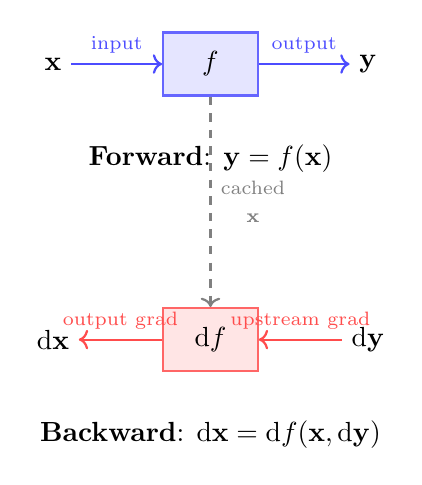
\begin{tikzpicture}[
  node distance=2cm,
  fwdnode/.style={rectangle, draw=blue!60, fill=blue!10, thick, minimum width=1.2cm, minimum height=0.8cm},
  bwdnode/.style={rectangle, draw=red!60, fill=red!10, thick, minimum width=1.2cm, minimum height=0.8cm},
  tensor/.style={},
  fwdarrow/.style={->, thick, blue!70},
  bwdarrow/.style={->, thick, red!70},
  cachearrow/.style={->, thick, dashed, gray}
]

% Forward pass
\node[tensor] (x_fwd) {$\mathbf{x}$};
\node[fwdnode, right of=x_fwd] (f_node) {$f$};
\node[tensor, right of=f_node] (y_fwd) {$\mathbf{y}$};

\draw[fwdarrow] (x_fwd) -- (f_node) node[midway, above] {\scriptsize input};
\draw[fwdarrow] (f_node) -- (y_fwd) node[midway, above] {\scriptsize output};

\node[below of=f_node, node distance=1.2cm] (fwd_label) {\textbf{Forward}: $\mathbf{y} = f(\mathbf{x})$};

% Backward pass
\node[tensor, below of=x_fwd, node distance=3.5cm] (dx_bwd) {$\mathrm{d}\mathbf{x}$};
\node[bwdnode, right of=dx_bwd] (df_node) {$\mathrm{d}f$};
\node[tensor, right of=df_node] (dy_bwd) {$\mathrm{d}\mathbf{y}$};

\draw[bwdarrow] (dy_bwd) -- (df_node) node[midway, above] {\scriptsize upstream grad};
\draw[bwdarrow] (df_node) -- (dx_bwd) node[midway, above] {\scriptsize output grad};

% Cache connection
\draw[cachearrow] (f_node) -- (df_node) node[midway, right, align=center] {\scriptsize cached\\[-2pt]\scriptsize $\mathbf{x}$};

\node[below of=df_node, node distance=1.2cm] (bwd_label) {\textbf{Backward}: $\mathrm{d}\mathbf{x} = \mathrm{d}f(\mathbf{x}, \mathrm{d}\mathbf{y})$};

\end{tikzpicture}
\end{center}

Conceptually, each backward node in the graph implements the local mapping
\[
(\mathbf{x}, \mathrm{d}\mathbf{y}) \mapsto \mathrm{d}\mathbf{x},
\]
where:
\begin{itemize}
\item \textbf{Input 1 (cached)}: The forward input $\mathbf{x}$ is cached during the forward pass
\item \textbf{Input 2 (upstream)}: The upstream gradient $\mathrm{d}\mathbf{y}$ flows from the next layer
\item \textbf{Output}: The resulting local gradient $\mathrm{d}\mathbf{x}$ flows to the previous layer
\end{itemize}

Softmax, dropout, layer normalization, and many other operators in a Transformer layer are special cases of this pattern. Their concrete backward rules are described in terms of such operators $\mathrm{d}f$.

\subsection{Nodes with Multiple Inputs}

Many nodes in a Transformer layer have several inputs. For example, a matrix multiplication node uses both an activation tensor and a weight matrix, and a layer-normalization node uses inputs as well as learned scale and shift parameters. Abstractly, we write
\[
\mathbf{y} = f(\mathbf{x}_1, \mathbf{x}_2, \ldots, \mathbf{x}_k),
\]
where each $\mathbf{x}_i$ may be a tensor of its own.

Given the upstream gradient $\mathrm{d}\mathbf{y} = \partial\mathcal{L}/\partial\mathbf{y}$, the chain rule yields gradients with respect to all inputs,
\[
\mathrm{d}\mathbf{x}_i = \mathbf{J}_{f,\mathbf{x}_i}(\mathbf{x}_1, \ldots, \mathbf{x}_k)^T \mathrm{d}\mathbf{y}, \quad i = 1, \ldots, k,
\]
where $\mathbf{J}_{f,\mathbf{x}_i}$ is the Jacobian of $f$ with respect to the $i$-th input.

We encode this in an abstract backward operator
\[
\mathrm{d}_{\mathbf{x}_i}f(\mathbf{x}_1, \ldots, \mathbf{x}_k, \mathrm{d}\mathbf{y}) := \mathbf{J}_{f,\mathbf{x}_i}(\mathbf{x}_1, \ldots, \mathbf{x}_k)^T \mathrm{d}\mathbf{y},
\]
so that, for each input,
\[
\mathrm{d}\mathbf{x}_i = \mathrm{d}_{\mathbf{x}_i}f(\mathbf{x}_1, \ldots, \mathbf{x}_k, \mathrm{d}\mathbf{y}).
\]

Collecting all input gradients together, we can also view the backward node as a single vector-valued operator
\[
\boxed{(\mathrm{d}\mathbf{x}_1, \ldots, \mathrm{d}\mathbf{x}_k) = \mathrm{d}f(\mathbf{x}_1, \ldots, \mathbf{x}_k, \mathrm{d}\mathbf{y})},
\]
whose components are exactly the individual $\mathrm{d}_{\mathbf{x}_i}f(\cdot, \ldots, \cdot, \mathrm{d}\mathbf{y})$.

\textbf{Example: Matrix Multiplication}

\begin{center}
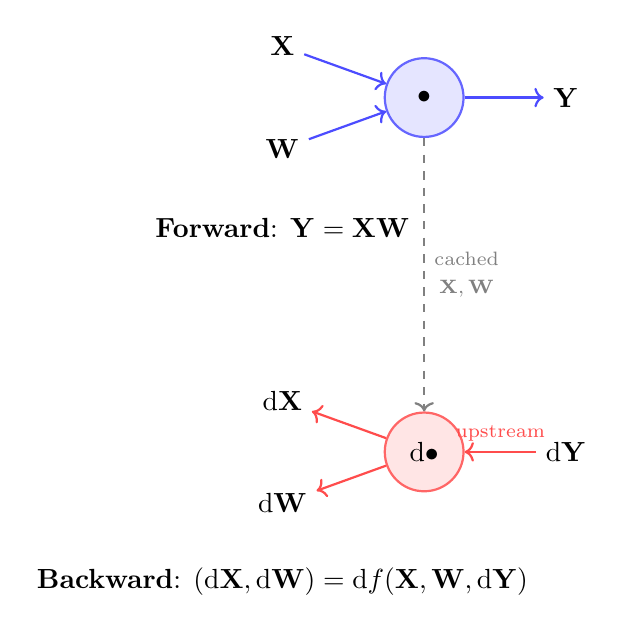
\begin{tikzpicture}[
  node distance=1.8cm,
  fwdnode/.style={circle, draw=blue!60, fill=blue!10, thick, minimum size=1cm},
  bwdnode/.style={circle, draw=red!60, fill=red!10, thick, minimum size=1cm},
  tensor/.style={},
  fwdarrow/.style={->, thick, blue!70},
  bwdarrow/.style={->, thick, red!70},
  cachearrow/.style={->, thick, dashed, gray}
]

% Forward pass
\node[tensor] (x_fwd) {$\mathbf{X}$};
\node[tensor, below of=x_fwd, node distance=1.3cm] (W_fwd) {$\mathbf{W}$};
\node[fwdnode, right of=x_fwd, yshift=-0.65cm] (f_node) {$\bullet$};
\node[tensor, right of=f_node] (y_fwd) {$\mathbf{Y}$};

\draw[fwdarrow] (x_fwd) -- (f_node);
\draw[fwdarrow] (W_fwd) -- (f_node);
\draw[fwdarrow] (f_node) -- (y_fwd);

\node[below of=W_fwd, node distance=1.0cm] (fwd_label) {\textbf{Forward}: $\mathbf{Y} = \mathbf{X}\mathbf{W}$};

% Backward pass
\node[tensor, below of=x_fwd, node distance=4.5cm] (dx_bwd) {$\mathrm{d}\mathbf{X}$};
\node[tensor, below of=W_fwd, node distance=4.5cm] (dW_bwd) {$\mathrm{d}\mathbf{W}$};
\node[bwdnode, right of=dx_bwd, yshift=-0.65cm] (df_node) {$\mathrm{d}\bullet$};
\node[tensor, right of=df_node] (dy_bwd) {$\mathrm{d}\mathbf{Y}$};

\draw[bwdarrow] (dy_bwd) -- (df_node) node[midway, above] {\scriptsize upstream};
\draw[bwdarrow] (df_node) -- (dx_bwd);
\draw[bwdarrow] (df_node) -- (dW_bwd);

% Cache connections
\draw[cachearrow] (f_node) -- (df_node) node[midway, right, align=center] {\scriptsize cached\\[-2pt]\scriptsize $\mathbf{X}, \mathbf{W}$};

\node[below of=dW_bwd, node distance=1.0cm] (bwd_label) {\textbf{Backward}: $(\mathrm{d}\mathbf{X}, \mathrm{d}\mathbf{W}) = \mathrm{d}f(\mathbf{X}, \mathbf{W}, \mathrm{d}\mathbf{Y})$};

\end{tikzpicture}
\end{center}

\vspace{0.3cm}

\noindent
\textbf{Concrete formulas:}
\begin{align*}
\mathrm{d}\mathbf{X} &= \mathrm{d}\mathbf{Y} \mathbf{W}^T \\
\mathrm{d}\mathbf{W} &= \mathbf{X}^T \mathrm{d}\mathbf{Y}
\end{align*}

In the diagrams, this is represented as a single backward node (for example, a node labeled \texttt{dMatmul} or \texttt{dLN}) with multiple incoming edges carrying the necessary forward inputs and the upstream gradient, and multiple outgoing edges carrying $\mathrm{d}\mathbf{x}_1, \ldots, \mathrm{d}\mathbf{x}_k$.

\subsection{Computation Graph and Backpropagation}

A full Transformer layer can be viewed as a composition of simpler operations:
\[
\mathbf{X}_0 \xrightarrow{f_1} \mathbf{X}_1 \xrightarrow{f_2} \mathbf{X}_2 \xrightarrow{\cdots} \mathbf{X}_L,
\]
where $\mathbf{X}_0$ is the input to the layer and $\mathbf{X}_L$ is the final output before the loss. Each $f_\ell$ is a local operator such as a matrix multiplication, a nonlinearity, a dropout, or a normalization.

Backpropagation proceeds in reverse order. Starting from $\mathrm{d}\mathbf{X}_L = \partial\mathcal{L}/\partial\mathbf{X}_L$, we apply the corresponding backward operator for each node:
\[
\mathrm{d}\mathbf{X}_\ell = \mathrm{d}f_\ell(\mathbf{X}_\ell, \mathrm{d}\mathbf{X}_{\ell+1}), \quad \ell = L-1, L-2, \ldots, 0.
\]

\textbf{Graphical representation of a computation chain:}

\begin{center}
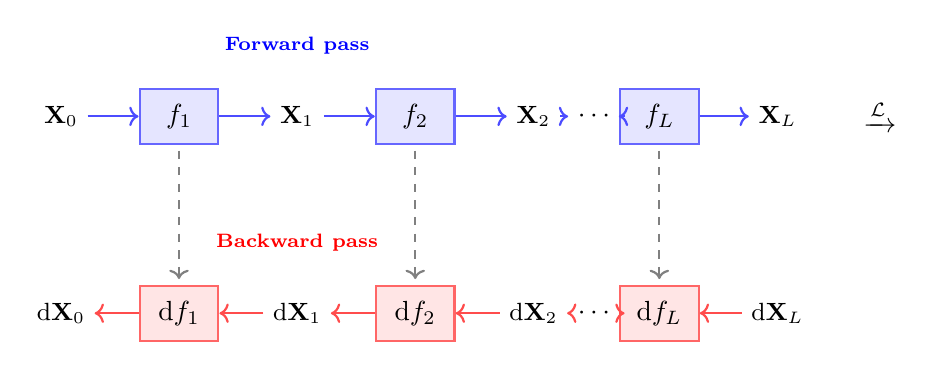
\begin{tikzpicture}[
  node distance=1.5cm,
  fwdnode/.style={rectangle, draw=blue!60, fill=blue!10, thick, minimum width=1cm, minimum height=0.7cm},
  bwdnode/.style={rectangle, draw=red!60, fill=red!10, thick, minimum width=1cm, minimum height=0.7cm},
  tensor/.style={font=\small},
  fwdarrow/.style={->, thick, blue!70},
  bwdarrow/.style={->, thick, red!70},
  cachearrow/.style={->, thick, dashed, gray, shorten >=2pt, shorten <=2pt}
]

% Forward pass
\node[tensor] (x0) {$\mathbf{X}_0$};
\node[fwdnode, right of=x0] (f1) {$f_1$};
\node[tensor, right of=f1] (x1) {$\mathbf{X}_1$};
\node[fwdnode, right of=x1] (f2) {$f_2$};
\node[tensor, right of=f2] (x2) {$\mathbf{X}_2$};
\node[right of=x2, node distance=0.8cm] (dots) {$\cdots$};
\node[fwdnode, right of=dots, node distance=0.8cm] (fL) {$f_L$};
\node[tensor, right of=fL] (xL) {$\mathbf{X}_L$};
\node[right of=xL, node distance=1.3cm] (loss) {$\xrightarrow{\mathcal{L}}$};

\draw[fwdarrow] (x0) -- (f1);
\draw[fwdarrow] (f1) -- (x1);
\draw[fwdarrow] (x1) -- (f2);
\draw[fwdarrow] (f2) -- (x2);
\draw[fwdarrow] (x2) -- (dots);
\draw[fwdarrow] (dots) -- (fL);
\draw[fwdarrow] (fL) -- (xL);

\node[above of=x1, node distance=0.9cm, blue] {\scriptsize\textbf{Forward pass}};

% Backward pass
\node[tensor, below of=x0, node distance=2.5cm] (dx0) {$\mathrm{d}\mathbf{X}_0$};
\node[bwdnode, right of=dx0] (df1) {$\mathrm{d}f_1$};
\node[tensor, right of=df1] (dx1) {$\mathrm{d}\mathbf{X}_1$};
\node[bwdnode, right of=dx1] (df2) {$\mathrm{d}f_2$};
\node[tensor, right of=df2] (dx2) {$\mathrm{d}\mathbf{X}_2$};
\node[right of=dx2, node distance=0.8cm] (bdots) {$\cdots$};
\node[bwdnode, right of=bdots, node distance=0.8cm] (dfL) {$\mathrm{d}f_L$};
\node[tensor, right of=dfL] (dxL) {$\mathrm{d}\mathbf{X}_L$};

\draw[bwdarrow] (dx1) -- (df1);
\draw[bwdarrow] (df1) -- (dx0);
\draw[bwdarrow] (dx2) -- (df2);
\draw[bwdarrow] (df2) -- (dx1);
\draw[bwdarrow] (bdots) -- (dx2);
\draw[bwdarrow] (dxL) -- (dfL);
\draw[bwdarrow] (dfL) -- (bdots);

\node[above of=dx1, node distance=0.9cm, red] {\scriptsize\textbf{Backward pass}};

% Cache arrows
\draw[cachearrow] (f1) -- (df1);
\draw[cachearrow] (f2) -- (df2);
\draw[cachearrow] (fL) -- (dfL);

\end{tikzpicture}
\end{center}

\vspace{0.3cm}

\noindent
Key observations:
\begin{itemize}
\item \textbf{Forward}: Data flows left to right through function nodes $f_\ell$
\item \textbf{Backward}: Gradients flow right to left through backward nodes $\mathrm{d}f_\ell$
\item \textbf{Cache}: Each backward node $\mathrm{d}f_\ell$ needs access to the cached forward state $\mathbf{X}_\ell$
\item \textbf{Chain rule}: $\mathrm{d}\mathbf{X}_\ell = \mathrm{d}f_\ell(\mathbf{X}_\ell, \mathrm{d}\mathbf{X}_{\ell+1})$ for $\ell = L-1, \ldots, 0$
\end{itemize}

If $f_\ell$ depends on additional inputs (e.g. parameters), then its backward operator also produces gradients with respect to those inputs, as discussed below.

In the diagrams, we emphasize this process by drawing:
\begin{itemize}
\item \textbf{forward edges} for $\mathbf{X}_\ell$ flowing into the forward nodes $f_\ell$,
\item \textbf{backward edges} for $\mathrm{d}\mathbf{X}_\ell$ flowing out of the corresponding backward nodes $\mathrm{d}f_\ell$.
\end{itemize}

The detailed formulas that define each local operator $\mathrm{d}f_\ell$ are hidden inside the node and explained in the operator dictionary of Section 4.

\subsection{Parameter Gradients and Updates}

Parameters such as weight matrices and bias vectors enter the graph as additional inputs to some node. For example, consider a matrix multiplication
\[
\mathbf{Y} = \mathbf{X}\mathbf{W},
\]
where $\mathbf{X}$ is an activation tensor and $\mathbf{W}$ is a weight matrix. We view this as a function of two inputs,
\[
\mathbf{Y} = f(\mathbf{X}, \mathbf{W}).
\]

The corresponding backward operator produces both activation and parameter gradients:
\[
\boxed{(\mathrm{d}\mathbf{X}, \mathrm{d}\mathbf{W}) = \mathrm{d}f(\mathbf{X}, \mathbf{W}, \mathrm{d}\mathbf{Y})}.
\]

\textbf{Parameter gradient flow:}

\begin{center}
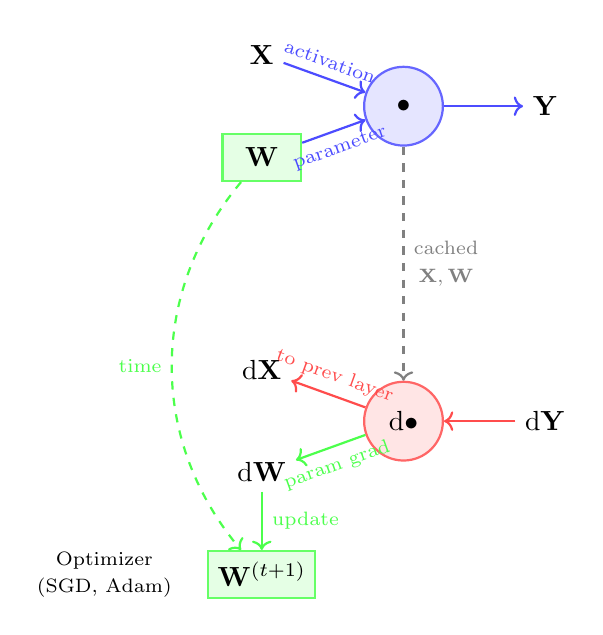
\begin{tikzpicture}[
  node distance=1.8cm,
  fwdnode/.style={circle, draw=blue!60, fill=blue!10, thick, minimum size=1cm},
  bwdnode/.style={circle, draw=red!60, fill=red!10, thick, minimum size=1cm},
  paramnode/.style={rectangle, draw=green!60, fill=green!10, thick, minimum width=1cm, minimum height=0.6cm},
  tensor/.style={},
  fwdarrow/.style={->, thick, blue!70},
  bwdarrow/.style={->, thick, red!70},
  paramarrow/.style={->, thick, green!70},
  cachearrow/.style={->, thick, dashed, gray}
]

% Forward pass
\node[tensor] (x_fwd) {$\mathbf{X}$};
\node[paramnode, below of=x_fwd, node distance=1.3cm] (W_fwd) {$\mathbf{W}$};
\node[fwdnode, right of=x_fwd, yshift=-0.65cm] (f_node) {$\bullet$};
\node[tensor, right of=f_node] (y_fwd) {$\mathbf{Y}$};

\draw[fwdarrow] (x_fwd) -- (f_node) node[midway, above, sloped] {\scriptsize activation};
\draw[fwdarrow] (W_fwd) -- (f_node) node[midway, below, sloped] {\scriptsize parameter};
\draw[fwdarrow] (f_node) -- (y_fwd);

% Backward pass
\node[tensor, below of=x_fwd, node distance=4cm] (dx_bwd) {$\mathrm{d}\mathbf{X}$};
\node[tensor, below of=W_fwd, node distance=4cm] (dW_bwd) {$\mathrm{d}\mathbf{W}$};
\node[bwdnode, right of=dx_bwd, yshift=-0.65cm] (df_node) {$\mathrm{d}\bullet$};
\node[tensor, right of=df_node] (dy_bwd) {$\mathrm{d}\mathbf{Y}$};

\draw[bwdarrow] (dy_bwd) -- (df_node);
\draw[bwdarrow] (df_node) -- (dx_bwd) node[midway, above, sloped] {\scriptsize to prev layer};
\draw[paramarrow] (df_node) -- (dW_bwd) node[midway, below, sloped] {\scriptsize param grad};

% Optimizer
\node[paramnode, below of=dW_bwd, node distance=1.3cm] (W_next) {$\mathbf{W}^{(t+1)}$};
\node[left of=W_next, node distance=2cm, align=center] (opt_label) {\scriptsize Optimizer\\[-2pt]\scriptsize (SGD, Adam)};

\draw[paramarrow] (dW_bwd) -- (W_next) node[midway, right] {\scriptsize update};
\draw[paramarrow, dashed, bend right=40] (W_fwd) to node[midway, left] {\scriptsize time} (W_next);

% Cache connections
\draw[cachearrow] (f_node) -- (df_node) node[midway, right, align=center] {\scriptsize cached\\[-2pt]\scriptsize $\mathbf{X}, \mathbf{W}$};

\end{tikzpicture}
\end{center}

\vspace{0.3cm}

\noindent
An optimizer then uses the parameter gradients to update the parameters. For example, stochastic gradient descent with learning rate $\eta$ performs
\[
\theta^{(t+1)} = \theta^{(t)} - \eta \, \mathrm{d}\theta^{(t)}.
\]

\textbf{Key distinction}:
\begin{itemize}
\item \textbf{Activation gradients} ($\mathrm{d}\mathbf{X}$): Flow to the previous layer in the backward pass
\item \textbf{Parameter gradients} ($\mathrm{d}\mathbf{W}$): Accumulated and used by the optimizer to update weights
\end{itemize}

In this document we do not draw optimizer steps in the diagrams; we only show how $\mathrm{d}\mathbf{W}$ and $\mathrm{d}\mathbf{b}$ are computed by the backward nodes.

\subsection{Connection to the Diagrams}

The detailed MHA, MLP, and output-projection figures in later sections are best read with this abstract picture in mind:
\begin{itemize}
\item Each \textbf{forward node} (e.g. \texttt{SM}, \texttt{S}, \texttt{DO}, \texttt{LN}, \texttt{matmul}) represents a mapping $\mathbf{y} = f(\mathbf{x}_1, \ldots, \mathbf{x}_k)$.
\item Each corresponding \textbf{backward node} (e.g. \texttt{dSM}, \texttt{dS}, \texttt{dDO}, \texttt{dLN}, \texttt{dMatmul}) represents the operator
\[
(\mathrm{d}\mathbf{x}_1, \ldots, \mathrm{d}\mathbf{x}_k) = \mathrm{d}f(\mathbf{x}_1, \ldots, \mathbf{x}_k, \mathrm{d}\mathbf{y}),
\]
implemented using the appropriate Jacobian-transpose formulas for that operator.
\item Edges labeled with tensors such as $\mathbf{X}$, $\mathbf{H}$, $\mathbf{Q}$, $\mathbf{K}$, $\mathbf{V}$, $\mathbf{AS}$, and their gradients $\mathrm{d}\mathbf{X}$, $\mathrm{d}\mathbf{Q}$, $\mathrm{d}\mathbf{W}$, etc., capture only the flow of data, together with compact shape annotations like $[B, S, D]$ or $[B, N_H, S, D_h]$.
\end{itemize}

In the next section we define the graphical notation and operator dictionary used in the figures, and we specialize the abstract backward operator $\mathrm{d}f$ to concrete nodes such as softmax (\texttt{S}/\texttt{dS}), scale/mask (\texttt{SM}/\texttt{dSM}), dropout (\texttt{DO}/\texttt{dDO}), and layer normalization (\texttt{LN}/\texttt{dLN}).

\fi
\clearpage

% ==========================================================
% 4. Graphical Notation and Figure Conventions
% ==========================================================
\ifkorean
  % ==========================================================
% 4. 그래프 표기와 도식 규칙
% ==========================================================
\section{그래프 표기와 도식 규칙}
\label{sec:graph-conventions}

이 문서의 다이어그램은 트랜스포머 레이어 안에서 텐서가 어떻게 흐르는지,
그리고 순전파와 역전파에서 어떤 연산이 수행되는지 \emph{시각적으로} 드러내기 위해 설계되었다.
특히 우리는 다음과 같은 것들을 명확히 보여주고자 한다.
\begin{itemize}
  \item 각 엣지가 어떤 텐서(활성값 또는 기울기)를 나타내는지,
  \item 그 텐서의 차원(예: $[B, S, D]$, $[B, N_H, S, D_h]$ 등)이 무엇인지,
  \item 어떤 노드가 어떤 연산(행렬 곱, softmax, 드롭아웃, 레이어 정규화, 통신, 브로드캐스트 등)에 해당하는지,
  \item 순전파에 대응하는 역전파 연산자가 어떻게 배치되는지.
\end{itemize}

이 장에서는 이러한 그림들을 읽기 위한 기본 규칙을 정리한다.
앞 장에서 소개한 추상적인 순전파/역전파 연산자(Section~\ref{sec:gradients-basics})를,
구체적인 노드와 엣지 표기로 어떻게 구현하는지에 초점을 맞춘다.

\subsection{텐서 차원과 인덱스 표기}

텐서 차원은 항상 \emph{대괄호(brace)}로 묶어서 표기한다.
예를 들어, 본문에서 $\mathbf{X} \in \mathbb{R}^{B \times S \times D}$라고 쓸 때,
그냥 $B \times S \times D$라고 적는 대신, 그림에서는 엣지 옆에
\[
  [B, S, D], \quad [B, N_H, S, D_h], \quad [D, D_{\text{ff}}],
\]
와 같은 라벨을 직접 붙인다.
이렇게 하면 각 엣지가 어떤 차원 순서를 따르는지 바로 확인할 수 있다.

주요 기호는 다음과 같다.
\begin{itemize}
  \item $B$: 배치 크기 (batch size)
  \item $S$: 시퀀스 길이 (sequence length)
  \item $D$: 모델/은닉 차원 (model/hidden dimension)
  \item $N_H$: 어텐션 헤드 수 (number of heads)
  \item $D_h$: 헤드 차원 (head dimension), 보통 $D = N_H \cdot D_h$
  \item $D_{\text{ff}}$: MLP/FFN 내부 피드포워드 차원
\end{itemize}

엣지 라벨은 텐서의 랭크(rank)를 직접 반영한다.
예를 들어,
\begin{itemize}
  \item $[B, S, D]$: 시퀀스 배치 텐서,
  \item $[B, N_H, S, D_h]$: 멀티헤드 어텐션에서 Q/K/V 텐서,
  \item $[B, N_H, S, S]$: 어텐션 스코어 또는 소프트맥스 결과,
  \item $[D, D_{\text{ff}}]$, $[D_{\text{ff}}, D]$: 선형 레이어 가중치.
\end{itemize}

순전파 다이어그램에서는 \emph{왼쪽에서 오른쪽}으로 계산이 진행되며,
엣지 방향은 계산 그래프의 방향을 따른다.
역전파 다이어그램에서는 기울기가 \emph{오른쪽에서 왼쪽}으로 전달되지만,
그림 상에서는 여전히 “기울기 엣지의 방향”을 화살표로 표시하여
순전파 엣지와 구분할 수 있게 한다.

\subsection{순전파·역전파 노드의 추상적 구조}

대부분의 연산자는 추상적으로 다음과 같이 쓸 수 있다.
\[
  \mathbf{y} = f(\mathbf{x}_1, \ldots, \mathbf{x}_k),
\]
여기서 $\mathbf{x}_1, \ldots, \mathbf{x}_k$는 활성값 또는 파라미터(예: 가중치, bias, 정규화 파라미터 등)를 포함한다.

Section~\ref{sec:gradients-basics}에서 소개한 것처럼,
이에 대응하는 역전파 연산자는
\[
  (\mathrm{d}\mathbf{x}_1, \ldots, \mathrm{d}\mathbf{x}_k)
  = \mathrm{d}f(\mathbf{x}_1, \ldots, \mathbf{x}_k, \mathrm{d}\mathbf{y})
\]
의 형태를 가진다.
즉, 순전파 입력들 $\mathbf{x}_i$와 위쪽에서 내려온 기울기 $\mathrm{d}\mathbf{y}$를 받아,
각 입력에 대한 기울기 $\mathrm{d}\mathbf{x}_i$를 계산하는 연산자이다.

이 문서의 다이어그램에서:
\begin{itemize}
  \item 순전파 노드는 $f$를 나타내고,
  \item 역전파 노드는 $\mathrm{d}f$를 나타낸다.
\end{itemize}
노드 안에 쓰인 레이블(예: \texttt{Matmul}, \texttt{SM}, \texttt{LN}, \texttt{dMatmul}, \texttt{dSM}, \texttt{dLN})은
해당 노드가 어떤 구체적인 연산자 $f$ 또는 $\mathrm{d}f$를 구현하는지 가리킨다.

\subsection{노드 유형}

다이어그램에서는 몇 가지 반복적으로 등장하는 노드 유형만 사용한다.
각 노드는 순전파와 역전파에서 서로 짝을 이루며,
연산자 $f$와 그에 대응하는 역전파 연산자 $\mathrm{d}f$로 해석할 수 있다.

\paragraph{행렬 곱 (Matmul).}
행렬 곱 노드는 일반적으로 원(circle) 안에 점 또는 \texttt{Matmul} 레이블로 표시한다.
순전파에서는
\[
  \mathbf{Y} = \mathbf{X} W
\]
와 같은 연산을 나타내며, 역전파 노드(\texttt{dMatmul})는
위쪽 기울기 $\mathrm{d}\mathbf{Y}$와 순전파 입력 $\mathbf{X}, W$를 사용하여
$\mathrm{d}\mathbf{X}$, $\mathrm{d}W$를 계산한다.

\paragraph{원소별 비선형 함수 및 기타 연산.}
GELU, ReLU, sigmoid, softmax, 드롭아웃 등
원소별 또는 축 단위로 작동하는 비선형 함수들은
직사각형 또는 작은 박스 노드로 표현된다.
이들에 대응하는 역전파 노드는 \texttt{dSM}, \texttt{dAct}와 같은 이름으로 나타나며,
마찬가지로 순전파 입력과 위쪽 기울기를 사용해
입력 텐서에 대한 기울기를 계산한다.

\paragraph{합/잔차 연결 (Add / Residual).}
두 텐서를 더하는 연산(예: 잔차 연결)은 플러스 기호가 있는 작은 노드로 표현된다.
순전파에서는
\[
  \mathbf{Y} = \mathbf{X}_1 + \mathbf{X}_2
\]
와 같은 연산에 해당하며,
역전파에서는 $\mathrm{d}\mathbf{Y}$를 두 입력에 그대로 복사하여
$\mathrm{d}\mathbf{X}_1$, $\mathrm{d}\mathbf{X}_2$로 전달한다.

\paragraph{레이어 정규화 (LayerNorm).}
레이어 정규화는 \texttt{LN} 레이블이 있는 노드로 표현된다.
순전파 노드는 입력 텐서를 평균과 분산으로 정규화하고,
학습 가능한 스케일/시프트 파라미터를 적용한다.
역전파 노드(\texttt{dLN})는 입력 텐서와 파라미터에 대한 기울기를 모두 계산한다.

\paragraph{브로드캐스트 (Broadcast).}
브로드캐스트는 $\text{BC}_{\cdot}(\cdot)$과 같은 표기로 표현한다.
예를 들어 $\text{BC}_{B,S}(\mathbf{b})$는
$[D]$ 형태의 bias 벡터를 $[B, S, D]$ 텐서와 더할 수 있도록
배치 차원과 시퀀스 차원 방향으로 개념적으로 확장하는 연산을 나타낸다.
역전파에서는 반대로 합산(summation)을 통해
브로드캐스트 이전 차원으로 기울기를 모은다.

\subsection{통신 노드 (All-Reduce, All-Gather 등)}

텐서 병렬화(TP)와 데이터 병렬화(DP)를 다루기 위해,
우리는 통신 연산을 나타내는 별도의 노드 유형을 사용한다.
대표적인 것은 All-Reduce(\texttt{AR})와 All-Gather(\texttt{AG})이다.

\begin{itemize}
  \item \textbf{All-Reduce (\texttt{AR})}:
        여러 디바이스에 분산된 동일 모양의 텐서를 합산(또는 평균)한 뒤,
        그 결과를 다시 모든 디바이스에 복제하는 연산이다.
        역전파에서는 All-Reduce의 기울기가 다시 All-Reduce로 표현될 수 있다.
  \item \textbf{All-Gather (\texttt{AG})}:
        여러 디바이스에 분할되어 있는 텐서를 한 디바이스 관점에서
        더 큰 축 방향으로 이어 붙이는 연산이다.
        역전파에서는 해당 축 방향으로 기울기를 다시 쪼개어 각 디바이스로 보내는 연산이 된다.
\end{itemize}

다이어그램에서 통신 노드는 일반적인 계산 노드와 동일한 방식으로 그려지지만,
엣지에 붙은 차원 라벨을 통해 \emph{어떤 축이 분할 또는 결합되었는지}를 강조한다.
예를 들어, $[B, S, D/N_T]$에서 $[B, S, D]$로 가는 All-Gather는
“모델 차원 $D$가 $N_T$개 디바이스에 분할되어 있다”는 것을 의미한다.

\subsection{MHA/MLP 상세 도식 읽는 법}

이제까지 정의한 표기법을 바탕으로,
이후 장에서 제시하는 MHA와 MLP의 대형 순전파/역전파 도식을 다음과 같이 읽을 수 있다.
\begin{itemize}
  \item \textbf{엣지}:
        활성값 또는 기울기의 흐름을 나타내며,
        $[B, S, D]$, $[B, N_H, S, D_h]$와 같은 차원 라벨이 붙는다.
  \item \textbf{순전파 노드}:
        \texttt{Matmul}, \texttt{SM}, \texttt{LN}, \texttt{Act} 등은
        각각 국소 함수 $f(\mathbf{x}_1, \ldots, \mathbf{x}_k)$를 계산한다.
  \item \textbf{역전파 노드}:
        \texttt{dMatmul}, \texttt{dSM}, \texttt{dLN} 등은
        대응하는 $\mathrm{d}f(\mathbf{x}_1, \ldots, \mathbf{x}_k, \mathrm{d}\mathbf{y})$를 구현하며,
        모든 입력에 대한 기울기를 출력한다.
  \item \textbf{브로드캐스트 표기}:
        $\text{BC}_{B,S}(\mathbf{b})$와 같이 적힌 라벨은
        낮은 랭크의 텐서를 더 높은 랭크 텐서와 더하기 위해
        개념적으로 확장한 뒤 사용하는 것을 의미한다.
  \item \textbf{통신 노드}:
        \texttt{AR}, \texttt{AG} 노드는 디바이스 간 통신을 나타내며,
        엣지에 붙은 차원 라벨을 통해 어떤 축이 병렬화되어 있는지 확인할 수 있다.
\end{itemize}

이러한 규칙을 사용하면, 독자는 복잡한 MHA/MLP 도식에서도
데이터와 기울기의 흐름, 그리고 통신 패턴을 추적할 수 있다.
필요하다면 각 노드에 대해 하부 수식을 유도할 수 있을 정도로
충분히 정밀하지만, 동시에 전체 구조를 한눈에 파악할 수 있도록
시각적 복잡도는 가능한 한 낮추는 것을 목표로 한다.

\else
  \section{Graphical Notation and Figure Conventions}

The diagrams in this document are designed to show how tensors flow through a Transformer layer and its parallel variants. This section summarizes the graphical notation, including tensor-shape labels, node types, edge styles, and the small operator dictionary for the most common nodes (matmul, softmax, scale/mask, dropout, layer normalization, communication, and broadcast).

Throughout the figures, the goal is to emphasize the flow of tensors along edges. The exact Jacobian matrices for each operation are not drawn; instead, the backward nodes are understood as the abstract operators $\mathrm{d}f$ introduced in Section 3.

\subsection{Tensor Shapes and Index Notation}

We use a consistent braced notation for tensor shapes. Instead of writing $\mathbb{R}^{B \times S \times D}$, we annotate edges in the diagrams with labels such as
\[
[B, S, D], \quad [B, N_H, S, D_h], \quad [D, D_{ff}],
\]
directly next to the arrows. This makes it easier to match each edge to a particular dimension ordering.

The main symbols are:
\begin{itemize}
\item $B$: batch size.
\item $S$: sequence length (number of tokens per sequence).
\item $D$: model (hidden) dimension.
\item $D_{ff}$: intermediate MLP (feed-forward) dimension.
\item $N_H$: number of attention heads.
\item $D_h$: per-head dimension, typically $D_h = D/N_H$.
\end{itemize}

Typical tensor shapes in the diagrams include:
\begin{itemize}
\item $\mathbf{X} \in [B, S, D]$: input or hidden states.
\item $\mathbf{H} \in [B, S, D]$: normalized or intermediate states.
\item $\mathbf{Q}, \mathbf{K}, \mathbf{V} \in [B, N_H, S, D_h]$: projected queries, keys, and values.
\item $\mathbf{AS} \in [B, N_H, S, S]$: attention scores after scaling/masking and softmax.
\item $\mathbf{Y} \in [B, S, D]$: output of a Transformer block or layer.
\end{itemize}

Under tensor parallelism (TP) and data parallelism (DP) we mostly keep the same shape notation on edges. For example, a TP shard that actually stores a slice of width $D/N_T$ may still be labeled $[B, S, D]$ in an end-to-end figure when we want to focus on the logical model dimension rather than the physical shard size. When necessary, shard dimensions such as $[B, S, D/N_T]$ or $[B, N_H/N_T, S, D_h]$ are written explicitly.

Gradients use the same shape conventions. For example:
\[
\mathrm{d}\mathbf{X} \in [B, S, D], \quad \mathrm{d}\mathbf{W}_Q \in [D, D], \quad \mathrm{d}\mathbf{W}_{\text{up}} \in [D, D_{ff}].
\]

\subsection{Nodes, Edges, and Arrow Styles}

The diagrams are drawn as computation graphs. Nodes represent local operations; edges represent tensors flowing between them.

\subsubsection{Forward vs. Backward Arrows}

We distinguish between forward and backward flows:
\begin{itemize}
\item \textbf{Overall flow diagrams} (e.g. the top-level Transformer flow) use:
  \begin{itemize}
  \item solid arrows for forward activations (e.g. $\mathbf{X}$ to $\mathbf{Y}$);
  \item dashed arrows for backward gradients (e.g. $\mathrm{d}\mathbf{Y}$ to $\mathrm{d}\mathbf{X}$).
  \end{itemize}
\item \textbf{Detailed backward diagrams} (e.g. MHA backward, MLP backward) use thicker arrows with different styles (single vs. double) to distinguish:
  \begin{itemize}
  \item gradient flow along the main backward path,
  \item cached forward values reused as secondary inputs to backward nodes.
  \end{itemize}
\end{itemize}

In all cases, the arrow direction follows the direction of computation for forward edges and the direction of gradient propagation for backward edges.

\subsubsection{Node Types}

We use a small set of recurring node types:

\paragraph{Matrix multiplication.} A matrix multiplication node is drawn as a circle containing a dot:
\[
\bullet
\]
In the forward pass this corresponds to an operation such as $\mathbf{Y} = \mathbf{X}\mathbf{W}$. In the backward diagrams the corresponding dNode (e.g. \texttt{dMatmul}) implements the abstract backward operator
\[
(\mathrm{d}\mathbf{X}, \mathrm{d}\mathbf{W}) = \mathrm{d}f(\mathbf{X}, \mathbf{W}, \mathrm{d}\mathbf{Y}),
\]
as described in Section 3.

\paragraph{Addition and residuals.} Elementwise addition is drawn as a circle containing a plus:
\[
+
\]
This is used for bias addition, combining residual connections, and aggregating multiple gradient contributions. Small circles labeled $\sum$ denote explicit summations over batch and/or sequence dimensions (e.g. $\sum_{B,S}$ for bias-gradient accumulation).

\paragraph{Generic rectangular operators.} Many local operations (layer normalization, nonlinearity, dropout, scale/mask, reshape, transpose) are drawn as rectangles with short labels such as \texttt{LN}, \texttt{GL}, \texttt{DO}, \texttt{SM}, \texttt{R}, or \texttt{T}. Their backward counterparts are labeled with a leading ``d'', for example \texttt{dLN}, \texttt{dDO}, \texttt{dSM}. Each such dNode implements the corresponding backward operator $\mathrm{d}f(\cdot, \ldots, \cdot, \mathrm{d}\mathbf{y})$.

\paragraph{Communication nodes.} Distributed communication collectives are drawn as small rectangular nodes with labels such as:
\begin{itemize}
\item \texttt{AR}: All-Reduce.
\item \texttt{AG}: All-Gather.
\end{itemize}
The arrows entering/leaving these nodes indicate which tensors are participating in the collective, and the shape annotations show the logical tensor size before and after the communication.

\subsection{Forward and Backward Nodes: Abstract View}

Most operators in a Transformer layer can be written abstractly as
\[
\mathbf{y} = f(\mathbf{x}_1, \ldots, \mathbf{x}_k),
\]
where $\mathbf{x}_1, \ldots, \mathbf{x}_k$ include both activations and parameters (such as weight matrices or bias vectors). In Section 3 we introduced the abstract backward operators
\[
\mathrm{d}\mathbf{x}_i = \mathrm{d}_{\mathbf{x}_i}f(\mathbf{x}_1, \ldots, \mathbf{x}_k, \mathrm{d}\mathbf{y}), \quad i = 1, \ldots, k.
\]

\textbf{How to read nodes in our diagrams:}

\begin{center}
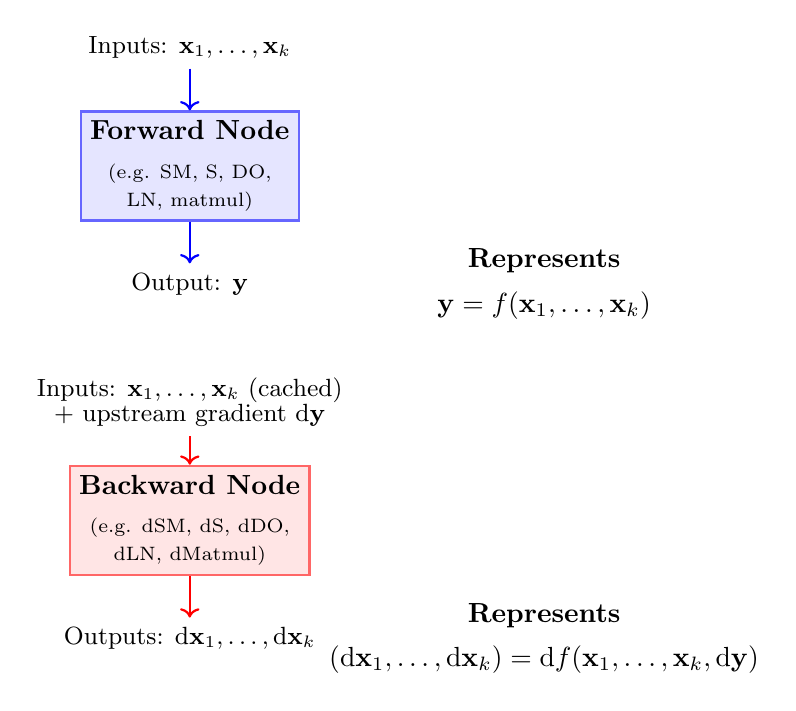
\begin{tikzpicture}[
  node distance=2.5cm,
  fwdnode/.style={rectangle, draw=blue!60, fill=blue!10, thick, minimum width=1.8cm, minimum height=1cm, align=center},
  bwdnode/.style={rectangle, draw=red!60, fill=red!10, thick, minimum width=1.8cm, minimum height=1cm, align=center},
  arrow/.style={->, thick},
  label/.style={font=\small}
]

% Forward node
\node[fwdnode] (fwd) {\textbf{Forward Node}\\[2pt]\scriptsize (e.g. SM, S, DO,\\[-2pt]\scriptsize LN, matmul)};

\node[above of=fwd, node distance=1.5cm, label] (fwd_in) {Inputs: $\mathbf{x}_1, \ldots, \mathbf{x}_k$};
\node[below of=fwd, node distance=1.5cm, label] (fwd_out) {Output: $\mathbf{y}$};

\draw[arrow, blue] (fwd_in) -- (fwd);
\draw[arrow, blue] (fwd) -- (fwd_out);

\node[right of=fwd_out, node distance=4.5cm, align=center] (fwd_eq) {
  \textbf{Represents}\\[4pt]
  $\mathbf{y} = f(\mathbf{x}_1, \ldots, \mathbf{x}_k)$
};

% Backward node
\node[bwdnode, below of=fwd, node distance=4.5cm] (bwd) {\textbf{Backward Node}\\[2pt]\scriptsize (e.g. dSM, dS, dDO,\\[-2pt]\scriptsize dLN, dMatmul)};

\node[above of=bwd, node distance=1.5cm, label, align=center] (bwd_in) {Inputs: $\mathbf{x}_1, \ldots, \mathbf{x}_k$ (cached)\\[-2pt] + upstream gradient $\mathrm{d}\mathbf{y}$};
\node[below of=bwd, node distance=1.5cm, label] (bwd_out) {Outputs: $\mathrm{d}\mathbf{x}_1, \ldots, \mathrm{d}\mathbf{x}_k$};

\draw[arrow, red] (bwd_in) -- (bwd);
\draw[arrow, red] (bwd) -- (bwd_out);

\node[right of=bwd_out, node distance=4.5cm, align=center] (bwd_eq) {
  \textbf{Represents}\\[4pt]
  $(\mathrm{d}\mathbf{x}_1, \ldots, \mathrm{d}\mathbf{x}_k) = \mathrm{d}f(\mathbf{x}_1, \ldots, \mathbf{x}_k, \mathrm{d}\mathbf{y})$
};

\end{tikzpicture}
\end{center}

\vspace{0.3cm}

In the diagrams:
\begin{itemize}
\item A \textbf{forward node} (e.g. \texttt{S}, \texttt{SM}, \texttt{DO}, \texttt{LN}, \texttt{matmul}) represents the mapping $\mathbf{y} = f(\mathbf{x}_1, \ldots, \mathbf{x}_k)$.
\item The corresponding \textbf{backward node} (labeled with a leading ``d'', e.g. \texttt{dS}, \texttt{dSM}, \texttt{dDO}, \texttt{dLN}) represents the mapping
\[
(\mathrm{d}\mathbf{x}_1, \ldots, \mathrm{d}\mathbf{x}_k) = \mathrm{d}f(\mathbf{x}_1, \ldots, \mathbf{x}_k, \mathrm{d}\mathbf{y}),
\]
i.e. it consumes the upstream gradient $\mathrm{d}\mathbf{y}$ and the necessary cached forward inputs, and produces gradients for all inputs.
\end{itemize}

The purpose of this section is not to re-derive all Jacobian formulas, but to provide a dictionary that tells the reader what each node means in the diagrams and how to read its inputs/outputs at the level of tensors and gradients.

\subsection{Operator Dictionary: Forward and Backward}

We now describe the most common node types used in the MHA, MLP, and output-projection diagrams. For each operator we briefly summarize the forward computation and the corresponding backward operator in the abstract notation $\mathrm{d}f(\cdot, \ldots, \cdot, \mathrm{d}\mathbf{y})$.

\subsubsection{Matrix Multiplication (Matmul)}

\textbf{Forward.} A matmul node computes
\[
\mathbf{Y} = \mathbf{X}\mathbf{W},
\]
with shapes such as $\mathbf{X} \in [B, S, D]$, $\mathbf{W} \in [D, D]$, and $\mathbf{Y} \in [B, S, D]$. The same pattern appears in the MLP block with $\mathbf{W}_{\text{up}} \in [D, D_{ff}]$ or $\mathbf{W}_{\text{down}} \in [D_{ff}, D]$.

\textbf{Backward.} The backward node \texttt{dMatmul} implements
\[
(\mathrm{d}\mathbf{X}, \mathrm{d}\mathbf{W}) = \mathrm{d}f(\mathbf{X}, \mathbf{W}, \mathrm{d}\mathbf{Y}),
\]
with the usual formulas
\[
\mathrm{d}\mathbf{X} = \mathrm{d}\mathbf{Y}\mathbf{W}^T, \quad \mathrm{d}\mathbf{W} = \mathbf{X}^T \mathrm{d}\mathbf{Y},
\]
applied with appropriate reshaping for batched tensors. In the diagrams, $\mathbf{X}$ and $\mathbf{W}$ (or their transposes) are supplied to the \texttt{dMatmul} node via double arrows, and outgoing arrows carry $\mathrm{d}\mathbf{X}$ and $\mathrm{d}\mathbf{W}$.

\subsubsection{Broadcast (BC)}

In many diagrams we annotate bias addition by a term such as $\text{BC}_{B,S}(\mathbf{b}_0)$, which denotes a logical broadcast of a 1-D bias vector $\mathbf{b}_0 \in [D]$ or $[D_{ff}]$ across the batch and sequence dimensions to match a tensor of shape $[B, S, D]$ or $[B, S, D_{ff}]$.

\textbf{Forward.} Conceptually,
\[
\mathbf{Y} = \mathbf{X} + \text{BC}_{B,S}(\mathbf{b}_0),
\]
where $\text{BC}_{B,S}(\mathbf{b}_0)$ is a tensor in $[B, S, D]$ obtained by repeating $\mathbf{b}_0$ over the $B$ and $S$ dimensions. In the diagrams we typically draw only the addition node and label the edge near the bias with $\text{BC}_{B,S}(\mathbf{b}_0)$ to indicate that the bias is broadcast in this way.

\textbf{Backward.} The backward contribution to $\mathrm{d}\mathbf{b}_0$ is obtained by summing $\mathrm{d}\mathbf{Y}$ over the broadcast dimensions:
\[
\mathrm{d}\mathbf{b}_0 = \sum_{b=1}^B \sum_{s=1}^S \mathrm{d}\mathbf{Y}_{b,s,:},
\]
which is represented in the diagrams by a small summation node labeled $\sum_{B,S}$. The gradient $\mathrm{d}\mathbf{X}$ simply inherits $\mathrm{d}\mathbf{Y}$, since the addition is symmetric.

\subsubsection{Scale/Mask Node (SM, dSM)}

In the attention mechanism, raw scores $\mathbf{A}$ from $\mathbf{Q}\mathbf{K}^T$ are scaled and masked before softmax. This is represented by a node labeled \texttt{SM} (scale/mask).

\textbf{Forward (SM).} Given attention scores $\mathbf{A} \in [B, N_H, S, S]$, the \texttt{SM} node computes
\[
\mathbf{Z} = \text{SM}(\mathbf{A}) = \alpha \mathbf{A} + \mathbf{M},
\]
where $\alpha = 1/\sqrt{D_h}$ is a scalar and $\mathbf{M}$ encodes the mask (e.g. large negative values at disallowed positions). The shape of $\mathbf{Z}$ matches $\mathbf{A}$. The forward pass caches the scaling factor and the mask pattern.

\textbf{Backward (dSM).} The backward node \texttt{dSM} is the abstract operator
\[
\mathrm{d}\mathbf{A} = \mathrm{d}\text{SM}(\mathbf{A}, \mathrm{d}\mathbf{Z}),
\]
with
\[
\mathrm{d}\text{SM}(\mathbf{A}, \mathrm{d}\mathbf{Z}) = \alpha \, \mathrm{d}\mathbf{Z},
\]
and no gradient is propagated into the fixed mask $\mathbf{M}$. In the diagram, $\mathbf{A}$ and $\mathrm{d}\mathbf{Z}$ enter the \texttt{dSM} node, and $\mathrm{d}\mathbf{A}$ exits as the gradient with respect to the raw attention scores.

\subsubsection{Softmax Node (S, dS)}

The node labeled \texttt{S} performs softmax over the key dimension of the attention scores.

\textbf{Forward (S).} For a fixed batch $b$, head $h$, and query position $s$, let $\mathbf{z} \in \mathbb{R}^S$ be the vector of scores over keys. Softmax produces
\[
\mathbf{p} = \text{softmax}(\mathbf{z}), \quad p_i = \frac{e^{z_i}}{\sum_j e^{z_j}}.
\]
This is applied to every $(b, h, s)$, so the overall shape $[B, N_H, S, S]$ is preserved. The forward pass typically caches $\mathbf{p}$ (or $\mathbf{z}$).

\textbf{Backward (dS).} The backward node \texttt{dS} implements the local mapping
\[
\mathrm{d}\mathbf{z} = \mathrm{d}\text{S}(\mathbf{z}, \mathrm{d}\mathbf{p}),
\]
which, in Jacobian form, is
\[
\mathrm{d}\text{S}(\mathbf{z}, \mathrm{d}\mathbf{p}) = \mathbf{J}_{\text{softmax}}(\mathbf{z})^T \mathrm{d}\mathbf{p}.
\]
In practice this is computed using the standard softmax backward formula. In the diagrams, the \texttt{dS} node has incoming edges carrying $\mathbf{p}$ (or $\mathbf{z}$) and $\mathrm{d}\mathbf{p}$, and an outgoing edge carrying $\mathrm{d}\mathbf{z}$.

\subsubsection{Nonlinearities and Dropout (GL, dGL, DO, dDO)}

Rectangular nodes labeled \texttt{GL}, \texttt{GELU}, or similar denote elementwise nonlinearities; nodes labeled \texttt{DO} denote dropout.

\textbf{Forward (GL / DO).} For a generic scalar nonlinearity $g$,
\[
\mathbf{Y} = g(\mathbf{X})
\]
is applied elementwise. For dropout we write
\[
\mathbf{Y} = \text{DO}(\mathbf{X}; \mathbf{m}) = \mathbf{m} \odot \mathbf{X},
\]
where $\mathbf{m}$ is a binary mask of the same shape as $\mathbf{X}$ and $\odot$ denotes elementwise multiplication. The mask $\mathbf{m}$ is cached in the forward pass.

\textbf{Backward (dGL / dDO).} For a generic nonlinearity, the backward node \texttt{dGL} implements
\[
\mathrm{d}\mathbf{X} = \mathrm{d}\text{GL}(\mathbf{X}, \mathrm{d}\mathbf{Y}) = \mathrm{d}\mathbf{Y} \odot g'(\mathbf{X}),
\]
using the forward input $\mathbf{X}$ from the cache.

For dropout, the backward node \texttt{dDO} implements
\[
\mathrm{d}\mathbf{X} = \mathrm{d}\text{DO}(\mathbf{X}, \mathrm{d}\mathbf{Y}) = \mathbf{m} \odot \mathrm{d}\mathbf{Y}.
\]
In the diagrams, the node labeled \texttt{dDO} consumes the upstream gradient $\mathrm{d}\mathbf{Y}$ and the cached mask $\mathbf{m}$, and produces $\mathrm{d}\mathbf{X}$.

\subsubsection{Layer Normalization (LN, dLN)}

Layer normalization nodes are labeled \texttt{LN} in the forward pass and \texttt{dLN} in the backward pass.

\textbf{Forward (LN).} Given $\mathbf{X} \in [B, S, D]$, layer normalization computes
\[
\mathbf{H} = \text{LN}(\mathbf{X}; \gamma, \beta),
\]
by normalizing each $[D]$-dimensional vector at fixed $B, S$, and applying learned scale and shift parameters $\gamma, \beta \in [D]$. The forward pass caches per-position mean/variance as well as $\gamma$ and $\beta$.

\textbf{Backward (dLN).} The backward node \texttt{dLN} implements
\[
(\mathrm{d}\mathbf{X}, \mathrm{d}\gamma, \mathrm{d}\beta) = \mathrm{d}\text{LN}(\mathbf{X}, \gamma, \beta, \mathrm{d}\mathbf{H}, \text{stats}),
\]
where $\text{stats}$ denotes the cached means and variances. The explicit formulas follow from the standard layer-normalization backward derivation; in the diagrams we treat \texttt{dLN} as a single node that consumes $\mathbf{X}$, $\gamma$, the cached statistics, and $\mathrm{d}\mathbf{H}$, and produces three outgoing gradient edges $\mathrm{d}\mathbf{X}$, $\mathrm{d}\gamma$, and $\mathrm{d}\beta$.

\subsubsection{Communication Nodes (AR, AG)}

In tensor-parallel (TP), data-parallel (DP), and hybrid DP+TP settings, collective communication operations synchronize tensors across devices.

\textbf{All-Reduce (AR).} An All-Reduce node \texttt{AR} takes as input a tensor shard from each participant and outputs the elementwise reduced tensor (typically a sum), optionally divided by the number of participants for averaging. For example, in DP, weight gradients $\mathrm{d}\mathbf{W}$ of shape $[D, D]$ are All-Reduced across all data-parallel ranks before the optimizer step.

\textbf{All-Gather (AG).} An All-Gather node \texttt{AG} concatenates or aggregates tensor shards across a parallel group to reconstruct a full tensor. For example, in TP, partial outputs along a hidden dimension may be gathered to form a full $[B, S, D]$ tensor.

In the diagrams, these communication nodes are treated as pure operators on tensors; their backward behavior (e.g. gradient flow through \texttt{AR} and \texttt{AG}) is implicit in the symmetry of the operations.

\subsection{Reading the Detailed MHA and MLP Figures}

With the conventions above, the large MHA and MLP forward/backward figures can be read as follows:
\begin{itemize}
\item \textbf{Edges} indicate the flow of tensors (activations or gradients), annotated with shapes like $[B, S, D]$ or $[B, N_H, S, D_h]$.
\item \textbf{Forward nodes} (\texttt{S}, \texttt{SM}, \texttt{DO}, \texttt{LN}, \texttt{matmul}, \texttt{reshape}, \texttt{transpose}) compute local functions $f(\mathbf{x}_1, \ldots, \mathbf{x}_k)$.
\item \textbf{Backward nodes} (\texttt{dS}, \texttt{dSM}, \texttt{dDO}, \texttt{dLN}, \texttt{dMatmul}) implement the corresponding backward operators $\mathrm{d}f(\mathbf{x}_1, \ldots, \mathbf{x}_k, \mathrm{d}\mathbf{y})$, producing gradients for all inputs.
\item \textbf{Broadcast labels} such as $\text{BC}_{B,S}(\mathbf{b}_0)$ indicate that a bias vector is conceptually expanded to match a higher-rank tensor before addition.
\item \textbf{Communication nodes} (\texttt{AR}, \texttt{AG}) indicate where collective operations occur in TP, DP, or DP+TP settings, and their shape annotations show the logical dimensions involved.
\end{itemize}

These conventions allow the reader to understand the data and gradient flows at a glance, without being distracted by low-level indexing, while still being precise enough to derive the underlying equations when needed.

\fi
\clearpage

% ==========================================================
% 5. Single-Node Transformer: Forward and Backward
% ==========================================================
\ifkorean
  % ==========================================================
% 5. 단일 노드 트랜스포머: 순전파와 역전파
% ==========================================================
\section{단일 노드 트랜스포머: 순전파와 역전파}
\label{sec:sn}

이 장에서는 병렬화를 전혀 사용하지 않는 \emph{단일 노드(single-node)} 환경에서
하나의 트랜스포머 레이어가 어떻게 동작하는지 정리한다.
순전파와 역전파 모두에 대해 텐서의 모양과 데이터 흐름을 중심으로 설명하며,
각 구성요소를 분리해서 살펴본다.

다루는 주요 구성 요소는 다음과 같다.
\begin{itemize}
  \item \textbf{입력 임베딩 레이어}: 토큰 ID를 연속 벡터 표현으로 변환.
  \item \textbf{멀티헤드 어텐션(MHA)}: 시퀀스 내 위치들 사이의 어텐션 계산.
  \item \textbf{피드포워드 네트워크(MLP/FFN)}: 위치별 비선형 변환.
  \item \textbf{출력 프로젝션과 손실}: 은닉 상태를 로그릿으로投영하고 손실 계산.
\end{itemize}

우리는 배치 크기가 $B$, 시퀀스 길이가 $S$인 토큰 ID 배치
$\mathbf{T} \in [B,S]$가 주어진다고 가정한다.
레이어 내부의 은닉 표현은 보통
\[
  \mathbf{X} \in \mathbb{R}^{B \times S \times D}
\]
와 같이 표현되며, 여기서 $D$는 모델(은닉) 차원이다.
역전파에서는 스칼라 손실 $\mathcal{L}$에 대한 기울기가
이러한 텐서들과 대응되는 가중치 행렬들을 따라 어떻게 흐르는지를 추적한다.

% ------------------------ 5.0 Overall Layer Flow ---------------------

\subsection{전체 트랜스포머 레이어 흐름}

각 구성 요소를 개별적으로 보기 전에,
단일 노드 트랜스포머 레이어 전체에서 순전파와 역전파가 어떻게 흘러가는지
상위 수준에서 먼저 살펴보자.
Figure~\ref{fig:single_node_overall}은
입력 임베딩으로부터 MHA, MLP, 출력 프로젝션을 거쳐 손실에 이르는
순전파 경로와, 다시 손실에서 역전파되어 입력 임베딩까지 전파되는
기울기 흐름을 한 그림에 요약한 것이다.

\begin{figure}[htbp]
  \centering
  \resizebox{\linewidth}{!}{%
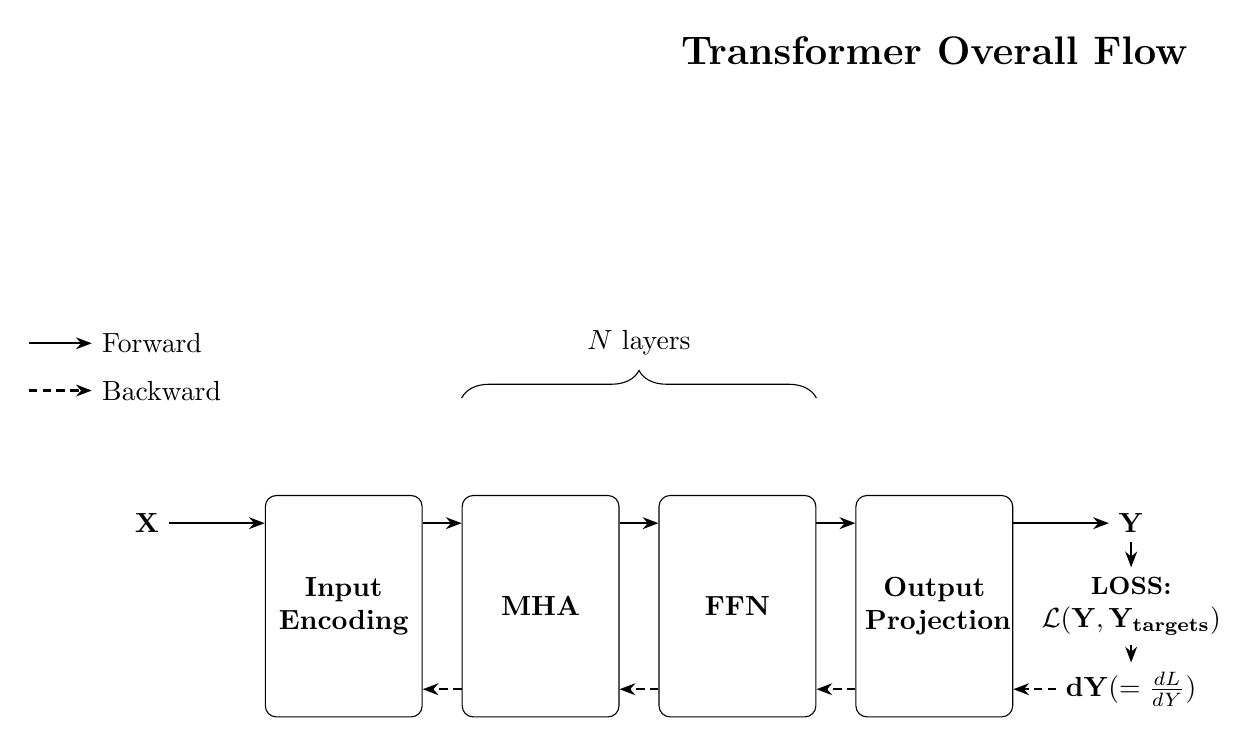
\begin{tikzpicture}[
    node distance=2.5cm,
    >=stealth,
    block/.style={rectangle, draw=black, fill=white, text width=5em, text centered, rounded corners, minimum height=8em, font=\bfseries},
    forward/.style={-{Stealth[length=2mm]}, thick, black},
    backward/.style={-{Stealth[length=2mm]}, thick, black, densely dashed},
    io/.style={text centered, font=\bfseries}
]
    % Title
    \node[font=\Large\bfseries] at (10, 6) {Transformer Overall Flow};

    % Forward path nodes (horizontal)
    \node (input) [io] {$\mathbf{X}$};
    \node (encoding) [block, right of=input, yshift=-3em] {Input\\Encoding};
    \node (mha) [block, right of=encoding] {MHA};
    \node (mlp) [block, right of=mha] {FFN};
    \node (output) [block, right of=mlp] {Output\\Projection};
    \node (pred) [io, right of=output, yshift=3em] {$\mathbf{Y}$};
    \node (loss) [align=center, io, right of=output] {\small LOSS:\\$\mathcal{L}(\mathbf{Y,Y_\text{targets}})$};
    \node (gradient) [io, right of=output, yshift=-3em] {$\mathbf{dY}(=\frac{dL}{dY})$};

    % Forward arrows (upper part of blocks)
    \draw [forward] (input) -- ([yshift=3em]encoding.west);
    \draw [forward] ([yshift=3em]encoding.east) -- ([yshift=3em]mha.west);
    \draw [forward] ([yshift=3em]mha.east) -- ([yshift=3em]mlp.west);
    \draw [forward] ([yshift=3em]mlp.east) -- ([yshift=3em]output.west);
    \draw [forward] ([yshift=3em]output.east) -- (pred);
    \draw [forward] (pred) -- (loss);
    \draw [backward] (loss) -- (gradient);

    % Backward arrows (lower part of blocks)
    \draw [backward] (gradient) -- ([yshift=-3em]output.east);
    \draw [backward] ([yshift=-3em]output.west) -- ([yshift=-3em]mlp.east);
    \draw [backward] ([yshift=-3em]mlp.west) -- ([yshift=-3em]mha.east);
    \draw [backward] ([yshift=-3em]mha.west) -- ([yshift=-3em]encoding.east);

    % Brace for layer repetition
    \draw[decorate, decoration={brace, amplitude=10pt}]
        ([yshift=3.5em]mha.north west) -- ([yshift=3.5em]mlp.north east)
        node[midway, above=12pt, font=\normalsize] {$N$ layers};

    % Labels (Legend)
    \coordinate (legend) at ([xshift=-1.5cm, yshift=6.5em]input);
    \draw[forward] (legend) -- ++(0.8,0) node[right, font=\normalsize] {Forward};
    \draw[backward] ([yshift=-0.6cm]legend) -- ++(0.8,0) node[right, font=\normalsize] {Backward};

\end{tikzpicture}%
}
  \caption{단일 노드 트랜스포머 레이어의 전체 순전파 및 역전파 흐름.
  실선 화살표는 순전파 활성값을, 점선 화살표는 손실 $\mathcal{L}$로부터
  출력 프로젝션, MLP, MHA를 거쳐 입력 임베딩으로 되돌아가는 기울기 흐름을
  나타낸다.}
  \label{fig:single_node_overall}
\end{figure}


% ------------------------ 5.1 Input Embedding ------------------------

\subsection{입력 임베딩 레이어}

입력 임베딩 레이어는 이산적인 토큰 ID를 연속 벡터 표현으로 변환하여,
트랜스포머 스택의 첫 번째 은닉 상태
$\mathbf{X} \in \mathbb{R}^{B \times S \times D}$를 만들어낸다.
다음과 같은 파라미터를 사용한다고 가정한다.
\begin{itemize}
  \item 토큰 임베딩 행렬 $\mathbf{E} \in \mathbb{R}^{V \times D}$:
        $V$는 어휘(vocabulary) 크기.
  \item 위치 임베딩 테이블 $\mathbf{P} \in \mathbb{R}^{S \times D}$:
        학습 가능한 테이블이거나 사인/코사인 기반의 고정 테이블.
\end{itemize}

토큰 ID 배치 $\mathbf{T} \in [B,S]$가 주어졌을 때, 임베딩 레이어는 개념적으로
다음과 같은 연산을 수행한다.
\begin{itemize}
  \item 각 위치 $(b,s)$에 대해 토큰 ID $\mathbf{T}[b,s]$를
        토큰 임베딩 행렬 $\mathbf{E}$의 해당 행으로 매핑하여
        토큰 임베딩 벡터를 얻는다.
  \item 시퀀스 위치 $s$에 대응하는 위치 임베딩 $\mathbf{P}[s,:]$를
        토큰 임베딩에 더한다.
  \item 필요하다면 드롭아웃을 적용하여 초기 은닉 상태
        $\mathbf{X} \in [B,S,D]$를 얻는다.
\end{itemize}

\begin{figure}[htbp]
  \centering
  \documentclass{article}

\usepackage{amsmath, amssymb}
\usepackage{tikz}
\usepackage{graphicx}
\usepackage{caption}
\usepackage[margin=1in, landscape]{geometry}
\usetikzlibrary{shapes, arrows, positioning, fit, calc}

\begin{document}

% ---------- Input Embedding -> (to MHA) ----------
\noindent
\resizebox{\linewidth}{!}{%
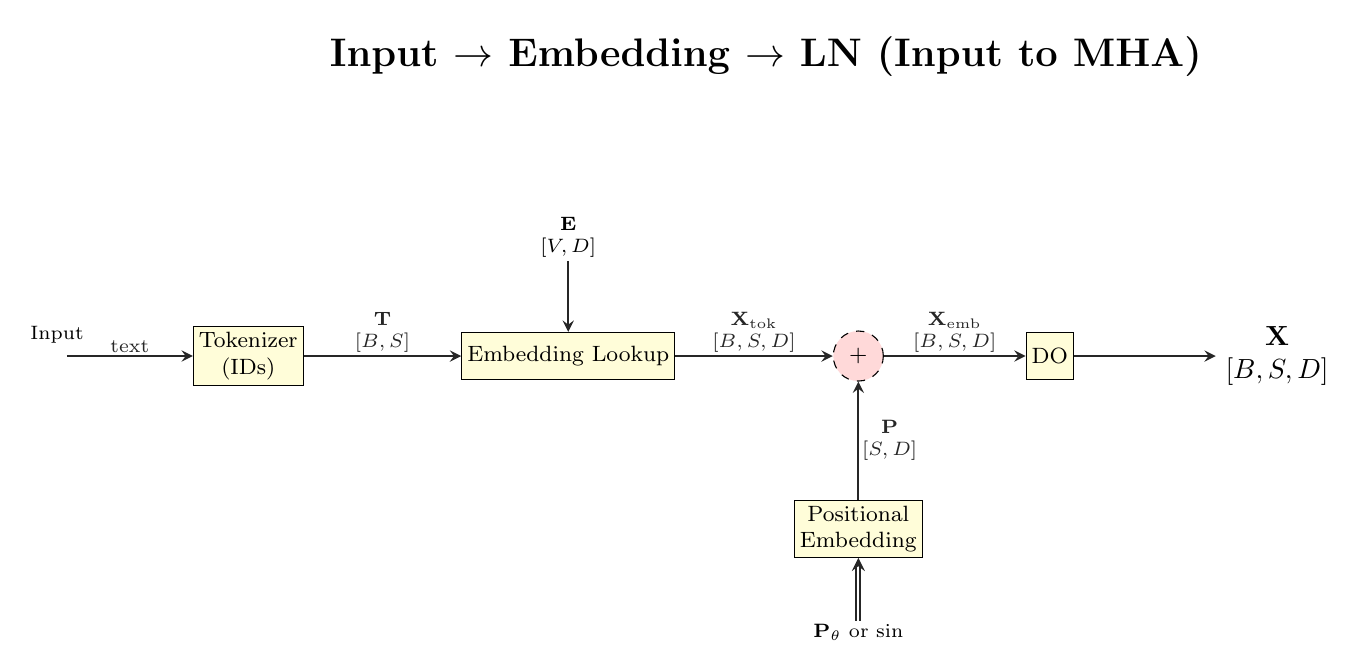
\begin{tikzpicture}[
  >=stealth,
  auxnode/.style={draw, rectangle, fill=yellow!15, minimum height=6mm, inner sep=2pt, font=\footnotesize, align=center},
  mulnode/.style={draw, circle, fill=green!15, minimum size=6mm, font=\footnotesize, align=center},
  addnode/.style={draw, circle, dashed, fill=red!15, minimum size=6mm, font=\footnotesize, align=center},
  flow/.style={->, thick, black!85},
  flow2/.style={->, double, thick, black!85},
  dimlabel/.style={font=\scriptsize, inner sep=1pt, align=center}
]

\node[font=\Large\bfseries] at (9, 3.8) {Input $\rightarrow$ Embedding $\rightarrow$ LN (Input to MHA)};

% nodes
\node (RawText) at (0,0) {};
\node[auxnode, align=center] (Tok)   [right=1.6cm of RawText] {Tokenizer\\(IDs)};
\node[auxnode, align=center] (Lookup)[right=2.0cm of Tok]     {Embedding Lookup};
\node[addnode, minimum size=6mm] (Sum) [right=2.0cm of Lookup] {+};
\node[auxnode, align=center] (PosE)  [below=1.5cm of Sum]  {Positional\\Embedding};
\node[auxnode] (Drop) [right=1.8cm of Sum] {DO};
\node (OUTPUT)   [align=center, right=1.8cm of Drop]   {$\mathbf{X}$\\$[B,S,D]$};

% parameter/const “double” edges
\node[dimlabel] (Eparam) [align=center, above=0.9cm of Lookup] {$\mathbf{E}$\\$[V,D]$};
\node[dimlabel] (Pparam) [align=center, below=0.8cm of PosE]   {$\mathbf{P}_{\theta}$ or sin};

% flows
\draw[flow] (RawText) -- (Tok) node[dimlabel, midway, above]
  {$\text{text}$};
\draw[flow] (Tok) -- (Lookup) node[dimlabel, midway, above]
  {$\mathbf{T}$\\$[B,S]$};

% Embedding matrix E
\draw[flow] (Eparam) -- (Lookup);

% Lookup -> Sum (token embeddings)
\draw[flow] (Lookup) -- (Sum) node[dimlabel, midway, above]
  {$\mathbf{X}_{\text{tok}}$\\$[B,S,D]$};

% Positional embedding path
\draw[flow] (PosE) -- (Sum) node[dimlabel, midway, right]
  {$\mathbf{P}$\\$[S,D]$};

% Optional: show P as parameter (sinusoidal/learned)
\draw[flow2] (Pparam) -- (PosE) ;

\draw[flow] (Sum) -- (Drop) node[dimlabel, midway, above]
  {$\mathbf{X}_{\text{emb}}$\\$[B,S,D]$};
\draw[flow] (Drop) -- (OUTPUT);

% labels for start and destination
\node[dimlabel, above=0.0cm of RawText] {Input};

\end{tikzpicture}%
}

\newpage
\renewcommand{\arraystretch}{1.2}
\small

% -------- Operations (Ops) --------
\begin{center}
\textbf{Operations (Ops)}
\begin{tabular}{llll}
\hline
\textbf{Abbrev} & \textbf{Name} & \textbf{Type / Shape} & \textbf{Notes} \\
\hline
Tokenizer & Tokenizer (IDs) & op & Maps raw text $\to$ integer ids $\mathbf{T}\in\mathbb{Z}^{[B,S]}$. \\
Embedding Lookup & Embedding Lookup & op & Gathers rows from $\mathbf{E}\in\mathbb{R}^{V\times D}$ using ids $\mathbf{T}$. \\
$+$ & Element-wise Add (dashed circle) & op & Adds token and positional embeddings; broadcasting over $B,S$ if needed. \\
DO & Dropout & op & Training-time stochastic dropout on $\mathbf{X}_{\text{emb}}$; identity at inference. \\
\textit{(none)} & Broadcast $\mathrm{BC}_{B,S}(\cdot)$ & op & Expands $[S,D]$ (or $[D]$) to $[B,S,D]$ across batch/sequence. \\
\hline
\end{tabular}
\end{center}

\vspace{0.8em}

% -------- Data Tensors (Values) --------
\begin{center}
\textbf{Data Tensors (Values)}
\begin{tabular}{llll}
\hline
\textbf{Symbol} & \textbf{Name} & \textbf{Shape} & \textbf{Notes} \\
\hline
text & Raw input text & — & Character/byte stream before tokenization. \\
$\mathbf{T}$ & Token ids & $[B,S]$ & Output of Tokenizer; integers in $\{0,\dots,V{-}1\}$. \\
$\mathbf{E}$ & Embedding matrix (params) & $[V,D]$ & Trainable; each vocab entry has a $D$-dim vector. \\
$\mathbf{X}_{\text{tok}}$ & Token embeddings & $[B,S,D]$ & $\mathrm{lookup}(\mathbf{E}, \mathbf{T})$. \\
$\mathbf{P}$ & Positional embedding & $[S,D]$ (or $[B,S,D]$) & Learned $\mathbf{P}_\theta$ \textbf{or} sinusoidal (fixed); broadcast to $[B,S,D]$. \\
$\mathbf{X}_{\text{emb}}$ & Sum of token+pos & $[B,S,D]$ & $\mathbf{X}_{\text{tok}} + \mathrm{BC}_{B,S}(\mathbf{P})$. \\
$\mathbf{X}$ & Input to MHA & $[B,S,D]$ & After dropout (DO); goes to LN/MHA stack. \\
$\mathbf{P}_\theta$ & Learned pos. params & matches $\mathbf{P}$ & Used when positions are trainable; otherwise “sin” denotes fixed sinusoidal. \\
\hline
\multicolumn{4}{l}{\textbf{Shape symbols:}\; $B$=batch size,\; $S$=sequence length,\; $D$=model dim,\; $V$=vocab size.} \\
\multicolumn{4}{l}{\textbf{Notes:}\; In practice, $\mathbf{P}$ may be pre-broadcast to $[B,S,D]$ or added per-token with implicit broadcasting.} \\
\hline
\end{tabular}
\end{center}

\end{document}

  \caption{입력 임베딩 레이어의 순전파.
  토큰 ID는 임베딩 행렬 $\mathbf{E}$를 통해 토큰 임베딩으로 변환되고,
  위치 임베딩 $\mathbf{P}$가 더해진 뒤, (선택적인) 드롭아웃을 거쳐
  초기 은닉 상태 $\mathbf{X} \in [B,S,D]$를 생성한다.}
  \label{fig:single_node_input_embedding}
\end{figure}

역전파에서는 손실 $\mathcal{L}$에 대한 기울기가
$\mathrm{d}\mathbf{X}$로부터 각 임베딩 파라미터로 전파된다.
토큰 임베딩 행렬 $\mathbf{E}$와 위치 임베딩 테이블 $\mathbf{P}$에 대한 기울기는,
각 위치에서 해당 임베딩이 사용된 횟수를 따라 합산(summing)하여 누적된다.
즉, 같은 토큰 ID나 위치가 여러 번 등장하면,
그 위치들로부터의 기울기가 같은 임베딩 파라미터에 더해진다.

% ------------------------ 5.2 Multi-Head Attention -------------------

\subsection{멀티헤드 어텐션 (MHA)}

멀티헤드 어텐션은 모델이 서로 다른 표현 하위공간에서
여러 위치의 정보를 동시에 참조할 수 있게 해주는 메커니즘이다.
구성 요소 관점에서 보면 다음과 같이 나눌 수 있다.
\begin{itemize}
  \item \textbf{선형 프로젝션}: 입력을 쿼리(Q), 키(K), 값(V)로 투영.
  \item \textbf{스케일된 내적 어텐션}: 쿼리–키 내적을 통해 어텐션 스코어를 계산하고,
        소프트맥스로 정규화한 뒤, 값 벡터의 가중합을 계산.
  \item \textbf{멀티헤드 분할}: $N_H$개의 헤드를 병렬로 처리하며,
        각 헤드의 차원은 $D_h$이고 전체 모델 차원은 $D = N_H D_h$.
  \item \textbf{출력 프로젝션}: 각 헤드 출력을 다시 결합(concatenate)한 뒤,
        모델 차원 $D$로 되돌리는 선형 레이어.
\end{itemize}

\subsubsection{순전파}

MHA 블록의 입력은 이전 블록(입력 임베딩 또는 앞선 레이어)의 출력인
\[
  \mathbf{X} \in \mathbb{R}^{B \times S \times D}
\]
이다.
우리는 다음과 같은 순서를 따른다.

\paragraph{(1) 입력 레이어 정규화.}
먼저 은닉 차원 방향으로 레이어 정규화(layer normalization)를 적용한다.
\[
  \mathbf{X}_{\text{norm}} = \mathrm{LN}(\mathbf{X})
  \in \mathbb{R}^{B \times S \times D}.
\]
레이어 정규화는 학습 가능한 스케일/시프트 파라미터
$\boldsymbol{\gamma}, \boldsymbol{\beta} \in \mathbb{R}^{D}$를 가지지만,
도식에서는 주로 정규화된 활성값 $\mathbf{X}_{\text{norm}}$에 초점을 맞춘다.

\paragraph{(2) Q/K/V 선형 프로젝션.}
정규화된 입력에 세 개의 선형 레이어를 적용하여
쿼리, 키, 값 텐서를 생성한다.
\[
  \mathbf{Q} = \mathbf{X}_{\text{norm}} W_Q, \quad
  \mathbf{K} = \mathbf{X}_{\text{norm}} W_K, \quad
  \mathbf{V} = \mathbf{X}_{\text{norm}} W_V.
\]
각 가중치 행렬은 보통
$W_Q, W_K, W_V \in \mathbb{R}^{D \times D}$ 또는
헤드 차원을 고려한 적절한 모양을 가진다.
이후 표현을 위해
$\mathbf{Q}, \mathbf{K}, \mathbf{V}$를
\[
  \mathbf{Q}, \mathbf{K}, \mathbf{V}
  \in \mathbb{R}^{B \times N_H \times S \times D_h}
\]
와 같이 헤드 차원을 명시적으로 드러내는 형태로 재배열(shaping)한다.

\paragraph{(3) 스케일된 내적 어텐션.}
각 헤드 $h$에 대해, 쿼리와 키의 스케일된 내적을 통해 어텐션 스코어를 계산한다.
\[
  \mathbf{A}[b,h,s,t]
  = \frac{1}{\sqrt{D_h}}\,
    \mathbf{Q}[b,h,s,:] \cdot \mathbf{K}[b,h,t,:],
\]
여기서 $s$는 쿼리 위치, $t$는 키 위치이다.
소프트맥스를 시퀀스 축 $t$에 대해 적용하여
어텐션 가중치 $\mathbf{W}_{\text{att}}$를 얻고,
이를 값 텐서 $\mathbf{V}$에 곱해 각 위치의 출력 벡터를 계산한다.
이 연산들의 결과는
\[
  \mathbf{A}_{\text{heads}}
  \in \mathbb{R}^{B \times N_H \times S \times D_h}
\]
와 같은 형태를 가진다.

\paragraph{(4) 헤드 결합 및 출력 프로젝션.}
헤드 차원 방향으로 모든 헤드를 이어 붙여(concatenate) 하나의 텐서로 만들고,
이를 다시 모델 차원 $D$로 투영하는 선형 레이어를 적용한다.
\[
  \mathbf{A}_{\text{out}} = \mathrm{MHA}(\mathbf{X}) \in \mathbb{R}^{B \times S \times D}.
\]
이 텐서는 이후 MLP 블록으로 전달되는 어텐션 출력이다.
도식에서는 각 엣지에 위에서 설명한 텐서 모양이 함께 표시된다
(Figure~\ref{fig:single_node_mha_forward} 참고).

\begin{landscape}
\begin{figure}[htbp]
  % \centering
  \resizebox{\linewidth}{!}{%
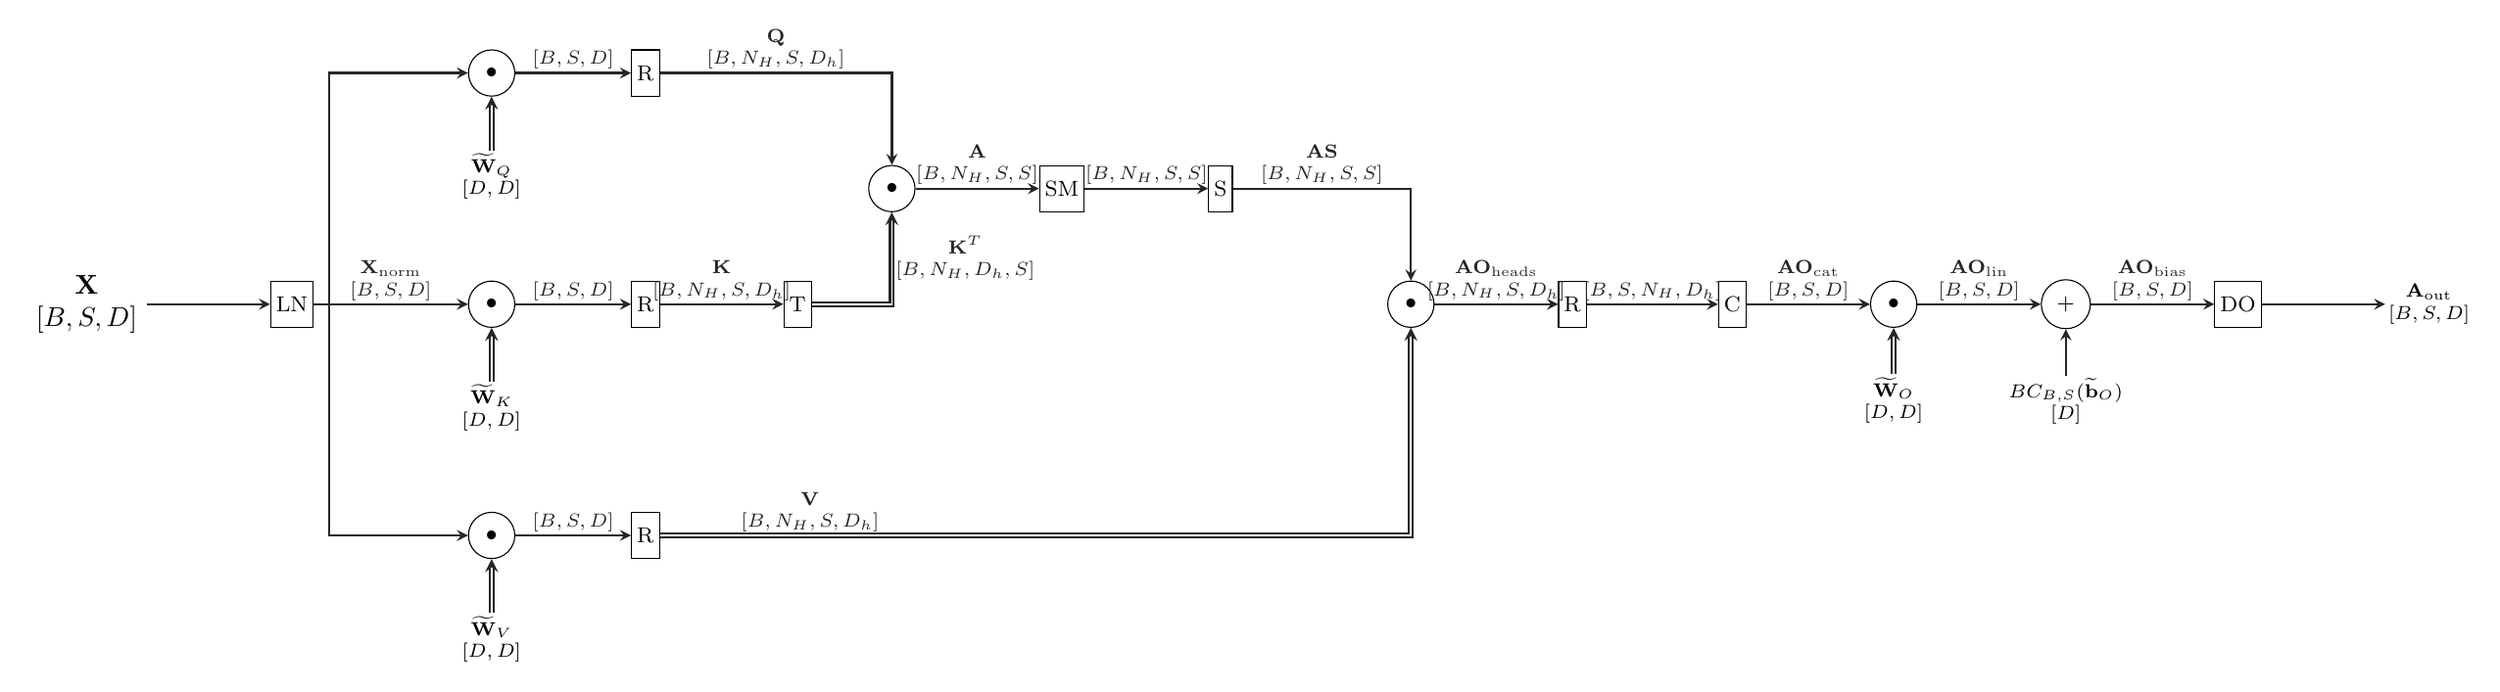
\begin{tikzpicture}[
  every node/.style={transform shape},
  >=stealth,
  auxnode/.style={draw, rectangle, fill=white, minimum height=6mm, inner sep=2pt, font=\footnotesize, align=center},
  mulnode/.style={draw, circle, fill=white, minimum size=6mm, font=\footnotesize, align=center},
  addnode/.style={draw, circle, fill=white, minimum size=6mm, font=\footnotesize, align=center},
  flow/.style={->, thick, black!85},
  flow2/.style={->, double, thick, black!85},
  dimlabel/.style={font=\scriptsize, inner sep=1pt, align=center}
]
% \node[font=\Large\bfseries] at (8, 4.5) {Multi-Head Attention Forward Pass};

\node (Input) at (0.5, 0) [align=center] {$\mathbf{X}$\\$[B,S,D]$};
\node[auxnode] (LN) [right=1.6cm of Input] {LN};

\node[mulnode] (Proj_Q) [right=2.0cm of LN, yshift=3.0cm] {$\bullet$};
\node[auxnode] (R_Q) [right=1.5cm of Proj_Q] {R};

\node[mulnode] (Proj_K) [right=2.0cm of LN, yshift=0cm] {$\bullet$};
\node[auxnode] (R_K) [right=1.5cm of Proj_K] {R};

\node[mulnode] (Proj_V) [right=2.0cm of LN, yshift=-3.0cm] {$\bullet$};
\node[auxnode] (R_V) [right=1.5cm of Proj_V] {R};

\node[dimlabel] (WQ) [align=center, below=0.7cm of Proj_Q] {$\widetilde{\mathbf{W}}_{Q}$\\$[D,D]$};
\node[dimlabel] (WK) [align=center, below=0.7cm of Proj_K] {$\widetilde{\mathbf{W}}_{K}$\\$[D,D]$};
\node[dimlabel] (WV) [align=center, below=0.7cm of Proj_V] {$\widetilde{\mathbf{W}}_{V}$\\$[D,D]$};

\node[auxnode] (T_K) [right=1.6cm of R_K] {T};
\node[mulnode] (QK) [right=2.7cm of R_Q, yshift=-1.5cm] {$\bullet$};
\node[auxnode] (SM) [right=1.6cm of QK] {SM};
\node[auxnode] (Soft) [right=1.6cm of SM] {S};
\node[mulnode] (PV) [right=2.0cm of Soft, yshift=-1.5cm] {$\bullet$};

\node[auxnode] (R_Merge) [right=1.6cm of PV] {R};
\node[auxnode] (Cat) [right=1.7cm of R_Merge] {C};

\node[mulnode] (OProj) [right=1.6cm of Cat] {$\bullet$};
\node[dimlabel] (WO_FWD) [align=center, below=0.6cm of OProj] {$\widetilde{\mathbf{W}}_{O}$\\$[D,D]$};
\node[addnode] (AddB) [right=1.6cm of OProj] {+};
\node[dimlabel] (BO) [align=center, below=0.6cm of AddB] {$BC_{B,S}(\widetilde{\mathbf{b}}_{O})$\\$[D]$};
\node[auxnode] (Drop) [right=1.6cm of AddB] {DO};
\node[dimlabel] (Aout) [align=center, right=1.6cm of Drop] {$\mathbf{A}_{\text{out}}$\\$[B,S,D]$};

\draw[flow] (Input) -- (LN);

\draw[flow] (LN.east) -- ++(0.2,0) |- (Proj_Q.west);
\draw[flow] (LN) -- (Proj_K.west) node[dimlabel, midway, above]{$\mathbf{X}_{\text{norm}}$\\$[B,S,D]$};
\draw[flow] (LN.east) -- ++(0.2,0) |- (Proj_V.west);

\draw[flow2] (WQ) -- (Proj_Q);
\draw[flow2] (WK) -- (Proj_K);
\draw[flow2] (WV) -- (Proj_V);

\draw[flow] (Proj_Q) -- (R_Q) node[dimlabel, midway, above]{$[B,S,D]$};
\draw[flow] (Proj_K) -- (R_K) node[dimlabel, midway, above]{$[B,S,D]$};
\draw[flow] (Proj_V) -- (R_V) node[dimlabel, midway, above]{$[B,S,D]$};

\draw[flow] (R_Q) -| (QK) node[dimlabel, near start, above]{$\mathbf{Q}$\\$[B,N_H,S,D_h]$};
\draw[flow] (R_K) -- (T_K) node[dimlabel, midway, above]{$\mathbf{K}$\\$[B,N_H,S,D_h]$};
\draw[flow2] (T_K) -| (QK) node[dimlabel, near end, right]{$\mathbf{K}^{T}$\\$[B,N_H,D_h,S]$};

\draw[flow] (QK) -- (SM) node[dimlabel, midway, above]{$\mathbf{A}$\\$[B,N_H,S,S]$};
\draw[flow] (SM) -- (Soft) node[dimlabel, midway, above]{$[B,N_H,S,S]$};
\draw[flow] (Soft) -| (PV) node[dimlabel, near start, above]{$\mathbf{AS}$\\$[B,N_H,S,S]$};
\draw[flow2] (R_V) -| (PV) node[dimlabel, pos=0.1, above]{$\mathbf{V}$\\$[B,N_H,S,D_h]$};

\draw[flow] (PV) -- (R_Merge) node[dimlabel, midway, above]{$\mathbf{AO}_{\text{heads}}$\\$[B,N_H,S,D_h]$};
\draw[flow] (R_Merge) -- (Cat) node[dimlabel, midway, above]{$[B,S,N_H,D_h]$};
\draw[flow] (Cat) -- (OProj) node[dimlabel, midway, above]{$\mathbf{AO}_{\text{cat}}$\\$[B,S,D]$};
\draw[flow2] (WO_FWD) -- (OProj);
\draw[flow] (OProj) -- (AddB) node[dimlabel, midway, above]{$\mathbf{AO}_{\text{lin}}$\\$[B,S,D]$};
\draw[flow] (BO) -- (AddB);
\draw[flow] (AddB) -- (Drop) node[dimlabel, midway, above]{$\mathbf{AO}_{\text{bias}}$\\$[B,S,D]$};
\draw[flow] (Drop) -- (Aout);
\end{tikzpicture}%
}

  \caption{단일 노드 MHA 블록의 순전파.
  입력 $\mathbf{X}$는 레이어 정규화를 거쳐 Q/K/V 선형 프로젝션으로 매핑되고,
  스케일된 내적 어텐션과 소프트맥스를 통해 값 텐서 $\mathbf{V}$의
  가중합을 계산한 뒤, 여러 헤드를 결합하여
  $\mathbf{A}_{\text{out}} \in [B,S,D]$를 생성한다.}
  \label{fig:single_node_mha_forward}
\end{figure}
\end{landscape}

\subsubsection{역전파}

역전파에서는 손실 $\mathcal{L}$에 대한 기울기가
$\mathrm{d}\mathbf{A}_{\text{out}}$에서 시작하여
Q/K/V, 입력 $\mathbf{X}_{\text{norm}}$, 그리고 가중치 행렬
$W_Q, W_K, W_V$, 출력 프로젝션 가중치까지 거꾸로 전파된다.
Figure~\ref{fig:single_node_mha_backward}는
각 역전파 연산자(\texttt{dMatmul}, \texttt{dSM} 등)가
어떤 텐서와 기울기를 주고받는지 시각적으로 보여준다.

핵심 아이디어는 다음과 같다.
\begin{itemize}
  \item 출력 프로젝션의 역전파를 통해
        $\mathrm{d}\mathbf{A}_{\text{heads}}$와
        출력 프로젝션 가중치의 기울기를 얻는다.
  \item 스케일된 내적 어텐션과 소프트맥스의 역전파를 통해
        $\mathrm{d}\mathbf{Q}$, $\mathrm{d}\mathbf{K}$,
        $\mathrm{d}\mathbf{V}$를 계산한다.
  \item Q/K/V 선형 레이어의 역전파를 통해
        입력 정규화 텐서 $\mathbf{X}_{\text{norm}}$에 대한 기울기와
        각 가중치 행렬에 대한 기울기를 계산한다.
  \item 마지막으로 레이어 정규화 역전파를 통해
        원래 입력 $\mathbf{X}$에 대한 기울기를 얻는다.
\end{itemize}
이 모든 단계는 Section~\ref{sec:gradients-basics}에서 소개한
\emph{국소 연산자 + 체인 룰} 관점으로 이해할 수 있다.

\begin{landscape}
\begin{figure}[htbp]
  % \centering
  \resizebox{\linewidth}{!}{%
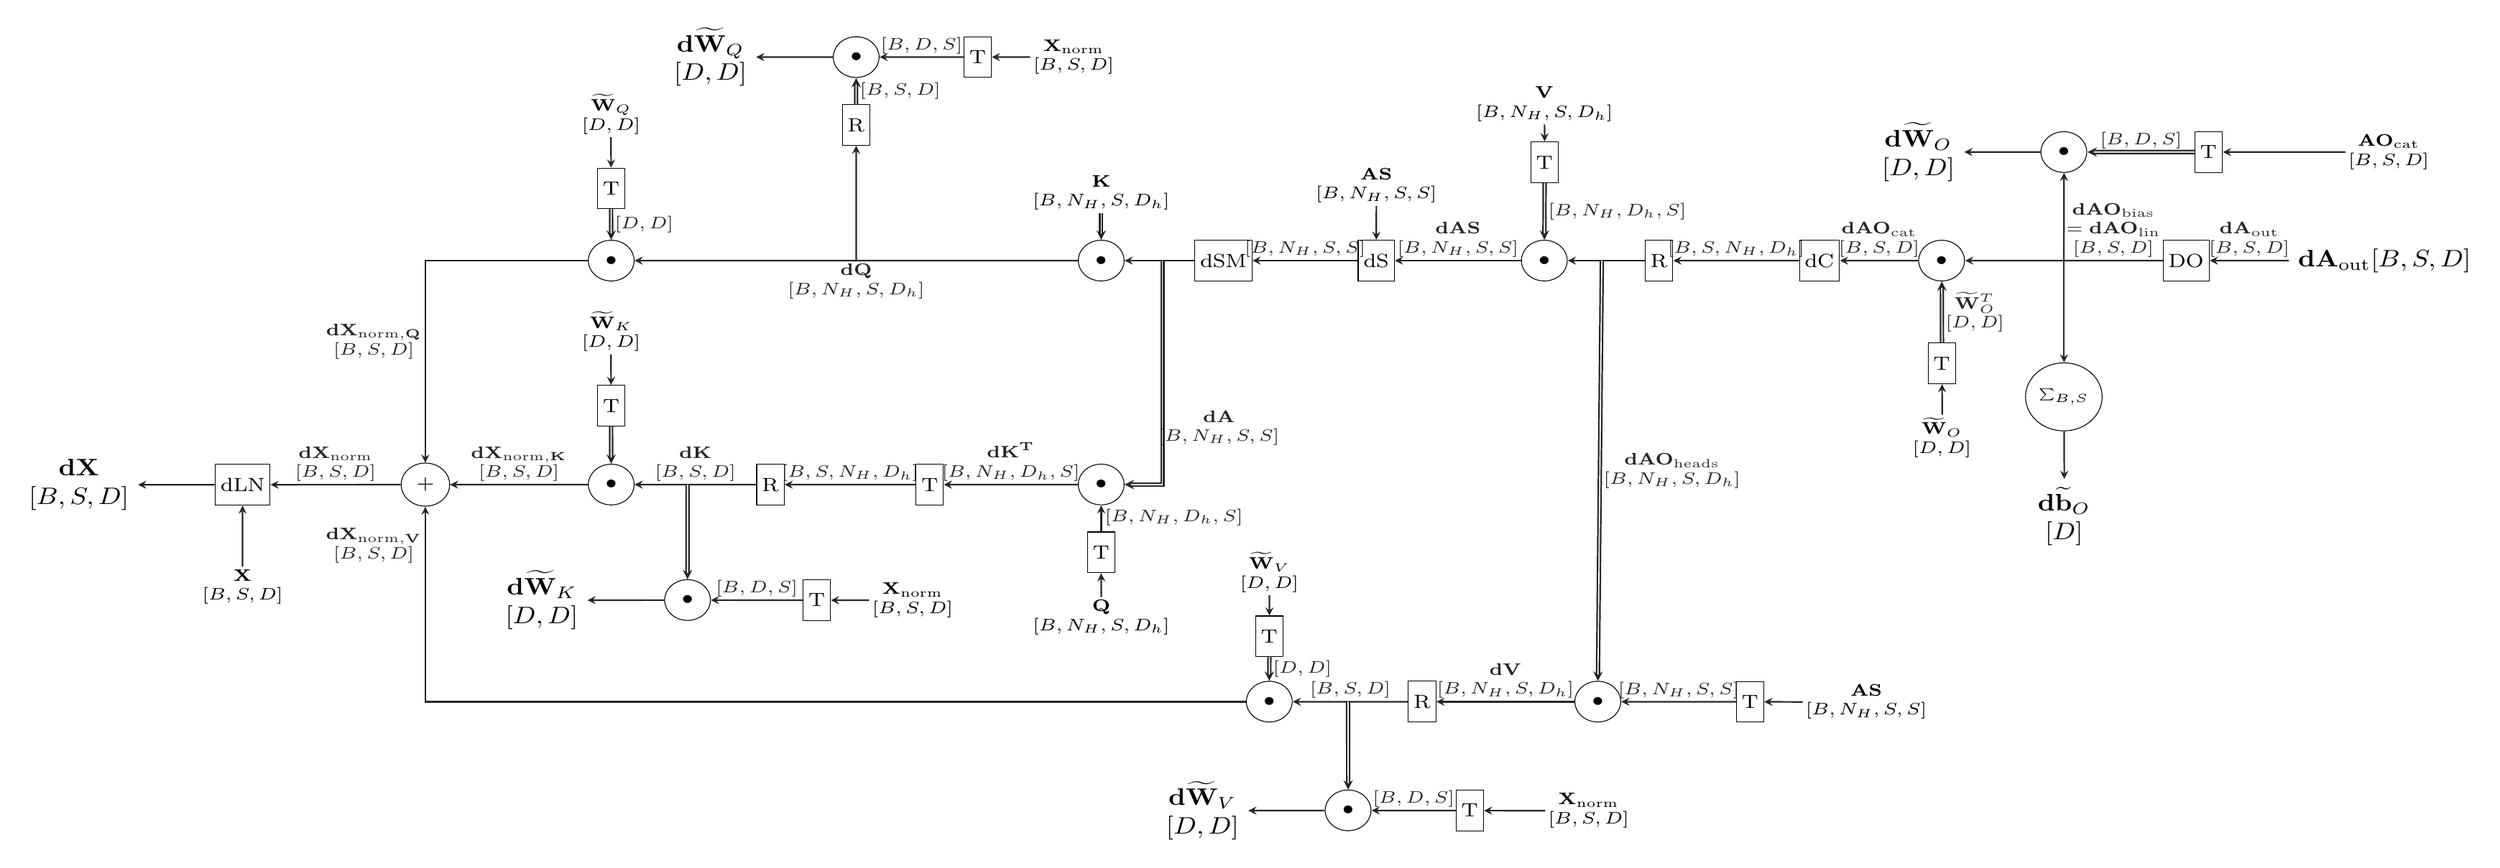
\begin{tikzpicture}[
  every node/.style={transform shape},
  >=stealth,
  auxnode/.style={draw, rectangle, fill=white, minimum height=6mm, inner sep=2pt, font=\footnotesize, align=center},
  mulnode/.style={draw, circle, fill=white, minimum size=6mm, font=\footnotesize, align=center},
  addnode/.style={draw, circle, fill=white, minimum size=6mm, font=\footnotesize, align=center},
  sumnode/.style={draw, circle, fill=white, minimum size=6mm, font=\tiny, align=center},
  flow/.style={->, thick, black!85},
  flow2/.style={->, double, thick, black!85},
  dimlabel/.style={font=\scriptsize, inner sep=1pt, align=center},
  gradflow/.style={->, thick, black!85},
  gradweight/.style={->, thick, black!85}
]

\begin{scope}[xscale=1.35, yscale=1.2]

\def\yoffset{-1.0}
\def\dVXyoffset{-6.5}

\coordinate (Grad_Aout_B) at (17.5, \yoffset);
\coordinate (dDrop_center) at (15.9, \yoffset);
\coordinate (ProjGradSplit) at (14.3, \yoffset);
\coordinate (dOProj_center) at (12.7, \yoffset);
\coordinate (C_center) at (11.1, \yoffset);
\coordinate (R_center) at (9.0, \yoffset);
\coordinate (dPV_AS_calc_center) at (7.5, \yoffset);
\coordinate (dSoft_center) at (5.3, \yoffset);
\coordinate (dSM_calc_center) at (3.3, \yoffset);
\coordinate (dV_calc_center) at (8.2, \dVXyoffset+\yoffset);
\coordinate (R_V_bwd_center) at (5.9, \dVXyoffset+\yoffset);
\coordinate (dVX_calc_center) at (3.9, \dVXyoffset+\yoffset);
\coordinate (dQK_calc_Q_center) at (1.7, \yoffset);
\coordinate (dQK_calc_K_center) at (1.7, -3.3+\yoffset);
\coordinate (K_BWD_input_center) at (1.7, 1.0+\yoffset);
\coordinate (T_Q_bwd_center) at (1.7, -4.3+\yoffset);

% \node[font=\Large\bfseries] at (8, 4.6+\yoffset) {Multi-Head Attention Backward Pass};

\node (Grad_Aout_B) at (18.5, \yoffset) {$\mathbf{dA}_{\text{out}}$\\$[B,S,D]$};
\node[auxnode] (DO) at (dDrop_center) {DO};
\node[mulnode] (dOProj) at (dOProj_center) {$\bullet$};

\node[auxnode] (T_WO) [below=0.9cm of dOProj] {T};
\node[dimlabel] (WO_BWD) [below=0.45cm of T_WO] {$\widetilde{\mathbf{W}}_{O}$\\$[D,D]$};

\node[mulnode] (dWO_calc) at ($(ProjGradSplit)+(0, 1.6)$) {$\bullet$};
\node[align=center, left=1.0cm of dWO_calc]
  (dWO_GRAD) {$\mathbf{d}\widetilde{\mathbf{W}}_{O}$\\$[D,D]$};
\node[auxnode] (T_AO_in) [right=1.4cm of dWO_calc] {T};
\node[dimlabel] (AO_in_local_label) [right=1.6cm of T_AO_in] {$\mathbf{AO}_{\text{cat}}$\\$[B,S,D]$};

\node[auxnode] (C) at (C_center) {dC};
\node[auxnode] (R) at (R_center) {R};

\node[mulnode] (dPV_AS_calc) at (dPV_AS_calc_center) {$\bullet$};
\node[auxnode] (dSoft) at (dSoft_center) {dS};
\node[auxnode] (dSM_calc) at (dSM_calc_center) {dSM};

\node[mulnode] (dQK_calc_Q) at (dQK_calc_Q_center) {$\bullet$};
\node[mulnode] (dQX_proj_calc) [left=5.8cm of dQK_calc_Q] {$\bullet$};

\node[mulnode] (dQK_calc_K) at (dQK_calc_K_center) {$\bullet$};
\node[mulnode] (dKX_proj_calc) [left=5.8cm of dQK_calc_K] {$\bullet$};

\node[dimlabel] (K_BWD_input) at (K_BWD_input_center) {$\mathbf{K}$\\$[B,N_H,S,D_h]$};
\node[auxnode] (T_Q_bwd) at (T_Q_bwd_center) {T};
\node[dimlabel] (Q_BWD_input) [below=0.35cm of T_Q_bwd] {$\mathbf{Q}$\\$[B,N_H,S,D_h]$};

\node[dimlabel] (V_FWD) [above=1.7cm of dPV_AS_calc] {$\mathbf{V}$\\$[B,N_H,S,D_h]$};
\node[auxnode] (T_V_bwd) [below=0.25cm of V_FWD] {T};

\node[mulnode] (dV_calc) at (dV_calc_center) {$\bullet$};
\node[auxnode] (T_AS_bwd) [right=1.5cm of dV_calc] {T};
\node[dimlabel] (AS_BWD_for_V) [right=0.5cm of T_AS_bwd] {$\mathbf{AS}$\\$[B,N_H,S,S]$};

\node[auxnode] (R_V_bwd) at (R_V_bwd_center) {R};
\node[mulnode] (dVX_calc) at (dVX_calc_center) {$\bullet$};

\node[auxnode] (T_WV) [above=0.35cm of dVX_calc] {T};
\node[dimlabel] (WV_BWD) [above=0.3cm of T_WV] {$\widetilde{\mathbf{W}}_{V}$\\$[D,D]$};

\node[sumnode] (Sum_dBO) [below=1.5cm of ProjGradSplit] {$\sum_{B, S}$};
\node (dBO) [align=center, below=0.7cm of Sum_dBO] {$\mathbf{d}\widetilde{\mathbf{b}}_{O}$\\$[D]$};

\draw[gradflow] (Grad_Aout_B) -- (DO)
  node[dimlabel, midway, above]{$\mathbf{dA}_{\text{out}}$\\$[B,S,D]$};

\draw[gradflow] (DO) -- (dOProj)
  node[dimlabel, pos=0.25, above]{$\mathbf{dAO}_{\text{bias}}$\\$=\mathbf{dAO}_{\text{lin}}$\\$[B,S,D]$};

\draw[gradflow] (ProjGradSplit) -- (dWO_calc.south);
\draw[gradflow] (ProjGradSplit) -- ([yshift=-0.75cm]ProjGradSplit) -| (Sum_dBO.north);

\draw[gradflow] (dOProj) -- (C)
  node[dimlabel, midway, above]{$\mathbf{dAO}_{\text{cat}}$\\$[B,S,D]$};
\draw[gradflow] (C) -- (R)
  node[dimlabel, midway, above]{$[B,S,N_H,D_h]$};

\coordinate (R_split_point) at ($(dPV_AS_calc)!0.5!(R)$);
\draw[gradflow] (R.west) -- (dPV_AS_calc.east);
\draw[flow2] (R_split_point) -- (dV_calc.north)
  node[dimlabel, midway, right]{$\mathbf{dAO}_{\text{heads}}$\\$[B,N_H,S,D_h]$};

\draw[gradflow] (V_FWD.south) -- (T_V_bwd.north);
\draw[flow2] (T_V_bwd.south) -- (dPV_AS_calc.north)
  node[dimlabel, midway, right]{$[B,N_H,D_h,S]$};
\draw[gradflow] (dPV_AS_calc.west) -- (dSoft.east)
  node[dimlabel, midway, above]{$\mathbf{dAS}$\\$[B,N_H,S,S]$};

\node (AS_BWD_dS) [dimlabel, above=0.5cm of dSoft] {$\mathbf{AS}$\\$[B,N_H,S,S]$};
\draw[gradflow] (AS_BWD_dS.south) -- (dSoft.north);
\draw[gradflow] (dSoft.west) -- (dSM_calc.east)
  node[dimlabel, midway, above]{$[B,N_H,S,S]$};

\coordinate (dA_Split_X) at ($(dSM_calc_center)!0.5!(dQK_calc_Q_center)$);
\coordinate (dA_Split) at (dA_Split_X |- dQK_calc_Q.east);
\draw[gradflow] (dSM_calc.west) -- (dQK_calc_Q.east);
\draw[flow2] (dA_Split) -- (dA_Split |- dQK_calc_K.east) -- (dQK_calc_K.east)
  node[dimlabel, pos=-1.5, above, yshift=15]{$\mathbf{dA}$\\$[B,N_H,S,S]$};

\draw[flow2] (K_BWD_input.south) -- (dQK_calc_Q.north);
\draw[gradweight] (dQK_calc_Q) -- (dQX_proj_calc)
  node[dimlabel, midway, below]{$\mathbf{dQ}$\\$[B,N_H,S,D_h]$};

\node[auxnode] (T_WQ_bwd) [above=0.45cm of dQX_proj_calc] {T};
\node[dimlabel] (WQ_bwd) [above=0.45cm of T_WQ_bwd] {$\widetilde{\mathbf{W}}_{Q}$\\$[D,D]$};
\draw[flow] (WQ_bwd) -- (T_WQ_bwd);
\draw[flow2] (T_WQ_bwd.south) -- (dQX_proj_calc.north)
  node[dimlabel, midway, right]{$[D,D]$};

\draw[flow] (Q_BWD_input.north) -- (T_Q_bwd.south);
\draw[flow] (T_Q_bwd.north) -- (dQK_calc_K.south)
  node[dimlabel, pos=0.55, right]{$[B,N_H,D_h,S]$};

\node[auxnode] (T_dK) at ($(dQK_calc_K)!0.35!(dKX_proj_calc)$) {T};
\node[auxnode] (R_dK_mid) at ($(T_dK)!0.5!(dKX_proj_calc)$) {R};

\draw[gradweight] (dQK_calc_K) -- (T_dK)
  node[dimlabel, midway, above]{$\mathbf{dK^T}$\\$[B,N_H,D_h,S]$};
\draw[gradweight] (T_dK) -- (R_dK_mid)
  node[dimlabel, midway, above]{$[B,S,N_H,D_h]$};
\draw[gradweight] (R_dK_mid) -- (dKX_proj_calc)
  node[dimlabel, midway, above]{$\mathbf{dK}$\\$[B,S,D]$};

\node[auxnode] (T_WK_bwd) [above=0.55cm of dKX_proj_calc] {T};
\node[dimlabel] (WK_bwd) [above=0.45cm of T_WK_bwd] {$\widetilde{\mathbf{W}}_{K}$\\$[D,D]$};
\draw[gradflow] (WK_bwd) -- (T_WK_bwd);
\draw[flow2] (T_WK_bwd.south) -- (dKX_proj_calc.north);

\draw[gradflow] (AS_BWD_for_V.west) -- (T_AS_bwd.east);
\draw[gradflow] (T_AS_bwd.west) -- (dV_calc.east)
  node[dimlabel, midway, above]{$[B,N_H,S,S]$};
\draw[gradflow] (dV_calc.west) -- (R_V_bwd.east)
  node[dimlabel, midway, above]{$\mathbf{dV}$\\$[B,N_H,S,D_h]$};
\draw[gradflow] (R_V_bwd) -- (dVX_calc.east)
  node[dimlabel, midway, above]{$[B,S,D]$};

\draw[gradflow] (WV_BWD) -- (T_WV);
\draw[flow2] (T_WV) -- (dVX_calc.north)
  node[dimlabel, midway, right]{$[D,D]$};

\node[addnode] (Sum_dXnorm) [left=1.8cm of dKX_proj_calc] {$+$};

\draw[gradweight] (dQX_proj_calc.west) -| node[dimlabel, pos=0.7, left]{$\mathbf{dX}_{\text{norm},\mathbf{Q}}$\\$[B,S,D]$} (Sum_dXnorm.north);
\draw[gradweight] (dKX_proj_calc.west) -- node[dimlabel, midway, above]{$\mathbf{dX}_{\text{norm},\mathbf{K}}$\\$[B,S,D]$} (Sum_dXnorm.east);
\draw[gradweight] (dVX_calc.west) -| node[dimlabel, pos=0.9, left]{$\mathbf{dX}_{\text{norm},\mathbf{V}}$\\$[B,S,D]$} (Sum_dXnorm.south);

\coordinate (dV_branch) at ($(R_V_bwd.west)!0.52!(dVX_calc.east)$);
\node[mulnode] (dWV_mul) at ($(dV_branch)+(0,-1.6cm)$) {$\bullet$};
\draw[flow2] (dV_branch) -- (dWV_mul.north);

\node[auxnode] (T_Xnorm) [right=1.1cm of dWV_mul] {T};
\node[dimlabel] (Xnorm_local) [right=0.8cm of T_Xnorm] {$\mathbf{X}_{\text{norm}}$\\$[B,S,D]$};
\draw[gradflow] (Xnorm_local) -- (T_Xnorm);
\draw[gradflow] (T_Xnorm.west) -- (dWV_mul.east)
  node[dimlabel, midway, above]{$[B,D,S]$};
\node (dWV_out) [align=center, left=1.0cm of dWV_mul] {$\mathbf{d}\widetilde{\mathbf{W}}_{V}$\\$[D,D]$};
\draw[gradweight] (dWV_mul.west) -- (dWV_out);

\coordinate (dQ_branch) at ($(dQK_calc_Q.east)!0.50!(dQX_proj_calc.west)$);
\node[mulnode] (dWQ_mul) at ($(dQ_branch)+(0,3.0cm)$) {$\bullet$};
\node[auxnode] (R_dQ_for_WQ) at ($(dWQ_mul)+(0,-1.0cm)$) {R};
\draw[gradflow]  (dQ_branch) -- (R_dQ_for_WQ.south);
\draw[flow2] (R_dQ_for_WQ.north) -- (dWQ_mul.south)
  node[dimlabel, midway, right]{$[B,S,D]$};

\node[auxnode] (T_XnormQ) [right=1.1cm of dWQ_mul] {T};
\node[dimlabel] (Xnorm_localQ) [right=0.5cm of T_XnormQ] {$\mathbf{X}_{\text{norm}}$\\$[B,S,D]$};
\draw[gradflow] (Xnorm_localQ) -- (T_XnormQ);
\draw[gradflow] (T_XnormQ.west) -- (dWQ_mul.east)
  node[dimlabel, midway, above]{$[B,D,S]$};
\node (dWQ_out) [align=center, left=1.0cm of dWQ_mul] {$\mathbf{d}\widetilde{\mathbf{W}}_{Q}$\\$[D,D]$};
\draw[gradweight] (dWQ_mul.west) -- (dWQ_out);

\coordinate (dK_branch) at ($(R_dK_mid)!0.52!(dKX_proj_calc)$);
\node[mulnode] (dWK_mul) at ($(dK_branch)+(0,-1.7cm)$) {$\bullet$};
\draw[flow2]  (dK_branch) -- (dWK_mul.north);

\node[auxnode] (T_XnormK) [right=1.2cm of dWK_mul] {T};
\node[dimlabel, right=0.5cm of T_XnormK] (Xnorm_localK) {$\mathbf{X}_{\text{norm}}$\\$[B,S,D]$};
\draw[gradflow] (Xnorm_localK) -- (T_XnormK);
\draw[gradflow] (T_XnormK.west) -- (dWK_mul.east)
  node[dimlabel, midway, above]{$[B,D,S]$};
\node (dWK_out) [align=center, left=1.0cm of dWK_mul] {$\mathbf{d}\widetilde{\mathbf{W}}_{K}$\\$[D,D]$};
\draw[gradweight] (dWK_mul.west) -- (dWK_out);

\draw[gradweight] (Sum_dBO) -- (dBO);

\draw[gradflow] (WO_BWD) -- (T_WO);
\draw[flow2] (T_WO) -- (dOProj)
  node[dimlabel, midway, right]{$\widetilde{\mathbf{W}}_{O}^{T}$\\$[D,D]$};
\draw[gradflow] (AO_in_local_label) -- (T_AO_in);
\draw[flow2] (T_AO_in) -- (dWO_calc.east)
  node[dimlabel, midway, above]{$[B,D,S]$};
\draw[gradweight] (dWO_calc) -- (dWO_GRAD);

\node[auxnode] (dLN) [left=1.7cm of Sum_dXnorm] {dLN};
\draw[gradweight] (Sum_dXnorm.west) -- node[dimlabel, midway, above]
  {$\mathbf{dX}_{\text{norm}}$\\$[B,S,D]$} (dLN.east);

\node (dX_OUT) [align=center, left=1.0cm of dLN] {$\mathbf{dX}$\\$[B,S,D]$};
\draw[gradweight] (dLN.west) -- (dX_OUT);

\node[dimlabel] (LNCache) [below=0.9cm of dLN] {$\mathbf{X}$\\$[B,S,D]$};
\draw[gradflow] (LNCache.north) -- (dLN.south);

\end{scope}
\end{tikzpicture}
}

  \caption{단일 노드 MHA 블록의 역전파.
  출력 $\mathbf{A}_{\text{out}}$에 대한 기울기에서 시작하여,
  출력 프로젝션, 어텐션 연산, Q/K/V 선형 레이어, 레이어 정규화를
  역순으로 거치며 입력과 파라미터에 대한 기울기를 계산한다.}
  \label{fig:single_node_mha_backward}
\end{figure}
\end{landscape}


% ------------------------ 5.3 MLP / FFN ------------------------------

\subsection{피드포워드 네트워크 (MLP / FFN)}

트랜스포머 블록의 MLP(또는 FFN) 부분은
각 시퀀스 위치별로 독립적인 비선형 변환을 수행한다.
구조적으로는 두 개의 선형 레이어와 중간 비선형 함수로 이루어져 있으며,
앞에서 정의한
\[
  \mathbf{X}, \mathbf{Y} \in \mathbb{R}^{B \times S \times D}, \quad
  \mathbf{Z}_{\text{up}}, \mathbf{Z}_{\text{act}}
  \in \mathbb{R}^{B \times S \times D_{\text{ff}}}
\]
를 사용한다.

\subsubsection{순전파}

MHA 블록의 출력을 $\mathbf{A}_{\text{out}}$라 두고,
잔차 연결까지 반영된 텐서를 $\mathbf{X}_2$라고 하자
(Section~\ref{sec:background}의 트랜스포머 블록 구조 참조).
MLP 블록에서는 다음과 같은 순서를 따른다.

\paragraph{(1) 레이어 정규화.}
\[
  \mathbf{X}_3 = \mathrm{LN}(\mathbf{X}_2)
  \in \mathbb{R}^{B \times S \times D}.
\]

\paragraph{(2) 상향 선형 레이어 (up-projection).}
\[
  \mathbf{Z}_{\text{up}} = \mathbf{X}_3 W_{\text{up}} + \mathbf{b}_{\text{up}},
\]
여기서 $W_{\text{up}} \in \mathbb{R}^{D \times D_{\text{ff}}}$,
$\mathbf{b}_{\text{up}} \in \mathbb{R}^{D_{\text{ff}}}$이다.

\paragraph{(3) 비선형 활성 함수.}
\[
  \mathbf{Z}_{\text{act}} = \phi(\mathbf{Z}_{\text{up}}),
\]
GELU, ReLU 등 원소별 비선형 함수를 사용한다.

\paragraph{(4) 하향 선형 레이어 (down-projection).}
\[
  \mathbf{H}_{\text{mlp}}
  = \mathbf{Z}_{\text{act}} W_{\text{down}} + \mathbf{b}_{\text{down}},
\]
여기서 $W_{\text{down}} \in \mathbb{R}^{D_{\text{ff}} \times D}$,
$\mathbf{b}_{\text{down}} \in \mathbb{R}^{D}$이다.

\paragraph{(5) 잔차 연결.}
최종적으로 MLP 출력은
\[
  \mathbf{X}_{\text{out}} = \mathbf{X}_2 + \mathbf{H}_{\text{mlp}}
\]
와 같이 잔차 연결을 통해 합쳐진다.

\begin{figure}[htbp]
  \centering
  \resizebox{\linewidth}{!}{%
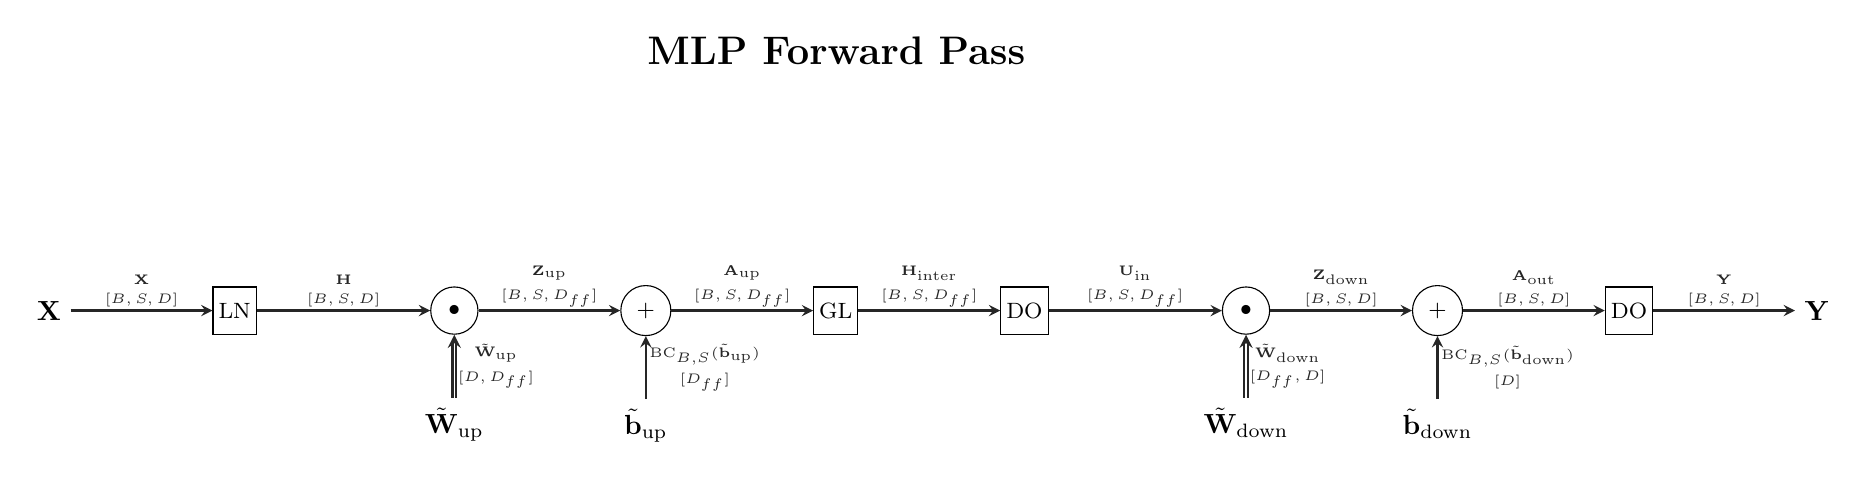
\begin{tikzpicture}[
    >=stealth,
    auxnode/.style={draw, rectangle, fill=white, minimum height=6mm, inner sep=2pt, font=\footnotesize, align=center},
    mulnode/.style={draw, circle, fill=white, minimum size=6mm, font=\footnotesize, align=center},
    addnode/.style={draw, circle, fill=white, minimum size=6mm, font=\footnotesize, align=center},
    sumnode/.style={draw, circle, fill=white, minimum size=6mm, font=\tiny, align=center},
    flow/.style={->, thick, black!85},
    flow2/.style={double, ->, thick, black!85},
    dimlabel/.style={font=\tiny, inner sep=1pt, align=center}
]
    \node[font=\Large\bfseries] at (10, 2.8) {MLP Forward Pass};

    \pgfmathsetmacro{\verticaloffset}{-0.5}

    \node            (MIn)   at (0,\verticaloffset) {$\mathbf{X}$};
    \node[auxnode]   (LN2)   [right=1.8cm of MIn] {LN};
    \node[mulnode]   (L1Mul) [right=2.2cm of LN2] {$\bullet$};
    \node            (Wup)   [below=0.8cm of L1Mul] {$\tilde{\mathbf{W}}_{\text{up}}$};
    \node[addnode]   (AddB1) [right=1.8cm of L1Mul] {+};
    \node            (Bup)   [below=0.8cm of AddB1] {$\tilde{\mathbf{b}}_{\text{up}}$};
    \node[auxnode]   (Act)   [right=1.8cm of AddB1] {GL};
    \node[auxnode]   (Drop1) [right=1.8cm of Act] {DO};
    \node[mulnode]   (L2Mul) [right=2.2cm of Drop1] {$\bullet$};
    \node            (Wdown) [below=0.8cm of L2Mul] {$\tilde{\mathbf{W}}_{\text{down}}$};
    \node[addnode]   (AddB2) [right=1.8cm of L2Mul] {+};
    \node            (Bdown) [below=0.8cm of AddB2] {$\tilde{\mathbf{b}}_{\text{down}}$};
    \node[auxnode]   (Drop2) [right=1.8cm of AddB2] {DO};
    \node            (MOut)  [right=1.8cm of Drop2] {$\mathbf{Y}$};

    \draw[flow] (MIn) -- (LN2) node[dimlabel, midway, above]{\shortstack{$\mathbf{X}$\\$[B,S,D]$}};
    \draw[flow] (LN2) -- (L1Mul) node[dimlabel, midway, above]{\shortstack{$\mathbf{H}$\\$[B,S,D]$}};
    \draw[flow2] (Wup) -- (L1Mul) node[dimlabel, midway, right]{\shortstack{$\tilde{\mathbf{W}}_{\text{up}}$\\$[D, D_{ff}]$}};
    \draw[flow] (L1Mul) -- (AddB1) node[dimlabel, midway, above]{\shortstack{$\mathbf{Z}_{\text{up}}$\\$[B,S,D_{ff}]$}};
    \draw[flow] (Bup) -- (AddB1) node[dimlabel, midway, right]{\shortstack{$\mathrm{BC}_{B,S}(\tilde{\mathbf{b}}_{\text{up}})$\\$[D_{ff}]$}};
    \draw[flow] (AddB1) -- (Act) node[dimlabel, midway, above]{\shortstack{$\mathbf{A}_{\text{up}}$\\$[B,S,D_{ff}]$}};
    \draw[flow] (Act) -- (Drop1) node[dimlabel, midway, above]{\shortstack{$\mathbf{H}_{\text{inter}}$\\$[B,S,D_{ff}]$}};
    \draw[flow] (Drop1) -- (L2Mul) node[dimlabel, midway, above]{\shortstack{$\mathbf{U}_{\text{in}}$\\$[B,S,D_{ff}]$}};
    \draw[flow2] (Wdown) -- (L2Mul) node[dimlabel, midway, right]{\shortstack{$\tilde{\mathbf{W}}_{\text{down}}$\\$[D_{ff}, D]$}};
    \draw[flow] (L2Mul) -- (AddB2) node[dimlabel, midway, above]{\shortstack{$\mathbf{Z}_{\text{down}}$\\$[B,S,D]$}};
    \draw[flow] (Bdown) -- (AddB2) node[dimlabel, midway, right]{\shortstack{$\mathrm{BC}_{B,S}(\tilde{\mathbf{b}}_{\text{down}})$\\$[D]$}};
    \draw[flow] (AddB2) -- (Drop2) node[dimlabel, midway, above]{\shortstack{$\mathbf{A}_{\text{out}}$\\$[B,S,D]$}};
    \draw[flow] (Drop2) -- (MOut) node[dimlabel, midway, above]{\shortstack{$\mathbf{Y}$\\$[B,S,D]$}};

\end{tikzpicture}%
}

  \caption{단일 노드 MLP/FFN 블록의 순전파.
  입력 $\mathbf{X}_2$는 레이어 정규화를 거쳐 상향 선형 레이어,
  비선형 활성 함수, 하향 선형 레이어를 통과한 뒤,
  잔차 연결을 통해 $\mathbf{X}_{\text{out}}$을 형성한다.}
  \label{fig:single_node_mlp_forward}
\end{figure}

\subsubsection{역전파}

역전파에서는 $\mathrm{d}\mathbf{X}_{\text{out}}$에서 시작하여
잔차 연결을 통해 $\mathrm{d}\mathbf{X}_2$와
$\mathrm{d}\mathbf{H}_{\text{mlp}}$를 얻고,
이후 각 선형 레이어와 비선형 함수, 레이어 정규화를
역순으로 따라가며 기울기를 계산한다.

구체적으로는 다음과 같은 단계로 이해할 수 있다.
\begin{itemize}
  \item 잔차 연결 역전파: $\mathrm{d}\mathbf{X}_2$와
        $\mathrm{d}\mathbf{H}_{\text{mlp}}$가 동일한 기울기를 받는다.
  \item 하향 선형 레이어 역전파를 통해
        $\mathrm{d}\mathbf{Z}_{\text{act}}$, $W_{\text{down}}$과
        $\mathbf{b}_{\text{down}}$에 대한 기울기를 계산한다.
  \item 비선형 함수 역전파를 통해 $\mathrm{d}\mathbf{Z}_{\text{up}}$를 얻는다.
  \item 상향 선형 레이어 역전파를 통해
        $\mathrm{d}\mathbf{X}_3$, $W_{\text{up}}$과
        $\mathbf{b}_{\text{up}}$에 대한 기울기를 계산한다.
  \item 마지막으로 레이어 정규화 역전파를 통해
        $\mathrm{d}\mathbf{X}_2$를 입력 방향으로 전파한다.
\end{itemize}

\begin{figure}[htbp]
  \centering
  \noindent
\resizebox{\linewidth}{!}{%
\begin{tikzpicture}[
    >=stealth,
    auxnode/.style={draw, rectangle, fill=white, minimum height=6mm, inner sep=2pt, font=\footnotesize, align=center},
    mulnode/.style={draw, circle, fill=white, minimum size=6mm, font=\footnotesize, align=center},
    addnode/.style={draw, circle, fill=white, minimum size=6mm, font=\footnotesize, align=center},
    sumnode/.style={draw, circle, fill=white, minimum size=6mm, font=\tiny, align=center},
    flow_rev/.style={<-, thick, black!85},
    flow_dw/.style={->, thick, black!85},
    flow_act/.style={double, ->, thick, black!85},
    dimlabel/.style={font=\tiny, inner sep=1pt, align=center},
    gradlabel/.style={font=\tiny\bfseries, inner sep=1pt, align=center}
]
    \node[font=\Large\bfseries] at (5, 10) {MLP Backward Pass};

    \pgfmathsetmacro{\backwardoffset}{0.0}

    \node (d_MOut) at (12.6, \backwardoffset) {$\mathrm{d}\mathbf{Y}$};
    \node[auxnode] (d_Drop2) [left=1.8cm of d_MOut] {dDO};
    \draw[flow_rev] (d_Drop2) -- (d_MOut)
      node[dimlabel, midway, below]{\shortstack{$\mathrm{d}\mathbf{Y}$\\$[B,S,D]$}};

    \coordinate (split2) at ($(d_Drop2.west) + (-1.5cm, 0)$);
    \coordinate (branch_dUproj) at ($(split2) + (-1.2cm, 0)$);

    \node[sumnode] (d_SumB2) [above=0.8cm of split2] {$\sum_{B, S}$};
    \node (d_Bdown) [above=0.8cm of d_SumB2] {$\mathrm{d}\tilde{\mathbf{b}}_{\text{down}}$};
    \draw[flow_dw] (d_SumB2) -- (d_Bdown) node[dimlabel, midway, right]{$[D]$};

    \draw[flow_rev] (split2) -- (d_Drop2);
    \draw[flow_rev] (d_SumB2) -- (split2);

    \node[mulnode] (d_L2Mul_in) [left=2.2cm of split2] {$\bullet$};
    \draw[flow_rev] (d_L2Mul_in) -- (d_Drop2)
      node[gradlabel, midway, below]{\shortstack{$\mathrm{d}\mathbf{Z}_{\text{down}}=\mathrm{d}\mathbf{A}_{\text{out}}$\\$[B,S,D]$}};

    \node (W_down_T) [below=1.8cm of d_L2Mul_in] {$\tilde{\mathbf{W}}_{\text{down}}^{T}$};
    \draw[flow_act] (W_down_T.north) -- (d_L2Mul_in)
      node[dimlabel, midway, right]{$[D, D_{ff}]$};

    \coordinate (L2Mul_w_y) at ($(d_L2Mul_in) + (0, 3.5cm)$);
    \node[mulnode] (d_L2Mul_w) at (L2Mul_w_y) {$\bullet$};
    \node (d_Wdown) [above=0.8cm of d_L2Mul_w] {$\mathrm{d}\tilde{\mathbf{W}}_{\text{down}}$};
    \draw[flow_dw] (d_L2Mul_w) -- (d_Wdown) node[dimlabel, midway, right]{$[D_{ff}, D]$};

    \draw[flow_act] (branch_dUproj.north) |- (d_L2Mul_w.east);

    \node[auxnode] (Uin_T) at ($(d_L2Mul_w.west) + (-1.5cm, 0)$) {T};
    \draw[flow_dw] (Uin_T) -- (d_L2Mul_w)
      node[dimlabel, midway, below]{\shortstack{$\mathbf{U}_{\text{in}}^T$\\$[B, D_{ff}, S]$}};
    \node (Uin_aux) [left=1.8cm of Uin_T] {$\mathbf{U}_{\text{in}}$};
    \draw[flow_dw] (Uin_aux) -- (Uin_T) node[dimlabel, midway, above]{\shortstack{$[B,S,D_{ff}]$}};

    \node[auxnode] (d_Drop1) [left=1.8cm of d_L2Mul_in] {dDO};
    \draw[flow_rev] (d_Drop1) -- (d_L2Mul_in)
      node[dimlabel, midway, below]{\shortstack{$\mathrm{d}\mathbf{U}_{\text{in}}$\\$[B,S,D_{ff}]$}};

    \node[auxnode] (d_Act) [left=1.8cm of d_Drop1] {dGL};
    \draw[flow_rev] (d_Act) -- (d_Drop1)
      node[dimlabel, midway, below]{\shortstack{$\mathrm{d}\mathbf{H}_{\text{inter}}$\\$[B,S,D_{ff}]$}};

    \coordinate (split1) at ($(d_Act.west) + (-1.5cm, 0)$);
    \coordinate (branch_dHpre) at ($(split1) + (-1.2cm, 0)$);

    \node[sumnode] (d_SumB1) [above=0.8cm of split1] {$\sum_{B, S}$};
    \node (d_Bup) [above=0.8cm of d_SumB1] {$\mathrm{d}\tilde{\mathbf{b}}_{\text{up}}$};
    \draw[flow_dw] (d_SumB1) -- (d_Bup) node[dimlabel, midway, right]{$[D_{ff}]$};

    \draw[flow_rev] (split1) -- (d_Act);
    \draw[flow_rev] (d_SumB1) -- (split1);

    \node[mulnode] (d_L1Mul_in) [left=2.2cm of split1] {$\bullet$};
    \draw[flow_rev] (d_L1Mul_in) -- (d_Act)
      node[gradlabel, midway, below]{\shortstack{$\mathrm{d}\mathbf{Z}_{\text{up}}=\mathrm{d}\mathbf{A}_{\text{up}}$\\$[B,S,D_{ff}]$}};

    \node (W_up_T) [below=1.8cm of d_L1Mul_in] {$\tilde{\mathbf{W}}_{\text{up}}^{T}$};
    \draw[flow_act] (W_up_T.north) -- (d_L1Mul_in)
      node[dimlabel, midway, right]{$[D_{ff}, D]$};

    \coordinate (L1Mul_w_y) at ($(d_L1Mul_in) + (0, 3.5cm)$);
    \node[mulnode] (d_L1Mul_w) at (L1Mul_w_y) {$\bullet$};
    \node (d_Wup) [above=0.8cm of d_L1Mul_w] {$\mathrm{d}\tilde{\mathbf{W}}_{\text{up}}$};
    \draw[flow_dw] (d_L1Mul_w) -- (d_Wup) node[dimlabel, midway, right]{$[D, D_{ff}]$};

    \draw[flow_act] (branch_dHpre.north) |- (d_L1Mul_w.east);

    \node[auxnode] (Znorm_T) at ($(d_L1Mul_w.west) + (-1.5cm, 0)$) {T};
    \draw[flow_dw] (Znorm_T) -- (d_L1Mul_w)
      node[dimlabel, midway, below]{\shortstack{$\mathbf{H}^T$\\$[B, D, S]$}};
    \node (Znorm_aux) [left=1.8cm of Znorm_T] {$\mathbf{H}$};
    \draw[flow_dw] (Znorm_aux) -- (Znorm_T) node[dimlabel, midway, above]{\shortstack{$[B,S,D]$}};

    \node[auxnode] (d_LN2) [left=1.8cm of d_L1Mul_in] {dLN};
    \draw[flow_rev] (d_LN2) -- (d_L1Mul_in)
      node[dimlabel, midway, below]{\shortstack{$\mathrm{d}\mathbf{H}$\\$[B,S,D]$}};

    \node (d_MIn) [left=1.8cm of d_LN2] {$\mathrm{d}\mathbf{X}$};
    \draw[flow_rev] (d_MIn) -- (d_LN2)
      node[dimlabel, midway, below]{\shortstack{$\mathrm{d}\mathbf{X}$\\$[B,S,D]$}};
\end{tikzpicture}%
}

  \caption{단일 노드 MLP/FFN 블록의 역전파.
  잔차 연결, 하향/상향 선형 레이어, 비선형 함수, 레이어 정규화를
  역순으로 통과하며, 각 입력과 파라미터에 대한 기울기를 계산한다.}
  \label{fig:single_node_mlp_backward}
\end{figure}


% ------------------------ 5.4 Output Projection and Loss -------------

\subsection{출력 프로젝션과 손실}

마지막으로, 트랜스포머 레이어의 출력
$\mathbf{X}_{\text{out}} \in \mathbb{R}^{B \times S \times D}$에서
언어 모델 로그릿(logits)을 만들고, 손실을 계산하는 부분을 살펴본다.
여기서는 언어 모델링 또는 다음 토큰 예측을 위한
전형적인 설정을 가정한다.

출력 프로젝션은 언어 모델 행렬 $W_{\text{lm}} \in \mathbb{R}^{D \times V}$
및 bias $\mathbf{b}_{\text{lm}} \in \mathbb{R}^{V}$를 사용하여,
각 위치마다 어휘 크기 $V$에 대한 로그릿을 생성한다.
\[
  \mathbf{Z}_{\text{lm}}[b,s,:]
  = \mathbf{X}_{\text{out}}[b,s,:]\, W_{\text{lm}} + \mathbf{b}_{\text{lm}}.
\]
손실은 보통 소프트맥스-교차 엔트로피(softmax-cross-entropy)로 정의된다.

\subsubsection{순전파 (로그릿, 소프트맥스, 손실)}

순전파는 개념적으로 다음과 같은 단계를 따른다.
\begin{itemize}
  \item $\mathbf{X}_{\text{out}}$에 선형 레이어를 적용하여
        로그릿 텐서 $\mathbf{Z}_{\text{lm}} \in \mathbb{R}^{B \times S \times V}$를 얻는다.
  \item 각 위치별로 소프트맥스를 적용하여 확률 분포를 계산한다.
  \item 목표 토큰(예: 다음 토큰)의 원-핫(one-hot) 벡터와 로그릿을 사용해
        교차 엔트로피 손실을 계산하고, 전체 배치/시퀀스에 대해 평균(또는 합)을 취한다.
\end{itemize}

\begin{figure}[htbp]
  \centering
  
\noindent
\resizebox{\linewidth}{!}{%
\begin{tikzpicture}[
  >=stealth,
  auxnode/.style={draw, rectangle, fill=white, minimum height=6mm, inner sep=2pt, font=\footnotesize, align=center},
  mulnode/.style={draw, circle, fill=white, minimum size=6mm, font=\footnotesize, align=center},
  addnode/.style={draw, circle, fill=white, minimum size=6mm, font=\footnotesize, align=center},
  sumnode/.style={draw, circle, fill=white, minimum size=6mm, font=\tiny, align=center},
  flow/.style={->, thick, black!85},
  flow2/.style={double, ->, thick, black!85},
  dimlabel/.style={font=\tiny, inner sep=1pt, align=center}
]

% From Transformer output
\node            (H)     at (0,-2) {$\mathbf{A}_{\text{out}}$};

% LM head
\node[mulnode]   (LMmul) [right=2.2cm of H] {$\bullet$};
\node            (Wlm)   [align=center, below=0.9cm of LMmul] {$\widetilde{\mathbf{W}}_{\text{lm}}$\\$=\mathbf{E}^{T}$};
\node[addnode]   (AddB)  [right=1.8cm of LMmul] {+};
\node            (blm)   [below=0.9cm of AddB] {$\widetilde{\mathbf{b}}_{\text{lm}}$};

% Softmax → Prob
\node[auxnode]   (SM)    [right=1.8cm of AddB] {S};

\node[auxnode] (ARG)  [right=4.0cm of SM] {ARG};
% Midpoint of SM→P edge (for CE tap)
\coordinate (MidSP) at ($(SM)!0.5!(ARG)$);

% CE node placed below the SM→P edge
\node[auxnode]   (CE)    [below=1.6cm of MidSP] {CE};
\node            (Y)     [right=0.9cm of CE] {$\mathbf{Y_\text{targets}}$};
\node            (Loss)  [align=center, below=1.8cm of CE] {$\mathcal{L}$\\ (mean over $B,S$)};

% Flows
\draw[flow]  (H) -- (LMmul) node[dimlabel, midway, above]{\shortstack{$[B,S,D]$}};
\draw[flow2] (Wlm) -- (LMmul) node[dimlabel, midway, right]{\shortstack{$[D,V]$}};
\draw[flow]  (LMmul) -- (AddB) node[dimlabel, midway, above]{\shortstack{$\mathbf{Z}_{\text{lin}}$\\$[B,S,V]$}};
\draw[flow]  (blm) -- (AddB)   node[dimlabel, midway, right]{\shortstack{$\text{BC}_{B,S}(\widetilde{\mathbf{b}}_{\text{lm}})$\\$[V]$}};
\draw[flow]  (AddB) -- (SM)    node[dimlabel, midway, above]{\shortstack{\textbf{Z\textsubscript{bias}}\\ $[B,S,V]$}};

% Tap the SM→P edge downward into CE
\draw[flow]  (MidSP) -- (CE);
% Targets into CE
\draw[flow]  (Y) -- (CE)  node[dimlabel, midway, above]{\shortstack{targets\\$[B,S]$}};
% Loss goes WEST (left) from CE
\draw[flow]  (CE) -- (Loss);

\node (YhatG) [right=1.8cm of ARG] {$\hat{\mathbf{Y}}_{\text{greedy}}$};
\draw[flow] (SM) -- (ARG)
  node[dimlabel, pos=0.35, above]{\shortstack{$\mathbf{P}$\\$[B,S,V]$}};
\draw[flow] (ARG) -- (YhatG)
  node[dimlabel, midway, above]{\shortstack{token ids\\$[B,S]$}};

% Optional: top-k (or nucleus) sampling path
\node[auxnode] (TopK) [above=1.4cm of ARG] {TOP-$k$};
\node          (YhatS) [right=1.8cm of TopK] {$\hat{\mathbf{Y}}_{\text{sample}}$};
\draw[flow] (MidSP) |- (TopK);
\draw[flow] (TopK) -- (YhatS)
  node[dimlabel, midway, above]{\shortstack{token ids\\$[B,S]$}};

\node[font=\large\bfseries] at (9.2,1.8) {Token Generation \& Loss (Forward)};
\end{tikzpicture}%
}

  \caption{출력 프로젝션과 손실의 순전파.
  은닉 상태 $\mathbf{X}_{\text{out}}$는 언어 모델 프로젝션
  $(W_{\text{lm}}, \mathbf{b}_{\text{lm}})$을 통해 로그릿으로 변환되고,
  소프트맥스와 교차 엔트로피를 거쳐 스칼라 손실 $\mathcal{L}$이 계산된다.}
  \label{fig:single_node_output_forward}
\end{figure}

\subsubsection{역전파}

역전파에서는 손실 $\mathcal{L}$로부터 시작하여,
소프트맥스와 교차 엔트로피를 통합한 형태의 기울기가
로그릿 $\mathbf{Z}_{\text{lm}}$에 대해 계산된다.
실제로는 소프트맥스와 교차 엔트로피의 역전파가 하나의
간단한 표현으로 합쳐지는 경우가 많다.

그 다음 단계는 다음과 같다.
\begin{itemize}
  \item 로그릿에 대한 기울기 $\mathrm{d}\mathbf{Z}_{\text{lm}}$를
        출력 프로젝션 선형 레이어를 통해 역전파하여,
        $\mathrm{d}\mathbf{X}_{\text{out}}$와
        $\mathrm{d}W_{\text{lm}}, \mathrm{d}\mathbf{b}_{\text{lm}}$을 얻는다.
  \item $\mathrm{d}\mathbf{X}_{\text{out}}$는 다시 이전 MLP/FFN 블록과
        MHA, 임베딩 레이어로 전달된다
        (Figure~\ref{fig:single_node_overall} 참고).
\end{itemize}

\begin{figure}[htbp]
  \centering
  \noindent
\resizebox{0.8\linewidth}{!}{%
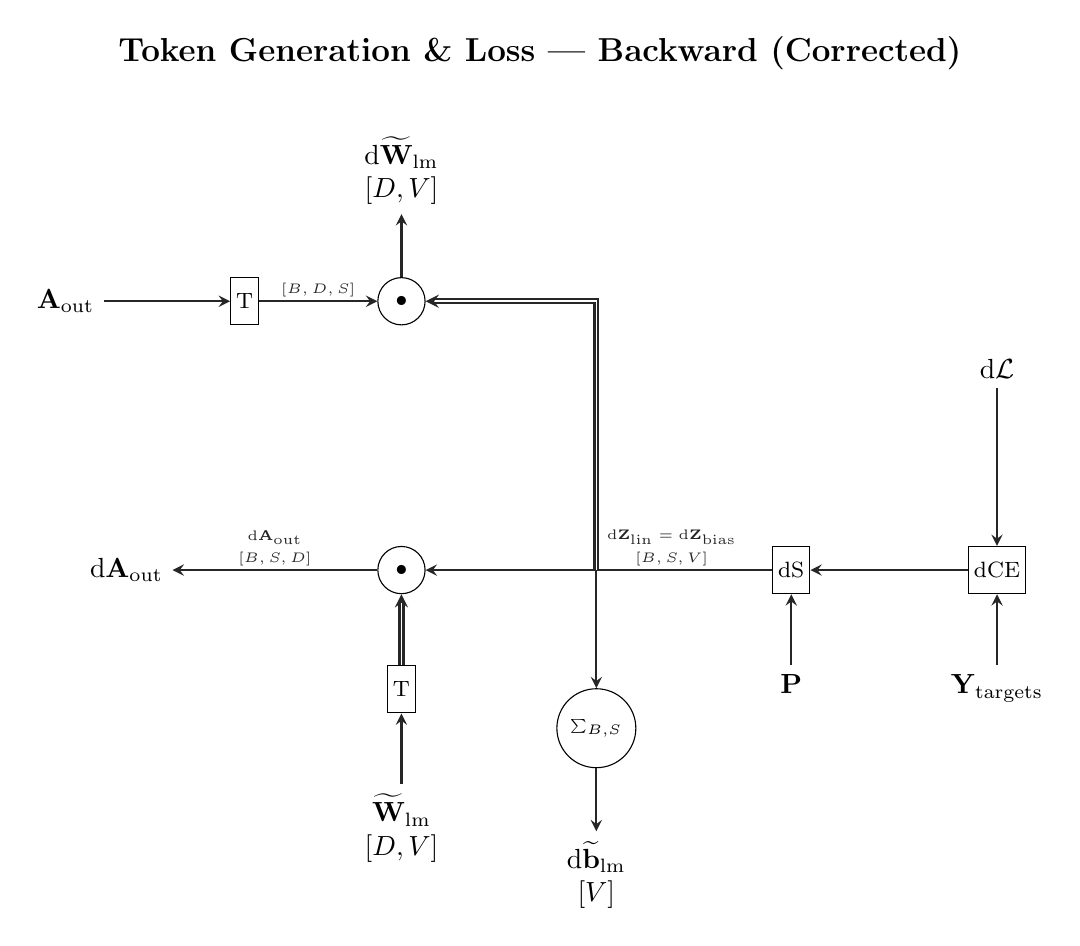
\begin{tikzpicture}[
  >=stealth,
  auxnode/.style={draw, rectangle, fill=white, minimum height=6mm, inner sep=2pt, font=\footnotesize, align=center},
  mulnode/.style={draw, circle, fill=white, minimum size=6mm, font=\footnotesize, align=center},
  addnode/.style={draw, circle, fill=white, minimum size=6mm, font=\footnotesize, align=center},
  sumnode/.style={draw, circle, fill=white, minimum size=6mm, font=\tiny, align=center},
  flow/.style={<-, thick, black!85},
  flow2/.style={double, <-, thick, black!85},
  fwd/.style={->, thick, black!85},
  gradflow/.style={->, thick, black!85},
  dimlabel/.style={font=\tiny, inner sep=1pt, align=center}
]

% Start from dL
\node           (dL)    at (18,0) {$\text{d}\mathcal{L}$};
\node[auxnode]  (dCE)   [below=2.0cm of dL] {dCE};
\node           (Y)     [below=0.9cm of dCE] {$\mathbf{Y_\text{targets}}$};

% Softmax backward
\node[auxnode]  (dS)   [left=2.0cm of dCE] {dS};
\node           (P)     [below=0.9cm of dS] {$\mathbf{P}$};

% Logits (Linear Projection) backprop node
\node[mulnode]  (backMul) [left=4.4cm of dS] {$\bullet$};
\node[auxnode]  (T_Wlm)   [below=0.9cm of backMul] {T};
\node           (Wlm)     [align=center, below=0.9cm of T_Wlm] {$\widetilde{\mathbf{W}}_{\text{lm}}$\\$[D,V]$};

\coordinate (B_split) at ($(backMul)!0.5!(dS)$);

% SUM node for Bias gradient
\node[sumnode]  (SumB) [below=1.5cm of B_split] {$\sum_{B,S}$};
\node           (db)   [align=center, below=0.8cm of SumB] {$\text{d}\widetilde{\mathbf{b}}_{\text{lm}}$\\$[V]$};

% dW calc
\node[mulnode]  (dWmul) [above=2.8cm of backMul] {$\bullet$};
\node[auxnode]  (TAout) [left=1.5cm of dWmul] {T};
\node           (Aout)  [left=1.6cm of TAout] {$\mathbf{A}_{\text{out}}$};
\node           (dW)    [align=center, above=0.8cm of dWmul] {$\text{d}\widetilde{\mathbf{W}}_{\text{lm}}$\\$[D,V]$};

% Back to Transformer
\node           (dH)    [left=2.6cm of backMul] {$\text{d}\mathbf{A}_{\text{out}}$};

% Flows
\draw[flow] (dCE) -- (dL);
\draw[fwd]  (Y) -- (dCE);
\draw[flow] (dS) -- (dCE);
\draw[fwd]  (P) -- (dS);

% Bias grad
\draw[gradflow] (B_split) -- (SumB.north);
\draw[gradflow] (SumB) -- (db);

% Linear projection backprop
\draw[flow] (backMul) -- (dS)
  node[dimlabel, pos=0.71, above]{\shortstack{$\text{d}\mathbf{Z}_{\text{lin}}=\text{d}\mathbf{Z}_{\text{bias}}$\\$[B,S,V]$}};
\draw[flow2] (backMul) -- (T_Wlm);
\draw[fwd]   (Wlm) -- (T_Wlm);
\draw[flow]  (dH) -- (backMul) node[dimlabel, midway, above]{\shortstack{$\text{d}\mathbf{A}_{\text{out}}$\\$[B,S,D]$}};

% dW calculation
\draw[gradflow] (dWmul) -- (dW);
\draw[fwd]  (Aout) -- (TAout);
\draw[fwd]  (TAout) -- (dWmul) node[dimlabel, midway, above]{\shortstack{$[B,D,S]$}};
\draw[flow2] (dWmul) -| (B_split);

\node[font=\large\bfseries, anchor=south]
  at ([yshift=6mm]current bounding box.north) {Token Generation \& Loss — Backward (Corrected)};
\end{tikzpicture}%
}

  \caption{출력 프로젝션과 손실의 역전파.
  손실로부터의 기울기는 소프트맥스와 교차 엔트로피를 거쳐
  로그릿으로 전달되고, 다시 언어 모델 프로젝션을 통해
  $\mathrm{d}\mathbf{A}_{\text{out}}$과
  파라미터 기울기 $\mathrm{d}\mathbf{W}_{\text{lm}}$,
  $\mathrm{d}\mathbf{b}_{\text{lm}}$를 만들어 낸다.}
  \label{fig:single_node_output_backward}
\end{figure}

\else
  % ==========================================================
% 5. Single-Node Transformer: Forward and Backward
% ==========================================================
\section{Single-Node Transformer: Forward and Backward}
\label{sec:sn}

This section presents the full Transformer layer running on a single node
(no parallelism). We emphasize tensor shapes and data flow for both
forward and backward passes. Each subsection covers one major component:

\begin{itemize}
  \item \textbf{Input Embedding}: Converting token IDs to dense vectors.
  \item \textbf{Multi-Head Attention (MHA)}: Computing attention over the sequence.
  \item \textbf{Feed-Forward Network (MLP/FFN)}: Position-wise non-linear processing.
  \item \textbf{Output Projection and Loss}: Generating predictions and computing loss.
\end{itemize}

We assume a batch of tokenized sequences with shape $[B,S]$, where $B$ is
batch size and $S$ is sequence length. The hidden representations inside
the layer typically have shape $[B,S,D]$, where $D$ is the model (hidden)
dimension. In the backward pass we track how gradients with respect to the
scalar loss $\mathcal{L}$ flow backward through these tensors and the
corresponding weight matrices.

% ------------------------ 5.0 Overall Layer Flow ---------------------
\subsection{Overall Transformer Layer Flow}

Before diving into individual components, we provide a high-level view of
how data flows through the entire Transformer layer in both forward and
backward passes. Figure~\ref{fig:single_node_overall} summarizes the
forward path from input embeddings through MHA, MLP, and output projection,
and the corresponding backward paths from the loss back to the embeddings.

\begin{figure}[htbp]
  \centering
  \resizebox{\linewidth}{!}{%
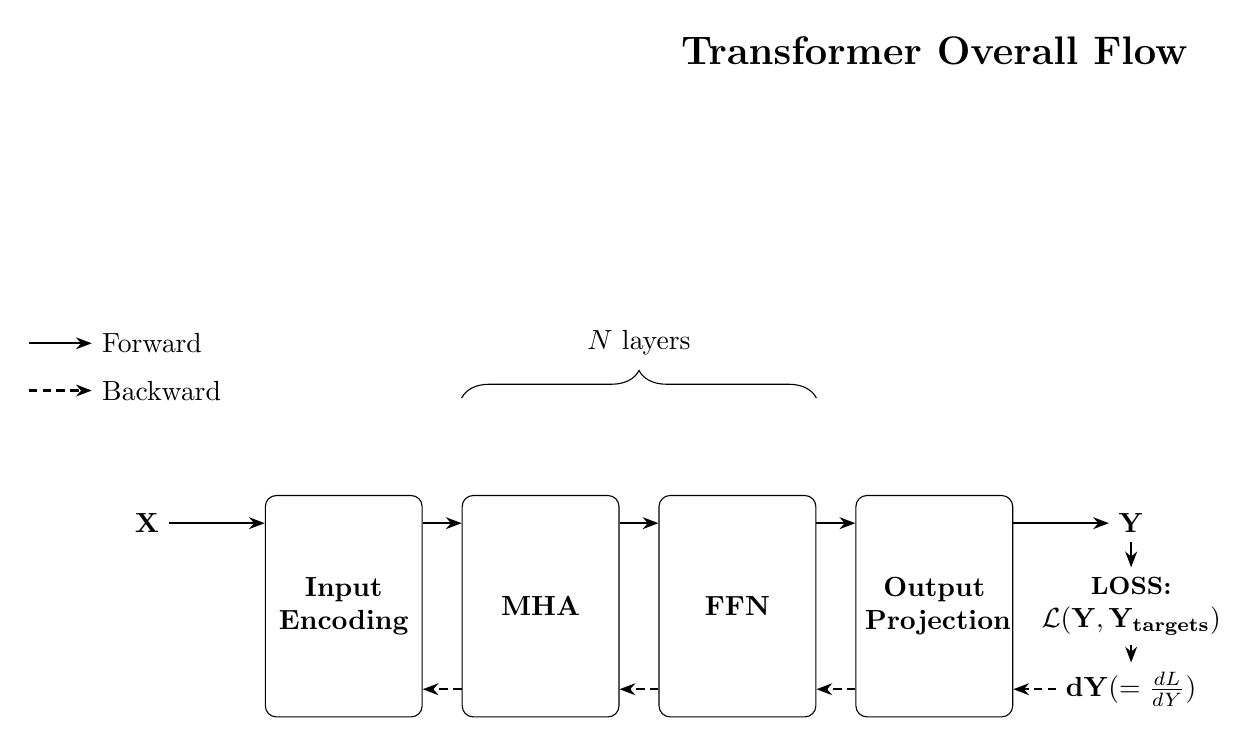
\begin{tikzpicture}[
    node distance=2.5cm,
    >=stealth,
    block/.style={rectangle, draw=black, fill=white, text width=5em, text centered, rounded corners, minimum height=8em, font=\bfseries},
    forward/.style={-{Stealth[length=2mm]}, thick, black},
    backward/.style={-{Stealth[length=2mm]}, thick, black, densely dashed},
    io/.style={text centered, font=\bfseries}
]
    % Title
    \node[font=\Large\bfseries] at (10, 6) {Transformer Overall Flow};

    % Forward path nodes (horizontal)
    \node (input) [io] {$\mathbf{X}$};
    \node (encoding) [block, right of=input, yshift=-3em] {Input\\Encoding};
    \node (mha) [block, right of=encoding] {MHA};
    \node (mlp) [block, right of=mha] {FFN};
    \node (output) [block, right of=mlp] {Output\\Projection};
    \node (pred) [io, right of=output, yshift=3em] {$\mathbf{Y}$};
    \node (loss) [align=center, io, right of=output] {\small LOSS:\\$\mathcal{L}(\mathbf{Y,Y_\text{targets}})$};
    \node (gradient) [io, right of=output, yshift=-3em] {$\mathbf{dY}(=\frac{dL}{dY})$};

    % Forward arrows (upper part of blocks)
    \draw [forward] (input) -- ([yshift=3em]encoding.west);
    \draw [forward] ([yshift=3em]encoding.east) -- ([yshift=3em]mha.west);
    \draw [forward] ([yshift=3em]mha.east) -- ([yshift=3em]mlp.west);
    \draw [forward] ([yshift=3em]mlp.east) -- ([yshift=3em]output.west);
    \draw [forward] ([yshift=3em]output.east) -- (pred);
    \draw [forward] (pred) -- (loss);
    \draw [backward] (loss) -- (gradient);

    % Backward arrows (lower part of blocks)
    \draw [backward] (gradient) -- ([yshift=-3em]output.east);
    \draw [backward] ([yshift=-3em]output.west) -- ([yshift=-3em]mlp.east);
    \draw [backward] ([yshift=-3em]mlp.west) -- ([yshift=-3em]mha.east);
    \draw [backward] ([yshift=-3em]mha.west) -- ([yshift=-3em]encoding.east);

    % Brace for layer repetition
    \draw[decorate, decoration={brace, amplitude=10pt}]
        ([yshift=3.5em]mha.north west) -- ([yshift=3.5em]mlp.north east)
        node[midway, above=12pt, font=\normalsize] {$N$ layers};

    % Labels (Legend)
    \coordinate (legend) at ([xshift=-1.5cm, yshift=6.5em]input);
    \draw[forward] (legend) -- ++(0.8,0) node[right, font=\normalsize] {Forward};
    \draw[backward] ([yshift=-0.6cm]legend) -- ++(0.8,0) node[right, font=\normalsize] {Backward};

\end{tikzpicture}%
}
  \caption{Single-node Transformer layer: overall forward and backward
  flow. Solid arrows denote forward activations, and dashed arrows denote
  gradients flowing backward from the loss $\mathcal{L}$ through the
  output projection, MLP, MHA, and back to the input embeddings.}
  \label{fig:single_node_overall}
\end{figure}


% ------------------------ 5.1 Input Embedding ------------------------
\subsection{Input Embedding Layer}

The input embedding layer converts discrete token IDs into continuous
vector representations, producing the initial hidden states
$\mathbf{X} \in \mathbb{R}^{B \times S \times D}$ that enter the
Transformer stack. We assume:

\begin{itemize}
  \item A token embedding matrix $\mathbf{E} \in \mathbb{R}^{V \times D}$,
        where $V$ is the vocabulary size.
  \item A positional embedding table $\mathbf{P} \in \mathbb{R}^{S \times D}$,
        either learned or fixed (e.g., sinusoidal).
\end{itemize}

Given token IDs $\mathbf{T} \in [B,S]$, the embedding layer performs:

\begin{enumerate}
  \item \textbf{Token embedding lookup}: each token ID indexes into
        $\mathbf{E}$ to form $\mathbf{X}_{\text{tok}} \in [B,S,D]$.
  \item \textbf{Positional embedding addition}: positional vectors
        $\mathbf{P}[s,:]$ are added to each time step $s$.
  \item \textbf{Dropout (optional)}: a dropout layer may be applied to
        the resulting embeddings for regularization during training.
\end{enumerate}

The resulting hidden states $\mathbf{X}$, with shape $[B,S,D]$, appear on
the left of Figure~\ref{fig:single_node_overall} as the starting point of
the layer, and the detailed dataflow inside the embedding block is shown
in Figure~\ref{fig:single_node_input_embedding}.

\subsubsection{Forward Pass}

\begin{figure}[htbp]
  \centering
  \documentclass{article}

\usepackage{amsmath, amssymb}
\usepackage{tikz}
\usepackage{graphicx}
\usepackage{caption}
\usepackage[margin=1in, landscape]{geometry}
\usetikzlibrary{shapes, arrows, positioning, fit, calc}

\begin{document}

% ---------- Input Embedding -> (to MHA) ----------
\noindent
\resizebox{\linewidth}{!}{%
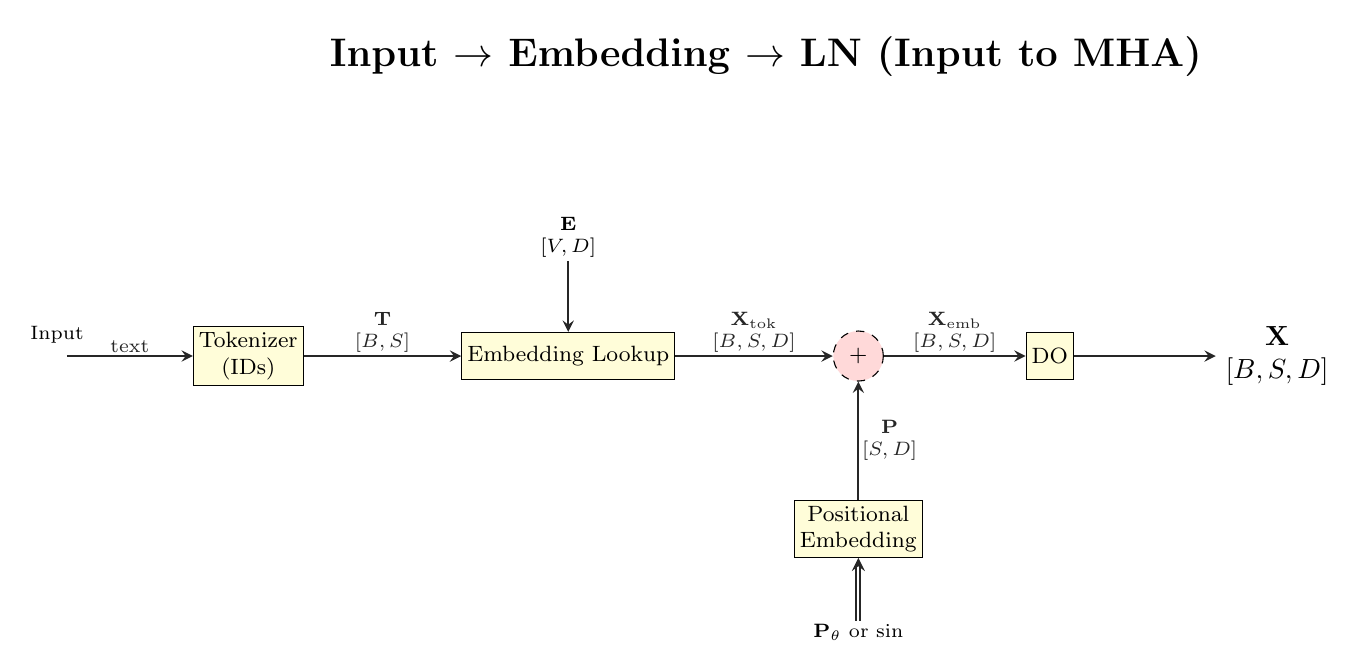
\begin{tikzpicture}[
  >=stealth,
  auxnode/.style={draw, rectangle, fill=yellow!15, minimum height=6mm, inner sep=2pt, font=\footnotesize, align=center},
  mulnode/.style={draw, circle, fill=green!15, minimum size=6mm, font=\footnotesize, align=center},
  addnode/.style={draw, circle, dashed, fill=red!15, minimum size=6mm, font=\footnotesize, align=center},
  flow/.style={->, thick, black!85},
  flow2/.style={->, double, thick, black!85},
  dimlabel/.style={font=\scriptsize, inner sep=1pt, align=center}
]

\node[font=\Large\bfseries] at (9, 3.8) {Input $\rightarrow$ Embedding $\rightarrow$ LN (Input to MHA)};

% nodes
\node (RawText) at (0,0) {};
\node[auxnode, align=center] (Tok)   [right=1.6cm of RawText] {Tokenizer\\(IDs)};
\node[auxnode, align=center] (Lookup)[right=2.0cm of Tok]     {Embedding Lookup};
\node[addnode, minimum size=6mm] (Sum) [right=2.0cm of Lookup] {+};
\node[auxnode, align=center] (PosE)  [below=1.5cm of Sum]  {Positional\\Embedding};
\node[auxnode] (Drop) [right=1.8cm of Sum] {DO};
\node (OUTPUT)   [align=center, right=1.8cm of Drop]   {$\mathbf{X}$\\$[B,S,D]$};

% parameter/const “double” edges
\node[dimlabel] (Eparam) [align=center, above=0.9cm of Lookup] {$\mathbf{E}$\\$[V,D]$};
\node[dimlabel] (Pparam) [align=center, below=0.8cm of PosE]   {$\mathbf{P}_{\theta}$ or sin};

% flows
\draw[flow] (RawText) -- (Tok) node[dimlabel, midway, above]
  {$\text{text}$};
\draw[flow] (Tok) -- (Lookup) node[dimlabel, midway, above]
  {$\mathbf{T}$\\$[B,S]$};

% Embedding matrix E
\draw[flow] (Eparam) -- (Lookup);

% Lookup -> Sum (token embeddings)
\draw[flow] (Lookup) -- (Sum) node[dimlabel, midway, above]
  {$\mathbf{X}_{\text{tok}}$\\$[B,S,D]$};

% Positional embedding path
\draw[flow] (PosE) -- (Sum) node[dimlabel, midway, right]
  {$\mathbf{P}$\\$[S,D]$};

% Optional: show P as parameter (sinusoidal/learned)
\draw[flow2] (Pparam) -- (PosE) ;

\draw[flow] (Sum) -- (Drop) node[dimlabel, midway, above]
  {$\mathbf{X}_{\text{emb}}$\\$[B,S,D]$};
\draw[flow] (Drop) -- (OUTPUT);

% labels for start and destination
\node[dimlabel, above=0.0cm of RawText] {Input};

\end{tikzpicture}%
}

\newpage
\renewcommand{\arraystretch}{1.2}
\small

% -------- Operations (Ops) --------
\begin{center}
\textbf{Operations (Ops)}
\begin{tabular}{llll}
\hline
\textbf{Abbrev} & \textbf{Name} & \textbf{Type / Shape} & \textbf{Notes} \\
\hline
Tokenizer & Tokenizer (IDs) & op & Maps raw text $\to$ integer ids $\mathbf{T}\in\mathbb{Z}^{[B,S]}$. \\
Embedding Lookup & Embedding Lookup & op & Gathers rows from $\mathbf{E}\in\mathbb{R}^{V\times D}$ using ids $\mathbf{T}$. \\
$+$ & Element-wise Add (dashed circle) & op & Adds token and positional embeddings; broadcasting over $B,S$ if needed. \\
DO & Dropout & op & Training-time stochastic dropout on $\mathbf{X}_{\text{emb}}$; identity at inference. \\
\textit{(none)} & Broadcast $\mathrm{BC}_{B,S}(\cdot)$ & op & Expands $[S,D]$ (or $[D]$) to $[B,S,D]$ across batch/sequence. \\
\hline
\end{tabular}
\end{center}

\vspace{0.8em}

% -------- Data Tensors (Values) --------
\begin{center}
\textbf{Data Tensors (Values)}
\begin{tabular}{llll}
\hline
\textbf{Symbol} & \textbf{Name} & \textbf{Shape} & \textbf{Notes} \\
\hline
text & Raw input text & — & Character/byte stream before tokenization. \\
$\mathbf{T}$ & Token ids & $[B,S]$ & Output of Tokenizer; integers in $\{0,\dots,V{-}1\}$. \\
$\mathbf{E}$ & Embedding matrix (params) & $[V,D]$ & Trainable; each vocab entry has a $D$-dim vector. \\
$\mathbf{X}_{\text{tok}}$ & Token embeddings & $[B,S,D]$ & $\mathrm{lookup}(\mathbf{E}, \mathbf{T})$. \\
$\mathbf{P}$ & Positional embedding & $[S,D]$ (or $[B,S,D]$) & Learned $\mathbf{P}_\theta$ \textbf{or} sinusoidal (fixed); broadcast to $[B,S,D]$. \\
$\mathbf{X}_{\text{emb}}$ & Sum of token+pos & $[B,S,D]$ & $\mathbf{X}_{\text{tok}} + \mathrm{BC}_{B,S}(\mathbf{P})$. \\
$\mathbf{X}$ & Input to MHA & $[B,S,D]$ & After dropout (DO); goes to LN/MHA stack. \\
$\mathbf{P}_\theta$ & Learned pos. params & matches $\mathbf{P}$ & Used when positions are trainable; otherwise “sin” denotes fixed sinusoidal. \\
\hline
\multicolumn{4}{l}{\textbf{Shape symbols:}\; $B$=batch size,\; $S$=sequence length,\; $D$=model dim,\; $V$=vocab size.} \\
\multicolumn{4}{l}{\textbf{Notes:}\; In practice, $\mathbf{P}$ may be pre-broadcast to $[B,S,D]$ or added per-token with implicit broadcasting.} \\
\hline
\end{tabular}
\end{center}

\end{document}

  \caption{Input embedding forward pass. Token IDs are mapped to token
  embeddings using $\mathbf{E}$, positional embeddings $\mathbf{P}$ are
  added, and optional dropout yields the initial hidden states
  $\mathbf{X} \in [B,S,D]$.}
  \label{fig:single_node_input_embedding}
\end{figure}

In the backward pass (not shown as a separate figure), gradients with
respect to the embeddings are accumulated into the token embedding
matrix $\mathbf{E}$ and positional table $\mathbf{P}$ by summing over all
positions where each embedding is used.


% ------------------------ 5.2 Multi-Head Attention -------------------
\subsection{Multi-Head Attention (MHA)}

Multi-Head Attention enables the model to jointly attend to information
from different representation subspaces. The mechanism involves:

\begin{itemize}
  \item \textbf{Linear projections}: mapping inputs to queries (Q),
        keys (K), and values (V).
  \item \textbf{Scaled dot-product attention}: computing attention scores
        and weighted sums of values.
  \item \textbf{Multi-head splitting}: processing $N_H$ attention heads
        in parallel, each with dimension $D_h$ such that $D = N_H D_h$.
  \item \textbf{Output projection}: concatenating heads and projecting
        back to the model dimension.
\end{itemize}

Given input activations $\mathbf{X} \in [B,S,D]$, the forward pass uses
layer normalization, QKV projections, attention over the sequence, and a
residual connection back to $\mathbf{X}$. The overall structure of this
computation is visualized in
Figure~\ref{fig:single_node_mha_forward}, while the corresponding gradient
flow during training is shown in
Figure~\ref{fig:single_node_mha_backward}.

\subsubsection{Forward Pass}

Given input activations $\mathbf{X} \in \mathbb{R}^{B \times S \times D}$,
the multi-head self-attention block computes an output
$\mathbf{A}_{\text{out}} \in \mathbb{R}^{B \times S \times D}$ that will be
fed into the following MLP block. The same tensor shapes and operations
are annotated along the edges of
Figure~\ref{fig:single_node_mha_forward} for quick visual reference.

\paragraph{(1) Layer normalization on the input.}
We first normalize the input along the hidden dimension:
\[
  \mathbf{X}_{\text{norm}} = \mathrm{LN}(\mathbf{X}) \in \mathbb{R}^{B \times S \times D}.
\]
Layer normalization is parameterized by learnable scale and bias vectors
$\boldsymbol{\gamma}, \boldsymbol{\beta} \in \mathbb{R}^{D}$, but for
brevity we only track the normalized activations here. In
Figure~\ref{fig:single_node_mha_forward}, this corresponds to the leftmost
normalization block before the Q/K/V projections.

\paragraph{(2) Linear projections to Q, K, V.}
From $\mathbf{X}_{\text{norm}}$ we compute queries, keys, and values via
three independent linear layers:
\[
  \mathbf{Q} = \mathbf{X}_{\text{norm}} W_Q,\quad
  \mathbf{K} = \mathbf{X}_{\text{norm}} W_K,\quad
  \mathbf{V} = \mathbf{X}_{\text{norm}} W_V,
\]
where $W_Q, W_K, W_V \in \mathbb{R}^{D \times D}$. Each of these tensors
is then reshaped into a head-major representation,
\[
  \mathbf{Q},\mathbf{K},\mathbf{V}
    \;\in\; \mathbb{R}^{B \times N_H \times S \times D_h},
  \qquad D = N_H \cdot D_h.
\]
These projections and reshapes are drawn explicitly in the upper left of
Figure~\ref{fig:single_node_mha_forward}, where each head receives its own
$D_h$-dimensional slice.

\paragraph{(3) Scaled dot-product attention per head.}
For each head, we form attention scores by a scaled dot-product between
queries and keys:
\[
  \mathbf{S} = \frac{\mathbf{Q}\mathbf{K}^{\top}}{\sqrt{D_h}}
  \;\in\; \mathbb{R}^{B \times N_H \times S \times S},
\]
where the last two dimensions correspond to
(query position, key position). A causal mask or padding mask is applied
to $\mathbf{S}$ to prevent attending to invalid positions. After masking,
a softmax along the last dimension produces attention weights:
\[
  \mathbf{A}_{S} = \mathrm{Softmax}(\mathrm{Mask}(\mathbf{S}))
  \;\in\; \mathbb{R}^{B \times N_H \times S \times S}.
\]
These weights are then used to aggregate values:
\[
  \mathbf{A}_{\text{heads}} = \mathbf{A}_{S}\mathbf{V}
  \;\in\; \mathbb{R}^{B \times N_H \times S \times D_h},
\]
as depicted in the central part of
Figure~\ref{fig:single_node_mha_forward}, where each head computes a
weighted sum over the value vectors.

\paragraph{(4) Head concatenation and output projection.}
The per-head outputs are concatenated along the head dimension and
reshaped back to the model dimension:
\[
  \mathbf{A}_{\text{cat}}
    = \mathrm{ConcatHeads}(\mathbf{A}_{\text{heads}})
    \;\in\; \mathbb{R}^{B \times S \times D}.
\]
A final output projection maps this back into the same hidden space:
\[
  \mathbf{A}_{\text{lin}} = \mathbf{A}_{\text{cat}} W_O + \mathbf{b}_O,
  \qquad W_O \in \mathbb{R}^{D \times D},\;
         \mathbf{b}_O \in \mathbb{R}^{D}.
\]
This corresponds to the right side of
Figure~\ref{fig:single_node_mha_forward}, where all heads are merged and
projected back to $[B,S,D]$.

\paragraph{(5) Dropout and residual connection.}
During training, dropout may be applied to $\mathbf{A}_{\text{lin}}$:
\[
  \mathbf{A}_{\text{drop}} = \mathrm{Dropout}(\mathbf{A}_{\text{lin}}),
\]
and the result is added back to the original input via a residual
connection:
\[
  \mathbf{A}_{\text{out}} = \mathbf{X} + \mathbf{A}_{\text{drop}}
  \;\in\; \mathbb{R}^{B \times S \times D}.
\]
The final sum node and residual edge are explicitly shown on the far right
of Figure~\ref{fig:single_node_mha_forward}. This
$\mathbf{A}_{\text{out}}$ becomes the input to the subsequent MLP block.

\begin{landscape}
\begin{figure}[p]
  \centering
  \resizebox{\linewidth}{!}{%
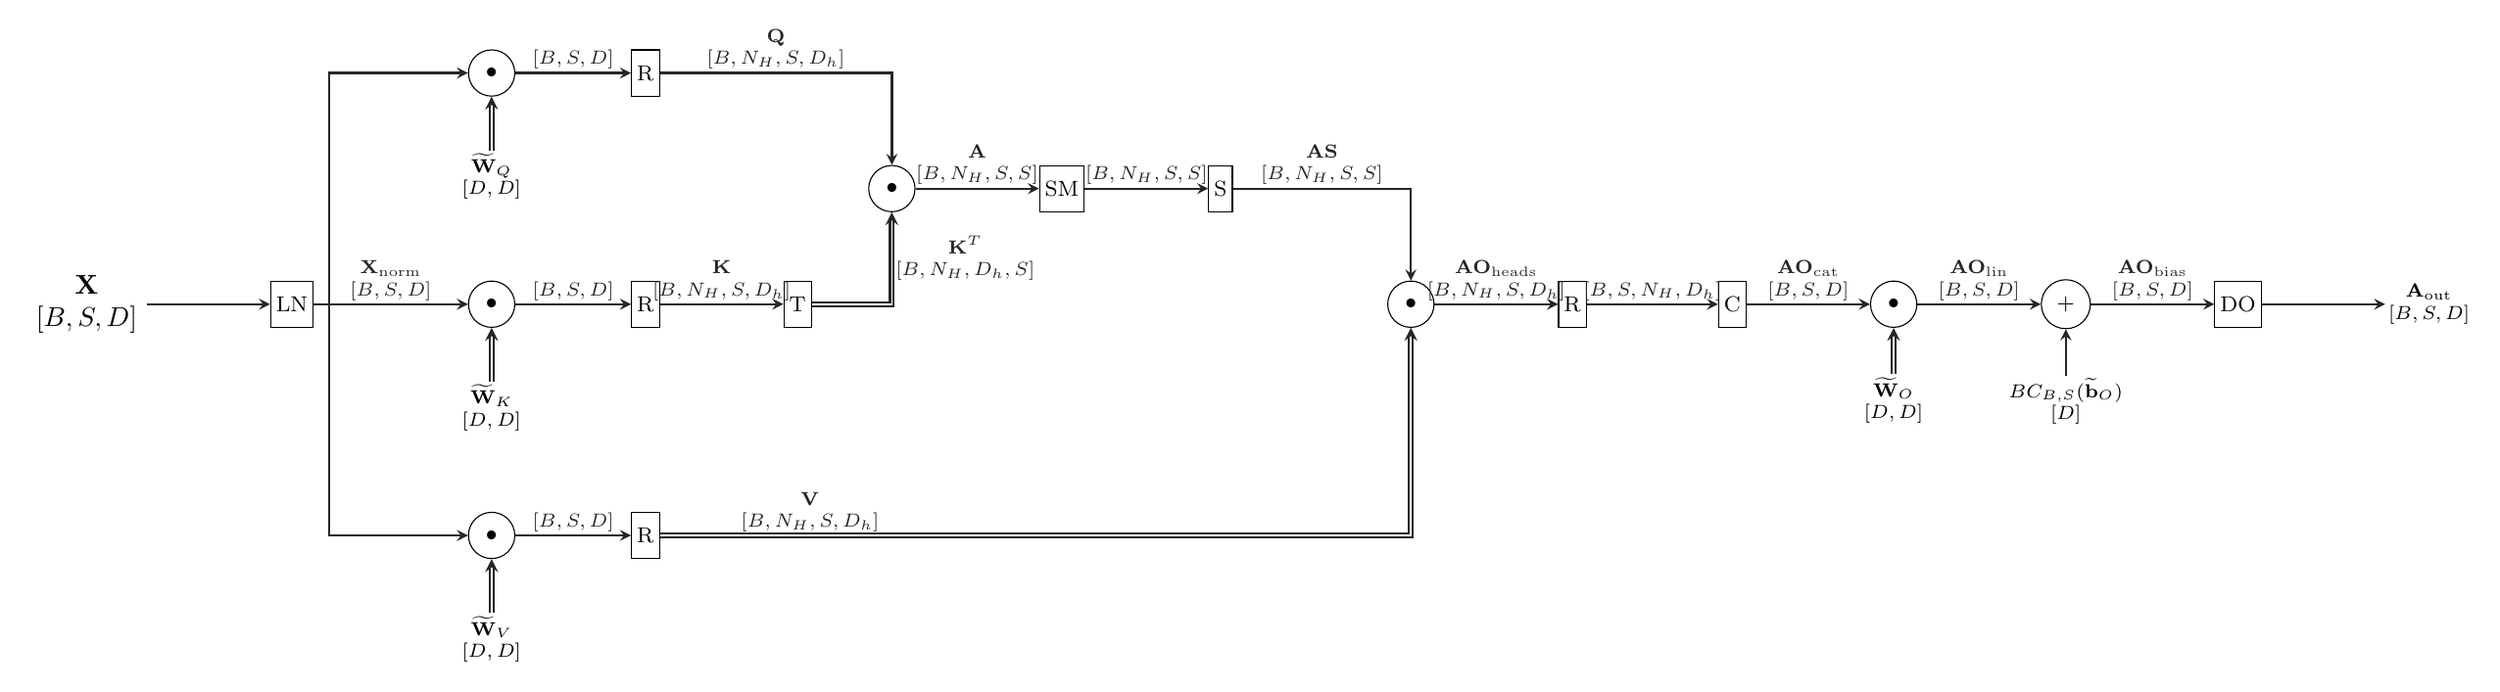
\begin{tikzpicture}[
  every node/.style={transform shape},
  >=stealth,
  auxnode/.style={draw, rectangle, fill=white, minimum height=6mm, inner sep=2pt, font=\footnotesize, align=center},
  mulnode/.style={draw, circle, fill=white, minimum size=6mm, font=\footnotesize, align=center},
  addnode/.style={draw, circle, fill=white, minimum size=6mm, font=\footnotesize, align=center},
  flow/.style={->, thick, black!85},
  flow2/.style={->, double, thick, black!85},
  dimlabel/.style={font=\scriptsize, inner sep=1pt, align=center}
]
% \node[font=\Large\bfseries] at (8, 4.5) {Multi-Head Attention Forward Pass};

\node (Input) at (0.5, 0) [align=center] {$\mathbf{X}$\\$[B,S,D]$};
\node[auxnode] (LN) [right=1.6cm of Input] {LN};

\node[mulnode] (Proj_Q) [right=2.0cm of LN, yshift=3.0cm] {$\bullet$};
\node[auxnode] (R_Q) [right=1.5cm of Proj_Q] {R};

\node[mulnode] (Proj_K) [right=2.0cm of LN, yshift=0cm] {$\bullet$};
\node[auxnode] (R_K) [right=1.5cm of Proj_K] {R};

\node[mulnode] (Proj_V) [right=2.0cm of LN, yshift=-3.0cm] {$\bullet$};
\node[auxnode] (R_V) [right=1.5cm of Proj_V] {R};

\node[dimlabel] (WQ) [align=center, below=0.7cm of Proj_Q] {$\widetilde{\mathbf{W}}_{Q}$\\$[D,D]$};
\node[dimlabel] (WK) [align=center, below=0.7cm of Proj_K] {$\widetilde{\mathbf{W}}_{K}$\\$[D,D]$};
\node[dimlabel] (WV) [align=center, below=0.7cm of Proj_V] {$\widetilde{\mathbf{W}}_{V}$\\$[D,D]$};

\node[auxnode] (T_K) [right=1.6cm of R_K] {T};
\node[mulnode] (QK) [right=2.7cm of R_Q, yshift=-1.5cm] {$\bullet$};
\node[auxnode] (SM) [right=1.6cm of QK] {SM};
\node[auxnode] (Soft) [right=1.6cm of SM] {S};
\node[mulnode] (PV) [right=2.0cm of Soft, yshift=-1.5cm] {$\bullet$};

\node[auxnode] (R_Merge) [right=1.6cm of PV] {R};
\node[auxnode] (Cat) [right=1.7cm of R_Merge] {C};

\node[mulnode] (OProj) [right=1.6cm of Cat] {$\bullet$};
\node[dimlabel] (WO_FWD) [align=center, below=0.6cm of OProj] {$\widetilde{\mathbf{W}}_{O}$\\$[D,D]$};
\node[addnode] (AddB) [right=1.6cm of OProj] {+};
\node[dimlabel] (BO) [align=center, below=0.6cm of AddB] {$BC_{B,S}(\widetilde{\mathbf{b}}_{O})$\\$[D]$};
\node[auxnode] (Drop) [right=1.6cm of AddB] {DO};
\node[dimlabel] (Aout) [align=center, right=1.6cm of Drop] {$\mathbf{A}_{\text{out}}$\\$[B,S,D]$};

\draw[flow] (Input) -- (LN);

\draw[flow] (LN.east) -- ++(0.2,0) |- (Proj_Q.west);
\draw[flow] (LN) -- (Proj_K.west) node[dimlabel, midway, above]{$\mathbf{X}_{\text{norm}}$\\$[B,S,D]$};
\draw[flow] (LN.east) -- ++(0.2,0) |- (Proj_V.west);

\draw[flow2] (WQ) -- (Proj_Q);
\draw[flow2] (WK) -- (Proj_K);
\draw[flow2] (WV) -- (Proj_V);

\draw[flow] (Proj_Q) -- (R_Q) node[dimlabel, midway, above]{$[B,S,D]$};
\draw[flow] (Proj_K) -- (R_K) node[dimlabel, midway, above]{$[B,S,D]$};
\draw[flow] (Proj_V) -- (R_V) node[dimlabel, midway, above]{$[B,S,D]$};

\draw[flow] (R_Q) -| (QK) node[dimlabel, near start, above]{$\mathbf{Q}$\\$[B,N_H,S,D_h]$};
\draw[flow] (R_K) -- (T_K) node[dimlabel, midway, above]{$\mathbf{K}$\\$[B,N_H,S,D_h]$};
\draw[flow2] (T_K) -| (QK) node[dimlabel, near end, right]{$\mathbf{K}^{T}$\\$[B,N_H,D_h,S]$};

\draw[flow] (QK) -- (SM) node[dimlabel, midway, above]{$\mathbf{A}$\\$[B,N_H,S,S]$};
\draw[flow] (SM) -- (Soft) node[dimlabel, midway, above]{$[B,N_H,S,S]$};
\draw[flow] (Soft) -| (PV) node[dimlabel, near start, above]{$\mathbf{AS}$\\$[B,N_H,S,S]$};
\draw[flow2] (R_V) -| (PV) node[dimlabel, pos=0.1, above]{$\mathbf{V}$\\$[B,N_H,S,D_h]$};

\draw[flow] (PV) -- (R_Merge) node[dimlabel, midway, above]{$\mathbf{AO}_{\text{heads}}$\\$[B,N_H,S,D_h]$};
\draw[flow] (R_Merge) -- (Cat) node[dimlabel, midway, above]{$[B,S,N_H,D_h]$};
\draw[flow] (Cat) -- (OProj) node[dimlabel, midway, above]{$\mathbf{AO}_{\text{cat}}$\\$[B,S,D]$};
\draw[flow2] (WO_FWD) -- (OProj);
\draw[flow] (OProj) -- (AddB) node[dimlabel, midway, above]{$\mathbf{AO}_{\text{lin}}$\\$[B,S,D]$};
\draw[flow] (BO) -- (AddB);
\draw[flow] (AddB) -- (Drop) node[dimlabel, midway, above]{$\mathbf{AO}_{\text{bias}}$\\$[B,S,D]$};
\draw[flow] (Drop) -- (Aout);
\end{tikzpicture}%
}

  \caption{Multi-head attention forward pass on a single node.
  Input activations $\mathbf{X}$ are layer-normalized, projected to
  $\mathbf{Q}$, $\mathbf{K}$, and $\mathbf{V}$, processed by scaled
  dot-product attention over the sequence, concatenated across heads, and
  projected back to $[B,S,D]$ with an output projection and residual
  connection.}
  \label{fig:single_node_mha_forward}
\end{figure}
\end{landscape}

\subsubsection{Backward Pass}

In the backward pass, gradients arrive from the residual output and
propagate through the output projection, attention mechanism, QKV
projections, and layer normalization. Figure~\ref{fig:single_node_mha_backward}
mirrors Figure~\ref{fig:single_node_mha_forward} but with dashed arrows
showing gradient flow and explicit nodes for each matrix multiplication in
the backward path.

At a high level:

\begin{itemize}
  \item Gradients from the loss provide $\mathrm{d}\mathbf{A}_{\text{out}}$
        at the output of the attention block, which are split between the
        residual branch and the main path, as shown on the right of
        Figure~\ref{fig:single_node_mha_backward}.
  \item The output projection is backpropagated to obtain gradients for
        weights and biases and to recover $\mathrm{d}\mathbf{A}_{\text{cat}}$
        before head concatenation.
  \item The per-head attention computation is differentiated to obtain
        $\mathrm{d}\mathbf{V}$ and $\mathrm{d}\mathbf{A}_{S}$, and then
        $\mathrm{d}\mathbf{Q}$ and $\mathrm{d}\mathbf{K}$ through the
        scaled dot-product and softmax, corresponding to the central
        region of Figure~\ref{fig:single_node_mha_backward}.
  \item QKV projection layers accumulate gradients for
        $\mathbf{W}_Q, \mathbf{W}_K, \mathbf{W}_V$ and produce
        $\mathrm{d}\mathbf{X}_{\text{norm}}$, shown on the left side of
        Figure~\ref{fig:single_node_mha_backward}.
  \item Layer normalization backward finally produces
        $\mathrm{d}\mathbf{X}$ that flows to the previous block and
        parameter gradients for the LN parameters.
\end{itemize}

\begin{landscape}
\begin{figure}[p]
  \resizebox{\linewidth}{!}{%
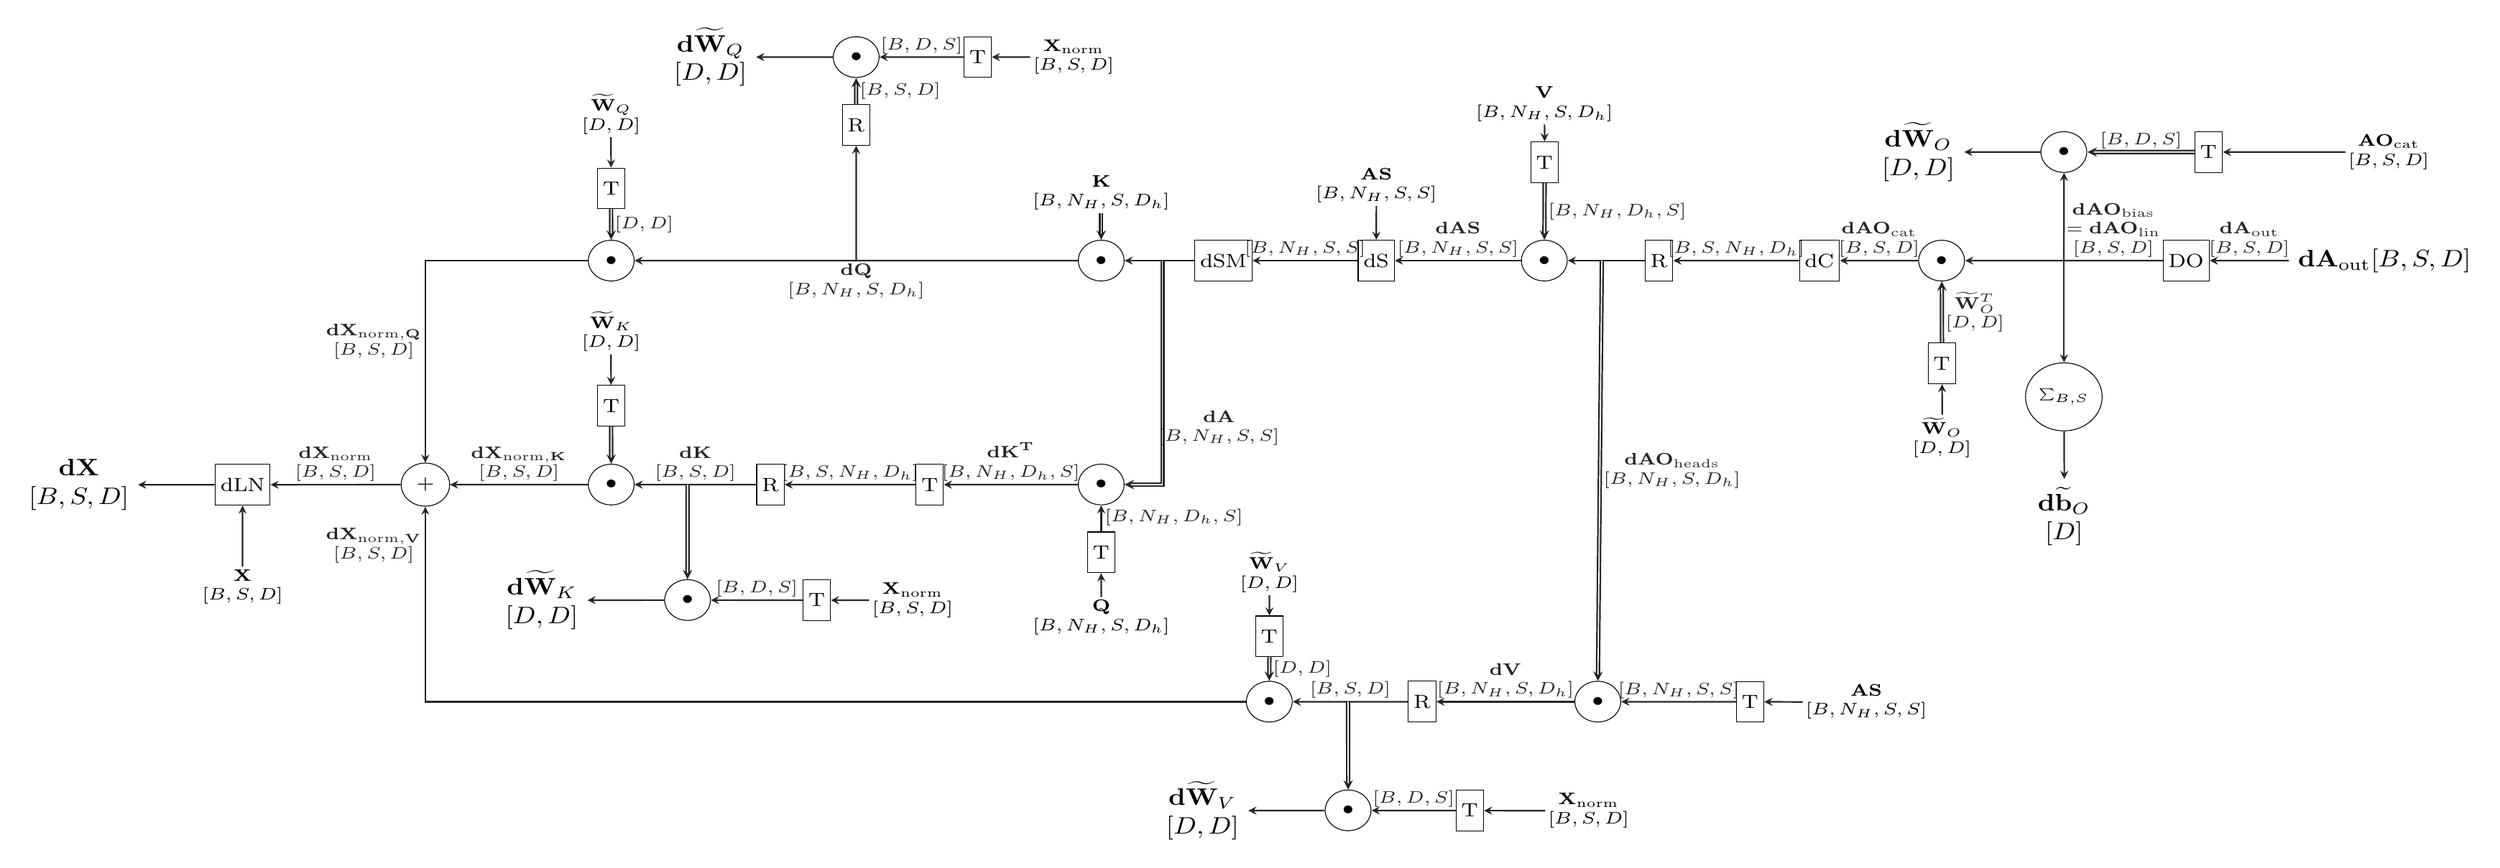
\begin{tikzpicture}[
  every node/.style={transform shape},
  >=stealth,
  auxnode/.style={draw, rectangle, fill=white, minimum height=6mm, inner sep=2pt, font=\footnotesize, align=center},
  mulnode/.style={draw, circle, fill=white, minimum size=6mm, font=\footnotesize, align=center},
  addnode/.style={draw, circle, fill=white, minimum size=6mm, font=\footnotesize, align=center},
  sumnode/.style={draw, circle, fill=white, minimum size=6mm, font=\tiny, align=center},
  flow/.style={->, thick, black!85},
  flow2/.style={->, double, thick, black!85},
  dimlabel/.style={font=\scriptsize, inner sep=1pt, align=center},
  gradflow/.style={->, thick, black!85},
  gradweight/.style={->, thick, black!85}
]

\begin{scope}[xscale=1.35, yscale=1.2]

\def\yoffset{-1.0}
\def\dVXyoffset{-6.5}

\coordinate (Grad_Aout_B) at (17.5, \yoffset);
\coordinate (dDrop_center) at (15.9, \yoffset);
\coordinate (ProjGradSplit) at (14.3, \yoffset);
\coordinate (dOProj_center) at (12.7, \yoffset);
\coordinate (C_center) at (11.1, \yoffset);
\coordinate (R_center) at (9.0, \yoffset);
\coordinate (dPV_AS_calc_center) at (7.5, \yoffset);
\coordinate (dSoft_center) at (5.3, \yoffset);
\coordinate (dSM_calc_center) at (3.3, \yoffset);
\coordinate (dV_calc_center) at (8.2, \dVXyoffset+\yoffset);
\coordinate (R_V_bwd_center) at (5.9, \dVXyoffset+\yoffset);
\coordinate (dVX_calc_center) at (3.9, \dVXyoffset+\yoffset);
\coordinate (dQK_calc_Q_center) at (1.7, \yoffset);
\coordinate (dQK_calc_K_center) at (1.7, -3.3+\yoffset);
\coordinate (K_BWD_input_center) at (1.7, 1.0+\yoffset);
\coordinate (T_Q_bwd_center) at (1.7, -4.3+\yoffset);

% \node[font=\Large\bfseries] at (8, 4.6+\yoffset) {Multi-Head Attention Backward Pass};

\node (Grad_Aout_B) at (18.5, \yoffset) {$\mathbf{dA}_{\text{out}}$\\$[B,S,D]$};
\node[auxnode] (DO) at (dDrop_center) {DO};
\node[mulnode] (dOProj) at (dOProj_center) {$\bullet$};

\node[auxnode] (T_WO) [below=0.9cm of dOProj] {T};
\node[dimlabel] (WO_BWD) [below=0.45cm of T_WO] {$\widetilde{\mathbf{W}}_{O}$\\$[D,D]$};

\node[mulnode] (dWO_calc) at ($(ProjGradSplit)+(0, 1.6)$) {$\bullet$};
\node[align=center, left=1.0cm of dWO_calc]
  (dWO_GRAD) {$\mathbf{d}\widetilde{\mathbf{W}}_{O}$\\$[D,D]$};
\node[auxnode] (T_AO_in) [right=1.4cm of dWO_calc] {T};
\node[dimlabel] (AO_in_local_label) [right=1.6cm of T_AO_in] {$\mathbf{AO}_{\text{cat}}$\\$[B,S,D]$};

\node[auxnode] (C) at (C_center) {dC};
\node[auxnode] (R) at (R_center) {R};

\node[mulnode] (dPV_AS_calc) at (dPV_AS_calc_center) {$\bullet$};
\node[auxnode] (dSoft) at (dSoft_center) {dS};
\node[auxnode] (dSM_calc) at (dSM_calc_center) {dSM};

\node[mulnode] (dQK_calc_Q) at (dQK_calc_Q_center) {$\bullet$};
\node[mulnode] (dQX_proj_calc) [left=5.8cm of dQK_calc_Q] {$\bullet$};

\node[mulnode] (dQK_calc_K) at (dQK_calc_K_center) {$\bullet$};
\node[mulnode] (dKX_proj_calc) [left=5.8cm of dQK_calc_K] {$\bullet$};

\node[dimlabel] (K_BWD_input) at (K_BWD_input_center) {$\mathbf{K}$\\$[B,N_H,S,D_h]$};
\node[auxnode] (T_Q_bwd) at (T_Q_bwd_center) {T};
\node[dimlabel] (Q_BWD_input) [below=0.35cm of T_Q_bwd] {$\mathbf{Q}$\\$[B,N_H,S,D_h]$};

\node[dimlabel] (V_FWD) [above=1.7cm of dPV_AS_calc] {$\mathbf{V}$\\$[B,N_H,S,D_h]$};
\node[auxnode] (T_V_bwd) [below=0.25cm of V_FWD] {T};

\node[mulnode] (dV_calc) at (dV_calc_center) {$\bullet$};
\node[auxnode] (T_AS_bwd) [right=1.5cm of dV_calc] {T};
\node[dimlabel] (AS_BWD_for_V) [right=0.5cm of T_AS_bwd] {$\mathbf{AS}$\\$[B,N_H,S,S]$};

\node[auxnode] (R_V_bwd) at (R_V_bwd_center) {R};
\node[mulnode] (dVX_calc) at (dVX_calc_center) {$\bullet$};

\node[auxnode] (T_WV) [above=0.35cm of dVX_calc] {T};
\node[dimlabel] (WV_BWD) [above=0.3cm of T_WV] {$\widetilde{\mathbf{W}}_{V}$\\$[D,D]$};

\node[sumnode] (Sum_dBO) [below=1.5cm of ProjGradSplit] {$\sum_{B, S}$};
\node (dBO) [align=center, below=0.7cm of Sum_dBO] {$\mathbf{d}\widetilde{\mathbf{b}}_{O}$\\$[D]$};

\draw[gradflow] (Grad_Aout_B) -- (DO)
  node[dimlabel, midway, above]{$\mathbf{dA}_{\text{out}}$\\$[B,S,D]$};

\draw[gradflow] (DO) -- (dOProj)
  node[dimlabel, pos=0.25, above]{$\mathbf{dAO}_{\text{bias}}$\\$=\mathbf{dAO}_{\text{lin}}$\\$[B,S,D]$};

\draw[gradflow] (ProjGradSplit) -- (dWO_calc.south);
\draw[gradflow] (ProjGradSplit) -- ([yshift=-0.75cm]ProjGradSplit) -| (Sum_dBO.north);

\draw[gradflow] (dOProj) -- (C)
  node[dimlabel, midway, above]{$\mathbf{dAO}_{\text{cat}}$\\$[B,S,D]$};
\draw[gradflow] (C) -- (R)
  node[dimlabel, midway, above]{$[B,S,N_H,D_h]$};

\coordinate (R_split_point) at ($(dPV_AS_calc)!0.5!(R)$);
\draw[gradflow] (R.west) -- (dPV_AS_calc.east);
\draw[flow2] (R_split_point) -- (dV_calc.north)
  node[dimlabel, midway, right]{$\mathbf{dAO}_{\text{heads}}$\\$[B,N_H,S,D_h]$};

\draw[gradflow] (V_FWD.south) -- (T_V_bwd.north);
\draw[flow2] (T_V_bwd.south) -- (dPV_AS_calc.north)
  node[dimlabel, midway, right]{$[B,N_H,D_h,S]$};
\draw[gradflow] (dPV_AS_calc.west) -- (dSoft.east)
  node[dimlabel, midway, above]{$\mathbf{dAS}$\\$[B,N_H,S,S]$};

\node (AS_BWD_dS) [dimlabel, above=0.5cm of dSoft] {$\mathbf{AS}$\\$[B,N_H,S,S]$};
\draw[gradflow] (AS_BWD_dS.south) -- (dSoft.north);
\draw[gradflow] (dSoft.west) -- (dSM_calc.east)
  node[dimlabel, midway, above]{$[B,N_H,S,S]$};

\coordinate (dA_Split_X) at ($(dSM_calc_center)!0.5!(dQK_calc_Q_center)$);
\coordinate (dA_Split) at (dA_Split_X |- dQK_calc_Q.east);
\draw[gradflow] (dSM_calc.west) -- (dQK_calc_Q.east);
\draw[flow2] (dA_Split) -- (dA_Split |- dQK_calc_K.east) -- (dQK_calc_K.east)
  node[dimlabel, pos=-1.5, above, yshift=15]{$\mathbf{dA}$\\$[B,N_H,S,S]$};

\draw[flow2] (K_BWD_input.south) -- (dQK_calc_Q.north);
\draw[gradweight] (dQK_calc_Q) -- (dQX_proj_calc)
  node[dimlabel, midway, below]{$\mathbf{dQ}$\\$[B,N_H,S,D_h]$};

\node[auxnode] (T_WQ_bwd) [above=0.45cm of dQX_proj_calc] {T};
\node[dimlabel] (WQ_bwd) [above=0.45cm of T_WQ_bwd] {$\widetilde{\mathbf{W}}_{Q}$\\$[D,D]$};
\draw[flow] (WQ_bwd) -- (T_WQ_bwd);
\draw[flow2] (T_WQ_bwd.south) -- (dQX_proj_calc.north)
  node[dimlabel, midway, right]{$[D,D]$};

\draw[flow] (Q_BWD_input.north) -- (T_Q_bwd.south);
\draw[flow] (T_Q_bwd.north) -- (dQK_calc_K.south)
  node[dimlabel, pos=0.55, right]{$[B,N_H,D_h,S]$};

\node[auxnode] (T_dK) at ($(dQK_calc_K)!0.35!(dKX_proj_calc)$) {T};
\node[auxnode] (R_dK_mid) at ($(T_dK)!0.5!(dKX_proj_calc)$) {R};

\draw[gradweight] (dQK_calc_K) -- (T_dK)
  node[dimlabel, midway, above]{$\mathbf{dK^T}$\\$[B,N_H,D_h,S]$};
\draw[gradweight] (T_dK) -- (R_dK_mid)
  node[dimlabel, midway, above]{$[B,S,N_H,D_h]$};
\draw[gradweight] (R_dK_mid) -- (dKX_proj_calc)
  node[dimlabel, midway, above]{$\mathbf{dK}$\\$[B,S,D]$};

\node[auxnode] (T_WK_bwd) [above=0.55cm of dKX_proj_calc] {T};
\node[dimlabel] (WK_bwd) [above=0.45cm of T_WK_bwd] {$\widetilde{\mathbf{W}}_{K}$\\$[D,D]$};
\draw[gradflow] (WK_bwd) -- (T_WK_bwd);
\draw[flow2] (T_WK_bwd.south) -- (dKX_proj_calc.north);

\draw[gradflow] (AS_BWD_for_V.west) -- (T_AS_bwd.east);
\draw[gradflow] (T_AS_bwd.west) -- (dV_calc.east)
  node[dimlabel, midway, above]{$[B,N_H,S,S]$};
\draw[gradflow] (dV_calc.west) -- (R_V_bwd.east)
  node[dimlabel, midway, above]{$\mathbf{dV}$\\$[B,N_H,S,D_h]$};
\draw[gradflow] (R_V_bwd) -- (dVX_calc.east)
  node[dimlabel, midway, above]{$[B,S,D]$};

\draw[gradflow] (WV_BWD) -- (T_WV);
\draw[flow2] (T_WV) -- (dVX_calc.north)
  node[dimlabel, midway, right]{$[D,D]$};

\node[addnode] (Sum_dXnorm) [left=1.8cm of dKX_proj_calc] {$+$};

\draw[gradweight] (dQX_proj_calc.west) -| node[dimlabel, pos=0.7, left]{$\mathbf{dX}_{\text{norm},\mathbf{Q}}$\\$[B,S,D]$} (Sum_dXnorm.north);
\draw[gradweight] (dKX_proj_calc.west) -- node[dimlabel, midway, above]{$\mathbf{dX}_{\text{norm},\mathbf{K}}$\\$[B,S,D]$} (Sum_dXnorm.east);
\draw[gradweight] (dVX_calc.west) -| node[dimlabel, pos=0.9, left]{$\mathbf{dX}_{\text{norm},\mathbf{V}}$\\$[B,S,D]$} (Sum_dXnorm.south);

\coordinate (dV_branch) at ($(R_V_bwd.west)!0.52!(dVX_calc.east)$);
\node[mulnode] (dWV_mul) at ($(dV_branch)+(0,-1.6cm)$) {$\bullet$};
\draw[flow2] (dV_branch) -- (dWV_mul.north);

\node[auxnode] (T_Xnorm) [right=1.1cm of dWV_mul] {T};
\node[dimlabel] (Xnorm_local) [right=0.8cm of T_Xnorm] {$\mathbf{X}_{\text{norm}}$\\$[B,S,D]$};
\draw[gradflow] (Xnorm_local) -- (T_Xnorm);
\draw[gradflow] (T_Xnorm.west) -- (dWV_mul.east)
  node[dimlabel, midway, above]{$[B,D,S]$};
\node (dWV_out) [align=center, left=1.0cm of dWV_mul] {$\mathbf{d}\widetilde{\mathbf{W}}_{V}$\\$[D,D]$};
\draw[gradweight] (dWV_mul.west) -- (dWV_out);

\coordinate (dQ_branch) at ($(dQK_calc_Q.east)!0.50!(dQX_proj_calc.west)$);
\node[mulnode] (dWQ_mul) at ($(dQ_branch)+(0,3.0cm)$) {$\bullet$};
\node[auxnode] (R_dQ_for_WQ) at ($(dWQ_mul)+(0,-1.0cm)$) {R};
\draw[gradflow]  (dQ_branch) -- (R_dQ_for_WQ.south);
\draw[flow2] (R_dQ_for_WQ.north) -- (dWQ_mul.south)
  node[dimlabel, midway, right]{$[B,S,D]$};

\node[auxnode] (T_XnormQ) [right=1.1cm of dWQ_mul] {T};
\node[dimlabel] (Xnorm_localQ) [right=0.5cm of T_XnormQ] {$\mathbf{X}_{\text{norm}}$\\$[B,S,D]$};
\draw[gradflow] (Xnorm_localQ) -- (T_XnormQ);
\draw[gradflow] (T_XnormQ.west) -- (dWQ_mul.east)
  node[dimlabel, midway, above]{$[B,D,S]$};
\node (dWQ_out) [align=center, left=1.0cm of dWQ_mul] {$\mathbf{d}\widetilde{\mathbf{W}}_{Q}$\\$[D,D]$};
\draw[gradweight] (dWQ_mul.west) -- (dWQ_out);

\coordinate (dK_branch) at ($(R_dK_mid)!0.52!(dKX_proj_calc)$);
\node[mulnode] (dWK_mul) at ($(dK_branch)+(0,-1.7cm)$) {$\bullet$};
\draw[flow2]  (dK_branch) -- (dWK_mul.north);

\node[auxnode] (T_XnormK) [right=1.2cm of dWK_mul] {T};
\node[dimlabel, right=0.5cm of T_XnormK] (Xnorm_localK) {$\mathbf{X}_{\text{norm}}$\\$[B,S,D]$};
\draw[gradflow] (Xnorm_localK) -- (T_XnormK);
\draw[gradflow] (T_XnormK.west) -- (dWK_mul.east)
  node[dimlabel, midway, above]{$[B,D,S]$};
\node (dWK_out) [align=center, left=1.0cm of dWK_mul] {$\mathbf{d}\widetilde{\mathbf{W}}_{K}$\\$[D,D]$};
\draw[gradweight] (dWK_mul.west) -- (dWK_out);

\draw[gradweight] (Sum_dBO) -- (dBO);

\draw[gradflow] (WO_BWD) -- (T_WO);
\draw[flow2] (T_WO) -- (dOProj)
  node[dimlabel, midway, right]{$\widetilde{\mathbf{W}}_{O}^{T}$\\$[D,D]$};
\draw[gradflow] (AO_in_local_label) -- (T_AO_in);
\draw[flow2] (T_AO_in) -- (dWO_calc.east)
  node[dimlabel, midway, above]{$[B,D,S]$};
\draw[gradweight] (dWO_calc) -- (dWO_GRAD);

\node[auxnode] (dLN) [left=1.7cm of Sum_dXnorm] {dLN};
\draw[gradweight] (Sum_dXnorm.west) -- node[dimlabel, midway, above]
  {$\mathbf{dX}_{\text{norm}}$\\$[B,S,D]$} (dLN.east);

\node (dX_OUT) [align=center, left=1.0cm of dLN] {$\mathbf{dX}$\\$[B,S,D]$};
\draw[gradweight] (dLN.west) -- (dX_OUT);

\node[dimlabel] (LNCache) [below=0.9cm of dLN] {$\mathbf{X}$\\$[B,S,D]$};
\draw[gradflow] (LNCache.north) -- (dLN.south);

\end{scope}
\end{tikzpicture}
}

  \caption{Multi-head attention backward pass. The diagram shows
  how gradients from $\mathrm{d}\mathbf{A}_{\text{out}}$ are propagated
  through the output projection, attention heads, QKV projection matrices,
  and layer normalization to yield $\mathrm{d}\mathbf{X}$ and all associated
  weight and bias gradients.}
  \label{fig:single_node_mha_backward}
\end{figure}
\end{landscape}


% ------------------------ 5.3 MLP / FFN Block ------------------------
\subsection{Feed-Forward Network (MLP / FFN)}

The feed-forward network (FFN) applies two linear transformations with a
non-linear activation in between, independently at each position in the
sequence. Starting from $\mathbf{X}' \in [B,S,D]$ (the output of MHA with
residual), the FFN performs:

\begin{itemize}
  \item \textbf{Up-projection}:
        $[B,S,D] \rightarrow [B,S,D_{\text{ff}}]$ (expanding the dimension).
  \item \textbf{Activation}: GELU or ReLU non-linearity applied elementwise.
  \item \textbf{Down-projection}:
        $[B,S,D_{\text{ff}}] \rightarrow [B,S,D]$ (projecting back).
  \item \textbf{Dropout and residual}: dropout on the FFN output followed
        by a residual connection back to $\mathbf{X}'$.
\end{itemize}

The forward structure of this block is illustrated in
Figure~\ref{fig:single_node_mlp_forward}, and the corresponding backward
matmuls are expanded in
Figure~\ref{fig:single_node_mlp_backward}.

\subsubsection{Forward Pass}

\begin{figure}[htbp]
  \centering
  \resizebox{\linewidth}{!}{%
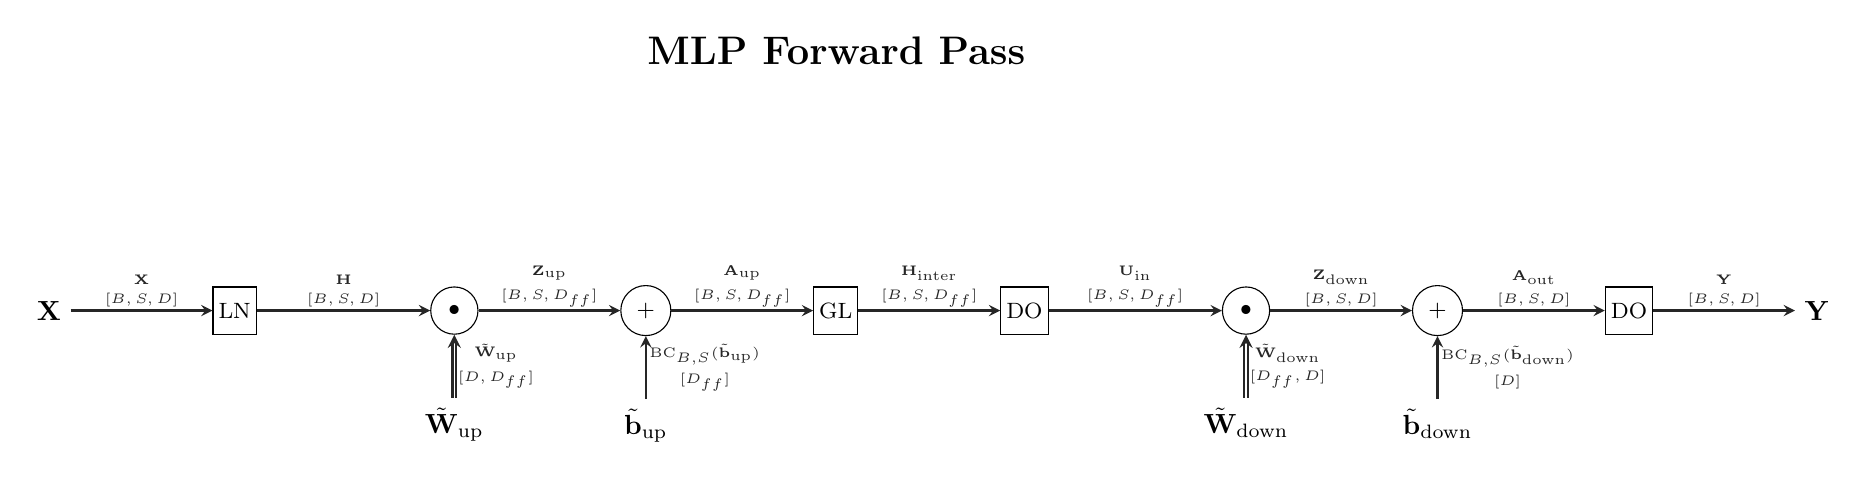
\begin{tikzpicture}[
    >=stealth,
    auxnode/.style={draw, rectangle, fill=white, minimum height=6mm, inner sep=2pt, font=\footnotesize, align=center},
    mulnode/.style={draw, circle, fill=white, minimum size=6mm, font=\footnotesize, align=center},
    addnode/.style={draw, circle, fill=white, minimum size=6mm, font=\footnotesize, align=center},
    sumnode/.style={draw, circle, fill=white, minimum size=6mm, font=\tiny, align=center},
    flow/.style={->, thick, black!85},
    flow2/.style={double, ->, thick, black!85},
    dimlabel/.style={font=\tiny, inner sep=1pt, align=center}
]
    \node[font=\Large\bfseries] at (10, 2.8) {MLP Forward Pass};

    \pgfmathsetmacro{\verticaloffset}{-0.5}

    \node            (MIn)   at (0,\verticaloffset) {$\mathbf{X}$};
    \node[auxnode]   (LN2)   [right=1.8cm of MIn] {LN};
    \node[mulnode]   (L1Mul) [right=2.2cm of LN2] {$\bullet$};
    \node            (Wup)   [below=0.8cm of L1Mul] {$\tilde{\mathbf{W}}_{\text{up}}$};
    \node[addnode]   (AddB1) [right=1.8cm of L1Mul] {+};
    \node            (Bup)   [below=0.8cm of AddB1] {$\tilde{\mathbf{b}}_{\text{up}}$};
    \node[auxnode]   (Act)   [right=1.8cm of AddB1] {GL};
    \node[auxnode]   (Drop1) [right=1.8cm of Act] {DO};
    \node[mulnode]   (L2Mul) [right=2.2cm of Drop1] {$\bullet$};
    \node            (Wdown) [below=0.8cm of L2Mul] {$\tilde{\mathbf{W}}_{\text{down}}$};
    \node[addnode]   (AddB2) [right=1.8cm of L2Mul] {+};
    \node            (Bdown) [below=0.8cm of AddB2] {$\tilde{\mathbf{b}}_{\text{down}}$};
    \node[auxnode]   (Drop2) [right=1.8cm of AddB2] {DO};
    \node            (MOut)  [right=1.8cm of Drop2] {$\mathbf{Y}$};

    \draw[flow] (MIn) -- (LN2) node[dimlabel, midway, above]{\shortstack{$\mathbf{X}$\\$[B,S,D]$}};
    \draw[flow] (LN2) -- (L1Mul) node[dimlabel, midway, above]{\shortstack{$\mathbf{H}$\\$[B,S,D]$}};
    \draw[flow2] (Wup) -- (L1Mul) node[dimlabel, midway, right]{\shortstack{$\tilde{\mathbf{W}}_{\text{up}}$\\$[D, D_{ff}]$}};
    \draw[flow] (L1Mul) -- (AddB1) node[dimlabel, midway, above]{\shortstack{$\mathbf{Z}_{\text{up}}$\\$[B,S,D_{ff}]$}};
    \draw[flow] (Bup) -- (AddB1) node[dimlabel, midway, right]{\shortstack{$\mathrm{BC}_{B,S}(\tilde{\mathbf{b}}_{\text{up}})$\\$[D_{ff}]$}};
    \draw[flow] (AddB1) -- (Act) node[dimlabel, midway, above]{\shortstack{$\mathbf{A}_{\text{up}}$\\$[B,S,D_{ff}]$}};
    \draw[flow] (Act) -- (Drop1) node[dimlabel, midway, above]{\shortstack{$\mathbf{H}_{\text{inter}}$\\$[B,S,D_{ff}]$}};
    \draw[flow] (Drop1) -- (L2Mul) node[dimlabel, midway, above]{\shortstack{$\mathbf{U}_{\text{in}}$\\$[B,S,D_{ff}]$}};
    \draw[flow2] (Wdown) -- (L2Mul) node[dimlabel, midway, right]{\shortstack{$\tilde{\mathbf{W}}_{\text{down}}$\\$[D_{ff}, D]$}};
    \draw[flow] (L2Mul) -- (AddB2) node[dimlabel, midway, above]{\shortstack{$\mathbf{Z}_{\text{down}}$\\$[B,S,D]$}};
    \draw[flow] (Bdown) -- (AddB2) node[dimlabel, midway, right]{\shortstack{$\mathrm{BC}_{B,S}(\tilde{\mathbf{b}}_{\text{down}})$\\$[D]$}};
    \draw[flow] (AddB2) -- (Drop2) node[dimlabel, midway, above]{\shortstack{$\mathbf{A}_{\text{out}}$\\$[B,S,D]$}};
    \draw[flow] (Drop2) -- (MOut) node[dimlabel, midway, above]{\shortstack{$\mathbf{Y}$\\$[B,S,D]$}};

\end{tikzpicture}%
}

  \caption{Feed-forward (MLP) forward pass. Hidden states are
  layer-normalized, projected up to dimension $D_{\text{ff}}$, passed
  through a non-linearity and dropout, projected back to $D$, and combined
  with the input via a residual connection.}
  \label{fig:single_node_mlp_forward}
\end{figure}

\subsubsection{Backward Pass}

The MLP backward pass is a canonical example of the ``2$\times$ cost''
rule: each forward matrix multiplication generates two backward matmuls
(one for activations, one for weights). Starting from
$\mathrm{d}\mathbf{Y}$ at the FFN output, the backward pass proceeds as:

\begin{enumerate}
  \item \textbf{Residual and dropout backward}: split $\mathrm{d}\mathbf{Y}$
        into the identity path and the path through the final dropout to
        obtain $\mathrm{d}\mathbf{Z}_{\text{down}}$.
  \item \textbf{Down-projection backward}: compute
        $\mathrm{d}\mathbf{U}$ (w.r.t.\ activations) and obtain
        gradients for $\mathbf{W}_{\text{down}}$ and
        $\mathbf{b}_{\text{down}}$.
  \item \textbf{Activation and dropout backward}: backpropagate through
        dropout and the non-linearity (e.g., GELU) to obtain
        $\mathrm{d}\mathbf{Z}_{\text{up}}$.
  \item \textbf{Up-projection backward}: compute
        $\mathrm{d}\mathbf{H}$ and gradients for
        $\mathbf{W}_{\text{up}}$ and $\mathbf{b}_{\text{up}}$.
  \item \textbf{Layer normalization backward}: propagate
        $\mathrm{d}\mathbf{H}$ through layer normalization to produce
        $\mathrm{d}\mathbf{X}'$ (which flows into the MHA block) and
        gradients for LN parameters.
\end{enumerate}

As with MHA, every matmul in the forward path corresponds to two matmuls
in the backward path, which are shown explicitly in
Figure~\ref{fig:single_node_mlp_backward}.

\begin{figure}[htbp]
  \centering
  \noindent
\resizebox{\linewidth}{!}{%
\begin{tikzpicture}[
    >=stealth,
    auxnode/.style={draw, rectangle, fill=white, minimum height=6mm, inner sep=2pt, font=\footnotesize, align=center},
    mulnode/.style={draw, circle, fill=white, minimum size=6mm, font=\footnotesize, align=center},
    addnode/.style={draw, circle, fill=white, minimum size=6mm, font=\footnotesize, align=center},
    sumnode/.style={draw, circle, fill=white, minimum size=6mm, font=\tiny, align=center},
    flow_rev/.style={<-, thick, black!85},
    flow_dw/.style={->, thick, black!85},
    flow_act/.style={double, ->, thick, black!85},
    dimlabel/.style={font=\tiny, inner sep=1pt, align=center},
    gradlabel/.style={font=\tiny\bfseries, inner sep=1pt, align=center}
]
    \node[font=\Large\bfseries] at (5, 10) {MLP Backward Pass};

    \pgfmathsetmacro{\backwardoffset}{0.0}

    \node (d_MOut) at (12.6, \backwardoffset) {$\mathrm{d}\mathbf{Y}$};
    \node[auxnode] (d_Drop2) [left=1.8cm of d_MOut] {dDO};
    \draw[flow_rev] (d_Drop2) -- (d_MOut)
      node[dimlabel, midway, below]{\shortstack{$\mathrm{d}\mathbf{Y}$\\$[B,S,D]$}};

    \coordinate (split2) at ($(d_Drop2.west) + (-1.5cm, 0)$);
    \coordinate (branch_dUproj) at ($(split2) + (-1.2cm, 0)$);

    \node[sumnode] (d_SumB2) [above=0.8cm of split2] {$\sum_{B, S}$};
    \node (d_Bdown) [above=0.8cm of d_SumB2] {$\mathrm{d}\tilde{\mathbf{b}}_{\text{down}}$};
    \draw[flow_dw] (d_SumB2) -- (d_Bdown) node[dimlabel, midway, right]{$[D]$};

    \draw[flow_rev] (split2) -- (d_Drop2);
    \draw[flow_rev] (d_SumB2) -- (split2);

    \node[mulnode] (d_L2Mul_in) [left=2.2cm of split2] {$\bullet$};
    \draw[flow_rev] (d_L2Mul_in) -- (d_Drop2)
      node[gradlabel, midway, below]{\shortstack{$\mathrm{d}\mathbf{Z}_{\text{down}}=\mathrm{d}\mathbf{A}_{\text{out}}$\\$[B,S,D]$}};

    \node (W_down_T) [below=1.8cm of d_L2Mul_in] {$\tilde{\mathbf{W}}_{\text{down}}^{T}$};
    \draw[flow_act] (W_down_T.north) -- (d_L2Mul_in)
      node[dimlabel, midway, right]{$[D, D_{ff}]$};

    \coordinate (L2Mul_w_y) at ($(d_L2Mul_in) + (0, 3.5cm)$);
    \node[mulnode] (d_L2Mul_w) at (L2Mul_w_y) {$\bullet$};
    \node (d_Wdown) [above=0.8cm of d_L2Mul_w] {$\mathrm{d}\tilde{\mathbf{W}}_{\text{down}}$};
    \draw[flow_dw] (d_L2Mul_w) -- (d_Wdown) node[dimlabel, midway, right]{$[D_{ff}, D]$};

    \draw[flow_act] (branch_dUproj.north) |- (d_L2Mul_w.east);

    \node[auxnode] (Uin_T) at ($(d_L2Mul_w.west) + (-1.5cm, 0)$) {T};
    \draw[flow_dw] (Uin_T) -- (d_L2Mul_w)
      node[dimlabel, midway, below]{\shortstack{$\mathbf{U}_{\text{in}}^T$\\$[B, D_{ff}, S]$}};
    \node (Uin_aux) [left=1.8cm of Uin_T] {$\mathbf{U}_{\text{in}}$};
    \draw[flow_dw] (Uin_aux) -- (Uin_T) node[dimlabel, midway, above]{\shortstack{$[B,S,D_{ff}]$}};

    \node[auxnode] (d_Drop1) [left=1.8cm of d_L2Mul_in] {dDO};
    \draw[flow_rev] (d_Drop1) -- (d_L2Mul_in)
      node[dimlabel, midway, below]{\shortstack{$\mathrm{d}\mathbf{U}_{\text{in}}$\\$[B,S,D_{ff}]$}};

    \node[auxnode] (d_Act) [left=1.8cm of d_Drop1] {dGL};
    \draw[flow_rev] (d_Act) -- (d_Drop1)
      node[dimlabel, midway, below]{\shortstack{$\mathrm{d}\mathbf{H}_{\text{inter}}$\\$[B,S,D_{ff}]$}};

    \coordinate (split1) at ($(d_Act.west) + (-1.5cm, 0)$);
    \coordinate (branch_dHpre) at ($(split1) + (-1.2cm, 0)$);

    \node[sumnode] (d_SumB1) [above=0.8cm of split1] {$\sum_{B, S}$};
    \node (d_Bup) [above=0.8cm of d_SumB1] {$\mathrm{d}\tilde{\mathbf{b}}_{\text{up}}$};
    \draw[flow_dw] (d_SumB1) -- (d_Bup) node[dimlabel, midway, right]{$[D_{ff}]$};

    \draw[flow_rev] (split1) -- (d_Act);
    \draw[flow_rev] (d_SumB1) -- (split1);

    \node[mulnode] (d_L1Mul_in) [left=2.2cm of split1] {$\bullet$};
    \draw[flow_rev] (d_L1Mul_in) -- (d_Act)
      node[gradlabel, midway, below]{\shortstack{$\mathrm{d}\mathbf{Z}_{\text{up}}=\mathrm{d}\mathbf{A}_{\text{up}}$\\$[B,S,D_{ff}]$}};

    \node (W_up_T) [below=1.8cm of d_L1Mul_in] {$\tilde{\mathbf{W}}_{\text{up}}^{T}$};
    \draw[flow_act] (W_up_T.north) -- (d_L1Mul_in)
      node[dimlabel, midway, right]{$[D_{ff}, D]$};

    \coordinate (L1Mul_w_y) at ($(d_L1Mul_in) + (0, 3.5cm)$);
    \node[mulnode] (d_L1Mul_w) at (L1Mul_w_y) {$\bullet$};
    \node (d_Wup) [above=0.8cm of d_L1Mul_w] {$\mathrm{d}\tilde{\mathbf{W}}_{\text{up}}$};
    \draw[flow_dw] (d_L1Mul_w) -- (d_Wup) node[dimlabel, midway, right]{$[D, D_{ff}]$};

    \draw[flow_act] (branch_dHpre.north) |- (d_L1Mul_w.east);

    \node[auxnode] (Znorm_T) at ($(d_L1Mul_w.west) + (-1.5cm, 0)$) {T};
    \draw[flow_dw] (Znorm_T) -- (d_L1Mul_w)
      node[dimlabel, midway, below]{\shortstack{$\mathbf{H}^T$\\$[B, D, S]$}};
    \node (Znorm_aux) [left=1.8cm of Znorm_T] {$\mathbf{H}$};
    \draw[flow_dw] (Znorm_aux) -- (Znorm_T) node[dimlabel, midway, above]{\shortstack{$[B,S,D]$}};

    \node[auxnode] (d_LN2) [left=1.8cm of d_L1Mul_in] {dLN};
    \draw[flow_rev] (d_LN2) -- (d_L1Mul_in)
      node[dimlabel, midway, below]{\shortstack{$\mathrm{d}\mathbf{H}$\\$[B,S,D]$}};

    \node (d_MIn) [left=1.8cm of d_LN2] {$\mathrm{d}\mathbf{X}$};
    \draw[flow_rev] (d_MIn) -- (d_LN2)
      node[dimlabel, midway, below]{\shortstack{$\mathrm{d}\mathbf{X}$\\$[B,S,D]$}};
\end{tikzpicture}%
}

  \caption{Feed-forward (MLP) backward pass. The figure shows how
  $\mathrm{d}\mathbf{Y}$ splits through the residual and FFN path, and how
  gradients flow through the down-projection, activation, up-projection,
  and layer normalization to yield $\mathrm{d}\mathbf{X}'$ and the
  corresponding parameter gradients.}
  \label{fig:single_node_mlp_backward}
\end{figure}

% ------------------------ 5.4 Output Projection & Loss ---------------
\subsection{Output Projection and Loss}

The final stage converts the Transformer's hidden representations into
predictions over the vocabulary and computes the training loss. We assume
the last layer output is $\mathbf{A}_{\text{out}} \in [B,S,D]$, and the
training targets are token IDs
$\mathbf{Y}_{\text{targets}} \in [B,S]$.

\begin{itemize}
  \item \textbf{Linear projection}:
        $[B,S,D] \rightarrow [B,S,V]$ to produce logits.
  \item \textbf{Softmax}: converting logits into probability distributions.
  \item \textbf{Cross-Entropy Loss}: comparing probabilities with target
        tokens to produce a scalar loss $\mathcal{L}$.
\end{itemize}

The forward and backward views of this stage are depicted in
Figures~\ref{fig:single_node_output_forward} and
\ref{fig:single_node_output_backward}, respectively.

\subsubsection{Forward Pass (Logits, Softmax, Loss)}

\begin{figure}[htbp]
  \centering
  
\noindent
\resizebox{\linewidth}{!}{%
\begin{tikzpicture}[
  >=stealth,
  auxnode/.style={draw, rectangle, fill=white, minimum height=6mm, inner sep=2pt, font=\footnotesize, align=center},
  mulnode/.style={draw, circle, fill=white, minimum size=6mm, font=\footnotesize, align=center},
  addnode/.style={draw, circle, fill=white, minimum size=6mm, font=\footnotesize, align=center},
  sumnode/.style={draw, circle, fill=white, minimum size=6mm, font=\tiny, align=center},
  flow/.style={->, thick, black!85},
  flow2/.style={double, ->, thick, black!85},
  dimlabel/.style={font=\tiny, inner sep=1pt, align=center}
]

% From Transformer output
\node            (H)     at (0,-2) {$\mathbf{A}_{\text{out}}$};

% LM head
\node[mulnode]   (LMmul) [right=2.2cm of H] {$\bullet$};
\node            (Wlm)   [align=center, below=0.9cm of LMmul] {$\widetilde{\mathbf{W}}_{\text{lm}}$\\$=\mathbf{E}^{T}$};
\node[addnode]   (AddB)  [right=1.8cm of LMmul] {+};
\node            (blm)   [below=0.9cm of AddB] {$\widetilde{\mathbf{b}}_{\text{lm}}$};

% Softmax → Prob
\node[auxnode]   (SM)    [right=1.8cm of AddB] {S};

\node[auxnode] (ARG)  [right=4.0cm of SM] {ARG};
% Midpoint of SM→P edge (for CE tap)
\coordinate (MidSP) at ($(SM)!0.5!(ARG)$);

% CE node placed below the SM→P edge
\node[auxnode]   (CE)    [below=1.6cm of MidSP] {CE};
\node            (Y)     [right=0.9cm of CE] {$\mathbf{Y_\text{targets}}$};
\node            (Loss)  [align=center, below=1.8cm of CE] {$\mathcal{L}$\\ (mean over $B,S$)};

% Flows
\draw[flow]  (H) -- (LMmul) node[dimlabel, midway, above]{\shortstack{$[B,S,D]$}};
\draw[flow2] (Wlm) -- (LMmul) node[dimlabel, midway, right]{\shortstack{$[D,V]$}};
\draw[flow]  (LMmul) -- (AddB) node[dimlabel, midway, above]{\shortstack{$\mathbf{Z}_{\text{lin}}$\\$[B,S,V]$}};
\draw[flow]  (blm) -- (AddB)   node[dimlabel, midway, right]{\shortstack{$\text{BC}_{B,S}(\widetilde{\mathbf{b}}_{\text{lm}})$\\$[V]$}};
\draw[flow]  (AddB) -- (SM)    node[dimlabel, midway, above]{\shortstack{\textbf{Z\textsubscript{bias}}\\ $[B,S,V]$}};

% Tap the SM→P edge downward into CE
\draw[flow]  (MidSP) -- (CE);
% Targets into CE
\draw[flow]  (Y) -- (CE)  node[dimlabel, midway, above]{\shortstack{targets\\$[B,S]$}};
% Loss goes WEST (left) from CE
\draw[flow]  (CE) -- (Loss);

\node (YhatG) [right=1.8cm of ARG] {$\hat{\mathbf{Y}}_{\text{greedy}}$};
\draw[flow] (SM) -- (ARG)
  node[dimlabel, pos=0.35, above]{\shortstack{$\mathbf{P}$\\$[B,S,V]$}};
\draw[flow] (ARG) -- (YhatG)
  node[dimlabel, midway, above]{\shortstack{token ids\\$[B,S]$}};

% Optional: top-k (or nucleus) sampling path
\node[auxnode] (TopK) [above=1.4cm of ARG] {TOP-$k$};
\node          (YhatS) [right=1.8cm of TopK] {$\hat{\mathbf{Y}}_{\text{sample}}$};
\draw[flow] (MidSP) |- (TopK);
\draw[flow] (TopK) -- (YhatS)
  node[dimlabel, midway, above]{\shortstack{token ids\\$[B,S]$}};

\node[font=\large\bfseries] at (9.2,1.8) {Token Generation \& Loss (Forward)};
\end{tikzpicture}%
}

  \caption{Output projection and loss: the final hidden states
  $\mathbf{A}_{\text{out}}$ are mapped to logits by the language model
  head $(\mathbf{W}_{\text{lm}}, \mathbf{b}_{\text{lm}})$, converted to
  probabilities by softmax, and compared with target tokens using
  cross-entropy.}
  \label{fig:single_node_output_forward}
\end{figure}


\subsubsection{Backward Pass}

The backward pass starts from $\mathrm{d}\mathcal{L} = 1$ and propagates
gradients through the loss, softmax, and linear projection:

\begin{enumerate}
  \item \textbf{Cross-entropy + softmax backward}: for each position,
        softmax and cross-entropy combine to give
        $\mathrm{d}\mathbf{Z} = \mathbf{P} - \mathbf{Y}_{\text{onehot}}$,
        where $\mathbf{P}$ is the softmax output and
        $\mathbf{Y}_{\text{onehot}}$ is the one-hot encoding of the
        target token.
  \item \textbf{Bias and weight gradients}: accumulate
        $\mathrm{d}\mathbf{b}_{\text{lm}} = \sum_{b,s} \mathrm{d}\mathbf{Z}[b,s,:]$
        and compute
        $\mathrm{d}\mathbf{W}_{\text{lm}} = \mathbf{A}_{\text{out}}^{\top}
        \mathrm{d}\mathbf{Z}$.
  \item \textbf{Gradient to hidden states}: propagate gradients back to
        the Transformer by
        $\mathrm{d}\mathbf{A}_{\text{out}} =
        \mathrm{d}\mathbf{Z}\,\mathbf{W}_{\text{lm}}^{\top}$.
\end{enumerate}

These steps correspond directly to the blocks and arrows in
Figure~\ref{fig:single_node_output_backward}, where the softmax and
cross-entropy are fused into a single gradient expression with respect to
the logits.

\begin{figure}[htbp]
  \centering
  \noindent
\resizebox{0.8\linewidth}{!}{%
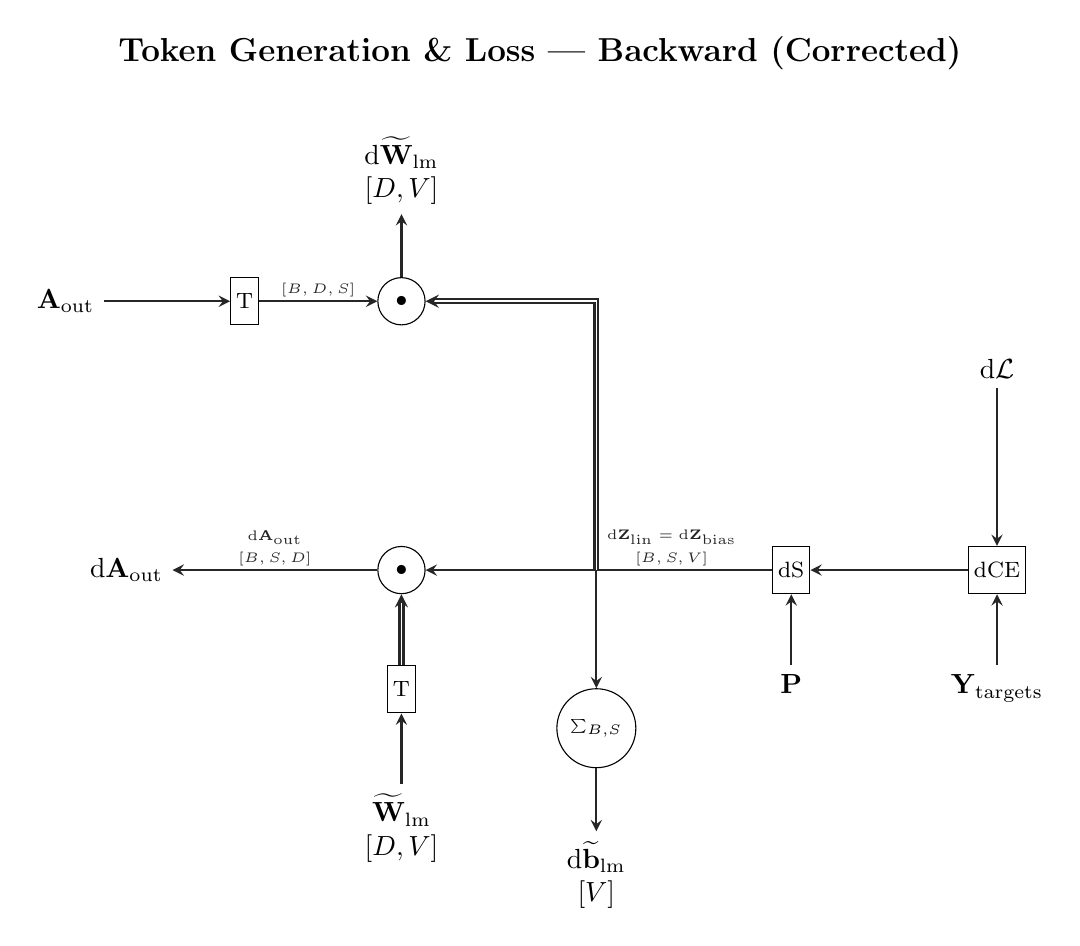
\begin{tikzpicture}[
  >=stealth,
  auxnode/.style={draw, rectangle, fill=white, minimum height=6mm, inner sep=2pt, font=\footnotesize, align=center},
  mulnode/.style={draw, circle, fill=white, minimum size=6mm, font=\footnotesize, align=center},
  addnode/.style={draw, circle, fill=white, minimum size=6mm, font=\footnotesize, align=center},
  sumnode/.style={draw, circle, fill=white, minimum size=6mm, font=\tiny, align=center},
  flow/.style={<-, thick, black!85},
  flow2/.style={double, <-, thick, black!85},
  fwd/.style={->, thick, black!85},
  gradflow/.style={->, thick, black!85},
  dimlabel/.style={font=\tiny, inner sep=1pt, align=center}
]

% Start from dL
\node           (dL)    at (18,0) {$\text{d}\mathcal{L}$};
\node[auxnode]  (dCE)   [below=2.0cm of dL] {dCE};
\node           (Y)     [below=0.9cm of dCE] {$\mathbf{Y_\text{targets}}$};

% Softmax backward
\node[auxnode]  (dS)   [left=2.0cm of dCE] {dS};
\node           (P)     [below=0.9cm of dS] {$\mathbf{P}$};

% Logits (Linear Projection) backprop node
\node[mulnode]  (backMul) [left=4.4cm of dS] {$\bullet$};
\node[auxnode]  (T_Wlm)   [below=0.9cm of backMul] {T};
\node           (Wlm)     [align=center, below=0.9cm of T_Wlm] {$\widetilde{\mathbf{W}}_{\text{lm}}$\\$[D,V]$};

\coordinate (B_split) at ($(backMul)!0.5!(dS)$);

% SUM node for Bias gradient
\node[sumnode]  (SumB) [below=1.5cm of B_split] {$\sum_{B,S}$};
\node           (db)   [align=center, below=0.8cm of SumB] {$\text{d}\widetilde{\mathbf{b}}_{\text{lm}}$\\$[V]$};

% dW calc
\node[mulnode]  (dWmul) [above=2.8cm of backMul] {$\bullet$};
\node[auxnode]  (TAout) [left=1.5cm of dWmul] {T};
\node           (Aout)  [left=1.6cm of TAout] {$\mathbf{A}_{\text{out}}$};
\node           (dW)    [align=center, above=0.8cm of dWmul] {$\text{d}\widetilde{\mathbf{W}}_{\text{lm}}$\\$[D,V]$};

% Back to Transformer
\node           (dH)    [left=2.6cm of backMul] {$\text{d}\mathbf{A}_{\text{out}}$};

% Flows
\draw[flow] (dCE) -- (dL);
\draw[fwd]  (Y) -- (dCE);
\draw[flow] (dS) -- (dCE);
\draw[fwd]  (P) -- (dS);

% Bias grad
\draw[gradflow] (B_split) -- (SumB.north);
\draw[gradflow] (SumB) -- (db);

% Linear projection backprop
\draw[flow] (backMul) -- (dS)
  node[dimlabel, pos=0.71, above]{\shortstack{$\text{d}\mathbf{Z}_{\text{lin}}=\text{d}\mathbf{Z}_{\text{bias}}$\\$[B,S,V]$}};
\draw[flow2] (backMul) -- (T_Wlm);
\draw[fwd]   (Wlm) -- (T_Wlm);
\draw[flow]  (dH) -- (backMul) node[dimlabel, midway, above]{\shortstack{$\text{d}\mathbf{A}_{\text{out}}$\\$[B,S,D]$}};

% dW calculation
\draw[gradflow] (dWmul) -- (dW);
\draw[fwd]  (Aout) -- (TAout);
\draw[fwd]  (TAout) -- (dWmul) node[dimlabel, midway, above]{\shortstack{$[B,D,S]$}};
\draw[flow2] (dWmul) -| (B_split);

\node[font=\large\bfseries, anchor=south]
  at ([yshift=6mm]current bounding box.north) {Token Generation \& Loss — Backward (Corrected)};
\end{tikzpicture}%
}

  \caption{Output projection backward pass. Gradients from the loss are
  propagated through cross-entropy and softmax to the logits, then through
  the language model projection to produce
  $\mathrm{d}\mathbf{A}_{\text{out}}$ and parameter gradients
  $\mathrm{d}\mathbf{W}_{\text{lm}}$ and $\mathrm{d}\mathbf{b}_{\text{lm}}$.}
  \label{fig:single_node_output_backward}
\end{figure}


\fi
\clearpage

% ==========================================================
% 6. Tensor Parallelism (TP)
% ==========================================================
\ifkorean
  % ==========================================================
% 6. 텐서 병렬화 (TP)
% ==========================================================
\section{텐서 병렬화}
\label{sec:tp}

텐서 병렬화에서는 각 레이어의 파라미터를 하나 이상의 텐서 차원을 따라
여러 디바이스에 나누어 저장한다. 모든 디바이스에 동일한 가중치 행렬 전체를
복제하는 대신, 각 디바이스는 가중치의 일부(shard)만을 보유하고,
그에 대응되는 활성값의 일부에 대해서만 연산을 수행한다.
이후 집합 통신(예: All-Reduce, All-Gather)을 사용하여
이 부분 결과들을 모아, Section~\ref{sec:sn}에서 정의한
단일 노드 모델과 동일한 모양의 텐서를 복원한다.

텐서 병렬도의 크기를 $N_T$로 두고,
디바이스 인덱스는 $t \in \{0,\dots,N_T-1\}$로 표기한다.
이 장에서는 Section~\ref{sec:sn}에서의 단일 노드 계산을
이들 $N_T$개 디바이스로 어떻게 나누어 담는지에 초점을 맞춘다.

\textbf{핵심 아이디어는 다음과 같다.}
\begin{itemize}
  \item 큰 가중치 행렬은 행 또는 열 방향으로 나누어,
        각 디바이스가 전체 행렬 $W$ 대신 부분 행렬 $W^{(t)}$만 가지도록 한다.
  \item 각 디바이스는 자신이 가진 부분 가중치와 부분 활성값만을 사용해
        \emph{지역(local) 부분 결과}를 계산한다.
  \item 집합 통신(All-Reduce, All-Gather 등)을 통해
        각 디바이스의 부분 결과를 모아,
        단일 노드 계산 그래프에서 나타나는 것과 동일한 텐서를 재구성한다.
  \item 역전파는 순전파에서의 분할 및 통신 패턴을 그대로 따라가며,
        파라미터와 입력에 대한 기울기가 올바르게 합산되도록 한다.
  \item 디바이스당 메모리 사용량은 대략 $N_T$배 감소하지만,
        각 “글로벌” 행렬 곱은 적어도 한 번의 집합 통신을 필요로 한다.
\end{itemize}

\subsection{텐서 병렬 분할 개요}

큰 그림에서 보면, 텐서 병렬화는 Section~\ref{sec:sn}에서 등장하는
모든 큰 행렬 곱을, 여러 디바이스에서 병렬로 수행되는
작은 행렬 곱들의 집합으로 바꾸는 것으로 볼 수 있다.
선형 레이어
\[
  \mathbf{Y} = \mathbf{X} W + \mathbf{b}, \qquad
  \mathbf{X} \in \mathbb{R}^{B \times D_{\text{in}}},\;
  W \in \mathbb{R}^{D_{\text{in}} \times D_{\text{out}}}
\]
를 분할하는 기본 패턴은 두 가지이다.

\begin{itemize}
  \item \textbf{컬럼 병렬(출력 축 분할) 선형}:
        출력 차원을 기준으로 $W$를 쪼개어
        $W = [W^{(0)},\dots,W^{(N_T-1)}]$,
        $W^{(t)} \in \mathbb{R}^{D_{\text{in}} \times D_{\text{out}}^{(t)}}$
        로 둔다.
        각 디바이스는
        \[
          \mathbf{Y}^{(t)} = \mathbf{X} W^{(t)} + \mathbf{b}^{(t)}
        \]
        를 계산하고, 전체 출력은 단순히 이어 붙여 얻는다:
        \[
          \mathbf{Y} = \mathrm{Concat}_t \mathbf{Y}^{(t)}.
        \]
        순전파 경로에서는 별도의 집합 통신이 필요 없지만,
        이후 레이어에서 이 분할된 축을 다시 모으거나(All-Gather),
        합산(All-Reduce)해야 할 수도 있다.
  \item \textbf{로우 병렬(입력 축 분할) 선형}:
        입력 차원을 기준으로 $W$를 나누고,
        활성값 $\mathbf{X}$도 같은 방식으로 분할한다.
        각 디바이스는 $\mathbf{X}^{(t)}$와 $W^{(t)}$를 가지고 있으며,
        \[
          W^{(t)} \in \mathbb{R}^{D_{\text{in}}^{(t)} \times D_{\text{out}}},
          \qquad
          \mathbf{Y}^{(t)} = \mathbf{X}^{(t)} W^{(t)}
        \]
        를 계산한다.
        이후 $t$에 대한 All-Reduce를 통해 전체 출력을 얻는다:
        \[
          \mathbf{Y} = \sum_{t=0}^{N_T-1} \mathbf{Y}^{(t)}.
        \]
\end{itemize}

트랜스포머 내부에서는 이 두 패턴을 적절히 조합하여,
대부분의 연산이 각 디바이스 로컬로 유지되도록 하고,
레이어당 필요한 All-Reduce/All-Gather 호출 수를 최소화한다.
이러한 스킴을 단일 트랜스포머 블록에 적용한 개략적인 구조는
Figure~\ref{fig:tp_overall_flow}에 나와 있으며,
단일 노드 개요 그림(Figure~\ref{fig:single_node_overall})와 비교해서
보면 이해하기 쉽다.

\begin{figure}[htbp]
  \centering
  \resizebox{\linewidth}{!}{%
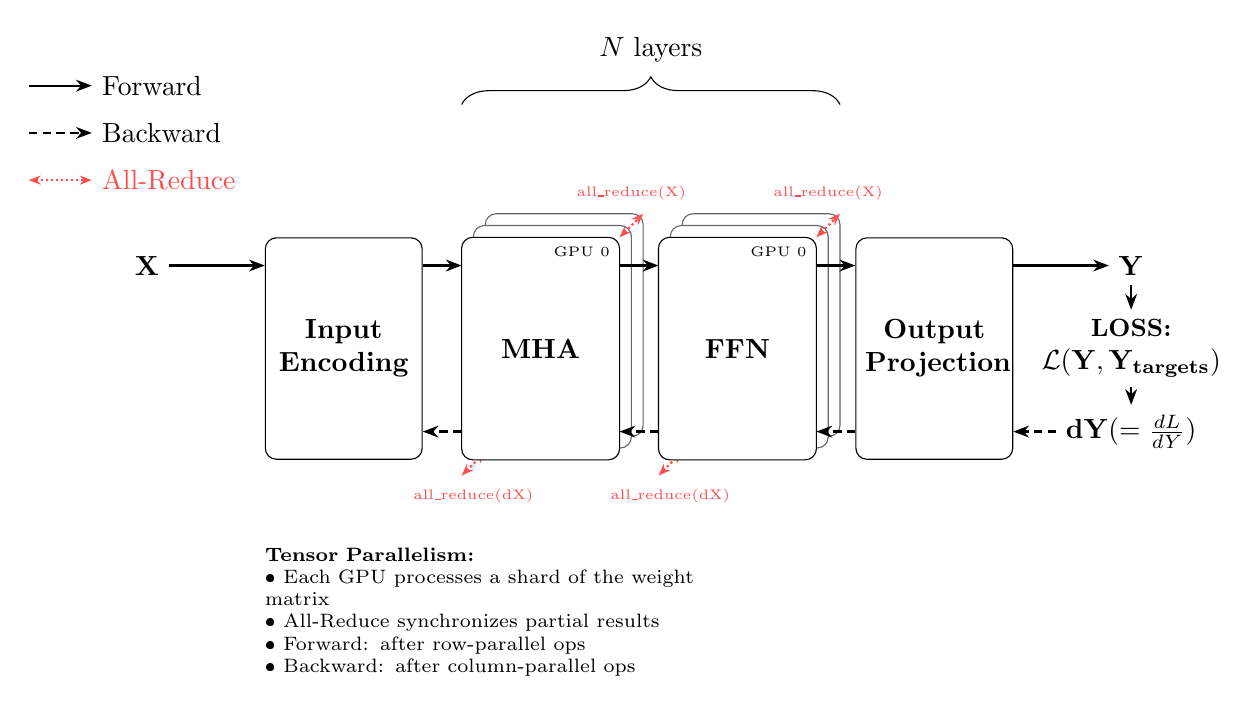
\begin{tikzpicture}[
    node distance=2.5cm,
    >=stealth,
    block/.style={rectangle, draw=black, fill=white, text width=5em, text centered, rounded corners, minimum height=8em, font=\bfseries},
    blockstack/.style={rectangle, draw=black!60, fill=white, text width=5em, text centered, rounded corners, minimum height=8em},
    forward/.style={-{Stealth[length=2mm]}, thick, black},
    backward/.style={-{Stealth[length=2mm]}, thick, black, densely dashed},
    allreduce/.style={{Stealth[length=1.5mm]}-{Stealth[length=1.5mm]}, thick, red!70, densely dotted},
    io/.style={text centered, font=\bfseries}
]
    % Title
    % \node[font=\Large\bfseries] at (10, 6) {Transformer Overall Flow (TP with 3 GPUs)};

    % Forward path nodes (horizontal)
    \node (input) [io] {$\mathbf{X}$};
    \node (encoding) [block, right of=input, yshift=-3em] {Input\\Encoding};

    % MHA blocks (3 stacked) - GPU 2 (back)
    \node (mha3) [blockstack, right of=encoding, xshift=0.3cm, yshift=0.3cm] {};
    % MHA blocks (3 stacked) - GPU 1 (middle)
    \node (mha2) [blockstack, right of=encoding, xshift=0.15cm, yshift=0.15cm] {};
    % MHA blocks (3 stacked) - GPU 0 (front)
    \node (mha) [block, right of=encoding] {MHA};

    % Small GPU labels for MHA
    \node[font=\tiny, anchor=north east] at (mha.north east) {GPU 0};

    % FFN blocks (3 stacked) - GPU 2 (back)
    \node (mlp3) [blockstack, right of=mha, xshift=0.3cm, yshift=0.3cm] {};
    % FFN blocks (3 stacked) - GPU 1 (middle)
    \node (mlp2) [blockstack, right of=mha, xshift=0.15cm, yshift=0.15cm] {};
    % FFN blocks (3 stacked) - GPU 0 (front)
    \node (mlp) [block, right of=mha] {FFN};

    % Small GPU labels for FFN
    \node[font=\tiny, anchor=north east] at (mlp.north east) {GPU 0};

    \node (output) [block, right of=mlp] {Output\\Projection};
    \node (pred) [io, right of=output, yshift=3em] {$\mathbf{Y}$};
    \node (loss) [align=center, io, right of=output] {\small LOSS:\\$\mathcal{L}(\mathbf{Y,Y_\text{targets}})$};
    \node (gradient) [io, right of=output, yshift=-3em] {$\mathbf{dY}(=\frac{dL}{dY})$};

    % All-Reduce arrows (Backward drawn first, then blocks, then Forward on top)
    % Backward All-Reduce - FFN (left-bottom corner, lower position)
    \draw [allreduce] ([yshift=-0.2cm]mlp.south west) -- ([xshift=0.3cm, yshift=0.1cm]mlp.south west);
    \node[font=\tiny, red!70, anchor=north] at ([xshift=0.15cm, yshift=-0.25cm]mlp.south west) {all\_reduce(dX)};

    % Backward All-Reduce - MHA (left-bottom corner, lower position)
    \draw [allreduce] ([yshift=-0.2cm]mha.south west) -- ([xshift=0.3cm, yshift=0.1cm]mha.south west);
    \node[font=\tiny, red!70, anchor=north] at ([xshift=0.15cm, yshift=-0.25cm]mha.south west) {all\_reduce(dX)};

    % Redraw blocks to cover backward All-Reduce arrows
    \draw [draw=black!60, fill=white, rounded corners] (mha3.south west) rectangle (mha3.north east);
    \draw [draw=black!60, fill=white, rounded corners] (mha2.south west) rectangle (mha2.north east);
    \draw [draw=black, fill=white, rounded corners, line width=0.4pt] (mha.south west) rectangle (mha.north east);
    \node[font=\bfseries] at (mha.center) {MHA};
    \node[font=\tiny, anchor=north east] at (mha.north east) {GPU 0};

    \draw [draw=black!60, fill=white, rounded corners] (mlp3.south west) rectangle (mlp3.north east);
    \draw [draw=black!60, fill=white, rounded corners] (mlp2.south west) rectangle (mlp2.north east);
    \draw [draw=black, fill=white, rounded corners, line width=0.4pt] (mlp.south west) rectangle (mlp.north east);
    \node[font=\bfseries] at (mlp.center) {FFN};
    \node[font=\tiny, anchor=north east] at (mlp.north east) {GPU 0};

    % Forward All-Reduce - MHA (right-top corner) - drawn after blocks to appear on top
    \draw [allreduce] (mha.north east) -- ([xshift=0.3cm, yshift=0.3cm]mha.north east);
    \node[font=\tiny, red!70, anchor=south] at ([xshift=0.15cm, yshift=0.35cm]mha.north east) {all\_reduce(X)};

    % Forward All-Reduce - FFN (right-top corner) - drawn after blocks to appear on top
    \draw [allreduce] (mlp.north east) -- ([xshift=0.3cm, yshift=0.3cm]mlp.north east);
    \node[font=\tiny, red!70, anchor=south] at ([xshift=0.15cm, yshift=0.35cm]mlp.north east) {all\_reduce(X)};

    % Forward arrows (upper part of blocks)
    \draw [forward] (input) -- ([yshift=3em]encoding.west);
    \draw [forward] ([yshift=3em]encoding.east) -- ([yshift=3em]mha.west);
    \draw [forward] ([yshift=3em]mha.east) -- ([yshift=3em]mlp.west);
    \draw [forward] ([yshift=3em]mlp.east) -- ([yshift=3em]output.west);
    \draw [forward] ([yshift=3em]output.east) -- (pred);
    \draw [forward] (pred) -- (loss);
    \draw [backward] (loss) -- (gradient);

    % Backward arrows (lower part of blocks)
    \draw [backward] (gradient) -- ([yshift=-3em]output.east);
    \draw [backward] ([yshift=-3em]output.west) -- ([yshift=-3em]mlp.east);
    \draw [backward] ([yshift=-3em]mlp.west) -- ([yshift=-3em]mha.east);
    \draw [backward] ([yshift=-3em]mha.west) -- ([yshift=-3em]encoding.east);

    % Brace for layer repetition (horizontal - using mlp with x offset to match mlp3)
    \draw[decorate, decoration={brace, amplitude=10pt}]
        ([yshift=4.8em]mha.north west) -- ([xshift=0.3cm, yshift=4.8em]mlp.north east)
        node[midway, above=12pt, font=\normalsize] {$N$ layers};

    % Labels (Legend)
    \coordinate (legend) at ([xshift=-1.5cm, yshift=6.5em]input);
    \draw[forward] (legend) -- ++(0.8,0) node[right, font=\normalsize] {Forward};
    \draw[backward] ([yshift=-0.6cm]legend) -- ++(0.8,0) node[right, font=\normalsize] {Backward};
    \draw[allreduce] ([yshift=-1.2cm]legend) -- ++(0.8,0) node[right, font=\normalsize] {All-Reduce};

    % TP explanation
    \node[font=\scriptsize, align=left, text width=6cm] at ([xshift=2cm, yshift=-5.5em]encoding.south) {
        \textbf{Tensor Parallelism:}\\
        • Each GPU processes a shard of the weight matrix\\
        • All-Reduce synchronizes partial results\\
        • Forward: after row-parallel ops\\
        • Backward: after column-parallel ops
    };

\end{tikzpicture}%
}
  \caption{텐서 병렬화가 적용된 전체 트랜스포머 레이어.
  단일 노드 모델의 큰 선형 레이어는 $N_T$개의 작은 matmul로 나뉘어
  서로 다른 디바이스에서 실행된다.
  색깔 화살표는 부분 결과를 모으기 위해 집합 통신
  (예: All-Reduce, All-Gather)이 필요한 위치를 나타내고,
  나머지 로컬 계산은 Figure~\ref{fig:single_node_overall}과
  구조적으로 동일하다.}
  \label{fig:tp_overall_flow}
\end{figure}

% ------------------------ 6.1 MHA with Tensor Parallelism -------------
\subsection{텐서 병렬화된 MHA}

이제 텐서 병렬화를 멀티헤드 어텐션(MHA) 블록에 적용해 보자.
Section~\ref{sec:sn}.2에서 보았듯이, 단일 노드의 어텐션 블록은
입력 $\mathbf{X} \in [B,S,D]$를
Q/K/V 프로젝션, 스케일된 내적 어텐션, 출력 프로젝션, 잔차 연결을 통해
$\mathbf{A}_{\text{out}} \in [B,S,D]$로 사상한다.

텐서 병렬화에서는 이 계산을 $N_T$개 디바이스에 다음과 같이 나눈다.
\begin{itemize}
  \item 각 디바이스는 일부 어텐션 헤드, 또는 동등하게
        Q/K/V 프로젝션 출력 채널의 부분 집합만을 담당한다.
  \item softmax와 값(value) 기반 가중합은 각 디바이스가
        자신이 담당하는 헤드에 대해서만 로컬로 계산한다.
  \item 출력 프로젝션은 로우 병렬(입력 분할) 형태로 구현하여,
        각 디바이스의 부분 결과를 All-Reduce로 합산한 뒤,
        단일 노드와 동일한 $\mathbf{A}_{\text{out}}$을 복원한다.
\end{itemize}

\subsubsection{순전파}

입력은 단일 노드와 마찬가지로
\[
  \mathbf{X} \in \mathbb{R}^{B \times S \times D}
\]
이고, $N_H$개의 헤드와 각 헤드 차원 $D_h$에 대해
$D = N_H D_h$를 가정한다.
텐서 병렬화에서는 헤드를 $N_T$ 디바이스에 나누어,
각 디바이스가 $N_H^{(t)}$개 헤드와 차원 $D_h^{(t)}$를 갖도록 한다
(이들의 합이 전체 $N_H$, $D_h$가 되도록).

\paragraph{(1) 정규화와 공유 입력.}
먼저 레이어 정규화를 적용한다.
\[
  \mathbf{X}_{\text{norm}} = \mathrm{LN}(\mathbf{X})
  \in \mathbb{R}^{B \times S \times D}.
\]
$\mathbf{X}_{\text{norm}}$는 텐서 병렬 디바이스 전체에 \emph{공유}되며,
각 디바이스는 동일한 $\mathbf{X}_{\text{norm}}$를 본다.

\paragraph{(2) Q/K/V 컬럼 병렬 프로젝션.}
Q/K/V 프로젝션은 컬럼 병렬 선형으로 구현하여,
각 디바이스가 출력 채널의 일부만 갖도록 한다.
\[
  W_Q = [W_Q^{(0)},\dots,W_Q^{(N_T-1)}], \quad
  W_K = [W_K^{(0)},\dots,W_K^{(N_T-1)}], \quad
  W_V = [W_V^{(0)},\dots,W_V^{(N_T-1)}],
\]
\[
  W_Q^{(t)}, W_K^{(t)}, W_V^{(t)}
  \in \mathbb{R}^{D \times D_{\text{head}}^{(t)}},
\]
와 같이 두면, 각 디바이스는 다음을 계산한다.
\[
  \mathbf{Q}^{(t)} = \mathbf{X}_{\text{norm}} W_Q^{(t)}, \quad
  \mathbf{K}^{(t)} = \mathbf{X}_{\text{norm}} W_K^{(t)}, \quad
  \mathbf{V}^{(t)} = \mathbf{X}_{\text{norm}} W_V^{(t)}.
\]
여기서 $D_{\text{head}}^{(t)}$는 디바이스 $t$가 담당하는
헤드 차원의 총합이다.
헤드 차원을 명시적으로 드러내면,
\[
  \mathbf{Q}^{(t)}, \mathbf{K}^{(t)}, \mathbf{V}^{(t)}
  \in \mathbb{R}^{B \times N_H^{(t)} \times S \times D_h}.
\]

\paragraph{(3) 로컬 스케일드 어텐션.}
각 디바이스는 자신이 담당하는 헤드에 대해서만
스케일된 내적 어텐션을 계산한다.
\[
  \mathbf{S}^{(t)} = \frac{\mathbf{Q}^{(t)} (\mathbf{K}^{(t)})^{\top}}
                           {\sqrt{D_h^{(t)}}},\qquad
  \mathbf{A}_S^{(t)} = \mathrm{Softmax}(\mathrm{Mask}(\mathbf{S}^{(t)})),
\]
\[
  \mathbf{A}_{\text{heads}}^{(t)} = \mathbf{A}_S^{(t)} \mathbf{V}^{(t)}.
\]
이 과정에는 디바이스 간 통신이 필요 없다.

\paragraph{(4) 헤드 결합과 로우 병렬 출력 프로젝션.}
각 디바이스는 자신이 담당하는 헤드들만 모아
\[
  \mathbf{A}_{\text{cat}}^{(t)}
  \in \mathbb{R}^{B \times S \times D^{(t)}}
\]
를 만든다. 이후 출력 프로젝션을 로우 병렬 선형으로 구현한다.
\[
  W_O
    = \begin{bmatrix} W_O^{(0)} \\ \vdots \\ W_O^{(N_T-1)} \end{bmatrix},\qquad
  W_O^{(t)} \in \mathbb{R}^{D^{(t)} \times D}.
\]
각 디바이스는
\[
  \mathbf{A}_{\text{lin}}^{(t)}
    = \mathbf{A}_{\text{cat}}^{(t)} W_O^{(t)} + \mathbf{b}_O^{(t)}
\]
를 계산하고, $t$에 대한 All-Reduce를 통해
\[
  \mathbf{A}_{\text{lin}}
    = \sum_{t=0}^{N_T-1} \mathbf{A}_{\text{lin}}^{(t)}
\]
을 얻는다.
이제 모든 디바이스가 동일한 $\mathbf{A}_{\text{lin}}$을 가지므로,
이후 드롭아웃과 입력 $\mathbf{X}$와의 잔차 연결은
각 디바이스에서 로컬로 적용할 수 있다.

이 순서와 All-Reduce의 위치는
Figure~\ref{fig:mha_forward_tp}에 명시적으로 표시되어 있다.

\begin{landscape}
\begin{figure}[p]
  \centering
  \resizebox{\linewidth}{!}{%
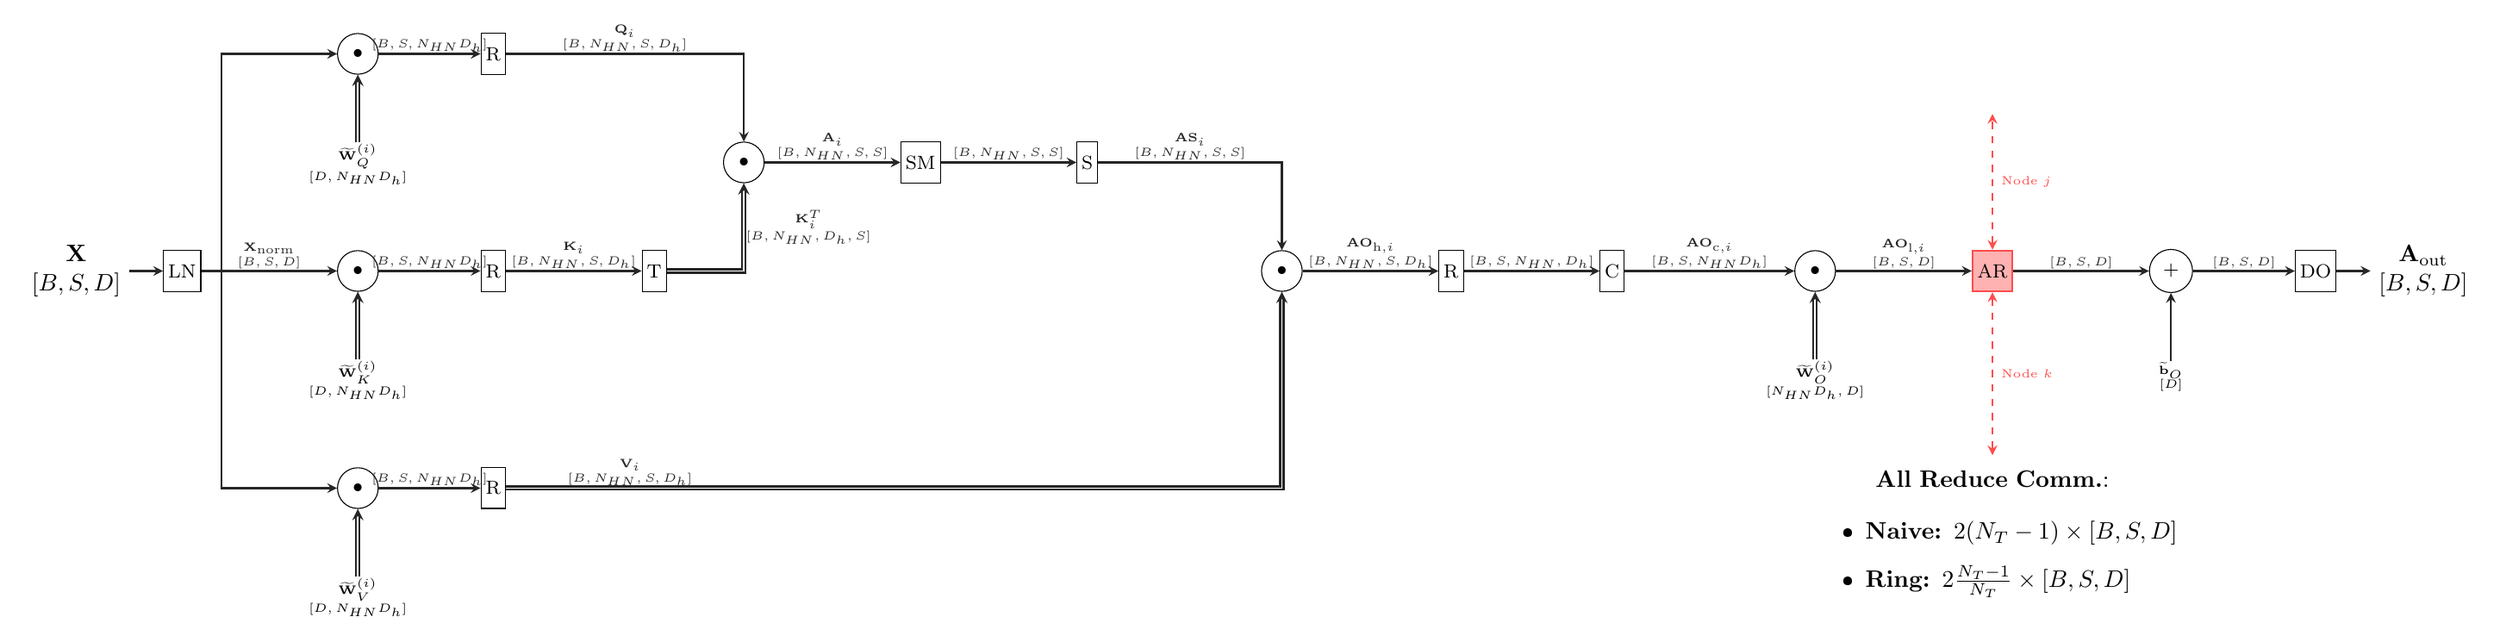
\begin{tikzpicture}[
  every node/.style={transform shape},
  >=stealth,
  auxnode/.style={draw, rectangle, fill=white, minimum height=6mm, inner sep=2pt, font=\footnotesize, align=center},
  mulnode/.style={draw, circle, fill=white, minimum size=6mm, font=\footnotesize, align=center},
  addnode/.style={draw, circle, fill=white, minimum size=6mm, font=\footnotesize, align=center},
  allreduce/.style={draw, rectangle, fill=red!30, minimum height=6mm, inner sep=2pt, font=\footnotesize, align=center, thick, draw=red!70},
  flow/.style={->, thick, black!85},
  flow2/.style={->, double, thick, black!85},
  commflow/.style={<->, thick, red!70, dashed},
  dimlabel/.style={font=\tiny, inner sep=0.5pt, align=center}
]
% \node[font=\Large\bfseries] at (9, 4.5) {Multi-Head Attention Forward Pass (Node $i$)};

\node (Input) at (0.5, 0) [align=center] {$\mathbf{X}$\\$[B,S,D]$};
\node[auxnode] (LN) [right=0.5cm of Input] {LN};

\node[mulnode] (Proj_Q) [right=2.0cm of LN, yshift=3.2cm] {$\bullet$};
\node[auxnode] (R_Q) [right=1.5cm of Proj_Q] {R};

\node[mulnode] (Proj_K) [right=2.0cm of LN, yshift=0cm] {$\bullet$};
\node[auxnode] (R_K) [right=1.5cm of Proj_K] {R};

\node[mulnode] (Proj_V) [right=2.0cm of LN, yshift=-3.2cm] {$\bullet$};
\node[auxnode] (R_V) [right=1.5cm of Proj_V] {R};

\node[dimlabel] (WQ) [align=center, below=1.0cm of Proj_Q] {$\widetilde{\mathbf{W}}_{Q}^{(i)}$\\$[D,N_{HN}D_h]$};
\node[dimlabel] (WK) [align=center, below=1.0cm of Proj_K] {$\widetilde{\mathbf{W}}_{K}^{(i)}$\\$[D,N_{HN}D_h]$};
\node[dimlabel] (WV) [align=center, below=1.0cm of Proj_V] {$\widetilde{\mathbf{W}}_{V}^{(i)}$\\$[D,N_{HN}D_h]$};

\node[auxnode] (T_K) [right=2.0cm of R_K] {T};
\node[mulnode] (QK) [right=3.2cm of R_Q, yshift=-1.6cm] {$\bullet$};
\node[auxnode] (SM) [right=2.0cm of QK] {SM};
\node[auxnode] (Soft) [right=2.0cm of SM] {S};
\node[mulnode] (PV) [right=2.4cm of Soft, yshift=-1.6cm] {$\bullet$};

\node[auxnode] (R_Merge) [right=2.0cm of PV] {R};
\node[auxnode] (Cat) [right=2.0cm of R_Merge] {C};

\node[mulnode] (OProj) [right=2.5cm of Cat] {$\bullet$};
\node[dimlabel] (WO_FWD) [align=center, below=1.0cm of OProj] {$\widetilde{\mathbf{W}}_{O}^{(i)}$\\$[N_{HN}D_h,D]$};
\node[allreduce] (AR) [right=2.0cm of OProj] {AR};
\node[
  align=center,
  below=2.5cm of AR,
  text width=5.5cm % 적당한 값으로 조정
] (AR_info) {%
  \textbf{All Reduce Comm.}:\\[2pt]
  \begin{itemize}
    \item \textbf{Naive:} $2(N_T-1) \times [B,S,D]$
    \item \textbf{Ring:} $2\frac{N_T-1}{N_T} \times [B,S,D]$
  \end{itemize}
};
\node[addnode] (AddB) [right=2.0cm of AR] {+};
\node[dimlabel] (BO) [align=center, below=1.0cm of AddB] {$\widetilde{\mathbf{b}}_{O}$\\$[D]$};
\node[auxnode] (Drop) [right=1.5cm of AddB] {DO};
\node (Aout) [align=center, right=0.5cm of Drop] {$\mathbf{A}_{\text{out}}$\\$[B,S,D]$};

\draw[flow] (Input) -- (LN);

\draw[flow] (LN.east) -- ++(0.3,0) |- (Proj_Q.west);
\draw[flow] (LN) -- (Proj_K.west) node[dimlabel, midway, above]{$\mathbf{X}_{\text{norm}}$\\$[B,S,D]$};
\draw[flow] (LN.east) -- ++(0.3,0) |- (Proj_V.west);

\draw[flow2] (WQ) -- (Proj_Q);
\draw[flow2] (WK) -- (Proj_K);
\draw[flow2] (WV) -- (Proj_V);

\draw[flow] (Proj_Q) -- (R_Q) node[dimlabel, midway, above]{$[B,S,N_{HN}D_h]$};
\draw[flow] (Proj_K) -- (R_K) node[dimlabel, midway, above]{$[B,S,N_{HN}D_h]$};
\draw[flow] (Proj_V) -- (R_V) node[dimlabel, midway, above]{$[B,S,N_{HN}D_h]$};

\draw[flow] (R_Q) -| (QK) node[dimlabel, near start, above]{$\mathbf{Q}_i$\\$[B,N_{HN},S,D_h]$};
\draw[flow] (R_K) -- (T_K) node[dimlabel, midway, above]{$\mathbf{K}_i$\\$[B,N_{HN},S,D_h]$};
\draw[flow2] (T_K) -| (QK) node[dimlabel, near end, right]{$\mathbf{K}_i^{T}$\\$[B,N_{HN},D_h,S]$};

\draw[flow] (QK) -- (SM) node[dimlabel, midway, above]{$\mathbf{A}_i$\\$[B,N_{HN},S,S]$};
\draw[flow] (SM) -- (Soft) node[dimlabel, midway, above]{$[B,N_{HN},S,S]$};
\draw[flow] (Soft) -| (PV) node[dimlabel, near start, above]{$\mathbf{AS}_i$\\$[B,N_{HN},S,S]$};
\draw[flow2] (R_V) -| (PV) node[dimlabel, pos=0.08, above]{$\mathbf{V}_i$\\$[B,N_{HN},S,D_h]$};

\draw[flow] (PV) -- (R_Merge) node[dimlabel, midway, above]{$\mathbf{AO}_{\text{h},i}$\\$[B,N_{HN},S,D_h]$};
\draw[flow] (R_Merge) -- (Cat) node[dimlabel, midway, above]{$[B,S,N_{HN},D_h]$};
\draw[flow] (Cat) -- (OProj) node[dimlabel, midway, above]{$\mathbf{AO}_{\text{c},i}$\\$[B,S,N_{HN}D_h]$};
\draw[flow2] (WO_FWD) -- (OProj);
\draw[flow] (OProj) -- (AR) node[dimlabel, midway, above]{$\mathbf{AO}_{\text{l},i}$\\$[B,S,D]$};

% All-Reduce communication arrows
\draw[commflow] (AR.north) -- ++(0, 2.0) node[midway, right, font=\tiny]{Node $j$};
\draw[commflow] (AR.south) -- ++(0, -2.4) node[midway, right, font=\tiny]{Node $k$};

\draw[flow] (AR) -- (AddB) node[dimlabel, midway, above]{$[B,S,D]$};
\draw[flow] (BO) -- (AddB);
\draw[flow] (AddB) -- (Drop) node[dimlabel, midway, above]{$[B,S,D]$};
\draw[flow] (Drop) -- (Aout);
\end{tikzpicture}%
}
  \caption{텐서 병렬화된 MHA의 순전파.
  Q/K/V 프로젝션은 컬럼 병렬 선형으로 구현되어,
  각 디바이스가 일부 헤드만을 소유한다.
  각 디바이스는 자신이 담당하는 헤드에 대해 어텐션을 로컬로 계산하고,
  헤드 출력들을 합친 뒤, 로우 병렬 출력 프로젝션을 적용한다.
  이후 All-Reduce를 통해 모든 디바이스에서
  단일 노드와 동일한 $\mathbf{A}_{\text{out}}$를 복원한다.}
  \label{fig:mha_forward_tp}
\end{figure}
\end{landscape}

\subsubsection{역전파}

텐서 병렬 MHA의 역전파는
Section~\ref{sec:sn}.2의 단일 노드 역전파와 같은 상위 구조를 따르되,
기울기가 샤딩되어 있고, 집합 통신이 명시적으로 들어간다는 점만 다르다.
각 디바이스에서 $\mathrm{d}\mathbf{A}_{\text{out}}$로부터 시작하여,
다음과 같은 단계가 진행된다.

\begin{itemize}
  \item \textbf{출력 프로젝션 역전파}:
        로우 병렬 출력 프로젝션은
        $\mathrm{d}\mathbf{A}_{\text{lin}}$으로부터
        로컬 기울기 $\mathrm{d}\mathbf{A}_{\text{cat}}^{(t)}$와
        파라미터 기울기 $\mathrm{d}W_O^{(t)}, \mathrm{d}\mathbf{b}_O^{(t)}$를 계산한다.
  \item \textbf{헤드 역전파}:
        각 디바이스는 자신이 담당하는 헤드를 따라 역전파를 수행하여
        $\mathrm{d}\mathbf{V}^{(t)}$, $\mathrm{d}\mathbf{A}_S^{(t)}$를 얻고,
        다시 스케일된 내적 및 소프트맥스 역전파를 통해
        $\mathrm{d}\mathbf{Q}^{(t)}$, $\mathrm{d}\mathbf{K}^{(t)}$를 계산한다.
  \item \textbf{Q/K/V 프로젝션 역전파}:
        컬럼 병렬 Q/K/V 선형 레이어는
        로컬 파라미터 기울기
        $\mathrm{d}W_Q^{(t)}, \mathrm{d}W_K^{(t)}, \mathrm{d}W_V^{(t)}$와
        정규화된 입력에 대한 부분 기울기
        $\mathrm{d}\mathbf{X}_{\text{norm}}^{(t)}$를 계산한다.
  \item \textbf{입력 기울기에 대한 All-Reduce}:
        $\mathbf{X}_{\text{norm}}$는 모든 디바이스에 공유되므로,
        모든 Q/K/V shard에서 나온 기울기를 합산해야 한다:
        \[
          \mathrm{d}\mathbf{X}_{\text{norm}}
            = \sum_{t=0}^{N_T-1} \mathrm{d}\mathbf{X}_{\text{norm}}^{(t)},
        \]
        이는 $t$에 대한 All-Reduce로 구현된다.
  \item \textbf{레이어 정규화 역전파}:
        마지막으로 레이어 정규화 역전파를 통해
        $\mathrm{d}\mathbf{X}_{\text{norm}}$을
        원래 입력 $\mathbf{X}$에 대한 기울기
        $\mathrm{d}\mathbf{X}$로 변환한다.
\end{itemize}

이 과정은 Figure~\ref{fig:mha_backward_tp}에서
전체 계산 그래프로 펼쳐져 있고,
각 All-Reduce/All-Gather의 위치가 명시되어 있다.

\begin{landscape}
\begin{figure}[p]
  % no \centering here to avoid compilation issues
  \par\vspace{1cm}
\noindent
\resizebox{\linewidth}{!}{%
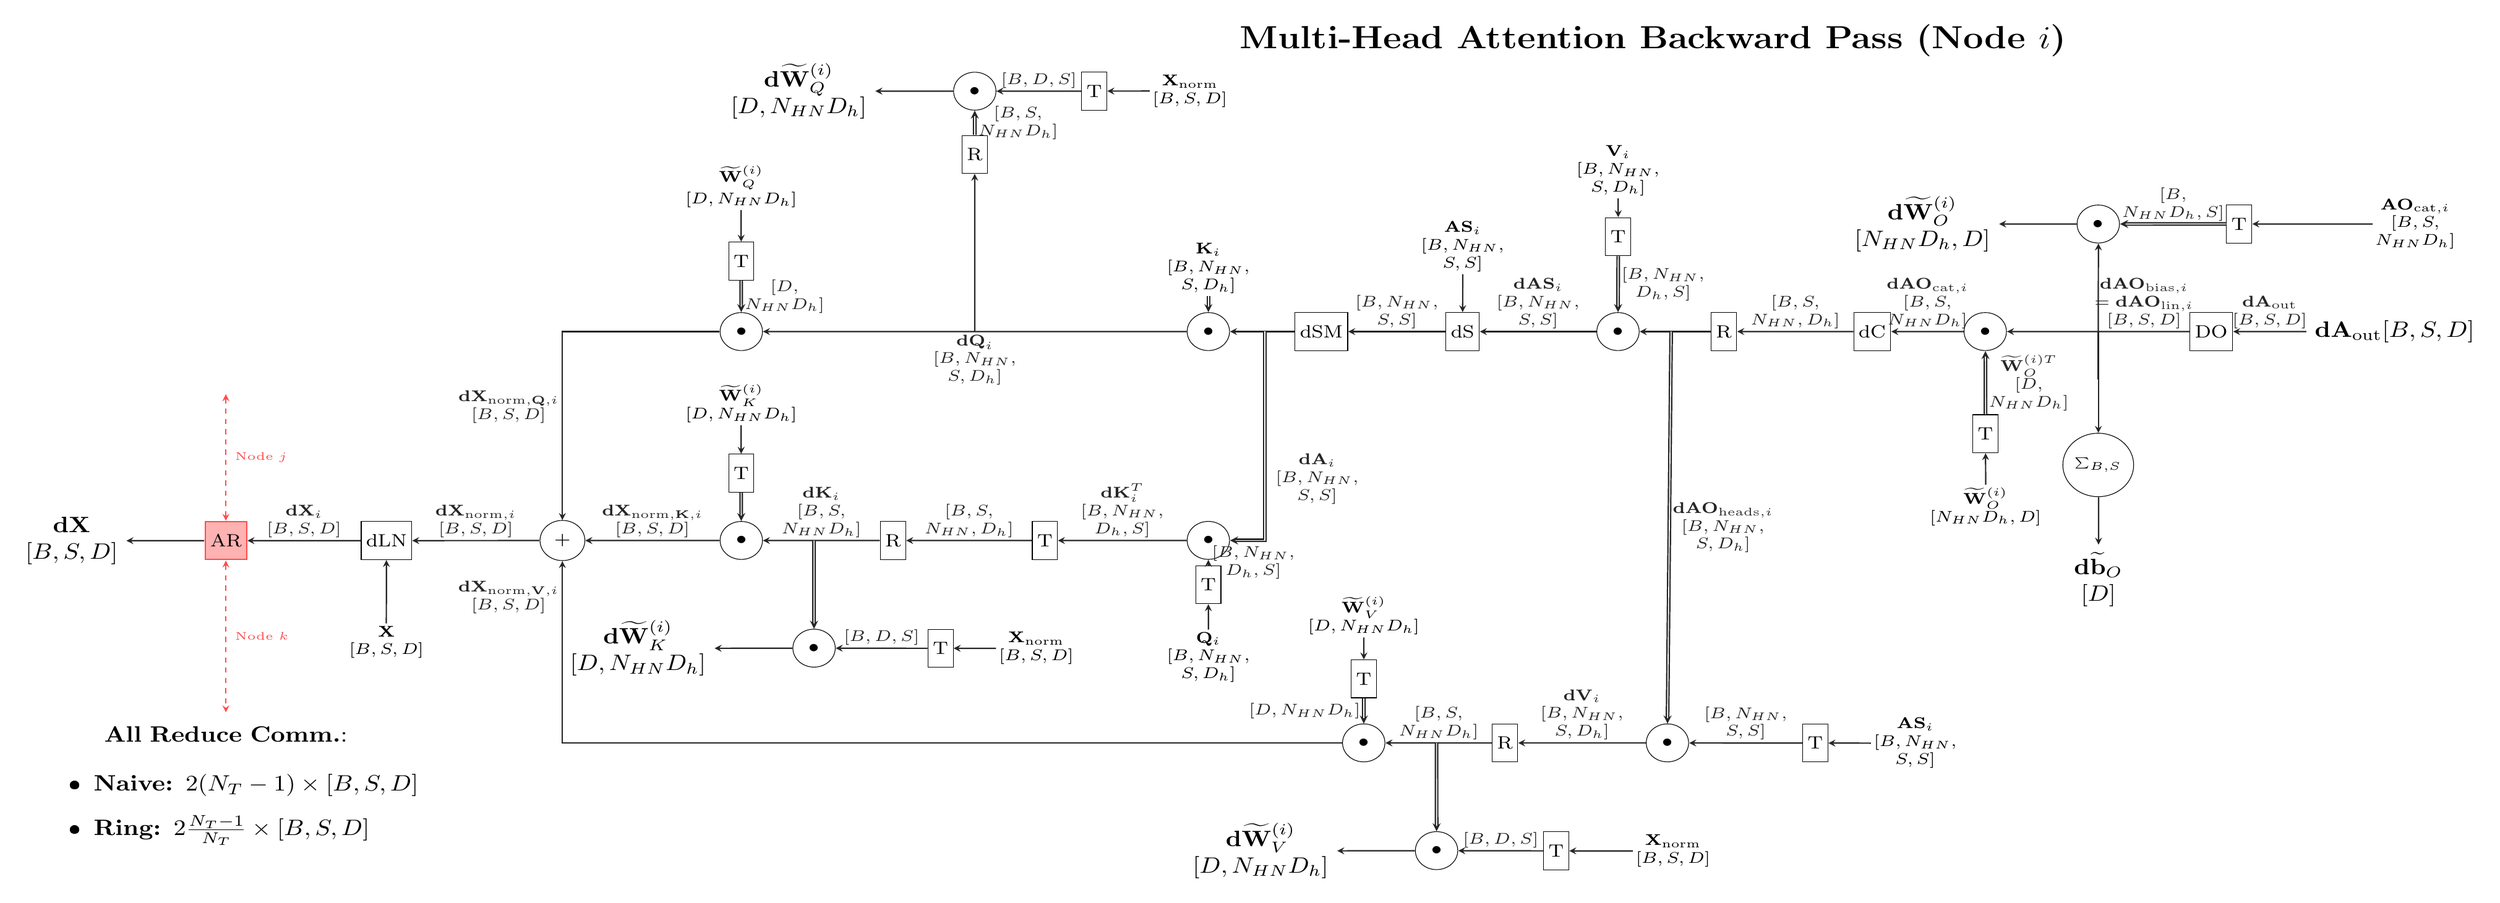
\begin{tikzpicture}[
  every node/.style={transform shape},
  >=stealth,
  auxnode/.style={draw, rectangle, fill=white, minimum height=6mm, inner sep=2pt, font=\footnotesize, align=center},
  mulnode/.style={draw, circle, fill=white, minimum size=6mm, font=\footnotesize, align=center},
  addnode/.style={draw, circle, fill=white, minimum size=6mm, font=\footnotesize, align=center},
  sumnode/.style={draw, circle, fill=white, minimum size=6mm, font=\tiny, align=center},
  allreduce/.style={draw, rectangle, fill=red!30, minimum height=6mm, inner sep=2pt, font=\footnotesize, align=center, thick, draw=red!70},
  flow/.style={->, thick, black!85},
  flow2/.style={->, double, thick, black!85},
  commflow/.style={<->, thick, red!70, dashed},
  dimlabel/.style={font=\scriptsize, inner sep=1pt, align=center},
  gradflow/.style={->, thick, black!85},
  gradweight/.style={->, thick, black!85}
]

\begin{scope}[xscale=1.45, yscale=1.3]

\def\yoffset{-1.0}
\def\dVXyoffset{-6.5}

\coordinate (Grad_Aout_B) at (17.5, \yoffset);
\coordinate (dDrop_center) at (15.9, \yoffset);
\coordinate (ProjGradSplit) at (14.3, \yoffset);
\coordinate (dOProj_center) at (12.7, \yoffset);
\coordinate (C_center) at (11.1, \yoffset);
\coordinate (R_center) at (9.0, \yoffset);
\coordinate (dPV_AS_calc_center) at (7.5, \yoffset);
\coordinate (dSoft_center) at (5.3, \yoffset);
\coordinate (dSM_calc_center) at (3.3, \yoffset);
\coordinate (dV_calc_center) at (8.2, \dVXyoffset+\yoffset);
\coordinate (R_V_bwd_center) at (5.9, \dVXyoffset+\yoffset);
\coordinate (dVX_calc_center) at (3.9, \dVXyoffset+\yoffset);
\coordinate (dQK_calc_Q_center) at (1.7, \yoffset);
\coordinate (dQK_calc_K_center) at (1.7, -3.3+\yoffset);
\coordinate (K_BWD_input_center) at (1.7, 1.0+\yoffset);
\coordinate (T_Q_bwd_center) at (1.7, -4.0+\yoffset);

\node[font=\Large\bfseries] at (8, 4.6+\yoffset) {Multi-Head Attention Backward Pass (Node $i$)};

\node (Grad_Aout_B) at (18.5, \yoffset) {$\mathbf{dA}_{\text{out}}$\\$[B,S,D]$};
\node[auxnode] (DO) at (dDrop_center) {DO};
\node[mulnode] (dOProj) at (dOProj_center) {$\bullet$};

\node[auxnode] (T_WO) [below=1.0cm of dOProj] {T};
\node[dimlabel] (WO_BWD) [below=0.5cm of T_WO] {$\widetilde{\mathbf{W}}_{O}^{(i)}$\\$[N_{HN}D_h,D]$};

\node[mulnode] (dWO_calc) at ($(ProjGradSplit)+(0, 1.7)$) {$\bullet$};
\node[align=center, left=1.1cm of dWO_calc]
  (dWO_GRAD) {$\mathbf{d}\widetilde{\mathbf{W}}_{O}^{(i)}$\\$[N_{HN}D_h,D]$};
\node[auxnode] (T_AO_in) [right=1.5cm of dWO_calc] {T};
\node[dimlabel] (AO_in_local_label) [right=1.7cm of T_AO_in] {$\mathbf{AO}_{\text{cat},i}$\\$[B,S,$\\$N_{HN}D_h]$};

\node[auxnode] (C) at (C_center) {dC};
\node[auxnode] (R) at (R_center) {R};

\node[mulnode] (dPV_AS_calc) at (dPV_AS_calc_center) {$\bullet$};
\node[auxnode] (dSoft) at (dSoft_center) {dS};
\node[auxnode] (dSM_calc) at (dSM_calc_center) {dSM};

\node[mulnode] (dQK_calc_Q) at (dQK_calc_Q_center) {$\bullet$};
\node[mulnode] (dQX_proj_calc) [left=6.0cm of dQK_calc_Q] {$\bullet$};

\node[mulnode] (dQK_calc_K) at (dQK_calc_K_center) {$\bullet$};
\node[mulnode] (dKX_proj_calc) [left=6.0cm of dQK_calc_K] {$\bullet$};

\node[dimlabel] (K_BWD_input) at (K_BWD_input_center) {$\mathbf{K}_i$\\$[B,N_{HN},$\\$S,D_h]$};
\node[auxnode] (T_Q_bwd) at (T_Q_bwd_center) {T};
\node[dimlabel] (Q_BWD_input) [below=0.4cm of T_Q_bwd] {$\mathbf{Q}_i$\\$[B,N_{HN},$\\$S,D_h]$};

\node[dimlabel] (V_FWD) [above=1.8cm of dPV_AS_calc] {$\mathbf{V}_i$\\$[B,N_{HN},$\\$S,D_h]$};
\node[auxnode] (T_V_bwd) [below=0.3cm of V_FWD] {T};

\node[mulnode] (dV_calc) at (dV_calc_center) {$\bullet$};
\node[auxnode] (T_AS_bwd) [right=1.6cm of dV_calc] {T};
\node[dimlabel] (AS_BWD_for_V) [right=0.6cm of T_AS_bwd] {$\mathbf{AS}_i$\\$[B,N_{HN},$\\$S,S]$};

\node[auxnode] (R_V_bwd) at (R_V_bwd_center) {R};
\node[mulnode] (dVX_calc) at (dVX_calc_center) {$\bullet$};

\node[auxnode] (T_WV) [above=0.4cm of dVX_calc] {T};
\node[dimlabel] (WV_BWD) [above=0.35cm of T_WV] {$\widetilde{\mathbf{W}}_{V}^{(i)}$\\$[D,N_{HN}D_h]$};

\node[sumnode] (Sum_dBO) [below=1.6cm of ProjGradSplit] {$\sum_{B, S}$};
\node (dBO) [align=center, below=0.75cm of Sum_dBO] {$\mathbf{d}\widetilde{\mathbf{b}}_{O}$\\$[D]$};

\draw[gradflow] (Grad_Aout_B) -- (DO)
  node[dimlabel, midway, above]{$\mathbf{dA}_{\text{out}}$\\$[B,S,D]$};

\draw[gradflow] (DO) -- (dOProj)
  node[dimlabel, pos=0.25, above]{$\mathbf{dAO}_{\text{bias},i}$\\$=\mathbf{dAO}_{\text{lin},i}$\\$[B,S,D]$};

\draw[gradflow] (ProjGradSplit) -- (dWO_calc.south);
\draw[gradflow] (ProjGradSplit) -- ([yshift=-0.75cm]ProjGradSplit) -| (Sum_dBO.north);

\draw[gradflow] (dOProj) -- (C)
  node[dimlabel, midway, above]{$\mathbf{dAO}_{\text{cat},i}$\\$[B,S,$\\$N_{HN}D_h]$};
\draw[gradflow] (C) -- (R)
  node[dimlabel, midway, above]{$[B,S,$\\$N_{HN},D_h]$};

\coordinate (R_split_point) at ($(dPV_AS_calc)!0.5!(R)$);
\draw[gradflow] (R.west) -- (dPV_AS_calc.east);
\draw[flow2] (R_split_point) -- (dV_calc.north)
  node[dimlabel, midway, right]{$\mathbf{dAO}_{\text{heads},i}$\\$[B,N_{HN},$\\$S,D_h]$};

\draw[gradflow] (V_FWD.south) -- (T_V_bwd.north);
\draw[flow2] (T_V_bwd.south) -- (dPV_AS_calc.north)
  node[dimlabel, midway, right]{$[B,N_{HN},$\\$D_h,S]$};
\draw[gradflow] (dPV_AS_calc.west) -- (dSoft.east)
  node[dimlabel, midway, above]{$\mathbf{dAS}_i$\\$[B,N_{HN},$\\$S,S]$};

\node (AS_BWD_dS) [dimlabel, above=0.6cm of dSoft] {$\mathbf{AS}_i$\\$[B,N_{HN},$\\$S,S]$};
\draw[gradflow] (AS_BWD_dS.south) -- (dSoft.north);
\draw[gradflow] (dSoft.west) -- (dSM_calc.east)
  node[dimlabel, midway, above]{$[B,N_{HN},$\\$S,S]$};

\coordinate (dA_Split_X) at ($(dSM_calc_center)!0.5!(dQK_calc_Q_center)$);
\coordinate (dA_Split) at (dA_Split_X |- dQK_calc_Q.east);
\draw[gradflow] (dSM_calc.west) -- (dQK_calc_Q.east);
\draw[flow2] (dA_Split) -- (dA_Split |- dQK_calc_K.east) -- (dQK_calc_K.east)
  node[dimlabel, pos=-1.5, above, yshift=15]{$\mathbf{dA}_i$\\$[B,N_{HN},$\\$S,S]$};

\draw[flow2] (K_BWD_input.south) -- (dQK_calc_Q.north);
\draw[gradweight] (dQK_calc_Q) -- (dQX_proj_calc)
  node[dimlabel, midway, below]{$\mathbf{dQ}_i$\\$[B,N_{HN},$\\$S,D_h]$};

\node[auxnode] (T_WQ_bwd) [above=0.5cm of dQX_proj_calc] {T};
\node[dimlabel] (WQ_bwd) [above=0.5cm of T_WQ_bwd] {$\widetilde{\mathbf{W}}_{Q}^{(i)}$\\$[D,N_{HN}D_h]$};
\draw[flow] (WQ_bwd) -- (T_WQ_bwd);
\draw[flow2] (T_WQ_bwd.south) -- (dQX_proj_calc.north)
  node[dimlabel, midway, right]{$[D,$\\$N_{HN}D_h]$};

\draw[flow] (Q_BWD_input.north) -- (T_Q_bwd.south);
\draw[flow] (T_Q_bwd.north) -- (dQK_calc_K.south)
  node[dimlabel, pos=0.55, right]{$[B,N_{HN},$\\$D_h,S]$};

\node[auxnode] (T_dK) at ($(dQK_calc_K)!0.35!(dKX_proj_calc)$) {T};
\node[auxnode] (R_dK_mid) at ($(T_dK)!0.5!(dKX_proj_calc)$) {R};

\draw[gradweight] (dQK_calc_K) -- (T_dK)
  node[dimlabel, midway, above]{$\mathbf{dK}_i^T$\\$[B,N_{HN},$\\$D_h,S]$};
\draw[gradweight] (T_dK) -- (R_dK_mid)
  node[dimlabel, midway, above]{$[B,S,$\\$N_{HN},D_h]$};
\draw[gradweight] (R_dK_mid) -- (dKX_proj_calc)
  node[dimlabel, midway, above]{$\mathbf{dK}_i$\\$[B,S,$\\$N_{HN}D_h]$};

\node[auxnode] (T_WK_bwd) [above=0.45cm of dKX_proj_calc] {T};
\node[dimlabel] (WK_bwd) [above=0.45cm of T_WK_bwd] {$\widetilde{\mathbf{W}}_{K}^{(i)}$\\$[D,N_{HN}D_h]$};
\draw[gradflow] (WK_bwd) -- (T_WK_bwd);
\draw[flow2] (T_WK_bwd.south) -- (dKX_proj_calc.north);

\draw[gradflow] (AS_BWD_for_V.west) -- (T_AS_bwd.east);
\draw[gradflow] (T_AS_bwd.west) -- (dV_calc.east)
  node[dimlabel, midway, above]{$[B,N_{HN},$\\$S,S]$};
\draw[gradflow] (dV_calc.west) -- (R_V_bwd.east)
  node[dimlabel, midway, above]{$\mathbf{dV}_i$\\$[B,N_{HN},$\\$S,D_h]$};
\draw[gradflow] (R_V_bwd) -- (dVX_calc.east)
  node[dimlabel, midway, above]{$[B,S,$\\$N_{HN}D_h]$};

\draw[gradflow] (WV_BWD) -- (T_WV);
\draw[flow2] (T_WV) -- (dVX_calc.north)
  node[dimlabel, midway, left]{$[D,N_{HN}D_h]$};

\node[addnode] (Sum_dXnorm) [left=1.9cm of dKX_proj_calc] {$+$};

\draw[gradweight] (dQX_proj_calc.west) -| node[dimlabel, pos=0.7, left]{$\mathbf{dX}_{\text{norm},\mathbf{Q},i}$\\$[B,S,D]$} (Sum_dXnorm.north);
\draw[gradweight] (dKX_proj_calc.west) -- node[dimlabel, midway, above]{$\mathbf{dX}_{\text{norm},\mathbf{K},i}$\\$[B,S,D]$} (Sum_dXnorm.east);
\draw[gradweight] (dVX_calc.west) -| node[dimlabel, pos=0.9, left]{$\mathbf{dX}_{\text{norm},\mathbf{V},i}$\\$[B,S,D]$} (Sum_dXnorm.south);

\coordinate (dV_branch) at ($(R_V_bwd.west)!0.52!(dVX_calc.east)$);
\node[mulnode] (dWV_mul) at ($(dV_branch)+(0,-1.7cm)$) {$\bullet$};
\draw[flow2] (dV_branch) -- (dWV_mul.north);

\node[auxnode] (T_Xnorm) [right=1.2cm of dWV_mul] {T};
\node[dimlabel] (Xnorm_local) [right=0.9cm of T_Xnorm] {$\mathbf{X}_{\text{norm}}$\\$[B,S,D]$};
\draw[gradflow] (Xnorm_local) -- (T_Xnorm);
\draw[gradflow] (T_Xnorm.west) -- (dWV_mul.east)
  node[dimlabel, midway, above]{$[B,D,S]$};
\node (dWV_out) [align=center, left=1.1cm of dWV_mul] {$\mathbf{d}\widetilde{\mathbf{W}}_{V}^{(i)}$\\$[D,N_{HN}D_h]$};
\draw[gradweight] (dWV_mul.west) -- (dWV_out);

\coordinate (dQ_branch) at ($(dQK_calc_Q.east)!0.50!(dQX_proj_calc.west)$);
\node[mulnode] (dWQ_mul) at ($(dQ_branch)+(0,3.8cm)$) {$\bullet$};
\node[auxnode] (R_dQ_for_WQ) at ($(dWQ_mul)+(0,-1.0cm)$) {R};
\draw[gradflow]  (dQ_branch) -- (R_dQ_for_WQ.south);
\draw[flow2] (R_dQ_for_WQ.north) -- (dWQ_mul.south)
  node[dimlabel, midway, right]{$[B,S,$\\$N_{HN}D_h]$};

\node[auxnode] (T_XnormQ) [right=1.2cm of dWQ_mul] {T};
\node[dimlabel] (Xnorm_localQ) [right=0.6cm of T_XnormQ] {$\mathbf{X}_{\text{norm}}$\\$[B,S,D]$};
\draw[gradflow] (Xnorm_localQ) -- (T_XnormQ);
\draw[gradflow] (T_XnormQ.west) -- (dWQ_mul.east)
  node[dimlabel, midway, above]{$[B,D,S]$};
\node (dWQ_out) [align=center, left=1.1cm of dWQ_mul] {$\mathbf{d}\widetilde{\mathbf{W}}_{Q}^{(i)}$\\$[D,N_{HN}D_h]$};
\draw[gradweight] (dWQ_mul.west) -- (dWQ_out);

\coordinate (dK_branch) at ($(R_dK_mid)!0.52!(dKX_proj_calc)$);
\node[mulnode] (dWK_mul) at ($(dK_branch)+(0,-1.7cm)$) {$\bullet$};
\draw[flow2]  (dK_branch) -- (dWK_mul.north);

\node[auxnode] (T_XnormK) [right=1.3cm of dWK_mul] {T};
\node[dimlabel, right=0.6cm of T_XnormK] (Xnorm_localK) {$\mathbf{X}_{\text{norm}}$\\$[B,S,D]$};
\draw[gradflow] (Xnorm_localK) -- (T_XnormK);
\draw[gradflow] (T_XnormK.west) -- (dWK_mul.east)
  node[dimlabel, midway, above]{$[B,D,S]$};
\node (dWK_out) [align=center, left=1.1cm of dWK_mul] {$\mathbf{d}\widetilde{\mathbf{W}}_{K}^{(i)}$\\$[D,N_{HN}D_h]$};
\draw[gradweight] (dWK_mul.west) -- (dWK_out);

\draw[gradweight] (Sum_dBO) -- (dBO);

\draw[gradflow] (WO_BWD) -- (T_WO);
\draw[flow2] (T_WO) -- (dOProj)
  node[dimlabel, midway, right]{$\widetilde{\mathbf{W}}_{O}^{(i)T}$\\$[D,$\\$N_{HN}D_h]$};
\draw[gradflow] (AO_in_local_label) -- (T_AO_in);
\draw[flow2] (T_AO_in) -- (dWO_calc.east)
  node[dimlabel, midway, above]{$[B,$\\$N_{HN}D_h,S]$};
\draw[gradweight] (dWO_calc) -- (dWO_GRAD);

\node[auxnode] (dLN) [left=1.8cm of Sum_dXnorm] {dLN};
\draw[gradweight] (Sum_dXnorm.west) -- node[dimlabel, midway, above]
  {$\mathbf{dX}_{\text{norm},i}$\\$[B,S,D]$} (dLN.east);

\node[allreduce] (AR) [left=1.6cm of dLN] {AR};
\node[
  align=center,
  below=2.5cm of AR,
  text width=5.5cm
] (AR_info) {%
  \textbf{All Reduce Comm.}:\\[2pt]
  \begin{itemize}
    \item \textbf{Naive:} $2(N_T-1) \times [B,S,D]$
    \item \textbf{Ring:} $2\frac{N_T-1}{N_T} \times [B,S,D]$
  \end{itemize}
};

% All-Reduce communication arrows
\draw[commflow] (AR.north) -- ++(0, 2.0) node[midway, right, font=\tiny]{Node $j$};
\draw[commflow] (AR.south) -- ++(0, -2.4) node[midway, right, font=\tiny]{Node $k$};

\draw[gradweight] (dLN.west) -- (AR.east) node[dimlabel, midway, above]{$\mathbf{dX}_i$\\$[B,S,D]$};

\node (dX_OUT) [align=center, left=1.1cm of AR] {$\mathbf{dX}$\\$[B,S,D]$};
\draw[gradweight] (AR.west) -- (dX_OUT);

\node[dimlabel] (LNCache) [below=1.0cm of dLN] {$\mathbf{X}$\\$[B,S,D]$};
\draw[gradflow] (LNCache.north) -- (dLN.south);

\end{scope}
\end{tikzpicture}
}
  \caption{텐서 병렬화된 MHA의 역전파.
  각 디바이스는 로컬 Q/K/V 프로젝션과 자신이 담당하는
  어텐션 헤드를 따라 역전파를 수행한다.
  정규화된 입력에 대한 기울기는 All-Reduce를 통해 모든 디바이스에서
  합산되며, 파라미터 기울기는 각 shard
  $W_Q^{(t)}, W_K^{(t)}, W_V^{(t)}, W_O^{(t)}$에 대해
  로컬로 누적된다.}
  \label{fig:mha_backward_tp}
\end{figure}
\end{landscape}

% ------------------------ 6.2 MLP with Tensor Parallelism -------------
\subsection{텐서 병렬화된 MLP}

피드포워드(MLP) 블록은 두 개의 선형 레이어를 가지기 때문에,
하나는 컬럼 병렬, 다른 하나는 로우 병렬로 구현하기에 특히 적합하다.
Section~\ref{sec:sn}.3에서 단일 노드 MLP는
$\mathbf{H} \in [B,S,D]$를 $\mathbf{Y} \in [B,S,D]$로 사상하며,
다음과 같은 구조를 가진다.
\[
  \mathbf{Z}_{\text{up}} = \mathbf{H} W_{\text{up}} + \mathbf{b}_{\text{up}},
  \quad \mathbf{U} = \phi(\mathbf{Z}_{\text{up}}),
\]
\[
  \mathbf{Z}_{\text{down}} = \mathbf{U} W_{\text{down}} + \mathbf{b}_{\text{down}},
  \quad \mathbf{Y} = \mathbf{H} + \mathrm{Dropout}(\mathbf{Z}_{\text{down}}),
\]
여기서 $W_{\text{up}} \in \mathbb{R}^{D \times D_{\text{ff}}}$,
$W_{\text{down}} \in \mathbb{R}^{D_{\text{ff}} \times D}$이다.

텐서 병렬화에서는 $\mathbf{H}$가 모든 디바이스에 공유된다고 가정하고,
상향(up) 선형은 컬럼 병렬, 하향(down) 선형은 로우 병렬로 구현한다.

\subsubsection{순전파}

\paragraph{(1) 컬럼 병렬 상향 프로젝션.}
상향 선형 레이어를
\[
  W_{\text{up}} = [W_{\text{up}}^{(0)},\dots,W_{\text{up}}^{(N_T-1)}],\qquad
  W_{\text{up}}^{(t)} \in \mathbb{R}^{D \times D_{\text{ff}}^{(t)}}
\]
로 나눈다.
각 디바이스는 공유 입력 $\mathbf{H}$에 대해
\[
  \mathbf{Z}_{\text{up}}^{(t)}
    = \mathbf{H} W_{\text{up}}^{(t)} + \mathbf{b}_{\text{up}}^{(t)},
  \qquad
  \mathbf{Z}_{\text{up}}^{(t)} \in \mathbb{R}^{B \times S \times D_{\text{ff}}^{(t)}}
\]
를 계산한다.
전체 $\mathbf{Z}_{\text{up}}$는 개념적으로
\[
  \mathbf{Z}_{\text{up}}
    = \mathrm{Concat}_t \mathbf{Z}_{\text{up}}^{(t)}
\]
로 구성되지만, 이후 연산이 헤드/피처 축을 따라 원소별로 작동하는 경우,
실제로는 각 shard만 가지고 있어도 된다.

\paragraph{(2) 로컬 비선형 활성 함수.}
비선형 함수 $\phi$는 각 디바이스에서 shard별로 적용된다.
\[
  \mathbf{U}^{(t)} = \phi(\mathbf{Z}_{\text{up}}^{(t)}).
\]

\paragraph{(3) 로우 병렬 하향 프로젝션.}
하향 선형 레이어는 입력 차원 방향으로 분할한다.
\[
  W_{\text{down}}
    = \begin{bmatrix}
        W_{\text{down}}^{(0)} \\
        \vdots \\
        W_{\text{down}}^{(N_T-1)}
      \end{bmatrix},
  \qquad
  W_{\text{down}}^{(t)} \in \mathbb{R}^{D_{\text{ff}}^{(t)} \times D}.
\]
각 디바이스는 로컬 shard에 대해
\[
  \mathbf{Z}_{\text{down}}^{(t)}
    = \mathbf{U}^{(t)} W_{\text{down}}^{(t)} + \mathbf{b}_{\text{down}}^{(t)}
\]
를 계산한다.
이후 $t$에 대한 All-Reduce를 수행하여 전체 down-projection 출력을 얻는다.
\[
  \mathbf{Z}_{\text{down}}
    = \sum_{t=0}^{N_T-1} \mathbf{Z}_{\text{down}}^{(t)}.
\]

\paragraph{(4) 드롭아웃과 잔차 연결.}
모든 디바이스가 동일한 $\mathbf{Z}_{\text{down}}$와
$\mathbf{H}$를 가지므로, 드롭아웃과 잔차 연결
\[
  \mathbf{Y} = \mathbf{H} + \mathrm{Dropout}(\mathbf{Z}_{\text{down}})
\]
은 각 디바이스에서 로컬로 수행할 수 있다.

이 전체 순서는 Figure~\ref{fig:mlp_forward_tp}에 요약되어 있으며,
순전파 경로에서 유일한 집합 통신은
down-projection 이후의 All-Reduce이다.

\begin{figure}[htbp]
  \centering
  \resizebox{\linewidth}{!}{%
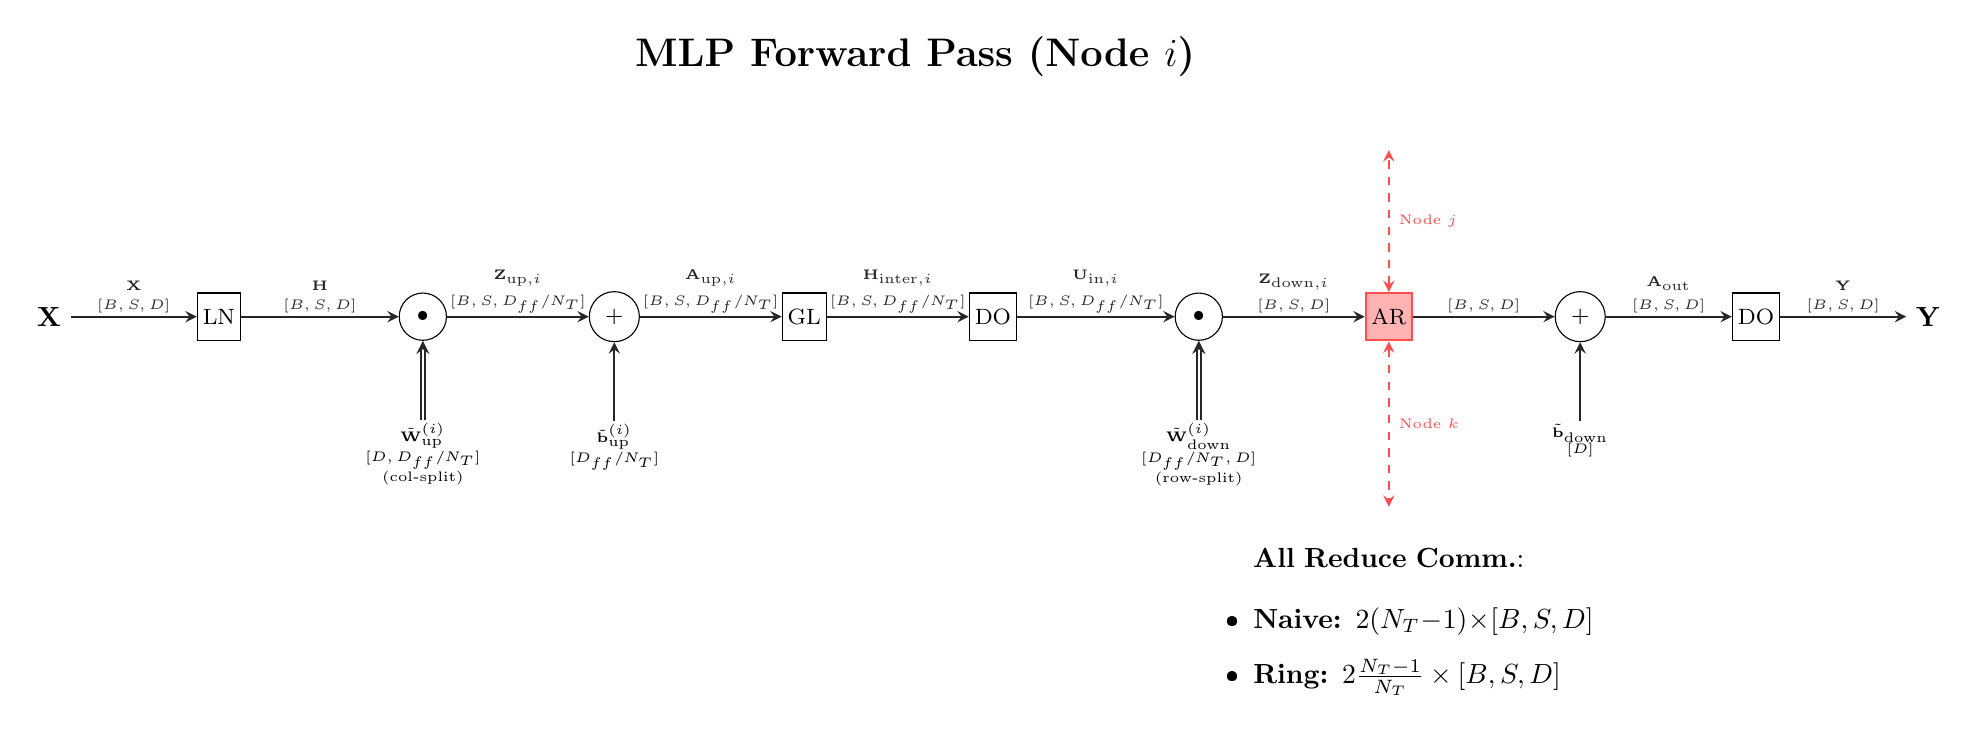
\begin{tikzpicture}[
    >=stealth,
    auxnode/.style={draw, rectangle, fill=white, minimum height=6mm, inner sep=2pt, font=\footnotesize, align=center},
    mulnode/.style={draw, circle, fill=white, minimum size=6mm, font=\footnotesize, align=center},
    addnode/.style={draw, circle, fill=white, minimum size=6mm, font=\footnotesize, align=center},
    allreduce/.style={draw, rectangle, fill=red!30, minimum height=6mm, inner sep=2pt, font=\footnotesize, align=center, thick, draw=red!70},
    sumnode/.style={draw, circle, fill=white, minimum size=6mm, font=\tiny, align=center},
    flow/.style={->, thick, black!85},
    flow2/.style={double, ->, thick, black!85},
    commflow/.style={<->, thick, red!70, dashed},
    dimlabel/.style={font=\tiny, inner sep=1pt, align=center}
]
    \node[font=\Large\bfseries] at (11, 2.8) {MLP Forward Pass (Node $i$)};

    \pgfmathsetmacro{\verticaloffset}{-0.5}

    \node            (MIn)   at (0,\verticaloffset) {$\mathbf{X}$};
    \node[auxnode]   (LN2)   [right=1.6cm of MIn] {LN};
    \node[mulnode]   (L1Mul) [right=2.0cm of LN2] {$\bullet$};
    \node[dimlabel]  (Wup)   [below=1.0cm of L1Mul] {$\tilde{\mathbf{W}}_{\text{up}}^{(i)}$\\$[D, D_{ff}/N_T]$\\(col-split)};
    \node[addnode]   (AddB1) [right=1.8cm of L1Mul] {+};
    \node[dimlabel]  (Bup)   [below=1.0cm of AddB1] {$\tilde{\mathbf{b}}_{\text{up}}^{(i)}$\\$[D_{ff}/N_T]$};
    \node[auxnode]   (Act)   [right=1.8cm of AddB1] {GL};
    \node[auxnode]   (Drop1) [right=1.8cm of Act] {DO};
    \node[mulnode]   (L2Mul) [right=2.0cm of Drop1] {$\bullet$};
    \node[dimlabel]  (Wdown) [below=1.0cm of L2Mul] {$\tilde{\mathbf{W}}_{\text{down}}^{(i)}$\\$[D_{ff}/N_T, D]$\\(row-split)};
    \node[allreduce] (AR)    [right=1.8cm of L2Mul] {AR};
    \node[
      align=center,
      below=2.5cm of AR,
      text width=5.2cm
    ] (AR_info) {%
      \textbf{All Reduce Comm.}:\\[2pt]
      \begin{itemize}
        \item \textbf{Naive:} $2(N_T-1) \times [B,S,D]$
        \item \textbf{Ring:} $2\frac{N_T-1}{N_T} \times [B,S,D]$
      \end{itemize}
    };
    \node[addnode]   (AddB2) [right=1.8cm of AR] {+};
    \node[dimlabel]  (Bdown) [below=1.0cm of AddB2] {$\tilde{\mathbf{b}}_{\text{down}}$\\$[D]$};
    \node[auxnode]   (Drop2) [right=1.6cm of AddB2] {DO};
    \node            (MOut)  [right=1.6cm of Drop2] {$\mathbf{Y}$};

    % All-Reduce communication arrows
    \draw[commflow] (AR.north) -- ++(0, 1.8) node[midway, right, font=\tiny]{Node $j$};
    \draw[commflow] (AR.south) -- ++(0, -2.1) node[midway, right, font=\tiny]{Node $k$};

    \draw[flow] (MIn) -- (LN2) node[dimlabel, midway, above]{\shortstack{$\mathbf{X}$\\$[B,S,D]$}};
    \draw[flow] (LN2) -- (L1Mul) node[dimlabel, midway, above]{\shortstack{$\mathbf{H}$\\$[B,S,D]$}};
    \draw[flow2] (Wup) -- (L1Mul);
    \draw[flow] (L1Mul) -- (AddB1) node[dimlabel, midway, above]{\shortstack{$\mathbf{Z}_{\text{up},i}$\\$[B,S,D_{ff}/N_T]$}};
    \draw[flow] (Bup) -- (AddB1);
    \draw[flow] (AddB1) -- (Act) node[dimlabel, midway, above]{\shortstack{$\mathbf{A}_{\text{up},i}$\\$[B,S,D_{ff}/N_T]$}};
    \draw[flow] (Act) -- (Drop1) node[dimlabel, midway, above]{\shortstack{$\mathbf{H}_{\text{inter},i}$\\$[B,S,D_{ff}/N_T]$}};
    \draw[flow] (Drop1) -- (L2Mul) node[dimlabel, midway, above]{\shortstack{$\mathbf{U}_{\text{in},i}$\\$[B,S,D_{ff}/N_T]$}};
    \draw[flow2] (Wdown) -- (L2Mul);
    \draw[flow] (L2Mul) -- (AR) node[dimlabel, midway, above]{\shortstack{$\mathbf{Z}_{\text{down},i}$\\$[B,S,D]$}};
    \draw[flow] (AR) -- (AddB2) node[dimlabel, midway, above]{\shortstack{$[B,S,D]$}};
    \draw[flow] (Bdown) -- (AddB2);
    \draw[flow] (AddB2) -- (Drop2) node[dimlabel, midway, above]{\shortstack{$\mathbf{A}_{\text{out}}$\\$[B,S,D]$}};
    \draw[flow] (Drop2) -- (MOut) node[dimlabel, midway, above]{\shortstack{$\mathbf{Y}$\\$[B,S,D]$}};

\end{tikzpicture}%
}
  \caption{텐서 병렬화된 MLP의 순전파.
  상향 프로젝션은 컬럼 병렬 선형으로 구현되어,
  각 디바이스가 중간 피처의 일부만을 보유한다.
  하향 프로젝션은 로우 병렬로 구현되며,
  디바이스 간 All-Reduce를 통해 전체
  $\mathbf{Z}_{\text{down}}$를 복원한 뒤,
  드롭아웃과 잔차 연결이 로컬로 적용된다.}
  \label{fig:mlp_forward_tp}
\end{figure}

\subsubsection{역전파}

텐서 병렬 MLP의 역전파는
단일 노드 역전파 그래프(Figure~\ref{fig:single_node_mlp_backward})와
동일한 구조를 사용하되,
파라미터와 활성값이 샤딩되어 있고,
적절한 위치에 All-Reduce가 들어간다는 점만 다르다.

각 디바이스에서 $\mathrm{d}\mathbf{Y}$로부터 시작하여
다음 순서로 진행된다.

\begin{enumerate}
  \item \textbf{잔차 및 드롭아웃 역전파}:
        단일 노드와 마찬가지로, 기울기는 항등 경로와
        최종 드롭아웃 경로로 나뉘어,
        각 디바이스에서 $\mathrm{d}\mathbf{Z}_{\text{down}}$을 얻는다.
  \item \textbf{하향 프로젝션 역전파 (로우 병렬)}:
        각 디바이스는 자신의 shard $W_{\text{down}}^{(t)}$와
        로컬 활성값 $\mathbf{U}^{(t)}$를 사용해
        \[
          \mathrm{d}\mathbf{U}^{(t)},\quad
          \mathrm{d}W_{\text{down}}^{(t)},\quad
          \mathrm{d}\mathbf{b}_{\text{down}}^{(t)}
        \]
        를 계산한다.
        $\mathrm{d}\mathbf{U}^{(t)}$를 구하는 데에는
        별도의 통신이 필요 없다.
  \item \textbf{활성 함수 역전파}:
        비선형 함수 $\phi$의 역전파를 각 디바이스에서 원소별로 적용하여
        $\mathrm{d}\mathbf{Z}_{\text{up}}^{(t)}$를 얻는다.
  \item \textbf{상향 프로젝션 역전파 (컬럼 병렬)}:
        컬럼 병렬 상향 프로젝션에 대해,
        각 디바이스는 $W_{\text{up}}^{(t)}$에 대한 로컬 기울기와
        입력에 대한 부분 기울기 $\mathrm{d}\mathbf{H}^{(t)}$를 계산한다.
        $\mathbf{H}$는 모든 디바이스에 공유되므로,
        이들을 합산해야 한다:
        \[
          \mathrm{d}\mathbf{H}
            = \sum_{t=0}^{N_T-1} \mathrm{d}\mathbf{H}^{(t)},
        \]
        이는 $t$에 대한 All-Reduce로 구현된다.
  \item \textbf{레이어 정규화 역전파(있는 경우)}:
        MLP 앞에 레이어 정규화가 있는 pre-LN 구조라면,
        $\mathrm{d}\mathbf{H}$는 추가적인 레이어 정규화 역전파를
        거쳐 이전 블록으로 전달된다.
\end{enumerate}

이러한 역전파 과정은 Figure~\ref{fig:mlp_backward_tp}에
전체 계산 그래프로 정리되어 있으며,
입력 기울기 $\mathrm{d}\mathbf{H}$에 대한 All-Reduce 위치가
명확히 표시되어 있다.

\begin{figure}[htbp]
  \centering
  \resizebox{\linewidth}{!}{%
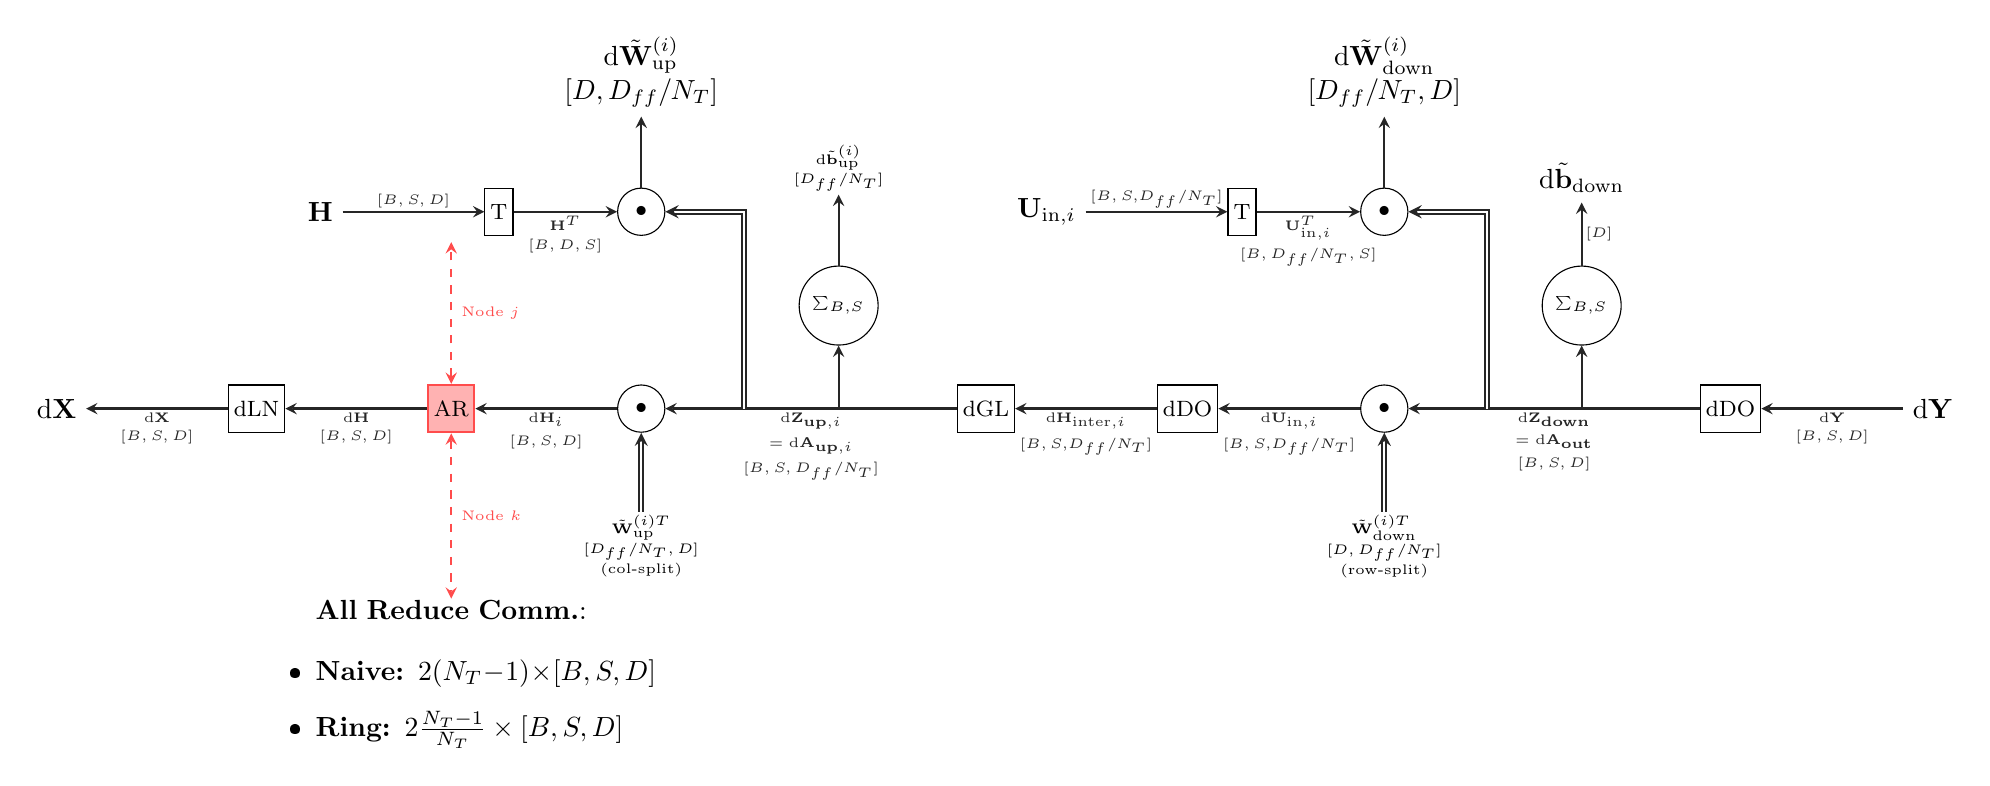
\begin{tikzpicture}[
    >=stealth,
    auxnode/.style={draw, rectangle, fill=white, minimum height=6mm, inner sep=2pt, font=\footnotesize, align=center},
    mulnode/.style={draw, circle, fill=white, minimum size=6mm, font=\footnotesize, align=center},
    addnode/.style={draw, circle, fill=white, minimum size=6mm, font=\footnotesize, align=center},
    sumnode/.style={draw, circle, fill=white, minimum size=6mm, font=\tiny, align=center},
    allreduce/.style={draw, rectangle, fill=red!30, minimum height=6mm, inner sep=2pt, font=\footnotesize, align=center, thick, draw=red!70},
    flow_rev/.style={<-, thick, black!85},
    flow_dw/.style={->, thick, black!85},
    flow_act/.style={double, ->, thick, black!85},
    commflow/.style={<->, thick, red!70, dashed},
    dimlabel/.style={font=\tiny, inner sep=1pt, align=center},
    gradlabel/.style={font=\tiny\bfseries, inner sep=1pt, align=center}
]
    % \node[font=\Large\bfseries] at (5, 10) {MLP Backward Pass (Node $i$)};

    \pgfmathsetmacro{\backwardoffset}{0.0}

    \node (d_MOut) at (12.6, \backwardoffset) {$\mathrm{d}\mathbf{Y}$};
    \node[auxnode] (d_Drop2) [left=1.8cm of d_MOut] {dDO};
    \draw[flow_rev] (d_Drop2) -- (d_MOut)
      node[dimlabel, midway, below]{\shortstack{$\mathrm{d}\mathbf{Y}$\\$[B,S,D]$}};

    \coordinate (split2) at ($(d_Drop2.west) + (-1.5cm, 0)$);
    \coordinate (branch_dUproj) at ($(split2) + (-1.2cm, 0)$);

    \node[sumnode] (d_SumB2) [above=0.8cm of split2] {$\sum_{B, S}$};
    \node (d_Bdown) [above=0.8cm of d_SumB2] {$\mathrm{d}\tilde{\mathbf{b}}_{\text{down}}$};
    \draw[flow_dw] (d_SumB2) -- (d_Bdown) node[dimlabel, midway, right]{$[D]$};

    \draw[flow_rev] (d_SumB2) -- (split2);

    \node[mulnode] (d_L2Mul_in) [left=2.2cm of split2] {$\bullet$};
    \draw[flow_rev] (d_L2Mul_in) -- (d_Drop2)
      node[gradlabel, midway, below]{\shortstack{$\mathrm{d}\mathbf{Z}_{\text{down}}$\\$=\mathrm{d}\mathbf{A}_{\text{out}}$\\$[B,S,D]$}};

    \node[dimlabel] (W_down_T) [align=center, below=1.0cm of d_L2Mul_in] {$\tilde{\mathbf{W}}_{\text{down}}^{(i)T}$\\$[D, D_{ff}/N_T]$\\(row-split)};
    \draw[flow_act] (W_down_T.north) -- (d_L2Mul_in);

    \coordinate (L2Mul_w_y) at ($(d_L2Mul_in) + (0, 2.5cm)$);
    \node[mulnode] (d_L2Mul_w) at (L2Mul_w_y) {$\bullet$};
    \node (d_Wdown) [align=center, above=0.9cm of d_L2Mul_w] {$\mathrm{d}\tilde{\mathbf{W}}_{\text{down}}^{(i)}$\\$[D_{ff}/N_T, D]$};
    \draw[flow_dw] (d_L2Mul_w) -- (d_Wdown);

    \draw[flow_act] (branch_dUproj.north) |- (d_L2Mul_w.east);

    \node[auxnode] (Uin_T) at ($(d_L2Mul_w.west) + (-1.5cm, 0)$) {T};
    \draw[flow_dw] (Uin_T) -- (d_L2Mul_w)
      node[dimlabel, midway, below]{\shortstack{$\mathbf{U}_{\text{in},i}^T$\\$[B, D_{ff}/N_T, S]$}};
    \node (Uin_aux) [left=1.8cm of Uin_T] {$\mathbf{U}_{\text{in},i}$};
    \draw[flow_dw] (Uin_aux) -- (Uin_T) node[dimlabel, midway, above]{\shortstack{$[B,S,$$D_{ff}/N_T]$}};

    \node[auxnode] (d_Drop1) [left=1.8cm of d_L2Mul_in] {dDO};
    \draw[flow_rev] (d_Drop1) -- (d_L2Mul_in)
      node[dimlabel, midway, below]{\shortstack{$\mathrm{d}\mathbf{U}_{\text{in},i}$\\$[B,S,$$D_{ff}/N_T]$}};

    \node[auxnode] (d_Act) [left=1.8cm of d_Drop1] {dGL};
    \draw[flow_rev] (d_Act) -- (d_Drop1)
      node[dimlabel, midway, below]{\shortstack{$\mathrm{d}\mathbf{H}_{\text{inter},i}$\\$[B,S,$$D_{ff}/N_T]$}};

    \coordinate (split1) at ($(d_Act.west) + (-1.5cm, 0)$);
    \coordinate (branch_dHpre) at ($(split1) + (-1.2cm, 0)$);

    \node[sumnode] (d_SumB1) [above=0.8cm of split1] {$\sum_{B, S}$};
    \node[dimlabel] (d_Bup) [above=0.9cm of d_SumB1] {$\mathrm{d}\tilde{\mathbf{b}}_{\text{up}}^{(i)}$\\$[D_{ff}/N_T]$};
    \draw[flow_dw] (d_SumB1) -- (d_Bup);

    \draw[flow_rev] (d_SumB1) -- (split1);

    \node[mulnode] (d_L1Mul_in) [left=2.2cm of split1] {$\bullet$};
    \draw[flow_rev] (d_L1Mul_in) -- (d_Act)
      node[gradlabel, midway, below]{\shortstack{$\mathrm{d}\mathbf{Z}_{\text{up},i}$\\$=\mathrm{d}\mathbf{A}_{\text{up},i}$\\$[B,S,D_{ff}/N_T]$}};

    \node[dimlabel] (W_up_T) [align=center, below=1.0cm of d_L1Mul_in] {$\tilde{\mathbf{W}}_{\text{up}}^{(i)T}$\\$[D_{ff}/N_T, D]$\\(col-split)};
    \draw[flow_act] (W_up_T.north) -- (d_L1Mul_in);

    \coordinate (L1Mul_w_y) at ($(d_L1Mul_in) + (0, 2.5cm)$);
    \node[mulnode] (d_L1Mul_w) at (L1Mul_w_y) {$\bullet$};
    \node (d_Wup) [align=center, above=0.9cm of d_L1Mul_w] {$\mathrm{d}\tilde{\mathbf{W}}_{\text{up}}^{(i)}$\\$[D, D_{ff}/N_T]$};
    \draw[flow_dw] (d_L1Mul_w) -- (d_Wup);

    \draw[flow_act] (branch_dHpre.north) |- (d_L1Mul_w.east);

    \node[auxnode] (Znorm_T) at ($(d_L1Mul_w.west) + (-1.5cm, 0)$) {T};
    \draw[flow_dw] (Znorm_T) -- (d_L1Mul_w)
      node[dimlabel, midway, below]{\shortstack{$\mathbf{H}^T$\\$[B, D, S]$}};
    \node (Znorm_aux) [left=1.8cm of Znorm_T] {$\mathbf{H}$};
    \draw[flow_dw] (Znorm_aux) -- (Znorm_T) node[dimlabel, midway, above]{\shortstack{$[B,S,D]$}};

    \node[allreduce] (AR) [left=1.8cm of d_L1Mul_in] {AR};
    \node[
      align=center,
      below=2.0cm of AR,
      text width=5.2cm
    ] (AR_info) {%
      \textbf{All Reduce Comm.}:\\[2pt]
      \begin{itemize}
        \item \textbf{Naive:} $2(N_T-1) \times [B,S,D]$
        \item \textbf{Ring:} $2\frac{N_T-1}{N_T} \times [B,S,D]$
      \end{itemize}
    };

    % All-Reduce communication arrows
    \draw[commflow] (AR.north) -- ++(0, 1.8) node[midway, right, font=\tiny]{Node $j$};
    \draw[commflow] (AR.south) -- ++(0, -2.1) node[midway, right, font=\tiny]{Node $k$};

    \draw[flow_rev] (AR) -- (d_L1Mul_in)
      node[dimlabel, midway, below]{\shortstack{$\mathrm{d}\mathbf{H}_i$\\$[B,S,D]$}};

    \node[auxnode] (d_LN2) [left=1.8cm of AR] {dLN};
    \draw[flow_rev] (d_LN2) -- (AR)
      node[dimlabel, midway, below]{\shortstack{$\mathrm{d}\mathbf{H}$\\$[B,S,D]$}};

    \node (d_MIn) [left=1.8cm of d_LN2] {$\mathrm{d}\mathbf{X}$};
    \draw[flow_rev] (d_MIn) -- (d_LN2)
      node[dimlabel, midway, below]{\shortstack{$\mathrm{d}\mathbf{X}$\\$[B,S,D]$}};
\end{tikzpicture}%
}
  \caption{텐서 병렬화된 MLP의 역전파.
  로우 병렬 down-projection, 활성 함수, 컬럼 병렬 up-projection,
  (필요 시) 레이어 정규화를 역순으로 따라가며,
  각 shard 파라미터와 입력에 대한 기울기를 계산한다.
  특히 up-projection에서 얻은 입력 기울기
  $\mathrm{d}\mathbf{H}^{(t)}$는 All-Reduce를 통해 합산되어
  전역 $\mathrm{d}\mathbf{H}$를 형성한다.}
  \label{fig:mlp_backward_tp}
\end{figure}

\subsection{요약}

요약하면, 텐서 병렬화는 단일 노드 트랜스포머의 각 큰 선형 연산을
컬럼 병렬 / 로우 병렬 패턴으로 구현함으로써,
\begin{itemize}
  \item 디바이스당 파라미터·활성값 메모리를 줄이고,
  \item 각 디바이스에서의 로컬 계산 구조는 단일 노드와 거의 동일하게 유지하며,
  \item 필요한 최소한의 All-Reduce / All-Gather를 통해
        단일 노드와 동일한 결과를 얻는다.
\end{itemize}

모든 경우에, 각 디바이스에서의 로컬 계산 그래프는
Section~\ref{sec:sn}에서 설명한 단일 노드 계산과 구조적으로 동일하다.
달라지는 것은 \emph{파라미터와 활성값을 어떻게 샤딩하는지, 그리고
어디에서 집합 통신을 수행하는지}뿐이다.
이 때문에 텐서 병렬화는 단일 노드 트랜스포머를 자연스럽게 확장한 형태로,
단일 가속기의 메모리에 들어가지 않는 대규모 모델에 특히 적합하다.

\else
  % ==========================================================
% 6. Tensor Parallelism (TP)
% ==========================================================
\section{Tensor Parallelism (TP)}
\label{sec:tp}

In tensor parallelism, the parameters of each layer are partitioned across
multiple devices along one or more tensor dimensions. Instead of
replicating the full weight matrix on every device, each device holds only
a shard of the weights and computes on a corresponding shard of the
activations. Collective communication (e.g., All-Reduce, All-Gather) is
then used to assemble partial results into the same shapes as in the
single-node model of Section~\ref{sec:sn}.

We denote the tensor-parallel degree by $N_T$, and index devices by
$t \in \{0,\dots,N_T-1\}$. Throughout this section we focus on how the
single-node computations from Section~\ref{sec:sn} are decomposed across these
$N_T$ devices.

\textbf{Key ideas.}
\begin{itemize}
  \item Large weight matrices are split along rows or columns so that each
        device holds a sub-matrix $W^{(t)}$ instead of the full matrix $W$.
  \item Each device computes local partial outputs using its own shard.
  \item Collective operations (All-Reduce, All-Gather) combine local
        partial results across devices into the same tensors that appear
        in the single-node computation graph.
  \item The backward pass mirrors the sharding and communication pattern
        of the forward pass so that gradients with respect to parameters
        and inputs are correctly accumulated.
  \item Memory usage per device is reduced approximately by a factor of
        $N_T$, but each global matmul incurs at least one collective
        communication.
\end{itemize}

\subsection{Overview of Tensor-Parallel Sharding}

At a high level, tensor parallelism can be seen as replacing every large
matrix multiplication in Section~\ref{sec:sn} with a collection of smaller matmuls
that run in parallel on different devices. There are two basic patterns
for sharding a linear layer
\[
  \mathbf{Y} = \mathbf{X} W + \mathbf{b}, \qquad
  \mathbf{X} \in \mathbb{R}^{B \times D_{\text{in}}},\;
  W \in \mathbb{R}^{D_{\text{in}} \times D_{\text{out}}}:
\]
\begin{itemize}
  \item \textbf{Column-parallel (output-sharded) linear}: split $W$ along
        the output dimension,
        $W = [W^{(0)},\dots,W^{(N_T-1)}]$ with
        $W^{(t)} \in \mathbb{R}^{D_{\text{in}} \times D_{\text{out}}^{(t)}}$.
        Each device computes
        $\mathbf{Y}^{(t)} = \mathbf{X} W^{(t)} + \mathbf{b}^{(t)}$, and
        the global output is obtained by concatenation:
        \[
          \mathbf{Y} = \mathrm{Concat}_t \mathbf{Y}^{(t)}.
        \]
        No collective is needed on the forward path, but later layers may
        require an All-Gather or All-Reduce to reassemble or sum over
        shards.
  \item \textbf{Row-parallel (input-sharded) linear}: split $W$ along the
        input dimension and shard $\mathbf{X}$ accordingly. Each device
        holds $X^{(t)}$ and $W^{(t)}$ with
        $W^{(t)} \in \mathbb{R}^{D_{\text{in}}^{(t)} \times D_{\text{out}}}$,
        computes a partial product
        $\mathbf{Y}^{(t)} = \mathbf{X}^{(t)} W^{(t)}$, and an All-Reduce
        across $t$ produces the full output:
        \[
          \mathbf{Y} = \sum_{t=0}^{N_T-1} \mathbf{Y}^{(t)}.
        \]
\end{itemize}

These two patterns are composed inside the Transformer so that most
operations remain local to each device and only a small number of
All-Reduce/All-Gather calls are required per layer. An overview of this
scheme for a single Transformer block is shown in
Figure~\ref{fig:tp_overall_flow}, which should be compared to the
single-node overview in Figure~\ref{fig:single_node_overall}.

\begin{figure}[htbp]
  \centering
  \resizebox{\linewidth}{!}{%
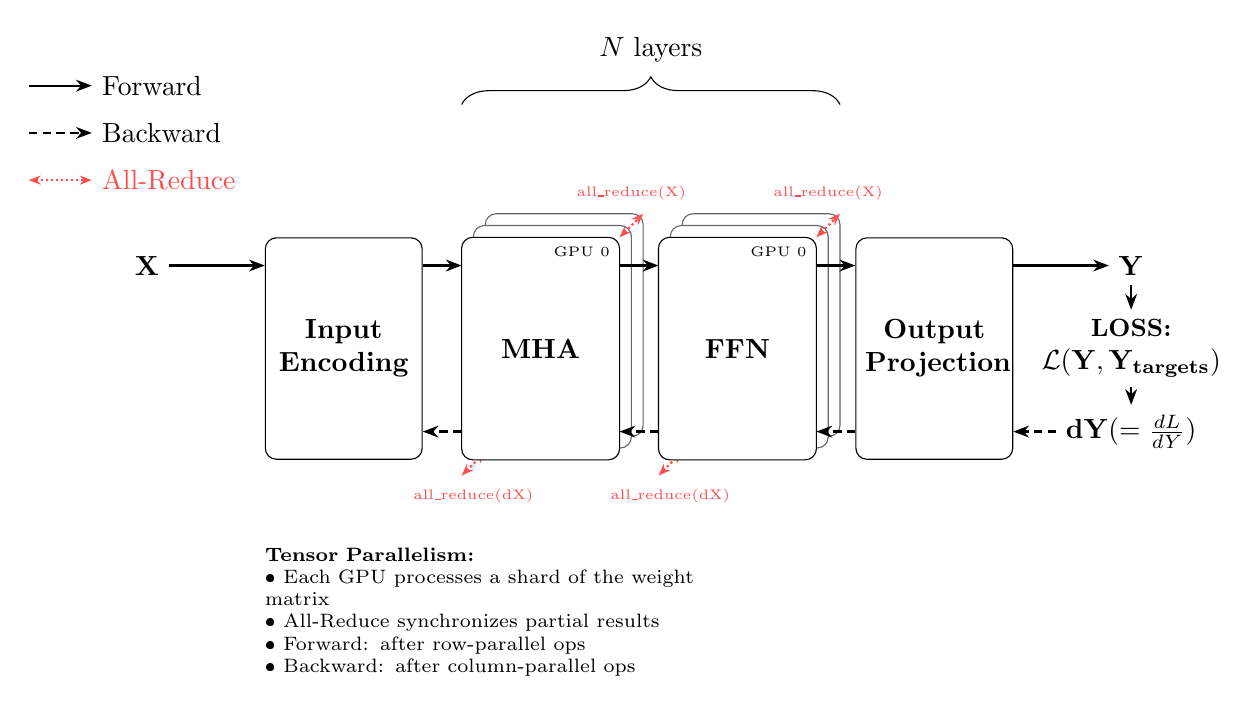
\begin{tikzpicture}[
    node distance=2.5cm,
    >=stealth,
    block/.style={rectangle, draw=black, fill=white, text width=5em, text centered, rounded corners, minimum height=8em, font=\bfseries},
    blockstack/.style={rectangle, draw=black!60, fill=white, text width=5em, text centered, rounded corners, minimum height=8em},
    forward/.style={-{Stealth[length=2mm]}, thick, black},
    backward/.style={-{Stealth[length=2mm]}, thick, black, densely dashed},
    allreduce/.style={{Stealth[length=1.5mm]}-{Stealth[length=1.5mm]}, thick, red!70, densely dotted},
    io/.style={text centered, font=\bfseries}
]
    % Title
    % \node[font=\Large\bfseries] at (10, 6) {Transformer Overall Flow (TP with 3 GPUs)};

    % Forward path nodes (horizontal)
    \node (input) [io] {$\mathbf{X}$};
    \node (encoding) [block, right of=input, yshift=-3em] {Input\\Encoding};

    % MHA blocks (3 stacked) - GPU 2 (back)
    \node (mha3) [blockstack, right of=encoding, xshift=0.3cm, yshift=0.3cm] {};
    % MHA blocks (3 stacked) - GPU 1 (middle)
    \node (mha2) [blockstack, right of=encoding, xshift=0.15cm, yshift=0.15cm] {};
    % MHA blocks (3 stacked) - GPU 0 (front)
    \node (mha) [block, right of=encoding] {MHA};

    % Small GPU labels for MHA
    \node[font=\tiny, anchor=north east] at (mha.north east) {GPU 0};

    % FFN blocks (3 stacked) - GPU 2 (back)
    \node (mlp3) [blockstack, right of=mha, xshift=0.3cm, yshift=0.3cm] {};
    % FFN blocks (3 stacked) - GPU 1 (middle)
    \node (mlp2) [blockstack, right of=mha, xshift=0.15cm, yshift=0.15cm] {};
    % FFN blocks (3 stacked) - GPU 0 (front)
    \node (mlp) [block, right of=mha] {FFN};

    % Small GPU labels for FFN
    \node[font=\tiny, anchor=north east] at (mlp.north east) {GPU 0};

    \node (output) [block, right of=mlp] {Output\\Projection};
    \node (pred) [io, right of=output, yshift=3em] {$\mathbf{Y}$};
    \node (loss) [align=center, io, right of=output] {\small LOSS:\\$\mathcal{L}(\mathbf{Y,Y_\text{targets}})$};
    \node (gradient) [io, right of=output, yshift=-3em] {$\mathbf{dY}(=\frac{dL}{dY})$};

    % All-Reduce arrows (Backward drawn first, then blocks, then Forward on top)
    % Backward All-Reduce - FFN (left-bottom corner, lower position)
    \draw [allreduce] ([yshift=-0.2cm]mlp.south west) -- ([xshift=0.3cm, yshift=0.1cm]mlp.south west);
    \node[font=\tiny, red!70, anchor=north] at ([xshift=0.15cm, yshift=-0.25cm]mlp.south west) {all\_reduce(dX)};

    % Backward All-Reduce - MHA (left-bottom corner, lower position)
    \draw [allreduce] ([yshift=-0.2cm]mha.south west) -- ([xshift=0.3cm, yshift=0.1cm]mha.south west);
    \node[font=\tiny, red!70, anchor=north] at ([xshift=0.15cm, yshift=-0.25cm]mha.south west) {all\_reduce(dX)};

    % Redraw blocks to cover backward All-Reduce arrows
    \draw [draw=black!60, fill=white, rounded corners] (mha3.south west) rectangle (mha3.north east);
    \draw [draw=black!60, fill=white, rounded corners] (mha2.south west) rectangle (mha2.north east);
    \draw [draw=black, fill=white, rounded corners, line width=0.4pt] (mha.south west) rectangle (mha.north east);
    \node[font=\bfseries] at (mha.center) {MHA};
    \node[font=\tiny, anchor=north east] at (mha.north east) {GPU 0};

    \draw [draw=black!60, fill=white, rounded corners] (mlp3.south west) rectangle (mlp3.north east);
    \draw [draw=black!60, fill=white, rounded corners] (mlp2.south west) rectangle (mlp2.north east);
    \draw [draw=black, fill=white, rounded corners, line width=0.4pt] (mlp.south west) rectangle (mlp.north east);
    \node[font=\bfseries] at (mlp.center) {FFN};
    \node[font=\tiny, anchor=north east] at (mlp.north east) {GPU 0};

    % Forward All-Reduce - MHA (right-top corner) - drawn after blocks to appear on top
    \draw [allreduce] (mha.north east) -- ([xshift=0.3cm, yshift=0.3cm]mha.north east);
    \node[font=\tiny, red!70, anchor=south] at ([xshift=0.15cm, yshift=0.35cm]mha.north east) {all\_reduce(X)};

    % Forward All-Reduce - FFN (right-top corner) - drawn after blocks to appear on top
    \draw [allreduce] (mlp.north east) -- ([xshift=0.3cm, yshift=0.3cm]mlp.north east);
    \node[font=\tiny, red!70, anchor=south] at ([xshift=0.15cm, yshift=0.35cm]mlp.north east) {all\_reduce(X)};

    % Forward arrows (upper part of blocks)
    \draw [forward] (input) -- ([yshift=3em]encoding.west);
    \draw [forward] ([yshift=3em]encoding.east) -- ([yshift=3em]mha.west);
    \draw [forward] ([yshift=3em]mha.east) -- ([yshift=3em]mlp.west);
    \draw [forward] ([yshift=3em]mlp.east) -- ([yshift=3em]output.west);
    \draw [forward] ([yshift=3em]output.east) -- (pred);
    \draw [forward] (pred) -- (loss);
    \draw [backward] (loss) -- (gradient);

    % Backward arrows (lower part of blocks)
    \draw [backward] (gradient) -- ([yshift=-3em]output.east);
    \draw [backward] ([yshift=-3em]output.west) -- ([yshift=-3em]mlp.east);
    \draw [backward] ([yshift=-3em]mlp.west) -- ([yshift=-3em]mha.east);
    \draw [backward] ([yshift=-3em]mha.west) -- ([yshift=-3em]encoding.east);

    % Brace for layer repetition (horizontal - using mlp with x offset to match mlp3)
    \draw[decorate, decoration={brace, amplitude=10pt}]
        ([yshift=4.8em]mha.north west) -- ([xshift=0.3cm, yshift=4.8em]mlp.north east)
        node[midway, above=12pt, font=\normalsize] {$N$ layers};

    % Labels (Legend)
    \coordinate (legend) at ([xshift=-1.5cm, yshift=6.5em]input);
    \draw[forward] (legend) -- ++(0.8,0) node[right, font=\normalsize] {Forward};
    \draw[backward] ([yshift=-0.6cm]legend) -- ++(0.8,0) node[right, font=\normalsize] {Backward};
    \draw[allreduce] ([yshift=-1.2cm]legend) -- ++(0.8,0) node[right, font=\normalsize] {All-Reduce};

    % TP explanation
    \node[font=\scriptsize, align=left, text width=6cm] at ([xshift=2cm, yshift=-5.5em]encoding.south) {
        \textbf{Tensor Parallelism:}\\
        • Each GPU processes a shard of the weight matrix\\
        • All-Reduce synchronizes partial results\\
        • Forward: after row-parallel ops\\
        • Backward: after column-parallel ops
    };

\end{tikzpicture}%
}
  \caption{Overall Transformer layer with tensor parallelism. Each large
  linear layer from the single-node model is replaced by $N_T$ smaller
  matmuls on different devices. Colored arrows indicate where collective
  communication (e.g.\ All-Reduce, All-Gather) is required to assemble
  partial results, while local computations remain identical to those in
  Figure~\ref{fig:single_node_overall}.}
  \label{fig:tp_overall_flow}
\end{figure}

% ------------------------ 6.1 MHA with Tensor Parallelism -------------
\subsection{MHA with Tensor Parallelism}

We now apply tensor parallelism to the multi-head attention (MHA) block.
Recall from Section~\ref{sec:sn}.2 that the single-node attention block maps
$\mathbf{X} \in [B,S,D]$ to
$\mathbf{A}_{\text{out}} \in [B,S,D]$ via Q/K/V projections, scaled dot
product attention, an output projection, and a residual connection.

In tensor parallelism we partition these computations across $N_T$
devices in such a way that:
\begin{itemize}
  \item each device is responsible for a subset of the attention heads, or
        equivalently a subset of the output channels of the Q/K/V
        projections;
  \item the softmax and value-weighted sums are computed locally on each
        device for its own heads;
  \item the final output projection is implemented as a row-parallel
        linear, requiring an All-Reduce across devices to recover the
        same $\mathbf{A}_{\text{out}}$ as in the single-node case.
\end{itemize}

Figure~\ref{fig:mha_forward_tp} shows the forward data flow under this
sharding scheme and should be read as a “TP-annotated” version of
Figure~\ref{fig:single_node_mha_forward}. The corresponding backward
graph is shown in Figure~\ref{fig:mha_backward_tp}.

\subsubsection{Forward Pass}

For clarity we focus on one Transformer block and omit batch/sequence
dimensions in some formulas. We write the per-device Q/K/V projections as
column-parallel linears:
\[
  W_Q = [W_Q^{(0)},\dots,W_Q^{(N_T-1)}],\quad
  W_K = [W_K^{(0)},\dots,W_K^{(N_T-1)}],\quad
  W_V = [W_V^{(0)},\dots,W_V^{(N_T-1)}],
\]
where, on device $t$,
\[
  W_Q^{(t)}, W_K^{(t)}, W_V^{(t)}
    \in \mathbb{R}^{D \times D_h^{(t)}}, \qquad
  \sum_t D_h^{(t)} = D.
\]
Each device computes local projections:
\[
  \mathbf{Q}^{(t)} = \mathbf{X}_{\text{norm}} W_Q^{(t)},\quad
  \mathbf{K}^{(t)} = \mathbf{X}_{\text{norm}} W_K^{(t)},\quad
  \mathbf{V}^{(t)} = \mathbf{X}_{\text{norm}} W_V^{(t)},
\]
and reshapes them into its own subset of attention heads. Because heads
are independent, each device can compute the scaled dot-product attention
for its local heads without communication:
\[
  \mathbf{S}^{(t)} = \frac{\mathbf{Q}^{(t)} (\mathbf{K}^{(t)})^{\top}}
                           {\sqrt{D_h^{(t)}}},\qquad
  \mathbf{A}_S^{(t)} = \mathrm{Softmax}(\mathrm{Mask}(\mathbf{S}^{(t)})),
\]
\[
  \mathbf{A}_{\text{heads}}^{(t)} = \mathbf{A}_S^{(t)} \mathbf{V}^{(t)}.
\]

After computing local head outputs, each device forms a local
concatenation
$\mathbf{A}_{\text{cat}}^{(t)} \in \mathbb{R}^{B \times S \times D^{(t)}}$
over its subset of heads. The final output projection is implemented as a
\emph{row-parallel} linear:
\[
  W_O = \begin{bmatrix} W_O^{(0)} \\ \vdots \\ W_O^{(N_T-1)} \end{bmatrix},
  \quad W_O^{(t)} \in \mathbb{R}^{D^{(t)} \times D}.
\]
Each device computes a partial contribution
\[
  \mathbf{A}_{\text{lin}}^{(t)}
    = \mathbf{A}_{\text{cat}}^{(t)} W_O^{(t)} + \mathbf{b}_O^{(t)},
\]
and an All-Reduce across $t$ yields the full projected tensor
\[
  \mathbf{A}_{\text{lin}}
    = \sum_{t=0}^{N_T-1} \mathbf{A}_{\text{lin}}^{(t)}.
\]
Dropout and the residual connection with $\mathbf{X}$ are then applied
locally on each device, since after the All-Reduce every device holds the
same $\mathbf{A}_{\text{lin}}$ and $\mathbf{X}$.

These steps, together with the location of the All-Reduce, are annotated
explicitly in Figure~\ref{fig:mha_forward_tp}.

\begin{landscape}
\begin{figure}[p]
  \centering
  \resizebox{\linewidth}{!}{%
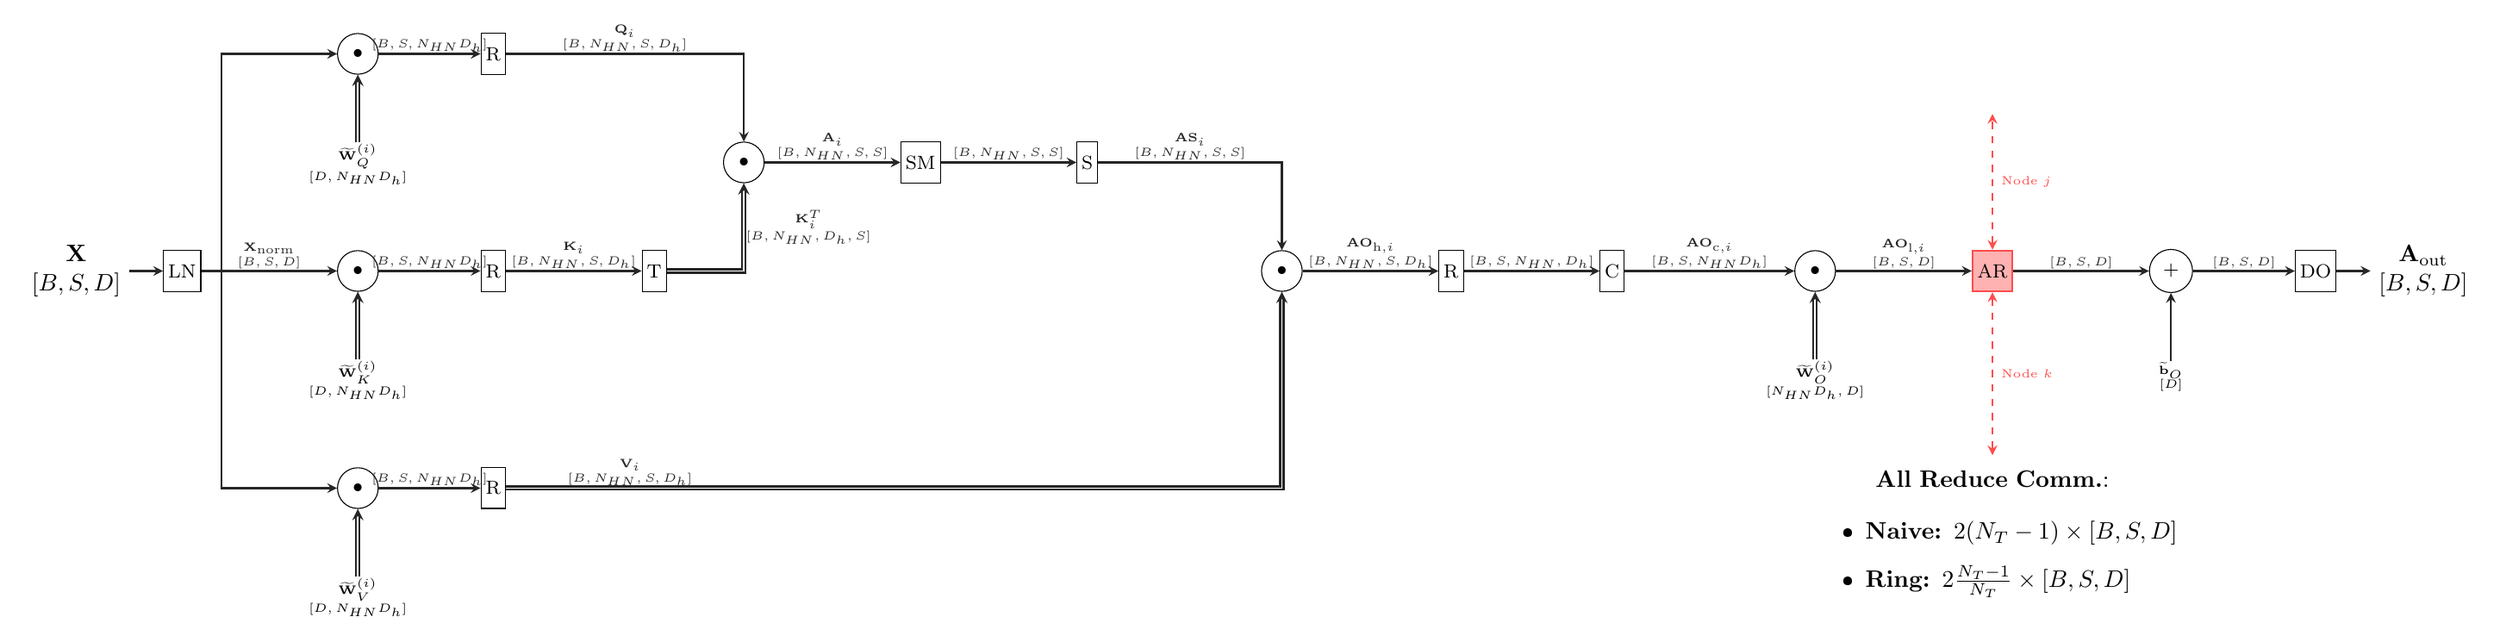
\begin{tikzpicture}[
  every node/.style={transform shape},
  >=stealth,
  auxnode/.style={draw, rectangle, fill=white, minimum height=6mm, inner sep=2pt, font=\footnotesize, align=center},
  mulnode/.style={draw, circle, fill=white, minimum size=6mm, font=\footnotesize, align=center},
  addnode/.style={draw, circle, fill=white, minimum size=6mm, font=\footnotesize, align=center},
  allreduce/.style={draw, rectangle, fill=red!30, minimum height=6mm, inner sep=2pt, font=\footnotesize, align=center, thick, draw=red!70},
  flow/.style={->, thick, black!85},
  flow2/.style={->, double, thick, black!85},
  commflow/.style={<->, thick, red!70, dashed},
  dimlabel/.style={font=\tiny, inner sep=0.5pt, align=center}
]
% \node[font=\Large\bfseries] at (9, 4.5) {Multi-Head Attention Forward Pass (Node $i$)};

\node (Input) at (0.5, 0) [align=center] {$\mathbf{X}$\\$[B,S,D]$};
\node[auxnode] (LN) [right=0.5cm of Input] {LN};

\node[mulnode] (Proj_Q) [right=2.0cm of LN, yshift=3.2cm] {$\bullet$};
\node[auxnode] (R_Q) [right=1.5cm of Proj_Q] {R};

\node[mulnode] (Proj_K) [right=2.0cm of LN, yshift=0cm] {$\bullet$};
\node[auxnode] (R_K) [right=1.5cm of Proj_K] {R};

\node[mulnode] (Proj_V) [right=2.0cm of LN, yshift=-3.2cm] {$\bullet$};
\node[auxnode] (R_V) [right=1.5cm of Proj_V] {R};

\node[dimlabel] (WQ) [align=center, below=1.0cm of Proj_Q] {$\widetilde{\mathbf{W}}_{Q}^{(i)}$\\$[D,N_{HN}D_h]$};
\node[dimlabel] (WK) [align=center, below=1.0cm of Proj_K] {$\widetilde{\mathbf{W}}_{K}^{(i)}$\\$[D,N_{HN}D_h]$};
\node[dimlabel] (WV) [align=center, below=1.0cm of Proj_V] {$\widetilde{\mathbf{W}}_{V}^{(i)}$\\$[D,N_{HN}D_h]$};

\node[auxnode] (T_K) [right=2.0cm of R_K] {T};
\node[mulnode] (QK) [right=3.2cm of R_Q, yshift=-1.6cm] {$\bullet$};
\node[auxnode] (SM) [right=2.0cm of QK] {SM};
\node[auxnode] (Soft) [right=2.0cm of SM] {S};
\node[mulnode] (PV) [right=2.4cm of Soft, yshift=-1.6cm] {$\bullet$};

\node[auxnode] (R_Merge) [right=2.0cm of PV] {R};
\node[auxnode] (Cat) [right=2.0cm of R_Merge] {C};

\node[mulnode] (OProj) [right=2.5cm of Cat] {$\bullet$};
\node[dimlabel] (WO_FWD) [align=center, below=1.0cm of OProj] {$\widetilde{\mathbf{W}}_{O}^{(i)}$\\$[N_{HN}D_h,D]$};
\node[allreduce] (AR) [right=2.0cm of OProj] {AR};
\node[
  align=center,
  below=2.5cm of AR,
  text width=5.5cm % 적당한 값으로 조정
] (AR_info) {%
  \textbf{All Reduce Comm.}:\\[2pt]
  \begin{itemize}
    \item \textbf{Naive:} $2(N_T-1) \times [B,S,D]$
    \item \textbf{Ring:} $2\frac{N_T-1}{N_T} \times [B,S,D]$
  \end{itemize}
};
\node[addnode] (AddB) [right=2.0cm of AR] {+};
\node[dimlabel] (BO) [align=center, below=1.0cm of AddB] {$\widetilde{\mathbf{b}}_{O}$\\$[D]$};
\node[auxnode] (Drop) [right=1.5cm of AddB] {DO};
\node (Aout) [align=center, right=0.5cm of Drop] {$\mathbf{A}_{\text{out}}$\\$[B,S,D]$};

\draw[flow] (Input) -- (LN);

\draw[flow] (LN.east) -- ++(0.3,0) |- (Proj_Q.west);
\draw[flow] (LN) -- (Proj_K.west) node[dimlabel, midway, above]{$\mathbf{X}_{\text{norm}}$\\$[B,S,D]$};
\draw[flow] (LN.east) -- ++(0.3,0) |- (Proj_V.west);

\draw[flow2] (WQ) -- (Proj_Q);
\draw[flow2] (WK) -- (Proj_K);
\draw[flow2] (WV) -- (Proj_V);

\draw[flow] (Proj_Q) -- (R_Q) node[dimlabel, midway, above]{$[B,S,N_{HN}D_h]$};
\draw[flow] (Proj_K) -- (R_K) node[dimlabel, midway, above]{$[B,S,N_{HN}D_h]$};
\draw[flow] (Proj_V) -- (R_V) node[dimlabel, midway, above]{$[B,S,N_{HN}D_h]$};

\draw[flow] (R_Q) -| (QK) node[dimlabel, near start, above]{$\mathbf{Q}_i$\\$[B,N_{HN},S,D_h]$};
\draw[flow] (R_K) -- (T_K) node[dimlabel, midway, above]{$\mathbf{K}_i$\\$[B,N_{HN},S,D_h]$};
\draw[flow2] (T_K) -| (QK) node[dimlabel, near end, right]{$\mathbf{K}_i^{T}$\\$[B,N_{HN},D_h,S]$};

\draw[flow] (QK) -- (SM) node[dimlabel, midway, above]{$\mathbf{A}_i$\\$[B,N_{HN},S,S]$};
\draw[flow] (SM) -- (Soft) node[dimlabel, midway, above]{$[B,N_{HN},S,S]$};
\draw[flow] (Soft) -| (PV) node[dimlabel, near start, above]{$\mathbf{AS}_i$\\$[B,N_{HN},S,S]$};
\draw[flow2] (R_V) -| (PV) node[dimlabel, pos=0.08, above]{$\mathbf{V}_i$\\$[B,N_{HN},S,D_h]$};

\draw[flow] (PV) -- (R_Merge) node[dimlabel, midway, above]{$\mathbf{AO}_{\text{h},i}$\\$[B,N_{HN},S,D_h]$};
\draw[flow] (R_Merge) -- (Cat) node[dimlabel, midway, above]{$[B,S,N_{HN},D_h]$};
\draw[flow] (Cat) -- (OProj) node[dimlabel, midway, above]{$\mathbf{AO}_{\text{c},i}$\\$[B,S,N_{HN}D_h]$};
\draw[flow2] (WO_FWD) -- (OProj);
\draw[flow] (OProj) -- (AR) node[dimlabel, midway, above]{$\mathbf{AO}_{\text{l},i}$\\$[B,S,D]$};

% All-Reduce communication arrows
\draw[commflow] (AR.north) -- ++(0, 2.0) node[midway, right, font=\tiny]{Node $j$};
\draw[commflow] (AR.south) -- ++(0, -2.4) node[midway, right, font=\tiny]{Node $k$};

\draw[flow] (AR) -- (AddB) node[dimlabel, midway, above]{$[B,S,D]$};
\draw[flow] (BO) -- (AddB);
\draw[flow] (AddB) -- (Drop) node[dimlabel, midway, above]{$[B,S,D]$};
\draw[flow] (Drop) -- (Aout);
\end{tikzpicture}%
}
  \caption{Multi-head attention forward pass with tensor parallelism. Q/K/V
  projections are implemented as column-parallel linears so that each
  device owns a subset of the heads. Attention for each local head is
  computed independently, and the resulting head outputs are combined
  using a row-parallel output projection followed by an All-Reduce to
  recover the same $\mathbf{A}_{\text{out}}$ as in the single-node
  computation.}
  \label{fig:mha_forward_tp}
\end{figure}
\end{landscape}

\subsubsection{Backward Pass}

The backward pass for tensor-parallel MHA follows the same high-level
structure as in Section~\ref{sec:sn}.2, but with sharded gradients and explicit
collectives. Starting from
$\mathrm{d}\mathbf{A}_{\text{out}}$ on each device, we have:

\begin{itemize}
  \item \textbf{Output projection backward.}
        The row-parallel output projection produces local gradients
        $\mathrm{d}\mathbf{A}_{\text{cat}}^{(t)}$ and parameter gradients
        $\mathrm{d}W_O^{(t)}, \mathrm{d}\mathbf{b}_O^{(t)}$ from
        $\mathrm{d}\mathbf{A}_{\text{lin}}$.
  \item \textbf{Head backward.}
        Each device backpropagates through its local heads, computing
        $\mathrm{d}\mathbf{V}^{(t)}$ and $\mathrm{d}\mathbf{A}_S^{(t)}$,
        and then $\mathrm{d}\mathbf{Q}^{(t)}$ and
        $\mathrm{d}\mathbf{K}^{(t)}$ through the scaled dot-product and
        softmax.
  \item \textbf{Q/K/V projection backward.}
        The column-parallel Q/K/V linears produce local gradients
        $\mathrm{d}W_Q^{(t)}, \mathrm{d}W_K^{(t)}, \mathrm{d}W_V^{(t)}$
        and partial contributions to the gradient w.r.t.\ the normalized
        input, $\mathrm{d}\mathbf{X}_{\text{norm}}^{(t)}$.
  \item \textbf{All-Reduce for input gradient.}
        Because $\mathbf{X}_{\text{norm}}$ is shared across devices,
        gradients from all Q/K/V shards must be summed:
        \[
          \mathrm{d}\mathbf{X}_{\text{norm}}
            = \sum_{t=0}^{N_T-1} \mathrm{d}\mathbf{X}_{\text{norm}}^{(t)},
        \]
        implemented as an All-Reduce over $t$.
  \item \textbf{Layer normalization backward.}
        Finally, layer normalization backward is applied locally on each
        device to produce $\mathrm{d}\mathbf{X}$ and gradients for the LN
        parameters, exactly as in the single-node setting.
\end{itemize}

Figure~\ref{fig:mha_backward_tp} expands these steps into a full
computation graph, with each All-Reduce/All-Gather explicitly indicated.

\begin{landscape}
\begin{figure}[p]
  % no \centering here to avoid compilation issues
  \par\vspace{1cm}
\noindent
\resizebox{\linewidth}{!}{%
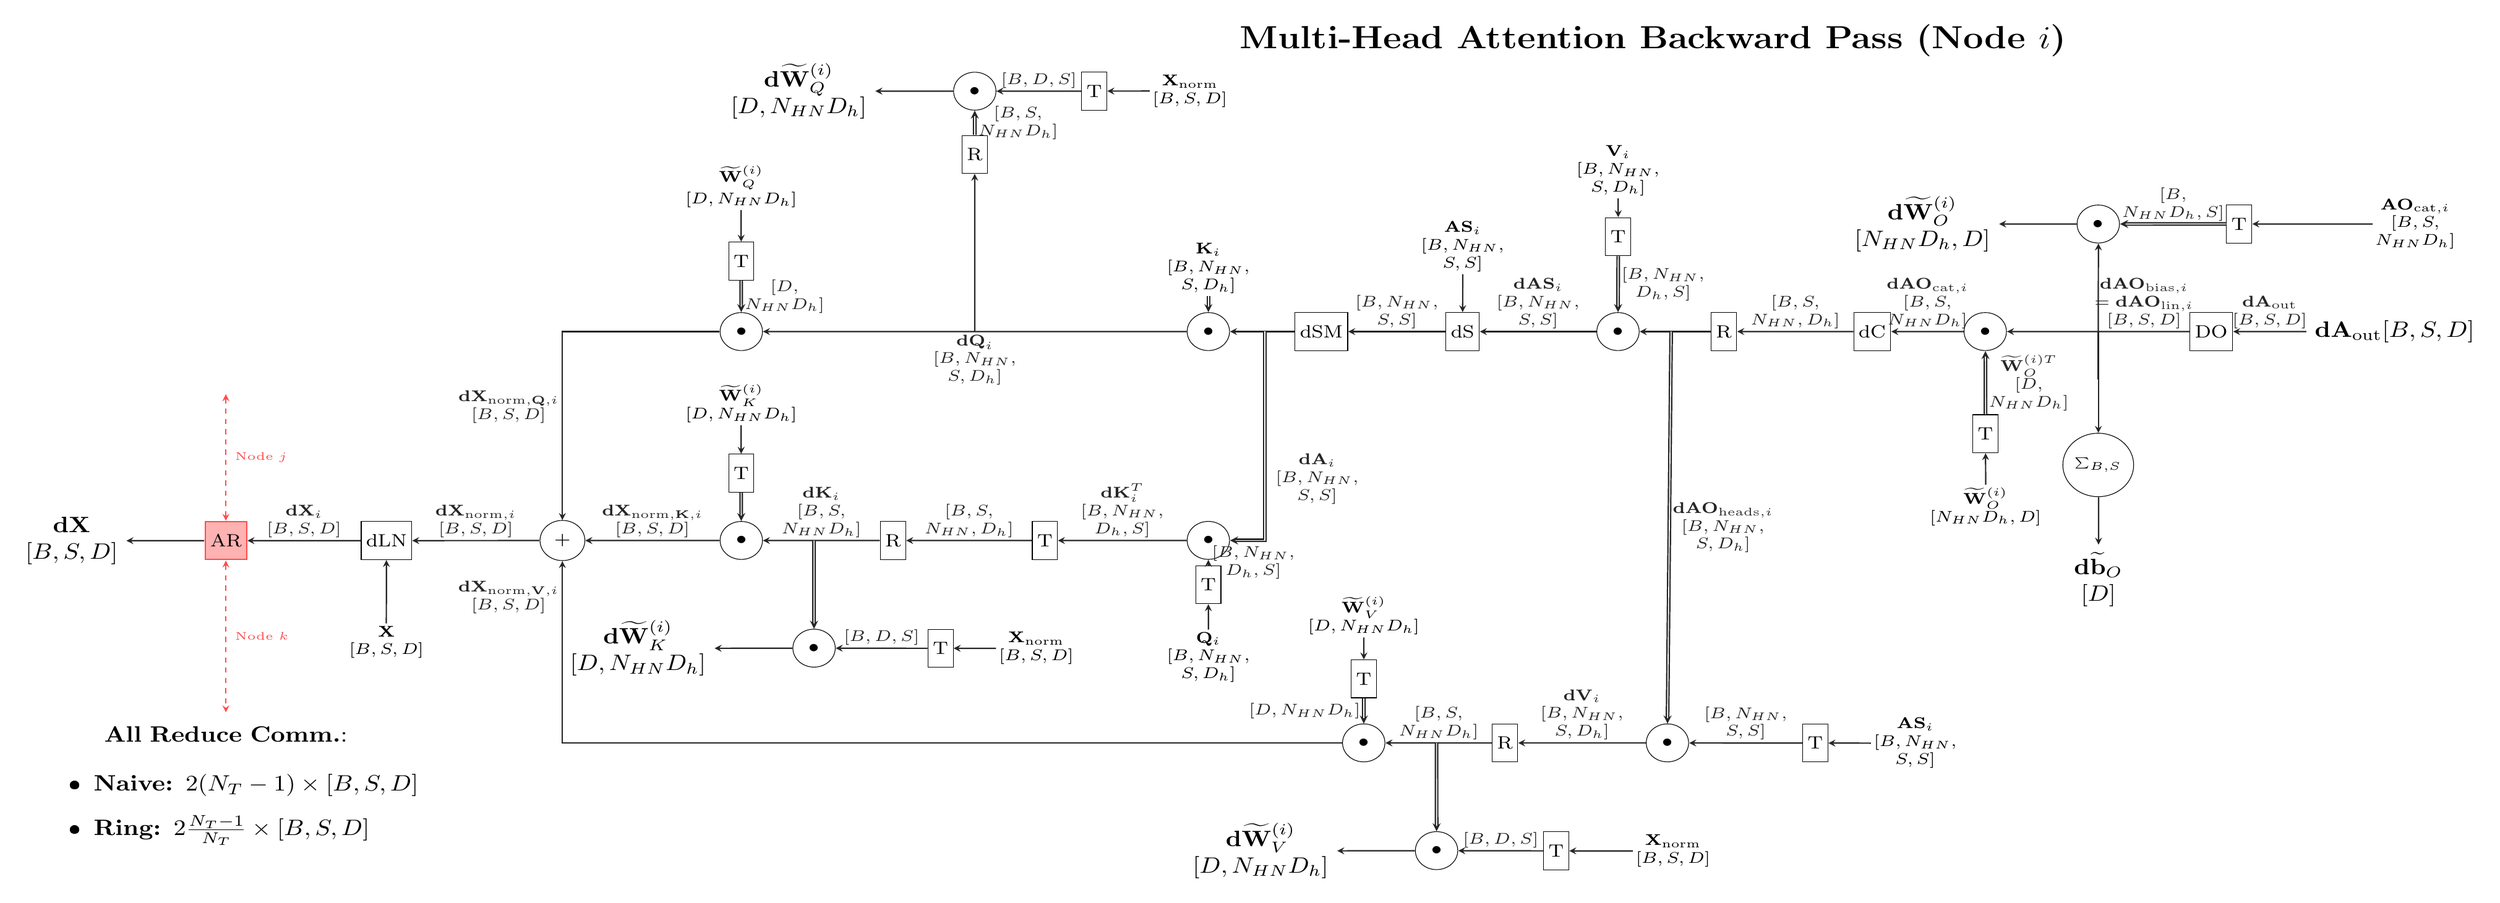
\begin{tikzpicture}[
  every node/.style={transform shape},
  >=stealth,
  auxnode/.style={draw, rectangle, fill=white, minimum height=6mm, inner sep=2pt, font=\footnotesize, align=center},
  mulnode/.style={draw, circle, fill=white, minimum size=6mm, font=\footnotesize, align=center},
  addnode/.style={draw, circle, fill=white, minimum size=6mm, font=\footnotesize, align=center},
  sumnode/.style={draw, circle, fill=white, minimum size=6mm, font=\tiny, align=center},
  allreduce/.style={draw, rectangle, fill=red!30, minimum height=6mm, inner sep=2pt, font=\footnotesize, align=center, thick, draw=red!70},
  flow/.style={->, thick, black!85},
  flow2/.style={->, double, thick, black!85},
  commflow/.style={<->, thick, red!70, dashed},
  dimlabel/.style={font=\scriptsize, inner sep=1pt, align=center},
  gradflow/.style={->, thick, black!85},
  gradweight/.style={->, thick, black!85}
]

\begin{scope}[xscale=1.45, yscale=1.3]

\def\yoffset{-1.0}
\def\dVXyoffset{-6.5}

\coordinate (Grad_Aout_B) at (17.5, \yoffset);
\coordinate (dDrop_center) at (15.9, \yoffset);
\coordinate (ProjGradSplit) at (14.3, \yoffset);
\coordinate (dOProj_center) at (12.7, \yoffset);
\coordinate (C_center) at (11.1, \yoffset);
\coordinate (R_center) at (9.0, \yoffset);
\coordinate (dPV_AS_calc_center) at (7.5, \yoffset);
\coordinate (dSoft_center) at (5.3, \yoffset);
\coordinate (dSM_calc_center) at (3.3, \yoffset);
\coordinate (dV_calc_center) at (8.2, \dVXyoffset+\yoffset);
\coordinate (R_V_bwd_center) at (5.9, \dVXyoffset+\yoffset);
\coordinate (dVX_calc_center) at (3.9, \dVXyoffset+\yoffset);
\coordinate (dQK_calc_Q_center) at (1.7, \yoffset);
\coordinate (dQK_calc_K_center) at (1.7, -3.3+\yoffset);
\coordinate (K_BWD_input_center) at (1.7, 1.0+\yoffset);
\coordinate (T_Q_bwd_center) at (1.7, -4.0+\yoffset);

\node[font=\Large\bfseries] at (8, 4.6+\yoffset) {Multi-Head Attention Backward Pass (Node $i$)};

\node (Grad_Aout_B) at (18.5, \yoffset) {$\mathbf{dA}_{\text{out}}$\\$[B,S,D]$};
\node[auxnode] (DO) at (dDrop_center) {DO};
\node[mulnode] (dOProj) at (dOProj_center) {$\bullet$};

\node[auxnode] (T_WO) [below=1.0cm of dOProj] {T};
\node[dimlabel] (WO_BWD) [below=0.5cm of T_WO] {$\widetilde{\mathbf{W}}_{O}^{(i)}$\\$[N_{HN}D_h,D]$};

\node[mulnode] (dWO_calc) at ($(ProjGradSplit)+(0, 1.7)$) {$\bullet$};
\node[align=center, left=1.1cm of dWO_calc]
  (dWO_GRAD) {$\mathbf{d}\widetilde{\mathbf{W}}_{O}^{(i)}$\\$[N_{HN}D_h,D]$};
\node[auxnode] (T_AO_in) [right=1.5cm of dWO_calc] {T};
\node[dimlabel] (AO_in_local_label) [right=1.7cm of T_AO_in] {$\mathbf{AO}_{\text{cat},i}$\\$[B,S,$\\$N_{HN}D_h]$};

\node[auxnode] (C) at (C_center) {dC};
\node[auxnode] (R) at (R_center) {R};

\node[mulnode] (dPV_AS_calc) at (dPV_AS_calc_center) {$\bullet$};
\node[auxnode] (dSoft) at (dSoft_center) {dS};
\node[auxnode] (dSM_calc) at (dSM_calc_center) {dSM};

\node[mulnode] (dQK_calc_Q) at (dQK_calc_Q_center) {$\bullet$};
\node[mulnode] (dQX_proj_calc) [left=6.0cm of dQK_calc_Q] {$\bullet$};

\node[mulnode] (dQK_calc_K) at (dQK_calc_K_center) {$\bullet$};
\node[mulnode] (dKX_proj_calc) [left=6.0cm of dQK_calc_K] {$\bullet$};

\node[dimlabel] (K_BWD_input) at (K_BWD_input_center) {$\mathbf{K}_i$\\$[B,N_{HN},$\\$S,D_h]$};
\node[auxnode] (T_Q_bwd) at (T_Q_bwd_center) {T};
\node[dimlabel] (Q_BWD_input) [below=0.4cm of T_Q_bwd] {$\mathbf{Q}_i$\\$[B,N_{HN},$\\$S,D_h]$};

\node[dimlabel] (V_FWD) [above=1.8cm of dPV_AS_calc] {$\mathbf{V}_i$\\$[B,N_{HN},$\\$S,D_h]$};
\node[auxnode] (T_V_bwd) [below=0.3cm of V_FWD] {T};

\node[mulnode] (dV_calc) at (dV_calc_center) {$\bullet$};
\node[auxnode] (T_AS_bwd) [right=1.6cm of dV_calc] {T};
\node[dimlabel] (AS_BWD_for_V) [right=0.6cm of T_AS_bwd] {$\mathbf{AS}_i$\\$[B,N_{HN},$\\$S,S]$};

\node[auxnode] (R_V_bwd) at (R_V_bwd_center) {R};
\node[mulnode] (dVX_calc) at (dVX_calc_center) {$\bullet$};

\node[auxnode] (T_WV) [above=0.4cm of dVX_calc] {T};
\node[dimlabel] (WV_BWD) [above=0.35cm of T_WV] {$\widetilde{\mathbf{W}}_{V}^{(i)}$\\$[D,N_{HN}D_h]$};

\node[sumnode] (Sum_dBO) [below=1.6cm of ProjGradSplit] {$\sum_{B, S}$};
\node (dBO) [align=center, below=0.75cm of Sum_dBO] {$\mathbf{d}\widetilde{\mathbf{b}}_{O}$\\$[D]$};

\draw[gradflow] (Grad_Aout_B) -- (DO)
  node[dimlabel, midway, above]{$\mathbf{dA}_{\text{out}}$\\$[B,S,D]$};

\draw[gradflow] (DO) -- (dOProj)
  node[dimlabel, pos=0.25, above]{$\mathbf{dAO}_{\text{bias},i}$\\$=\mathbf{dAO}_{\text{lin},i}$\\$[B,S,D]$};

\draw[gradflow] (ProjGradSplit) -- (dWO_calc.south);
\draw[gradflow] (ProjGradSplit) -- ([yshift=-0.75cm]ProjGradSplit) -| (Sum_dBO.north);

\draw[gradflow] (dOProj) -- (C)
  node[dimlabel, midway, above]{$\mathbf{dAO}_{\text{cat},i}$\\$[B,S,$\\$N_{HN}D_h]$};
\draw[gradflow] (C) -- (R)
  node[dimlabel, midway, above]{$[B,S,$\\$N_{HN},D_h]$};

\coordinate (R_split_point) at ($(dPV_AS_calc)!0.5!(R)$);
\draw[gradflow] (R.west) -- (dPV_AS_calc.east);
\draw[flow2] (R_split_point) -- (dV_calc.north)
  node[dimlabel, midway, right]{$\mathbf{dAO}_{\text{heads},i}$\\$[B,N_{HN},$\\$S,D_h]$};

\draw[gradflow] (V_FWD.south) -- (T_V_bwd.north);
\draw[flow2] (T_V_bwd.south) -- (dPV_AS_calc.north)
  node[dimlabel, midway, right]{$[B,N_{HN},$\\$D_h,S]$};
\draw[gradflow] (dPV_AS_calc.west) -- (dSoft.east)
  node[dimlabel, midway, above]{$\mathbf{dAS}_i$\\$[B,N_{HN},$\\$S,S]$};

\node (AS_BWD_dS) [dimlabel, above=0.6cm of dSoft] {$\mathbf{AS}_i$\\$[B,N_{HN},$\\$S,S]$};
\draw[gradflow] (AS_BWD_dS.south) -- (dSoft.north);
\draw[gradflow] (dSoft.west) -- (dSM_calc.east)
  node[dimlabel, midway, above]{$[B,N_{HN},$\\$S,S]$};

\coordinate (dA_Split_X) at ($(dSM_calc_center)!0.5!(dQK_calc_Q_center)$);
\coordinate (dA_Split) at (dA_Split_X |- dQK_calc_Q.east);
\draw[gradflow] (dSM_calc.west) -- (dQK_calc_Q.east);
\draw[flow2] (dA_Split) -- (dA_Split |- dQK_calc_K.east) -- (dQK_calc_K.east)
  node[dimlabel, pos=-1.5, above, yshift=15]{$\mathbf{dA}_i$\\$[B,N_{HN},$\\$S,S]$};

\draw[flow2] (K_BWD_input.south) -- (dQK_calc_Q.north);
\draw[gradweight] (dQK_calc_Q) -- (dQX_proj_calc)
  node[dimlabel, midway, below]{$\mathbf{dQ}_i$\\$[B,N_{HN},$\\$S,D_h]$};

\node[auxnode] (T_WQ_bwd) [above=0.5cm of dQX_proj_calc] {T};
\node[dimlabel] (WQ_bwd) [above=0.5cm of T_WQ_bwd] {$\widetilde{\mathbf{W}}_{Q}^{(i)}$\\$[D,N_{HN}D_h]$};
\draw[flow] (WQ_bwd) -- (T_WQ_bwd);
\draw[flow2] (T_WQ_bwd.south) -- (dQX_proj_calc.north)
  node[dimlabel, midway, right]{$[D,$\\$N_{HN}D_h]$};

\draw[flow] (Q_BWD_input.north) -- (T_Q_bwd.south);
\draw[flow] (T_Q_bwd.north) -- (dQK_calc_K.south)
  node[dimlabel, pos=0.55, right]{$[B,N_{HN},$\\$D_h,S]$};

\node[auxnode] (T_dK) at ($(dQK_calc_K)!0.35!(dKX_proj_calc)$) {T};
\node[auxnode] (R_dK_mid) at ($(T_dK)!0.5!(dKX_proj_calc)$) {R};

\draw[gradweight] (dQK_calc_K) -- (T_dK)
  node[dimlabel, midway, above]{$\mathbf{dK}_i^T$\\$[B,N_{HN},$\\$D_h,S]$};
\draw[gradweight] (T_dK) -- (R_dK_mid)
  node[dimlabel, midway, above]{$[B,S,$\\$N_{HN},D_h]$};
\draw[gradweight] (R_dK_mid) -- (dKX_proj_calc)
  node[dimlabel, midway, above]{$\mathbf{dK}_i$\\$[B,S,$\\$N_{HN}D_h]$};

\node[auxnode] (T_WK_bwd) [above=0.45cm of dKX_proj_calc] {T};
\node[dimlabel] (WK_bwd) [above=0.45cm of T_WK_bwd] {$\widetilde{\mathbf{W}}_{K}^{(i)}$\\$[D,N_{HN}D_h]$};
\draw[gradflow] (WK_bwd) -- (T_WK_bwd);
\draw[flow2] (T_WK_bwd.south) -- (dKX_proj_calc.north);

\draw[gradflow] (AS_BWD_for_V.west) -- (T_AS_bwd.east);
\draw[gradflow] (T_AS_bwd.west) -- (dV_calc.east)
  node[dimlabel, midway, above]{$[B,N_{HN},$\\$S,S]$};
\draw[gradflow] (dV_calc.west) -- (R_V_bwd.east)
  node[dimlabel, midway, above]{$\mathbf{dV}_i$\\$[B,N_{HN},$\\$S,D_h]$};
\draw[gradflow] (R_V_bwd) -- (dVX_calc.east)
  node[dimlabel, midway, above]{$[B,S,$\\$N_{HN}D_h]$};

\draw[gradflow] (WV_BWD) -- (T_WV);
\draw[flow2] (T_WV) -- (dVX_calc.north)
  node[dimlabel, midway, left]{$[D,N_{HN}D_h]$};

\node[addnode] (Sum_dXnorm) [left=1.9cm of dKX_proj_calc] {$+$};

\draw[gradweight] (dQX_proj_calc.west) -| node[dimlabel, pos=0.7, left]{$\mathbf{dX}_{\text{norm},\mathbf{Q},i}$\\$[B,S,D]$} (Sum_dXnorm.north);
\draw[gradweight] (dKX_proj_calc.west) -- node[dimlabel, midway, above]{$\mathbf{dX}_{\text{norm},\mathbf{K},i}$\\$[B,S,D]$} (Sum_dXnorm.east);
\draw[gradweight] (dVX_calc.west) -| node[dimlabel, pos=0.9, left]{$\mathbf{dX}_{\text{norm},\mathbf{V},i}$\\$[B,S,D]$} (Sum_dXnorm.south);

\coordinate (dV_branch) at ($(R_V_bwd.west)!0.52!(dVX_calc.east)$);
\node[mulnode] (dWV_mul) at ($(dV_branch)+(0,-1.7cm)$) {$\bullet$};
\draw[flow2] (dV_branch) -- (dWV_mul.north);

\node[auxnode] (T_Xnorm) [right=1.2cm of dWV_mul] {T};
\node[dimlabel] (Xnorm_local) [right=0.9cm of T_Xnorm] {$\mathbf{X}_{\text{norm}}$\\$[B,S,D]$};
\draw[gradflow] (Xnorm_local) -- (T_Xnorm);
\draw[gradflow] (T_Xnorm.west) -- (dWV_mul.east)
  node[dimlabel, midway, above]{$[B,D,S]$};
\node (dWV_out) [align=center, left=1.1cm of dWV_mul] {$\mathbf{d}\widetilde{\mathbf{W}}_{V}^{(i)}$\\$[D,N_{HN}D_h]$};
\draw[gradweight] (dWV_mul.west) -- (dWV_out);

\coordinate (dQ_branch) at ($(dQK_calc_Q.east)!0.50!(dQX_proj_calc.west)$);
\node[mulnode] (dWQ_mul) at ($(dQ_branch)+(0,3.8cm)$) {$\bullet$};
\node[auxnode] (R_dQ_for_WQ) at ($(dWQ_mul)+(0,-1.0cm)$) {R};
\draw[gradflow]  (dQ_branch) -- (R_dQ_for_WQ.south);
\draw[flow2] (R_dQ_for_WQ.north) -- (dWQ_mul.south)
  node[dimlabel, midway, right]{$[B,S,$\\$N_{HN}D_h]$};

\node[auxnode] (T_XnormQ) [right=1.2cm of dWQ_mul] {T};
\node[dimlabel] (Xnorm_localQ) [right=0.6cm of T_XnormQ] {$\mathbf{X}_{\text{norm}}$\\$[B,S,D]$};
\draw[gradflow] (Xnorm_localQ) -- (T_XnormQ);
\draw[gradflow] (T_XnormQ.west) -- (dWQ_mul.east)
  node[dimlabel, midway, above]{$[B,D,S]$};
\node (dWQ_out) [align=center, left=1.1cm of dWQ_mul] {$\mathbf{d}\widetilde{\mathbf{W}}_{Q}^{(i)}$\\$[D,N_{HN}D_h]$};
\draw[gradweight] (dWQ_mul.west) -- (dWQ_out);

\coordinate (dK_branch) at ($(R_dK_mid)!0.52!(dKX_proj_calc)$);
\node[mulnode] (dWK_mul) at ($(dK_branch)+(0,-1.7cm)$) {$\bullet$};
\draw[flow2]  (dK_branch) -- (dWK_mul.north);

\node[auxnode] (T_XnormK) [right=1.3cm of dWK_mul] {T};
\node[dimlabel, right=0.6cm of T_XnormK] (Xnorm_localK) {$\mathbf{X}_{\text{norm}}$\\$[B,S,D]$};
\draw[gradflow] (Xnorm_localK) -- (T_XnormK);
\draw[gradflow] (T_XnormK.west) -- (dWK_mul.east)
  node[dimlabel, midway, above]{$[B,D,S]$};
\node (dWK_out) [align=center, left=1.1cm of dWK_mul] {$\mathbf{d}\widetilde{\mathbf{W}}_{K}^{(i)}$\\$[D,N_{HN}D_h]$};
\draw[gradweight] (dWK_mul.west) -- (dWK_out);

\draw[gradweight] (Sum_dBO) -- (dBO);

\draw[gradflow] (WO_BWD) -- (T_WO);
\draw[flow2] (T_WO) -- (dOProj)
  node[dimlabel, midway, right]{$\widetilde{\mathbf{W}}_{O}^{(i)T}$\\$[D,$\\$N_{HN}D_h]$};
\draw[gradflow] (AO_in_local_label) -- (T_AO_in);
\draw[flow2] (T_AO_in) -- (dWO_calc.east)
  node[dimlabel, midway, above]{$[B,$\\$N_{HN}D_h,S]$};
\draw[gradweight] (dWO_calc) -- (dWO_GRAD);

\node[auxnode] (dLN) [left=1.8cm of Sum_dXnorm] {dLN};
\draw[gradweight] (Sum_dXnorm.west) -- node[dimlabel, midway, above]
  {$\mathbf{dX}_{\text{norm},i}$\\$[B,S,D]$} (dLN.east);

\node[allreduce] (AR) [left=1.6cm of dLN] {AR};
\node[
  align=center,
  below=2.5cm of AR,
  text width=5.5cm
] (AR_info) {%
  \textbf{All Reduce Comm.}:\\[2pt]
  \begin{itemize}
    \item \textbf{Naive:} $2(N_T-1) \times [B,S,D]$
    \item \textbf{Ring:} $2\frac{N_T-1}{N_T} \times [B,S,D]$
  \end{itemize}
};

% All-Reduce communication arrows
\draw[commflow] (AR.north) -- ++(0, 2.0) node[midway, right, font=\tiny]{Node $j$};
\draw[commflow] (AR.south) -- ++(0, -2.4) node[midway, right, font=\tiny]{Node $k$};

\draw[gradweight] (dLN.west) -- (AR.east) node[dimlabel, midway, above]{$\mathbf{dX}_i$\\$[B,S,D]$};

\node (dX_OUT) [align=center, left=1.1cm of AR] {$\mathbf{dX}$\\$[B,S,D]$};
\draw[gradweight] (AR.west) -- (dX_OUT);

\node[dimlabel] (LNCache) [below=1.0cm of dLN] {$\mathbf{X}$\\$[B,S,D]$};
\draw[gradflow] (LNCache.north) -- (dLN.south);

\end{scope}
\end{tikzpicture}
}
  \caption{Multi-head attention backward pass with tensor parallelism.
  Each device backpropagates through its local Q/K/V projections and
  attention heads. Gradients with respect to the shared normalized input
  are summed across devices via All-Reduce, and parameter gradients are
  accumulated locally for each shard $W_Q^{(t)}, W_K^{(t)}, W_V^{(t)}$ and
  $W_O^{(t)}$.}
  \label{fig:mha_backward_tp}
\end{figure}
\end{landscape}

% ------------------------ 6.2 MLP with Tensor Parallelism -------------
\subsection{MLP with Tensor Parallelism}

The feed-forward (MLP) block is particularly well-suited to tensor
parallelism because its two linear layers can be implemented as a
column-parallel / row-parallel pair. Recall from Section~\ref{sec:sn}.3 that the
single-node MLP maps
$\mathbf{H} \in [B,S,D]$ to $\mathbf{Y} \in [B,S,D]$ via
\[
  \mathbf{Z}_{\text{up}} = \mathbf{H} W_{\text{up}} + \mathbf{b}_{\text{up}},
  \quad \mathbf{U} = \phi(\mathbf{Z}_{\text{up}}),
\]
\[
  \mathbf{Z}_{\text{down}} = \mathbf{U} W_{\text{down}} + \mathbf{b}_{\text{down}},
  \quad \mathbf{Y} = \mathbf{H} + \mathrm{Dropout}(\mathbf{Z}_{\text{down}}),
\]
where $W_{\text{up}} \in \mathbb{R}^{D \times D_{\text{ff}}}$ and
$W_{\text{down}} \in \mathbb{R}^{D_{\text{ff}} \times D}$.

In tensor parallelism we choose:
\begin{itemize}
  \item \textbf{Up-projection}: column-parallel (output-sharded).
  \item \textbf{Down-projection}: row-parallel (input-sharded).
\end{itemize}
This combination ensures that only one collective is required in the
forward pass and one in the backward pass, while keeping most of the
activation tensors local.

Figure~\ref{fig:mlp_forward_tp} shows the resulting forward data flow, and
Figure~\ref{fig:mlp_backward_tp} shows the corresponding backward
computation.

\subsubsection{Forward Pass}

We split the up-projection weight along its output dimension:
\[
  W_{\text{up}} = [W_{\text{up}}^{(0)},\dots,W_{\text{up}}^{(N_T-1)}],\quad
  W_{\text{up}}^{(t)} \in \mathbb{R}^{D \times D_{\text{ff}}^{(t)}},
  \qquad \sum_t D_{\text{ff}}^{(t)} = D_{\text{ff}}.
\]
Each device computes a local up-projection:
\[
  \mathbf{Z}_{\text{up}}^{(t)}
    = \mathbf{H} W_{\text{up}}^{(t)} + \mathbf{b}_{\text{up}}^{(t)},
  \qquad
  \mathbf{U}^{(t)} = \phi(\mathbf{Z}_{\text{up}}^{(t)}),
\]
where $\phi$ is the non-linearity (e.g., GELU). No communication is
required at this stage, because each device only needs its own local slice
$\mathbf{U}^{(t)}$ to proceed.

Next, we implement the down-projection as a row-parallel linear:
\[
  W_{\text{down}}
    = \begin{bmatrix} W_{\text{down}}^{(0)} \\ \vdots \\ W_{\text{down}}^{(N_T-1)} \end{bmatrix},
  \quad W_{\text{down}}^{(t)} \in \mathbb{R}^{D_{\text{ff}}^{(t)} \times D}.
\]
Each device computes a partial contribution
\[
  \mathbf{Z}_{\text{down}}^{(t)}
    = \mathbf{U}^{(t)} W_{\text{down}}^{(t)} + \mathbf{b}_{\text{down}}^{(t)},
\]
and an All-Reduce across $t$ yields the full down-projection output:
\[
  \mathbf{Z}_{\text{down}}
    = \sum_{t=0}^{N_T-1} \mathbf{Z}_{\text{down}}^{(t)}.
\]
Dropout and the residual connection with $\mathbf{H}$ are then applied
locally, as every device has the same $\mathbf{Z}_{\text{down}}$ and
$\mathbf{H}$ after the All-Reduce.

These steps are summarized in Figure~\ref{fig:mlp_forward_tp}, where the
only collective in the forward path is the All-Reduce after the
down-projection.

\begin{figure}[htbp]
  \centering
  \resizebox{\linewidth}{!}{%
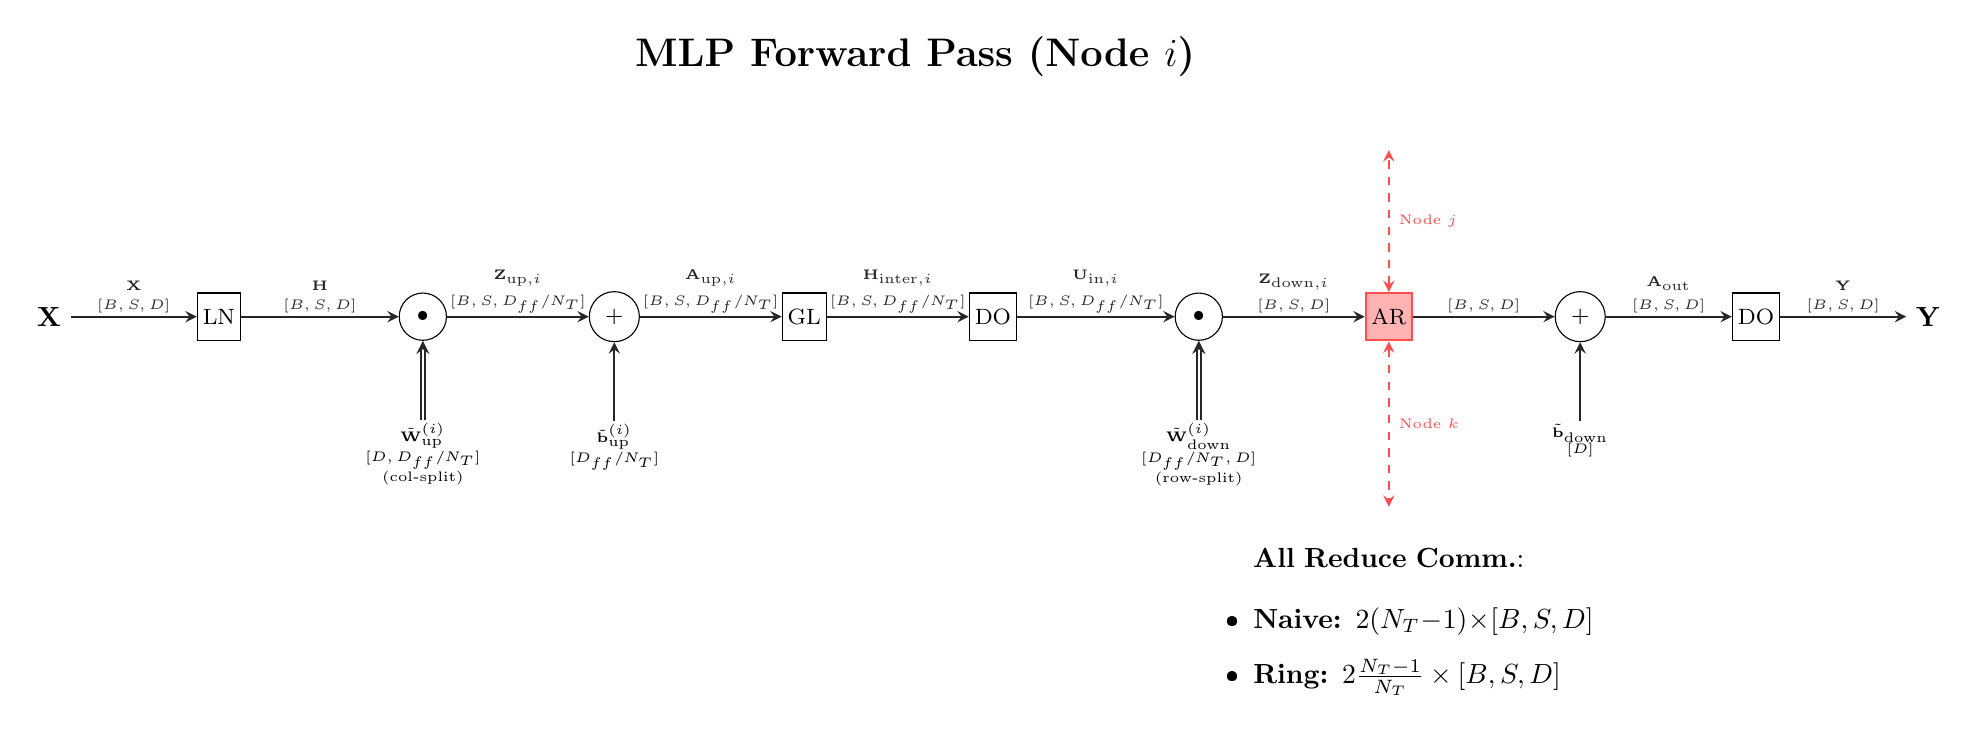
\begin{tikzpicture}[
    >=stealth,
    auxnode/.style={draw, rectangle, fill=white, minimum height=6mm, inner sep=2pt, font=\footnotesize, align=center},
    mulnode/.style={draw, circle, fill=white, minimum size=6mm, font=\footnotesize, align=center},
    addnode/.style={draw, circle, fill=white, minimum size=6mm, font=\footnotesize, align=center},
    allreduce/.style={draw, rectangle, fill=red!30, minimum height=6mm, inner sep=2pt, font=\footnotesize, align=center, thick, draw=red!70},
    sumnode/.style={draw, circle, fill=white, minimum size=6mm, font=\tiny, align=center},
    flow/.style={->, thick, black!85},
    flow2/.style={double, ->, thick, black!85},
    commflow/.style={<->, thick, red!70, dashed},
    dimlabel/.style={font=\tiny, inner sep=1pt, align=center}
]
    \node[font=\Large\bfseries] at (11, 2.8) {MLP Forward Pass (Node $i$)};

    \pgfmathsetmacro{\verticaloffset}{-0.5}

    \node            (MIn)   at (0,\verticaloffset) {$\mathbf{X}$};
    \node[auxnode]   (LN2)   [right=1.6cm of MIn] {LN};
    \node[mulnode]   (L1Mul) [right=2.0cm of LN2] {$\bullet$};
    \node[dimlabel]  (Wup)   [below=1.0cm of L1Mul] {$\tilde{\mathbf{W}}_{\text{up}}^{(i)}$\\$[D, D_{ff}/N_T]$\\(col-split)};
    \node[addnode]   (AddB1) [right=1.8cm of L1Mul] {+};
    \node[dimlabel]  (Bup)   [below=1.0cm of AddB1] {$\tilde{\mathbf{b}}_{\text{up}}^{(i)}$\\$[D_{ff}/N_T]$};
    \node[auxnode]   (Act)   [right=1.8cm of AddB1] {GL};
    \node[auxnode]   (Drop1) [right=1.8cm of Act] {DO};
    \node[mulnode]   (L2Mul) [right=2.0cm of Drop1] {$\bullet$};
    \node[dimlabel]  (Wdown) [below=1.0cm of L2Mul] {$\tilde{\mathbf{W}}_{\text{down}}^{(i)}$\\$[D_{ff}/N_T, D]$\\(row-split)};
    \node[allreduce] (AR)    [right=1.8cm of L2Mul] {AR};
    \node[
      align=center,
      below=2.5cm of AR,
      text width=5.2cm
    ] (AR_info) {%
      \textbf{All Reduce Comm.}:\\[2pt]
      \begin{itemize}
        \item \textbf{Naive:} $2(N_T-1) \times [B,S,D]$
        \item \textbf{Ring:} $2\frac{N_T-1}{N_T} \times [B,S,D]$
      \end{itemize}
    };
    \node[addnode]   (AddB2) [right=1.8cm of AR] {+};
    \node[dimlabel]  (Bdown) [below=1.0cm of AddB2] {$\tilde{\mathbf{b}}_{\text{down}}$\\$[D]$};
    \node[auxnode]   (Drop2) [right=1.6cm of AddB2] {DO};
    \node            (MOut)  [right=1.6cm of Drop2] {$\mathbf{Y}$};

    % All-Reduce communication arrows
    \draw[commflow] (AR.north) -- ++(0, 1.8) node[midway, right, font=\tiny]{Node $j$};
    \draw[commflow] (AR.south) -- ++(0, -2.1) node[midway, right, font=\tiny]{Node $k$};

    \draw[flow] (MIn) -- (LN2) node[dimlabel, midway, above]{\shortstack{$\mathbf{X}$\\$[B,S,D]$}};
    \draw[flow] (LN2) -- (L1Mul) node[dimlabel, midway, above]{\shortstack{$\mathbf{H}$\\$[B,S,D]$}};
    \draw[flow2] (Wup) -- (L1Mul);
    \draw[flow] (L1Mul) -- (AddB1) node[dimlabel, midway, above]{\shortstack{$\mathbf{Z}_{\text{up},i}$\\$[B,S,D_{ff}/N_T]$}};
    \draw[flow] (Bup) -- (AddB1);
    \draw[flow] (AddB1) -- (Act) node[dimlabel, midway, above]{\shortstack{$\mathbf{A}_{\text{up},i}$\\$[B,S,D_{ff}/N_T]$}};
    \draw[flow] (Act) -- (Drop1) node[dimlabel, midway, above]{\shortstack{$\mathbf{H}_{\text{inter},i}$\\$[B,S,D_{ff}/N_T]$}};
    \draw[flow] (Drop1) -- (L2Mul) node[dimlabel, midway, above]{\shortstack{$\mathbf{U}_{\text{in},i}$\\$[B,S,D_{ff}/N_T]$}};
    \draw[flow2] (Wdown) -- (L2Mul);
    \draw[flow] (L2Mul) -- (AR) node[dimlabel, midway, above]{\shortstack{$\mathbf{Z}_{\text{down},i}$\\$[B,S,D]$}};
    \draw[flow] (AR) -- (AddB2) node[dimlabel, midway, above]{\shortstack{$[B,S,D]$}};
    \draw[flow] (Bdown) -- (AddB2);
    \draw[flow] (AddB2) -- (Drop2) node[dimlabel, midway, above]{\shortstack{$\mathbf{A}_{\text{out}}$\\$[B,S,D]$}};
    \draw[flow] (Drop2) -- (MOut) node[dimlabel, midway, above]{\shortstack{$\mathbf{Y}$\\$[B,S,D]$}};

\end{tikzpicture}%
}
  \caption{MLP forward pass with tensor parallelism. The up-projection is
  implemented as a column-parallel linear so that each device holds a
  subset of the intermediate features. The down-projection is
  row-parallel, and an All-Reduce over devices reconstructs the full
  $\mathbf{Z}_{\text{down}}$, after which dropout and the residual
  connection are applied locally.}
  \label{fig:mlp_forward_tp}
\end{figure}

\subsubsection{Backward Pass}

The backward pass for the tensor-parallel MLP reuses the same structure as
the single-node backward graph (Figure~\ref{fig:single_node_mlp_backward}),
but with sharded parameters and explicit All-Reduce operations.

Starting from $\mathrm{d}\mathbf{Y}$ on each device:

\begin{enumerate}
  \item \textbf{Residual and dropout backward}: as before, gradients are
        split between the identity path and the path through the final
        dropout, yielding $\mathrm{d}\mathbf{Z}_{\text{down}}$ on each
        device.
  \item \textbf{Down-projection backward (row-parallel)}: each device
        computes local gradients
        $\mathrm{d}\mathbf{U}^{(t)}$ and parameter gradients
        $\mathrm{d}W_{\text{down}}^{(t)}, \mathrm{d}\mathbf{b}_{\text{down}}^{(t)}$
        using its own shard $W_{\text{down}}^{(t)}$ and local activations
        $\mathbf{U}^{(t)}$. No communication is needed to form
        $\mathrm{d}\mathbf{U}^{(t)}$.
  \item \textbf{Activation backward}: the non-linearity $\phi$ is
        inverted elementwise on each device to obtain
        $\mathrm{d}\mathbf{Z}_{\text{up}}^{(t)}$.
  \item \textbf{Up-projection backward (column-parallel)}:
        for the column-parallel up-projection, each device computes local
        contributions to the gradient with respect to $W_{\text{up}}^{(t)}$
        and a partial gradient w.r.t.\ the input $\mathrm{d}\mathbf{H}^{(t)}$.
        Because $\mathbf{H}$ is shared across devices, we must sum these
        partial gradients:
        \[
          \mathrm{d}\mathbf{H}
            = \sum_{t=0}^{N_T-1} \mathrm{d}\mathbf{H}^{(t)},
        \]
        implemented as an All-Reduce over $t$.
  \item \textbf{Layer normalization backward (if present)}: if the MLP is
        preceded by a layer normalization (as in a pre-LN Transformer),
        its backward pass is applied locally using the aggregated
        $\mathrm{d}\mathbf{H}$.
\end{enumerate}

Figure~\ref{fig:mlp_backward_tp} shows these steps, highlighting the
All-Reduce on $\mathrm{d}\mathbf{H}$ (the only collective required in the
MLP backward pass).

\begin{figure}[htbp]
  % no \centering here to avoid compilation issues
  \resizebox{\linewidth}{!}{%
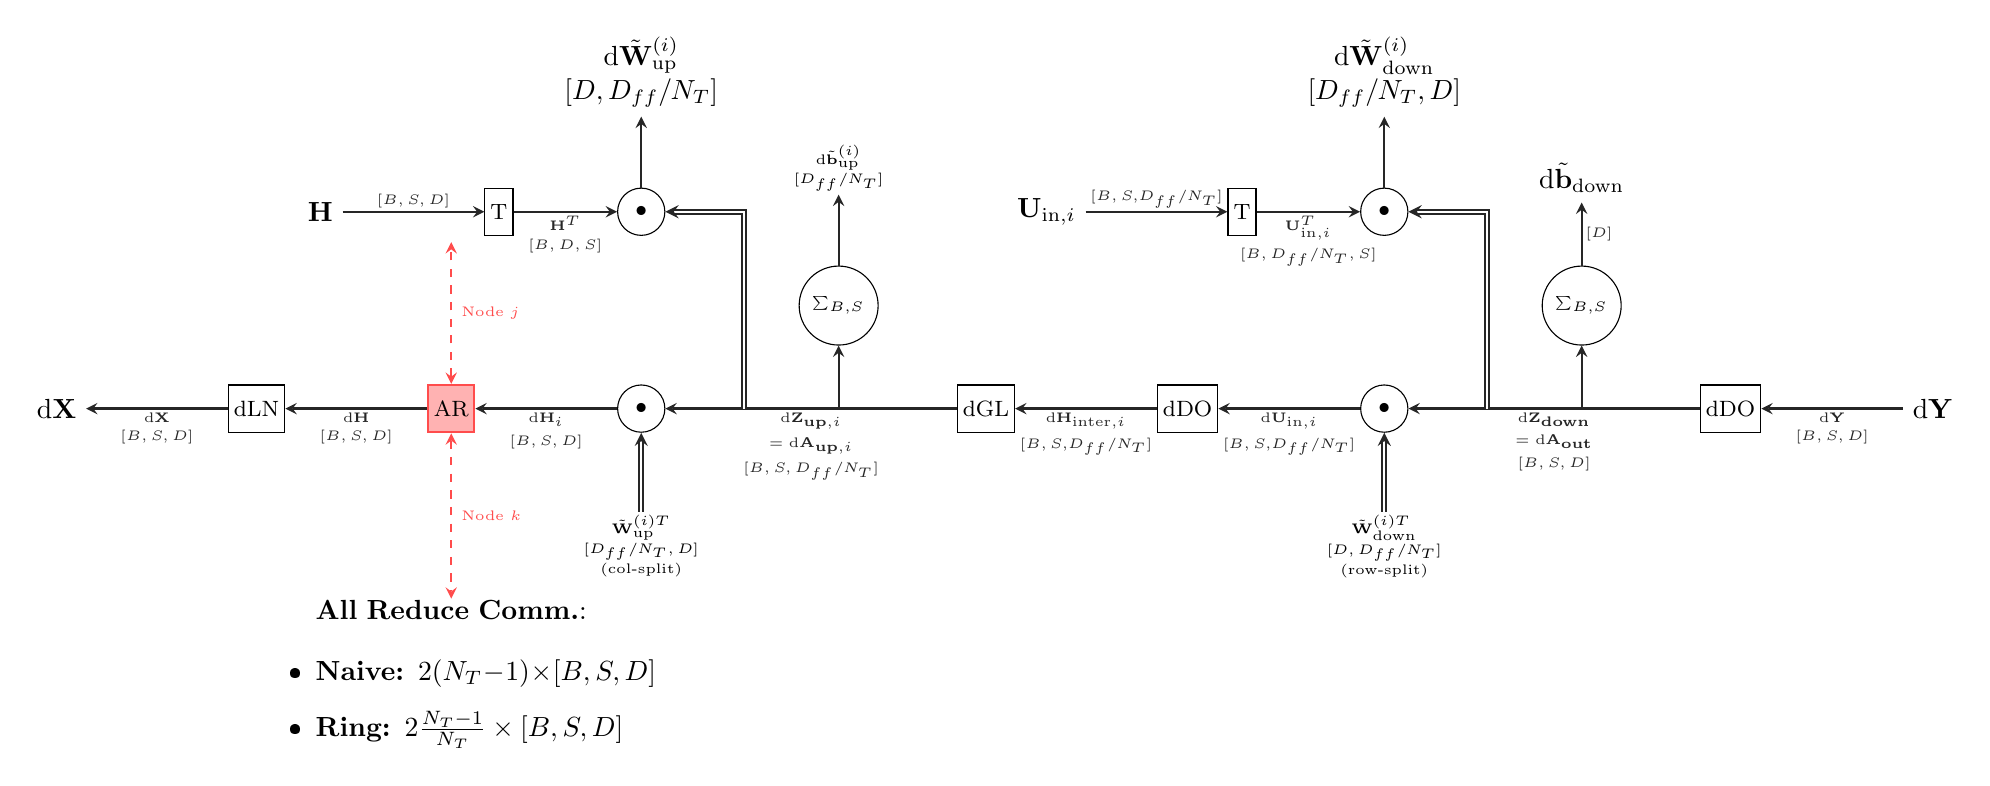
\begin{tikzpicture}[
    >=stealth,
    auxnode/.style={draw, rectangle, fill=white, minimum height=6mm, inner sep=2pt, font=\footnotesize, align=center},
    mulnode/.style={draw, circle, fill=white, minimum size=6mm, font=\footnotesize, align=center},
    addnode/.style={draw, circle, fill=white, minimum size=6mm, font=\footnotesize, align=center},
    sumnode/.style={draw, circle, fill=white, minimum size=6mm, font=\tiny, align=center},
    allreduce/.style={draw, rectangle, fill=red!30, minimum height=6mm, inner sep=2pt, font=\footnotesize, align=center, thick, draw=red!70},
    flow_rev/.style={<-, thick, black!85},
    flow_dw/.style={->, thick, black!85},
    flow_act/.style={double, ->, thick, black!85},
    commflow/.style={<->, thick, red!70, dashed},
    dimlabel/.style={font=\tiny, inner sep=1pt, align=center},
    gradlabel/.style={font=\tiny\bfseries, inner sep=1pt, align=center}
]
    % \node[font=\Large\bfseries] at (5, 10) {MLP Backward Pass (Node $i$)};

    \pgfmathsetmacro{\backwardoffset}{0.0}

    \node (d_MOut) at (12.6, \backwardoffset) {$\mathrm{d}\mathbf{Y}$};
    \node[auxnode] (d_Drop2) [left=1.8cm of d_MOut] {dDO};
    \draw[flow_rev] (d_Drop2) -- (d_MOut)
      node[dimlabel, midway, below]{\shortstack{$\mathrm{d}\mathbf{Y}$\\$[B,S,D]$}};

    \coordinate (split2) at ($(d_Drop2.west) + (-1.5cm, 0)$);
    \coordinate (branch_dUproj) at ($(split2) + (-1.2cm, 0)$);

    \node[sumnode] (d_SumB2) [above=0.8cm of split2] {$\sum_{B, S}$};
    \node (d_Bdown) [above=0.8cm of d_SumB2] {$\mathrm{d}\tilde{\mathbf{b}}_{\text{down}}$};
    \draw[flow_dw] (d_SumB2) -- (d_Bdown) node[dimlabel, midway, right]{$[D]$};

    \draw[flow_rev] (d_SumB2) -- (split2);

    \node[mulnode] (d_L2Mul_in) [left=2.2cm of split2] {$\bullet$};
    \draw[flow_rev] (d_L2Mul_in) -- (d_Drop2)
      node[gradlabel, midway, below]{\shortstack{$\mathrm{d}\mathbf{Z}_{\text{down}}$\\$=\mathrm{d}\mathbf{A}_{\text{out}}$\\$[B,S,D]$}};

    \node[dimlabel] (W_down_T) [align=center, below=1.0cm of d_L2Mul_in] {$\tilde{\mathbf{W}}_{\text{down}}^{(i)T}$\\$[D, D_{ff}/N_T]$\\(row-split)};
    \draw[flow_act] (W_down_T.north) -- (d_L2Mul_in);

    \coordinate (L2Mul_w_y) at ($(d_L2Mul_in) + (0, 2.5cm)$);
    \node[mulnode] (d_L2Mul_w) at (L2Mul_w_y) {$\bullet$};
    \node (d_Wdown) [align=center, above=0.9cm of d_L2Mul_w] {$\mathrm{d}\tilde{\mathbf{W}}_{\text{down}}^{(i)}$\\$[D_{ff}/N_T, D]$};
    \draw[flow_dw] (d_L2Mul_w) -- (d_Wdown);

    \draw[flow_act] (branch_dUproj.north) |- (d_L2Mul_w.east);

    \node[auxnode] (Uin_T) at ($(d_L2Mul_w.west) + (-1.5cm, 0)$) {T};
    \draw[flow_dw] (Uin_T) -- (d_L2Mul_w)
      node[dimlabel, midway, below]{\shortstack{$\mathbf{U}_{\text{in},i}^T$\\$[B, D_{ff}/N_T, S]$}};
    \node (Uin_aux) [left=1.8cm of Uin_T] {$\mathbf{U}_{\text{in},i}$};
    \draw[flow_dw] (Uin_aux) -- (Uin_T) node[dimlabel, midway, above]{\shortstack{$[B,S,$$D_{ff}/N_T]$}};

    \node[auxnode] (d_Drop1) [left=1.8cm of d_L2Mul_in] {dDO};
    \draw[flow_rev] (d_Drop1) -- (d_L2Mul_in)
      node[dimlabel, midway, below]{\shortstack{$\mathrm{d}\mathbf{U}_{\text{in},i}$\\$[B,S,$$D_{ff}/N_T]$}};

    \node[auxnode] (d_Act) [left=1.8cm of d_Drop1] {dGL};
    \draw[flow_rev] (d_Act) -- (d_Drop1)
      node[dimlabel, midway, below]{\shortstack{$\mathrm{d}\mathbf{H}_{\text{inter},i}$\\$[B,S,$$D_{ff}/N_T]$}};

    \coordinate (split1) at ($(d_Act.west) + (-1.5cm, 0)$);
    \coordinate (branch_dHpre) at ($(split1) + (-1.2cm, 0)$);

    \node[sumnode] (d_SumB1) [above=0.8cm of split1] {$\sum_{B, S}$};
    \node[dimlabel] (d_Bup) [above=0.9cm of d_SumB1] {$\mathrm{d}\tilde{\mathbf{b}}_{\text{up}}^{(i)}$\\$[D_{ff}/N_T]$};
    \draw[flow_dw] (d_SumB1) -- (d_Bup);

    \draw[flow_rev] (d_SumB1) -- (split1);

    \node[mulnode] (d_L1Mul_in) [left=2.2cm of split1] {$\bullet$};
    \draw[flow_rev] (d_L1Mul_in) -- (d_Act)
      node[gradlabel, midway, below]{\shortstack{$\mathrm{d}\mathbf{Z}_{\text{up},i}$\\$=\mathrm{d}\mathbf{A}_{\text{up},i}$\\$[B,S,D_{ff}/N_T]$}};

    \node[dimlabel] (W_up_T) [align=center, below=1.0cm of d_L1Mul_in] {$\tilde{\mathbf{W}}_{\text{up}}^{(i)T}$\\$[D_{ff}/N_T, D]$\\(col-split)};
    \draw[flow_act] (W_up_T.north) -- (d_L1Mul_in);

    \coordinate (L1Mul_w_y) at ($(d_L1Mul_in) + (0, 2.5cm)$);
    \node[mulnode] (d_L1Mul_w) at (L1Mul_w_y) {$\bullet$};
    \node (d_Wup) [align=center, above=0.9cm of d_L1Mul_w] {$\mathrm{d}\tilde{\mathbf{W}}_{\text{up}}^{(i)}$\\$[D, D_{ff}/N_T]$};
    \draw[flow_dw] (d_L1Mul_w) -- (d_Wup);

    \draw[flow_act] (branch_dHpre.north) |- (d_L1Mul_w.east);

    \node[auxnode] (Znorm_T) at ($(d_L1Mul_w.west) + (-1.5cm, 0)$) {T};
    \draw[flow_dw] (Znorm_T) -- (d_L1Mul_w)
      node[dimlabel, midway, below]{\shortstack{$\mathbf{H}^T$\\$[B, D, S]$}};
    \node (Znorm_aux) [left=1.8cm of Znorm_T] {$\mathbf{H}$};
    \draw[flow_dw] (Znorm_aux) -- (Znorm_T) node[dimlabel, midway, above]{\shortstack{$[B,S,D]$}};

    \node[allreduce] (AR) [left=1.8cm of d_L1Mul_in] {AR};
    \node[
      align=center,
      below=2.0cm of AR,
      text width=5.2cm
    ] (AR_info) {%
      \textbf{All Reduce Comm.}:\\[2pt]
      \begin{itemize}
        \item \textbf{Naive:} $2(N_T-1) \times [B,S,D]$
        \item \textbf{Ring:} $2\frac{N_T-1}{N_T} \times [B,S,D]$
      \end{itemize}
    };

    % All-Reduce communication arrows
    \draw[commflow] (AR.north) -- ++(0, 1.8) node[midway, right, font=\tiny]{Node $j$};
    \draw[commflow] (AR.south) -- ++(0, -2.1) node[midway, right, font=\tiny]{Node $k$};

    \draw[flow_rev] (AR) -- (d_L1Mul_in)
      node[dimlabel, midway, below]{\shortstack{$\mathrm{d}\mathbf{H}_i$\\$[B,S,D]$}};

    \node[auxnode] (d_LN2) [left=1.8cm of AR] {dLN};
    \draw[flow_rev] (d_LN2) -- (AR)
      node[dimlabel, midway, below]{\shortstack{$\mathrm{d}\mathbf{H}$\\$[B,S,D]$}};

    \node (d_MIn) [left=1.8cm of d_LN2] {$\mathrm{d}\mathbf{X}$};
    \draw[flow_rev] (d_MIn) -- (d_LN2)
      node[dimlabel, midway, below]{\shortstack{$\mathrm{d}\mathbf{X}$\\$[B,S,D]$}};
\end{tikzpicture}%
}
  \caption{MLP backward pass with tensor parallelism. Each device
  backpropagates through its local up- and down-projection shards. The
  only collective in the backward path is an All-Reduce that sums the
  partial input gradients $\mathrm{d}\mathbf{H}^{(t)}$ across devices to
  obtain the full $\mathrm{d}\mathbf{H}$. Parameter gradients remain
  local to each shard.}
  \label{fig:mlp_backward_tp}
\end{figure}


% ------------------------ 6.3 Communication Summary ------------------
\subsection{Communication Patterns and Costs}

Finally, we summarize where collective communication appears in the
tensor-parallel Transformer layer:

\begin{itemize}
  \item \textbf{MHA forward:}
        an All-Reduce after the row-parallel output projection to obtain
        $\mathbf{A}_{\text{lin}}$ on every device
        (Figure~\ref{fig:mha_forward_tp}).
  \item \textbf{MHA backward:}
        an All-Reduce on $\mathrm{d}\mathbf{X}_{\text{norm}}$ to sum
        gradient contributions from all Q/K/V shards
        (Figure~\ref{fig:mha_backward_tp}).
  \item \textbf{MLP forward:}
        an All-Reduce after the row-parallel down-projection to form
        $\mathbf{Z}_{\text{down}}$
        (Figure~\ref{fig:mlp_forward_tp}).
  \item \textbf{MLP backward:}
        an All-Reduce on the input gradient $\mathrm{d}\mathbf{H}$ from
        the column-parallel up-projection
        (Figure~\ref{fig:mlp_backward_tp}).
\end{itemize}

In all cases, the local computation on each device is structurally
identical to the single-node computation described in Section~\ref{sec:sn}; only the
placement of collectives and the sharding of weights and activations
differ. This makes tensor parallelism a natural extension of the
single-node Transformer, well suited for large models that do not fit into
the memory of a single accelerator.

\fi
\clearpage

% ==========================================================
% 7. Data Parallelism (DP)
% ==========================================================
\ifkorean
  % ==========================================================
% 7. 데이터 병렬화
% ==========================================================
\section{데이터 병렬화}
\label{sec:dp}

데이터 병렬화(data parallelism, DP)에서는 각 복제본(replica)이
모델 전체를 그대로 한 벌씩 가지고 있지만, 서로 다른 배치 조각을
처리한다. 개념적으로는 각 디바이스가 단일 노드 설정
(Section~\ref{sec:sn})과 \emph{동일한} 순전파·역전파 계산을 수행하되,
입력 미니배치만 서로 다른 셈이다. 역전파가 끝난 뒤에는
All-Reduce를 통해 기울기를 복제본들 사이에서 동기화하여,
전역 배치를 한 번에 처리하는 단일 노드 학습과
\emph{동일한} 옵티마이저 업데이트가 이루어지도록 한다.

단일 복제본의 관점에서 보면, 각 트랜스포머 블록 안의 순전파 계산 그래프는
단일 노드의 그래프(Section~\ref{sec:sn})와 완전히 같고,
텐서 병렬화(Section~\ref{sec:tp})까지 함께 사용하는 경우에도
각 복제본은 동일한 TP가 적용된 그래프를 자신의 미니배치에 대해 실행한다.
달라지는 것은 입력 배치뿐이다.
글로벌 배치
\[
  \mathbf{X} \in \mathbb{R}^{B \times S \times D}
\]
대신, 복제본 $d$는
\[
  \mathbf{X}_d \in \mathbb{R}^{B_{\text{local}} \times S \times D}
\]
라는 로컬 배치를 보게 되며, $B_{\text{local}} = B / N_D$이다.

데이터 병렬 복제본의 개수를 $N_D$라 두고,
디바이스 인덱스는 $d \in \{0,\dots,N_D-1\}$로 표기한다.

\textbf{핵심 아이디어는 다음과 같다.}
\begin{itemize}
  \item 각 디바이스는 모델 파라미터(가중치와 옵티마이저 상태)를
        \emph{온전히} 한 벌씩 가진다.
  \item 전역 배치 크기 $B$는 $N_D$개의 로컬 배치로 나뉘며,
        각 로컬 배치의 크기는 $B_{\text{local}} = B / N_D$이다.
  \item 각 디바이스의 순전파는 Section~\ref{sec:sn}의 단일 노드 계산과 동일하지만,
        자신의 로컬 배치만 사용한다.
  \item 역전파는 각 디바이스에서 로컬 기울기
        $\nabla W^{(d)}$를 계산한다.
  \item 모든 데이터 병렬 복제본에 걸쳐 All-Reduce를 수행해
        기울기를 평균(또는 합산)함으로써,
        배치 크기 $B$인 단일 노드 실행과 동등한 업데이트를 만든다.
\end{itemize}

텐서 병렬화(Section~\ref{sec:tp})와 달리,
데이터 병렬화는 가중치 행렬이나 활성값을 쪼개지 않는다.
대신 모델 전체는 복제하고, \emph{데이터만} 분할한다.

% ------------------------ 7.1 Overall DP Flow -------------------------
\subsection{데이터 병렬 학습 전체 흐름}

Figure~\ref{fig:dp_overall_flow}는 트랜스포머 레이어에
데이터 병렬화를 적용했을 때의 상위 수준 구조를 보여준다.
단일 노드 개요 그림(Figure~\ref{fig:single_node_overall})과 비교해 보면,
이제 $N_D$개의 서로 동일한 블록 복제본이 있고,
각 복제본이 서로 다른 입력 조각 $\mathbf{X}_d$를 처리하여
로컬 예측과 로컬 손실을 만든다는 점만 다르다.

하나의 학습 스텝에서 수행되는 순서는 다음과 같다.

\begin{enumerate}
  \item \textbf{배치 분할 (batch sharding).}
        전역 배치 크기 $B$를 $N_D$개의 로컬 배치로 나눈다.
        각 로컬 배치의 크기는 $B_{\text{local}}$이다:
        \[
          \{\mathbf{X}_0,\dots,\mathbf{X}_{N_D-1}\},
          \qquad
          \mathbf{X}_d \in \mathbb{R}^{B_{\text{local}} \times S \times D_{\text{in}}}.
        \]
        각 디바이스 $d$는 이에 대응하는 타깃 토큰
        $\mathbf{Y}_d$도 함께 받는다.
  \item \textbf{로컬 순전파.}
        각 디바이스는 자신의 로컬 입력 $\mathbf{X}_d$에 대해
        전체 트랜스포머 스택(입력 임베딩, MHA, MLP, 출력 프로젝션)을
        Section~\ref{sec:sn}에서와 동일하게 적용한다.
        텐서 병렬화(Section~\ref{sec:tp})도 함께 사용하는 경우,
        각 복제본은 $\mathbf{X}_d$에 대해 동일한 TP-적용 그래프를 실행한다.
        어떤 경우든 순전파 구조 자체는 변하지 않고,
        달라지는 것은 배치 차원과 기울기 동기화의 존재 여부뿐이다.
        각 디바이스는 로컬 로그릿, 확률, 손실 $\mathcal{L}_d$를 만든다.
  \item \textbf{로컬 역전파.}
        각 디바이스에서 손실 $\mathcal{L}_d$에 대한 역전파를 수행하여,
        디바이스 $d$에 있는 모든 파라미터에 대한 로컬 기울기
        $\nabla W^{(d)}$를 얻는다.
  \item \textbf{기울기 동기화 (All-Reduce).}
        각 파라미터 텐서 $W$에 대해 데이터 병렬 그룹 전체에 대해
        All-Reduce를 수행한다:
        \[
          \nabla W
            = \frac{1}{N_D}
              \sum_{d=0}^{N_D-1} \nabla W^{(d)}.
        \]
        이 단계 이후에는 모든 복제본이 동일한 평균 기울기
        $\nabla W$를 갖게 된다.
  \item \textbf{옵티마이저 업데이트.}
        각 디바이스는 자신의 로컬 파라미터 복사본에
        동일한 옵티마이저(SGD, Adam 등)를 적용하여 업데이트한다.
        기울기가 동기화되어 있기 때문에,
        모든 복제본의 파라미터는 다시 일치하게 된다.
\end{enumerate}

Figure~\ref{fig:dp_overall_flow}에서는 이러한 과정을
단일 트랜스포머 레이어 관점에서 요약한다.
각 디바이스는 단일 노드 그래프의 \emph{완전한} 복사본을 가지고 있으며,
기울기 All-Reduce 단계만 추가된다.

\begin{figure}[htbp]
  \centering
  \resizebox{\linewidth}{!}{%
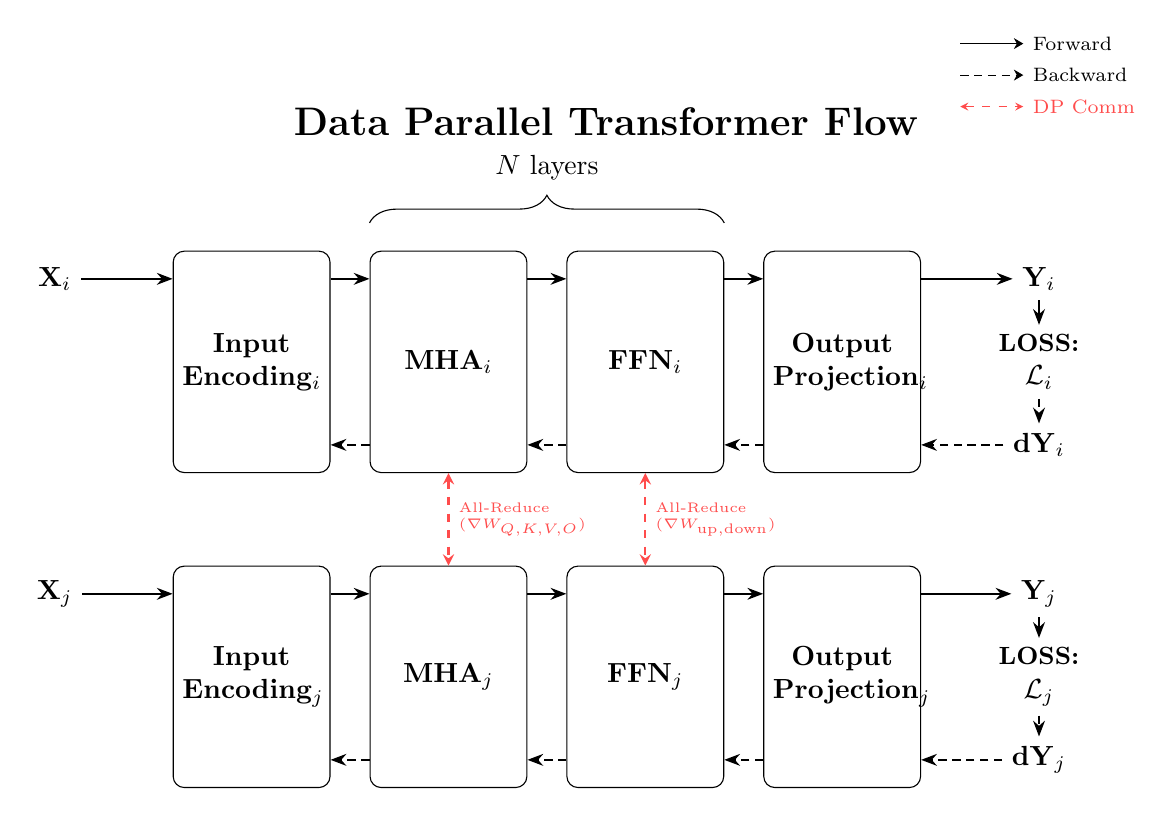
\begin{tikzpicture}[
    node distance=2.5cm,
    >=stealth,
    block/.style={rectangle, draw=black, fill=white, text width=5em, text centered, rounded corners, minimum height=8em, font=\bfseries},
    forward/.style={-{Stealth[length=2mm]}, thick, black},
    backward/.style={-{Stealth[length=2mm]}, thick, black, densely dashed},
    dpcomm/.style={<->, thick, red!70, dashed},
    io/.style={text centered, font=\bfseries}
]
    % Title
    \node[font=\Large\bfseries] at (7, 12) {Data Parallel Transformer Flow};

    % ========== Node i (Upper) ==========
    \node (input_i) [io] at (0, 10) {$\mathbf{X}_i$};
    \node (encoding_i) [block, right of=input_i, yshift=-3em] {Input\\Encoding$_i$};
    \node (mha_i) [block, right of=encoding_i] {MHA$_i$};
    \node (mlp_i) [block, right of=mha_i] {FFN$_i$};
    \node (output_i) [block, right of=mlp_i] {Output\\Projection$_i$};
    \node (pred_i) [io, right of=output_i, yshift=3em] {$\mathbf{Y}_i$};
    \node (loss_i) [align=center, io, right of=output_i] {\small LOSS:\\$\mathcal{L}_i$};
    \node (gradient_i) [io, right of=output_i, yshift=-3em] {$\mathbf{dY}_i$};

    % Forward arrows - Node i
    \draw [forward] (input_i) -- ([yshift=3em]encoding_i.west);
    \draw [forward] ([yshift=3em]encoding_i.east) -- ([yshift=3em]mha_i.west);
    \draw [forward] ([yshift=3em]mha_i.east) -- ([yshift=3em]mlp_i.west);
    \draw [forward] ([yshift=3em]mlp_i.east) -- ([yshift=3em]output_i.west);
    \draw [forward] ([yshift=3em]output_i.east) -- (pred_i);
    \draw [forward] (pred_i) -- (loss_i);
    \draw [backward] (loss_i) -- (gradient_i);

    % Backward arrows - Node i
    \draw [backward] (gradient_i) -- ([yshift=-3em]output_i.east);
    \draw [backward] ([yshift=-3em]output_i.west) -- ([yshift=-3em]mlp_i.east);
    \draw [backward] ([yshift=-3em]mlp_i.west) -- ([yshift=-3em]mha_i.east);
    \draw [backward] ([yshift=-3em]mha_i.west) -- ([yshift=-3em]encoding_i.east);

    % Brace for layer repetition - Node i
    \draw[decorate, decoration={brace, amplitude=10pt}]
        ([yshift=1.0em]mha_i.north west) -- ([yshift=1.0em]mlp_i.north east)
        node[midway, above=12pt, font=\normalsize] {$N$ layers};

    % ========== Node j (Lower) ==========
    \node (input_j) [io] at (0, 6) {$\mathbf{X}_j$};
    \node (encoding_j) [block, right of=input_j, yshift=-3em] {Input\\Encoding$_j$};
    \node (mha_j) [block, right of=encoding_j] {MHA$_j$};
    \node (mlp_j) [block, right of=mha_j] {FFN$_j$};
    \node (output_j) [block, right of=mlp_j] {Output\\Projection$_j$};
    \node (pred_j) [io, right of=output_j, yshift=3em] {$\mathbf{Y}_j$};
    \node (loss_j) [align=center, io, right of=output_j] {\small LOSS:\\$\mathcal{L}_j$};
    \node (gradient_j) [io, right of=output_j, yshift=-3em] {$\mathbf{dY}_j$};

    % Forward arrows - Node j
    \draw [forward] (input_j) -- ([yshift=3em]encoding_j.west);
    \draw [forward] ([yshift=3em]encoding_j.east) -- ([yshift=3em]mha_j.west);
    \draw [forward] ([yshift=3em]mha_j.east) -- ([yshift=3em]mlp_j.west);
    \draw [forward] ([yshift=3em]mlp_j.east) -- ([yshift=3em]output_j.west);
    \draw [forward] ([yshift=3em]output_j.east) -- (pred_j);
    \draw [forward] (pred_j) -- (loss_j);
    \draw [backward] (loss_j) -- (gradient_j);

    % Backward arrows - Node j
    \draw [backward] (gradient_j) -- ([yshift=-3em]output_j.east);
    \draw [backward] ([yshift=-3em]output_j.west) -- ([yshift=-3em]mlp_j.east);
    \draw [backward] ([yshift=-3em]mlp_j.west) -- ([yshift=-3em]mha_j.east);
    \draw [backward] ([yshift=-3em]mha_j.west) -- ([yshift=-3em]encoding_j.east);

    % ========== DP Communications ==========
    \draw [dpcomm] (mha_i.south) -- (mha_j.north) node[midway, right, font=\tiny, align=left] {All-Reduce\\$(\nabla W_{Q,K,V,O})$};
    \draw [dpcomm] (mlp_i.south) -- (mlp_j.north) node[midway, right, font=\tiny, align=left] {All-Reduce\\$(\nabla W_{\text{up},\text{down}})$};

    % Labels (Legend)
    \coordinate (legend) at ([xshift=11.5cm, yshift=8.5em]input_i);

    % Forward (작은 화살표 + 작은 글자)
    \draw[
        forward,
        -{Stealth[length=1.2mm,width=1.4mm]}, % 화살표 더 작게
        line width=0.3pt                       % 선 더 얇게
    ] (legend) -- ++(0.8,0)
      node[right, font=\scriptsize] {Forward};

    % Backward
    \draw[
        backward,
        -{Stealth[length=1.2mm,width=1.4mm]},
        line width=0.3pt
    ] ([yshift=-0.4cm]legend) -- ++(0.8,0)
      node[right, font=\scriptsize] {Backward};

    % DP Comm
    \draw[
        dpcomm,
        line width=0.3pt
    ] ([yshift=-0.8cm]legend) -- ++(0.8,0)
      node[right, font=\scriptsize] {DP Comm};
\end{tikzpicture}%
}
  \caption{데이터 병렬화가 적용된 트랜스포머 레이어 전체 구조.
  각 디바이스는 모델 전체를 한 벌씩 가지고 있고,
  서로 다른 입력 배치 조각($\mathbf{X}_i$, $\mathbf{X}_j$, \dots)을 처리한다.
  순전파와 역전파는 단일 노드와 동일하게 로컬에서 수행되며,
  각 블록(MHA, MLP, 출력 프로젝션)의 기울기는 All-Reduce를 통해
  복제본 간에 동기화된다.}
  \label{fig:dp_overall_flow}
\end{figure}

% ------------------------ 7.2 Relation to Single-Node -----------------
\subsection{단일 노드 계산과의 관계}

데이터 병렬화는 Section~\ref{sec:sn}의 단일 노드 계산 위에
\emph{래퍼(wrapper)}를 씌운 것으로 보는 것이 이해에 도움이 된다.

\begin{itemize}
  \item \textbf{복제본별 동일한 계산 그래프.}
        어떤 레이어(MHA, MLP, 출력 프로젝션)를 보더라도,
        한 디바이스에서의 순전파·역전파 그래프는
        단일 노드 그림들
        (Figures~\ref{fig:single_node_mha_forward},
         \ref{fig:single_node_mha_backward},
         \ref{fig:single_node_mlp_forward},
         \ref{fig:single_node_mlp_backward} 등)과 동일하다.
        텐서 병렬화가 활성화된 경우에도,
        Section~\ref{sec:tp}에서 설명한 TP 버전 그래프를 그대로 사용하되,
        입력 배치만 $\mathbf{X}_d$로 바뀐다.
  \item \textbf{다른 미니배치.}
        순전파 관점에서의 유일한 차이는 각 복제본이
        전역 배치의 서로 다른 조각을 본다는 점이다.
        데이터 병렬화에서는 순전파 활성값에 대해
        디바이스 간 통신이 필요 없다.
  \item \textbf{기울기 집계만 추가.}
        역전파가 끝난 뒤에만,
        파라미터 기울기를 All-Reduce를 통해 합산/평균한다.
        그 외의 계산 그래프 구조는 단일 노드와 동일하다.
  \item \textbf{큰 배치와의 동등성.}
        기울기를 복제본들 사이에서 평균하면,
        결과 업데이트는 배치 크기
        $B = N_D \cdot B_{\text{local}}$인 단일 노드 실행과
        수학적으로 동등해진다
        (드롭아웃 노이즈 등 미세한 차이는 무시).
\end{itemize}

반대로, 텐서 병렬화(Section~\ref{sec:tp})는
각 레이어 내부의 그래프 자체를 수정한다.
가중치 행렬을 샤딩하고, 순전파·역전파 중간에 집합 통신을 삽입한다.
데이터 병렬화는 레이어 내부의 그래프를 그대로 두고,
\emph{기울기 수준에서만} 통신을 추가하는 방식이라고 볼 수 있다.

% ------------------------ 7.3 MHA Backward under DP -------------------
\subsection{데이터 병렬 환경에서의 MHA 역전파}

MHA 블록에 대한 데이터 병렬 역전파를 보다 구체적으로 살펴보자.
Section~\ref{sec:sn}의 단일 노드 MHA 역전파에서는,
기울기가 출력 프로젝션, 어텐션 연산, Q/K/V 프로젝션,
레이어 정규화를 거꾸로 따라가며
$\nabla W_Q, \nabla W_K, \nabla W_V, \nabla W_O$ 등을 계산한다.

데이터 병렬 환경에서도 \emph{각 복제본 내부}의 계산 그래프는
그림 구조와 텐서 모양까지 단일 노드 MHA 역전파
(Figure~\ref{fig:single_node_mha_backward})와 동일하다.
차이는 다음과 같다.

\begin{itemize}
  \item 각 디바이스 $d$는 자신의 미니배치 $\mathbf{X}_d$에 대해
        로컬 기울기
        $\nabla W_Q^{(d)}, \nabla W_K^{(d)}, \nabla W_V^{(d)}, \nabla W_O^{(d)}$
        를 계산한다.
  \item 그런 다음, 모든 데이터 병렬 복제본에 대해
        All-Reduce를 수행하여 전역 기울기를 얻는다:
        \[
          \nabla W_Q
            = \frac{1}{N_D}
              \sum_{d=0}^{N_D-1} \nabla W_Q^{(d)}, \quad
          \nabla W_K
            = \frac{1}{N_D}
              \sum_{d=0}^{N_D-1} \nabla W_K^{(d)},
        \]
        \[
          \nabla W_V
            = \frac{1}{N_D}
              \sum_{d=0}^{N_D-1} \nabla W_V^{(d)}, \quad
          \nabla W_O
            = \frac{1}{N_D}
              \sum_{d=0}^{N_D-1} \nabla W_O^{(d)}.
        \]
\end{itemize}

이 동기화 이후에는 각 디바이스가
동일한 평균 기울기
$\nabla W_Q, \nabla W_K, \nabla W_V, \nabla W_O$를 가지게 된다.

Figure~\ref{fig:mha_backward_dp}는 이 과정을 그림으로 나타낸다.
MHA 블록 내부의 노드와 텐서 모양은
Figure~\ref{fig:single_node_mha_backward}과 동일하지만,
추가된 박스와 붉은 점선 화살표가
데이터 병렬 복제본 사이에서 기울기를 All-Reduce하는 위치를 표시한다.

\begin{landscape}
\begin{figure}[p]
  % no \centering here to avoid compilation issues
  \resizebox{\linewidth}{!}{%
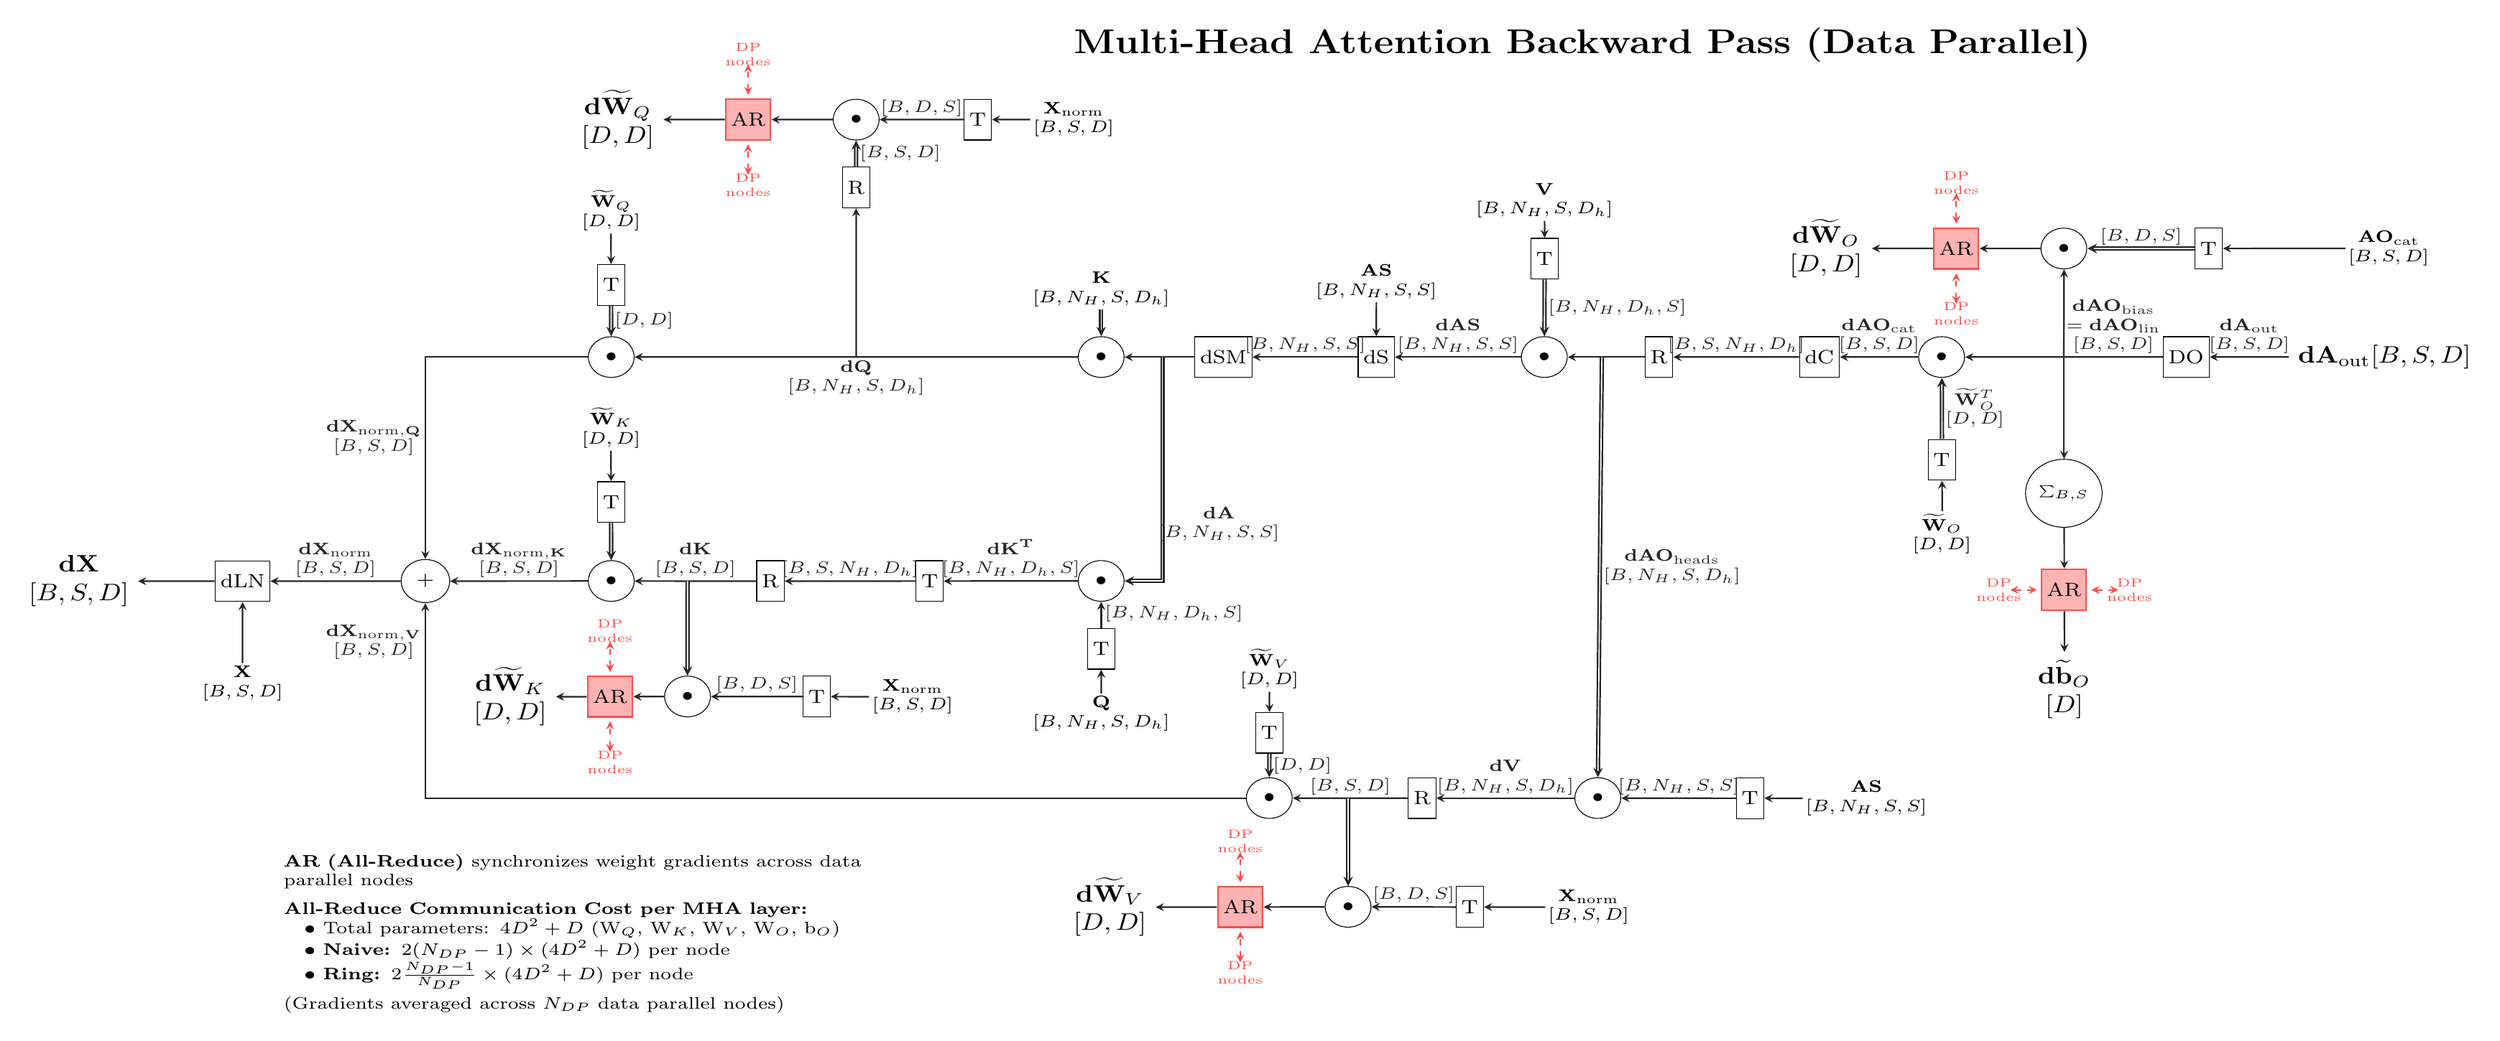
\begin{tikzpicture}[
  every node/.style={transform shape},
  >=stealth,
  auxnode/.style={draw, rectangle, fill=white, minimum height=6mm, inner sep=2pt, font=\footnotesize, align=center},
  mulnode/.style={draw, circle, fill=white, minimum size=6mm, font=\footnotesize, align=center},
  addnode/.style={draw, circle, fill=white, minimum size=6mm, font=\footnotesize, align=center},
  sumnode/.style={draw, circle, fill=white, minimum size=6mm, font=\tiny, align=center},
  arnode/.style={draw, rectangle, fill=red!30, minimum height=6mm, inner sep=2pt, font=\footnotesize, align=center, thick, draw=red!70},
  flow/.style={->, thick, black!85},
  flow2/.style={->, double, thick, black!85},
  dimlabel/.style={font=\scriptsize, inner sep=1pt, align=center},
  gradflow/.style={->, thick, black!85},
  gradweight/.style={->, thick, black!85},
  dpgradweight/.style={->, thick, black!85},
  dpcomm/.style={<->, thick, red!70, dashed}
]

\begin{scope}[xscale=1.35, yscale=1.2]

\def\yoffset{-1.0}
\def\dVXyoffset{-6.5}

\coordinate (Grad_Aout_B) at (17.5, \yoffset);
\coordinate (dDrop_center) at (15.9, \yoffset);
\coordinate (ProjGradSplit) at (14.3, \yoffset);
\coordinate (dOProj_center) at (12.7, \yoffset);
\coordinate (C_center) at (11.1, \yoffset);
\coordinate (R_center) at (9.0, \yoffset);
\coordinate (dPV_AS_calc_center) at (7.5, \yoffset);
\coordinate (dSoft_center) at (5.3, \yoffset);
\coordinate (dSM_calc_center) at (3.3, \yoffset);
\coordinate (dV_calc_center) at (8.2, \dVXyoffset+\yoffset);
\coordinate (R_V_bwd_center) at (5.9, \dVXyoffset+\yoffset);
\coordinate (dVX_calc_center) at (3.9, \dVXyoffset+\yoffset);
\coordinate (dQK_calc_Q_center) at (1.7, \yoffset);
\coordinate (dQK_calc_K_center) at (1.7, -3.3+\yoffset);
\coordinate (K_BWD_input_center) at (1.7, 1.0+\yoffset);
\coordinate (T_Q_bwd_center) at (1.7, -4.3+\yoffset);

\node[font=\Large\bfseries] at (8, 4.6+\yoffset) {Multi-Head Attention Backward Pass (Data Parallel)};

\node (Grad_Aout_B) at (18.5, \yoffset) {$\mathbf{dA}_{\text{out}}$\\$[B,S,D]$};
\node[auxnode] (DO) at (dDrop_center) {DO};
\node[mulnode] (dOProj) at (dOProj_center) {$\bullet$};

\node[auxnode] (T_WO) [below=0.9cm of dOProj] {T};
\node[dimlabel] (WO_BWD) [below=0.45cm of T_WO] {$\widetilde{\mathbf{W}}_{O}$\\$[D,D]$};

\node[mulnode] (dWO_calc) at ($(ProjGradSplit)+(0, 1.6)$) {$\bullet$};

% Add AR node before dWO
\node[arnode] (AR_WO) [left=0.8cm of dWO_calc] {AR};
\draw[dpcomm] ([yshift=-0.5cm]AR_WO.south) -- ([yshift=-0.05cm]AR_WO.south);
\draw[dpcomm] ([yshift=0.05cm]AR_WO.north) -- ([yshift=0.5cm]AR_WO.north);
\node[font=\tiny, red!70, align=center] at ([yshift=-0.65cm]AR_WO.south) {DP\\nodes};
\node[font=\tiny, red!70, align=center] at ([yshift=0.65cm]AR_WO.north) {DP\\nodes};

\node[align=center, left=0.8cm of AR_WO]
  (dWO_GRAD) {$\mathbf{d}\widetilde{\mathbf{W}}_{O}$\\$[D,D]$};
\draw[dpgradweight] (dWO_calc) -- (AR_WO);
\draw[gradflow] (AR_WO) -- (dWO_GRAD);

\node[auxnode] (T_AO_in) [right=1.4cm of dWO_calc] {T};
\node[dimlabel] (AO_in_local_label) [right=1.6cm of T_AO_in] {$\mathbf{AO}_{\text{cat}}$\\$[B,S,D]$};

\node[auxnode] (C) at (C_center) {dC};
\node[auxnode] (R) at (R_center) {R};

\node[mulnode] (dPV_AS_calc) at (dPV_AS_calc_center) {$\bullet$};
\node[auxnode] (dSoft) at (dSoft_center) {dS};
\node[auxnode] (dSM_calc) at (dSM_calc_center) {dSM};

\node[mulnode] (dQK_calc_Q) at (dQK_calc_Q_center) {$\bullet$};
\node[mulnode] (dQX_proj_calc) [left=5.8cm of dQK_calc_Q] {$\bullet$};

\node[mulnode] (dQK_calc_K) at (dQK_calc_K_center) {$\bullet$};
\node[mulnode] (dKX_proj_calc) [left=5.8cm of dQK_calc_K] {$\bullet$};

\node[dimlabel] (K_BWD_input) at (K_BWD_input_center) {$\mathbf{K}$\\$[B,N_H,S,D_h]$};
\node[auxnode] (T_Q_bwd) at (T_Q_bwd_center) {T};
\node[dimlabel] (Q_BWD_input) [below=0.35cm of T_Q_bwd] {$\mathbf{Q}$\\$[B,N_H,S,D_h]$};

\node[dimlabel] (V_FWD) [above=1.7cm of dPV_AS_calc] {$\mathbf{V}$\\$[B,N_H,S,D_h]$};
\node[auxnode] (T_V_bwd) [below=0.25cm of V_FWD] {T};

\node[mulnode] (dV_calc) at (dV_calc_center) {$\bullet$};
\node[auxnode] (T_AS_bwd) [right=1.5cm of dV_calc] {T};
\node[dimlabel] (AS_BWD_for_V) [right=0.5cm of T_AS_bwd] {$\mathbf{AS}$\\$[B,N_H,S,S]$};

\node[auxnode] (R_V_bwd) at (R_V_bwd_center) {R};
\node[mulnode] (dVX_calc) at (dVX_calc_center) {$\bullet$};

\node[auxnode] (T_WV) [above=0.35cm of dVX_calc] {T};
\node[dimlabel] (WV_BWD) [above=0.3cm of T_WV] {$\widetilde{\mathbf{W}}_{V}$\\$[D,D]$};

\node[sumnode] (Sum_dBO) [below=1.5cm of ProjGradSplit] {$\sum_{B, S}$};

% Add AR node before dBO
\node[arnode] (AR_BO) [below=0.6cm of Sum_dBO] {AR};
\draw[dpcomm] ([xshift=-0.4cm]AR_BO.west) -- ([xshift=-0.05cm]AR_BO.west);
\draw[dpcomm] ([xshift=0.05cm]AR_BO.east) -- ([xshift=0.4cm]AR_BO.east);
\node[font=\tiny, red!70, align=center] at ([xshift=-0.55cm]AR_BO.west) {DP\\nodes};
\node[font=\tiny, red!70, align=center] at ([xshift=0.55cm]AR_BO.east) {DP\\nodes};

\node[align=center] (dBO) [below=0.6cm of AR_BO] {$\mathbf{d}\widetilde{\mathbf{b}}_{O}$\\$[D]$};
\draw[dpgradweight] (Sum_dBO) -- (AR_BO);
\draw[gradflow] (AR_BO) -- (dBO);

\draw[gradflow] (Grad_Aout_B) -- (DO)
  node[dimlabel, midway, above]{$\mathbf{dA}_{\text{out}}$\\$[B,S,D]$};

\draw[gradflow] (DO) -- (dOProj)
  node[dimlabel, pos=0.25, above]{$\mathbf{dAO}_{\text{bias}}$\\$=\mathbf{dAO}_{\text{lin}}$\\$[B,S,D]$};

\draw[gradflow] (ProjGradSplit) -- (dWO_calc.south);
\draw[gradflow] (ProjGradSplit) -- ([yshift=-0.75cm]ProjGradSplit) -| (Sum_dBO.north);

\draw[gradflow] (dOProj) -- (C)
  node[dimlabel, midway, above]{$\mathbf{dAO}_{\text{cat}}$\\$[B,S,D]$};
\draw[gradflow] (C) -- (R)
  node[dimlabel, midway, above]{$[B,S,N_H,D_h]$};

\coordinate (R_split_point) at ($(dPV_AS_calc)!0.5!(R)$);
\draw[gradflow] (R.west) -- (dPV_AS_calc.east);
\draw[flow2] (R_split_point) -- (dV_calc.north)
  node[dimlabel, midway, right]{$\mathbf{dAO}_{\text{heads}}$\\$[B,N_H,S,D_h]$};

\draw[gradflow] (V_FWD.south) -- (T_V_bwd.north);
\draw[flow2] (T_V_bwd.south) -- (dPV_AS_calc.north)
  node[dimlabel, midway, right]{$[B,N_H,D_h,S]$};
\draw[gradflow] (dPV_AS_calc.west) -- (dSoft.east)
  node[dimlabel, midway, above]{$\mathbf{dAS}$\\$[B,N_H,S,S]$};

\node (AS_BWD_dS) [dimlabel, above=0.5cm of dSoft] {$\mathbf{AS}$\\$[B,N_H,S,S]$};
\draw[gradflow] (AS_BWD_dS.south) -- (dSoft.north);
\draw[gradflow] (dSoft.west) -- (dSM_calc.east)
  node[dimlabel, midway, above]{$[B,N_H,S,S]$};

\coordinate (dA_Split_X) at ($(dSM_calc_center)!0.5!(dQK_calc_Q_center)$);
\coordinate (dA_Split) at (dA_Split_X |- dQK_calc_Q.east);
\draw[gradflow] (dSM_calc.west) -- (dQK_calc_Q.east);
\draw[flow2] (dA_Split) -- (dA_Split |- dQK_calc_K.east) -- (dQK_calc_K.east)
  node[dimlabel, pos=-1.5, above, yshift=15]{$\mathbf{dA}$\\$[B,N_H,S,S]$};

\draw[flow2] (K_BWD_input.south) -- (dQK_calc_Q.north);
\draw[gradweight] (dQK_calc_Q) -- (dQX_proj_calc)
  node[dimlabel, midway, below]{$\mathbf{dQ}$\\$[B,N_H,S,D_h]$};

\node[auxnode] (T_WQ_bwd) [above=0.45cm of dQX_proj_calc] {T};
\node[dimlabel] (WQ_bwd) [above=0.45cm of T_WQ_bwd] {$\widetilde{\mathbf{W}}_{Q}$\\$[D,D]$};
\draw[flow] (WQ_bwd) -- (T_WQ_bwd);
\draw[flow2] (T_WQ_bwd.south) -- (dQX_proj_calc.north)
  node[dimlabel, midway, right]{$[D,D]$};

\draw[flow] (Q_BWD_input.north) -- (T_Q_bwd.south);
\draw[flow] (T_Q_bwd.north) -- (dQK_calc_K.south)
  node[dimlabel, pos=0.55, right]{$[B,N_H,D_h,S]$};

\node[auxnode] (T_dK) at ($(dQK_calc_K)!0.35!(dKX_proj_calc)$) {T};
\node[auxnode] (R_dK_mid) at ($(T_dK)!0.5!(dKX_proj_calc)$) {R};

\draw[gradweight] (dQK_calc_K) -- (T_dK)
  node[dimlabel, midway, above]{$\mathbf{dK^T}$\\$[B,N_H,D_h,S]$};
\draw[gradweight] (T_dK) -- (R_dK_mid)
  node[dimlabel, midway, above]{$[B,S,N_H,D_h]$};
\draw[gradweight] (R_dK_mid) -- (dKX_proj_calc)
  node[dimlabel, midway, above]{$\mathbf{dK}$\\$[B,S,D]$};

\node[auxnode] (T_WK_bwd) [above=0.55cm of dKX_proj_calc] {T};
\node[dimlabel] (WK_bwd) [above=0.45cm of T_WK_bwd] {$\widetilde{\mathbf{W}}_{K}$\\$[D,D]$};
\draw[gradflow] (WK_bwd) -- (T_WK_bwd);
\draw[flow2] (T_WK_bwd.south) -- (dKX_proj_calc.north);
\draw[gradflow] (AS_BWD_for_V.west) -- (T_AS_bwd.east);
\draw[gradflow] (T_AS_bwd.west) -- (dV_calc.east)
  node[dimlabel, midway, above]{$[B,N_H,S,S]$};
\draw[gradflow] (dV_calc.west) -- (R_V_bwd.east)
  node[dimlabel, midway, above]{$\mathbf{dV}$\\$[B,N_H,S,D_h]$};
\draw[gradflow] (R_V_bwd) -- (dVX_calc.east)
  node[dimlabel, midway, above]{$[B,S,D]$};

\draw[gradflow] (WV_BWD) -- (T_WV);
\draw[flow2] (T_WV) -- (dVX_calc.north)
  node[dimlabel, midway, right]{$[D,D]$};

\node[addnode] (Sum_dXnorm) [left=1.8cm of dKX_proj_calc] {$+$};

\draw[gradweight] (dQX_proj_calc.west) -| node[dimlabel, pos=0.7, left]{$\mathbf{dX}_{\text{norm},\mathbf{Q}}$\\$[B,S,D]$} (Sum_dXnorm.north);
\draw[gradweight] (dKX_proj_calc.west) -- node[dimlabel, midway, above]{$\mathbf{dX}_{\text{norm},\mathbf{K}}$\\$[B,S,D]$} (Sum_dXnorm.east);
\draw[gradweight] (dVX_calc.west) -| node[dimlabel, pos=0.9, left]{$\mathbf{dX}_{\text{norm},\mathbf{V}}$\\$[B,S,D]$} (Sum_dXnorm.south);

\coordinate (dV_branch) at ($(R_V_bwd.west)!0.52!(dVX_calc.east)$);
\node[mulnode] (dWV_mul) at ($(dV_branch)+(0,-1.6cm)$) {$\bullet$};
\draw[flow2] (dV_branch) -- (dWV_mul.north);

\node[auxnode] (T_Xnorm) [right=1.1cm of dWV_mul] {T};
\node[dimlabel] (Xnorm_local) [right=0.8cm of T_Xnorm] {$\mathbf{X}_{\text{norm}}$\\$[B,S,D]$};
\draw[gradflow] (Xnorm_local) -- (T_Xnorm);
\draw[gradflow] (T_Xnorm.west) -- (dWV_mul.east)
  node[dimlabel, midway, above]{$[B,D,S]$};

% Add AR node before dWV
\node[arnode] (AR_WV) [left=0.8cm of dWV_mul] {AR};
\draw[dpcomm] ([yshift=-0.5cm]AR_WV.south) -- ([yshift=-0.05cm]AR_WV.south);
\draw[dpcomm] ([yshift=0.05cm]AR_WV.north) -- ([yshift=0.5cm]AR_WV.north);
\node[font=\tiny, red!70, align=center] at ([yshift=-0.65cm]AR_WV.south) {DP\\nodes};
\node[font=\tiny, red!70, align=center] at ([yshift=0.65cm]AR_WV.north) {DP\\nodes};

\node[align=center] (dWV_out) [left=0.8cm of AR_WV] {$\mathbf{d}\widetilde{\mathbf{W}}_{V}$\\$[D,D]$};
\draw[dpgradweight] (dWV_mul.west) -- (AR_WV);
\draw[gradflow] (AR_WV) -- (dWV_out);

\coordinate (dQ_branch) at ($(dQK_calc_Q.east)!0.50!(dQX_proj_calc.west)$);
\node[mulnode] (dWQ_mul) at ($(dQ_branch)+(0,3.5cm)$) {$\bullet$};
\node[auxnode] (R_dQ_for_WQ) at ($(dWQ_mul)+(0,-1.0cm)$) {R};
\draw[gradflow]  (dQ_branch) -- (R_dQ_for_WQ.south);
\draw[flow2] (R_dQ_for_WQ.north) -- (dWQ_mul.south)
  node[dimlabel, midway, right]{$[B,S,D]$};

\node[auxnode] (T_XnormQ) [right=1.1cm of dWQ_mul] {T};
\node[dimlabel] (Xnorm_localQ) [right=0.5cm of T_XnormQ] {$\mathbf{X}_{\text{norm}}$\\$[B,S,D]$};
\draw[gradflow] (Xnorm_localQ) -- (T_XnormQ);
\draw[gradflow] (T_XnormQ.west) -- (dWQ_mul.east)
  node[dimlabel, midway, above]{$[B,D,S]$};

% Add AR node before dWQ
\node[arnode] (AR_WQ) [left=0.8cm of dWQ_mul] {AR};
\draw[dpcomm] ([yshift=-0.5cm]AR_WQ.south) -- ([yshift=-0.05cm]AR_WQ.south);
\draw[dpcomm] ([yshift=0.05cm]AR_WQ.north) -- ([yshift=0.5cm]AR_WQ.north);
\node[font=\tiny, red!70, align=center] at ([yshift=-0.65cm]AR_WQ.south) {DP\\nodes};
\node[font=\tiny, red!70, align=center] at ([yshift=0.65cm]AR_WQ.north) {DP\\nodes};

\node[align=center] (dWQ_out) [left=0.8cm of AR_WQ] {$\mathbf{d}\widetilde{\mathbf{W}}_{Q}$\\$[D,D]$};
\draw[dpgradweight] (dWQ_mul.west) -- (AR_WQ);
\draw[gradflow] (AR_WQ) -- (dWQ_out);

\coordinate (dK_branch) at ($(R_dK_mid)!0.52!(dKX_proj_calc)$);
\node[mulnode] (dWK_mul) at ($(dK_branch)+(0,-1.7cm)$) {$\bullet$};
\draw[flow2]  (dK_branch) -- (dWK_mul.north);

\node[auxnode] (T_XnormK) [right=1.2cm of dWK_mul] {T};
\node[dimlabel, right=0.5cm of T_XnormK] (Xnorm_localK) {$\mathbf{X}_{\text{norm}}$\\$[B,S,D]$};
\draw[gradflow] (Xnorm_localK) -- (T_XnormK);
\draw[gradflow] (T_XnormK.west) -- (dWK_mul.east)
  node[dimlabel, midway, above]{$[B,D,S]$};

% Add AR node before dWK
\node[arnode] (AR_WK) [left=0.4cm of dWK_mul] {AR};
\draw[dpcomm] ([yshift=-0.5cm]AR_WK.south) -- ([yshift=-0.05cm]AR_WK.south);
\draw[dpcomm] ([yshift=0.05cm]AR_WK.north) -- ([yshift=0.5cm]AR_WK.north);
\node[font=\tiny, red!70, align=center] at ([yshift=-0.65cm]AR_WK.south) {DP\\nodes};
\node[font=\tiny, red!70, align=center] at ([yshift=0.65cm]AR_WK.north) {DP\\nodes};

\node[align=center] (dWK_out) [left=0.4cm of AR_WK] {$\mathbf{d}\widetilde{\mathbf{W}}_{K}$\\$[D,D]$};
\draw[dpgradweight] (dWK_mul.west) -- (AR_WK);
\draw[gradflow] (AR_WK) -- (dWK_out);

\draw[gradflow] (WO_BWD) -- (T_WO);
\draw[flow2] (T_WO) -- (dOProj)
  node[dimlabel, midway, right]{$\widetilde{\mathbf{W}}_{O}^{T}$\\$[D,D]$};
\draw[gradflow] (AO_in_local_label) -- (T_AO_in);
\draw[flow2] (T_AO_in) -- (dWO_calc.east)
  node[dimlabel, midway, above]{$[B,D,S]$};

\node[auxnode] (dLN) [left=1.7cm of Sum_dXnorm] {dLN};
\draw[gradweight] (Sum_dXnorm.west) -- node[dimlabel, midway, above]
  {$\mathbf{dX}_{\text{norm}}$\\$[B,S,D]$} (dLN.east);

\node (dX_OUT) [align=center, left=1.0cm of dLN] {$\mathbf{dX}$\\$[B,S,D]$};
\draw[gradweight] (dLN.west) -- (dX_OUT);

\node[dimlabel] (LNCache) [below=0.9cm of dLN] {$\mathbf{X}$\\$[B,S,D]$};
\draw[gradflow] (LNCache.north) -- (dLN.south);

% Legend and explanation
    \node[align=left, font=\scriptsize, text width=8cm] at (-5, -9.5) {
      \textbf{AR (All-Reduce)} synchronizes weight gradients across data parallel nodes\\[4pt]
      \textbf{All-Reduce Communication Cost per MHA layer:}\\
      \quad • Total parameters: $4D^2 + D$ (W$_Q$, W$_K$, W$_V$, W$_O$, b$_O$)\\
      \quad • \textbf{Naive:} $2(N_{DP}-1) \times (4D^2 + D)$ per node\\
      \quad • \textbf{Ring:} $2\frac{N_{DP}-1}{N_{DP}} \times (4D^2 + D)$ per node\\[2pt]
      {\scriptsize (Gradients averaged across $N_{DP}$ data parallel nodes)}
    };

\end{scope}
\end{tikzpicture}
}
  \caption{데이터 병렬 환경에서의 멀티헤드 어텐션 역전파.
  각 복제본은 자신의 미니배치를 사용해
  $W_Q$, $W_K$, $W_V$, $W_O$에 대한 로컬 기울기를 계산한다.
  붉은 점선 화살표는 모든 데이터 병렬 복제본에 걸쳐
  이러한 로컬 기울기를 All-Reduce하여,
  옵티마이저에서 사용하는 전역 기울기를 형성하는 위치를 나타낸다.
  블록 내부의 역전파 그래프 구조는 단일 노드 경우와 동일하다.}
  \label{fig:mha_backward_dp}
\end{figure}
\end{landscape}

% ------------------------ 7.4 MLP Backward under DP -------------------
\subsection{데이터 병렬 환경에서의 MLP 역전파}

MLP 블록에 대한 상황도 거의 동일하다.
각 복제본은 단일 노드 MLP 역전파
(Figure~\ref{fig:single_node_mlp_backward})에서와 똑같이,
기울기를
$\mathrm{d}\mathbf{Y}$에서 시작해
down-projection, 활성 함수, up-projection,
(필요하다면) 레이어 정규화를 거쳐 다시 $\mathbf{H}$까지 전파하면서,
다음 파라미터들에 대한 기울기를 누적한다:
\[
  W_{\text{up}}, W_{\text{down}},
  \mathbf{b}_{\text{up}}, \mathbf{b}_{\text{down}}.
\]

데이터 병렬 환경에서는 각 복제본 $d$가
\[
  \nabla W_{\text{up}}^{(d)}, \quad
  \nabla W_{\text{down}}^{(d)}
\]
과 같은 로컬 기울기를 얻고,
bias에 대해서도 마찬가지이다.
이 기울기들은 복제본 전체에 대해 All-Reduce를 통해 동기화된다:
\[
  \nabla W_{\text{up}}
    = \frac{1}{N_D} \sum_{d=0}^{N_D-1} \nabla W_{\text{up}}^{(d)},\quad
  \nabla W_{\text{down}}
    = \frac{1}{N_D} \sum_{d=0}^{N_D-1} \nabla W_{\text{down}}^{(d)}.
\]
bias 기울기도 이와 동일한 방식으로 처리된다.

입력 $\mathbf{H}$는 모든 디바이스에 복제되어 있으므로,
$\mathrm{d}\mathbf{H}$ 자체를 위한 추가 통신은 필요 없다.
각 복제본은 동일한 역전파 함수를 서로 다른 데이터에 대해 적용할 뿐이며,
파라미터 기울기 측면에서의 “집계 효과”는
이들 기울기를 평균 내는 All-Reduce 단계에 모두 포함된다.

Figure~\ref{fig:mlp_backward_dp}는
MLP 역전파 그래프에서 이러한 All-Reduce 위치를 표시한다.

\begin{figure}[p]
  % no \centering here to avoid compilation issues
  \noindent
\resizebox{\linewidth}{!}{%
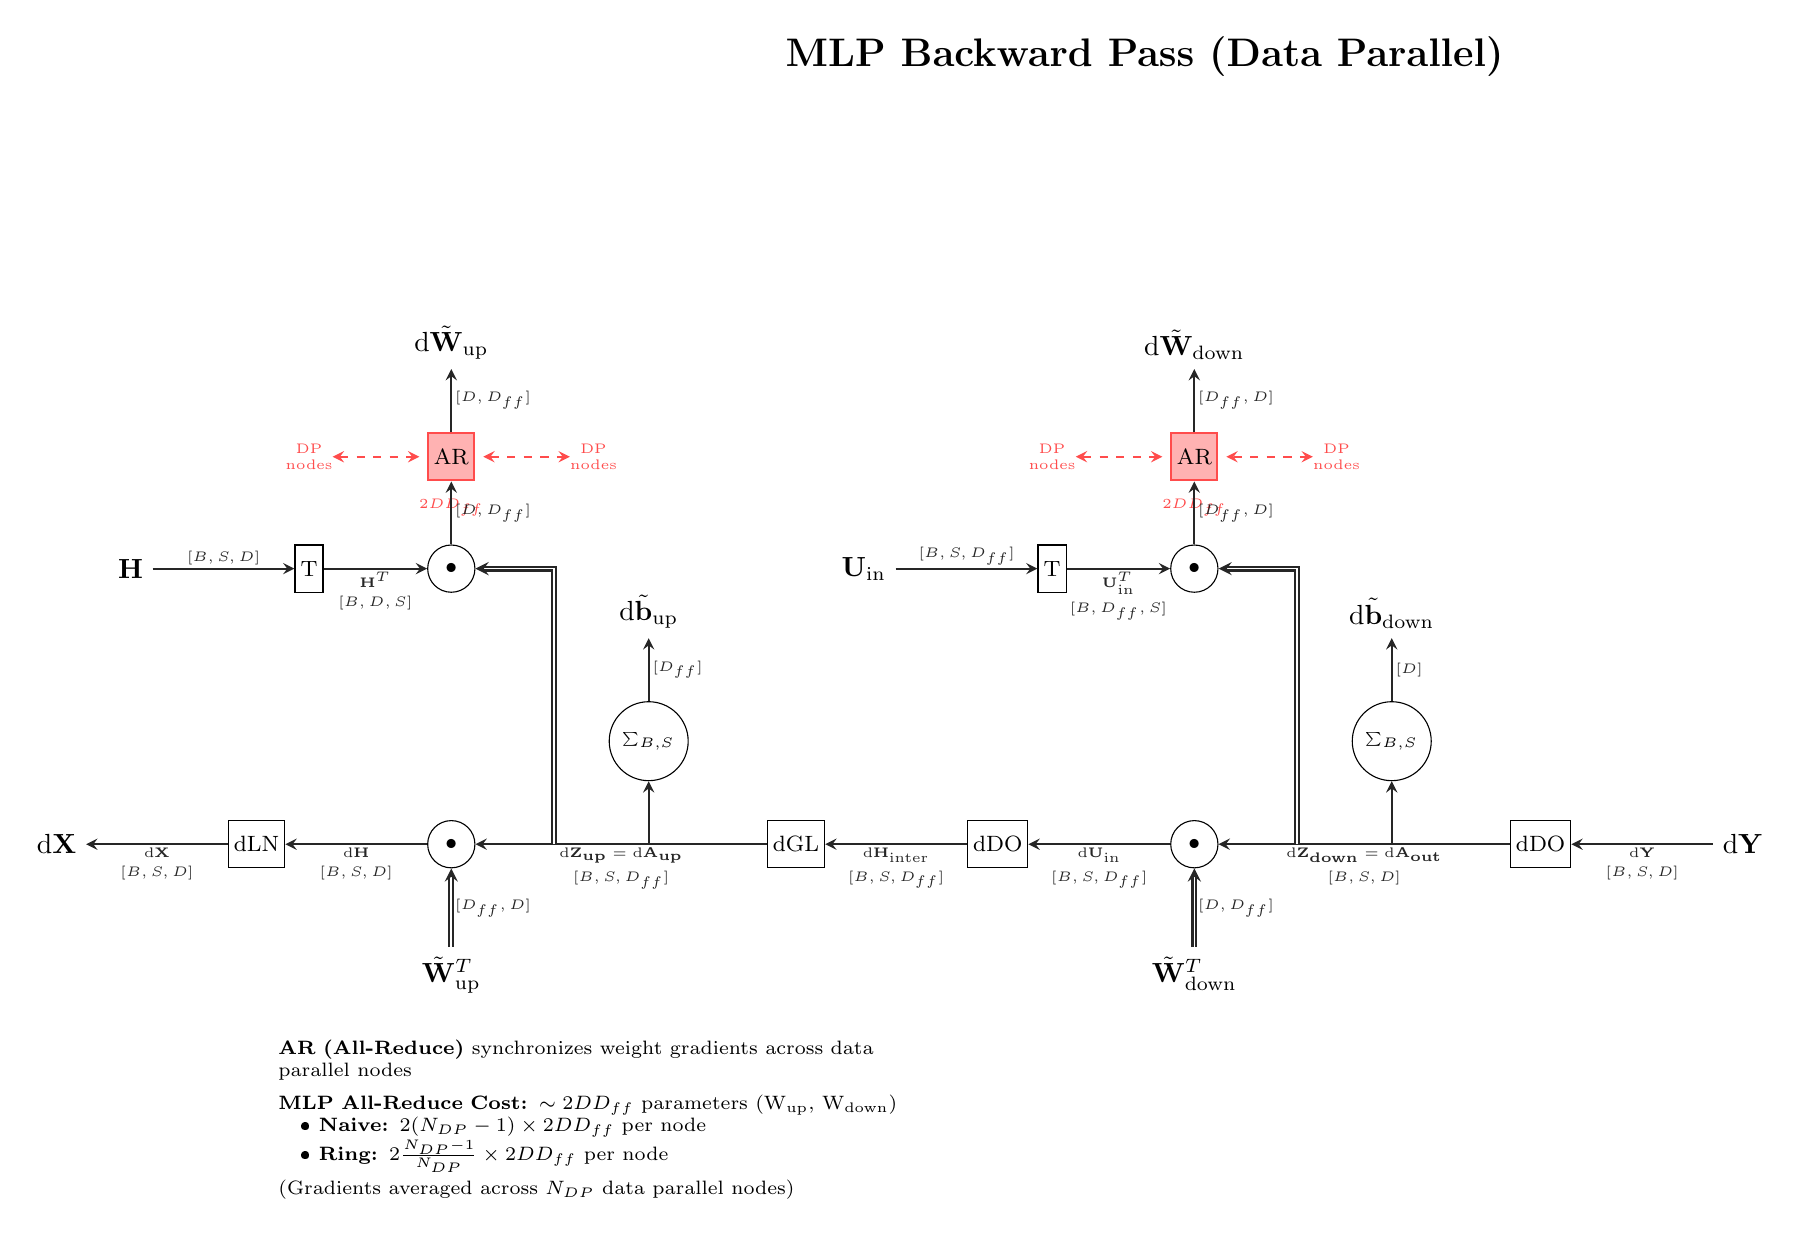
\begin{tikzpicture}[
    >=stealth,
    auxnode/.style={draw, rectangle, fill=white, minimum height=6mm, inner sep=2pt, font=\footnotesize, align=center},
    mulnode/.style={draw, circle, fill=white, minimum size=6mm, font=\footnotesize, align=center},
    addnode/.style={draw, circle, fill=white, minimum size=6mm, font=\footnotesize, align=center},
    sumnode/.style={draw, circle, fill=white, minimum size=6mm, font=\tiny, align=center},
    arnode/.style={draw, rectangle, fill=red!30, minimum height=6mm, inner sep=2pt, font=\footnotesize, align=center, thick, draw=red!70},
    flow_rev/.style={<-, thick, black!85},
    flow_dw/.style={->, thick, black!85},
    flow_act/.style={double, ->, thick, black!85},
    dimlabel/.style={font=\tiny, inner sep=1pt, align=center},
    gradlabel/.style={font=\tiny\bfseries, inner sep=1pt, align=center},
    dpgradweight/.style={->, thick, black!85},
    dpcomm/.style={<->, thick, red!70, dashed}
]
    \node[font=\Large\bfseries] at (5, 10) {MLP Backward Pass (Data Parallel)};

    \pgfmathsetmacro{\backwardoffset}{0.0}

    \node (d_MOut) at (12.6, \backwardoffset) {$\mathrm{d}\mathbf{Y}$};
    \node[auxnode] (d_Drop2) [left=1.8cm of d_MOut] {dDO};
    \draw[flow_rev] (d_Drop2) -- (d_MOut)
      node[dimlabel, midway, below]{\shortstack{$\mathrm{d}\mathbf{Y}$\\$[B,S,D]$}};

    \coordinate (split2) at ($(d_Drop2.west) + (-1.5cm, 0)$);
    \coordinate (branch_dUproj) at ($(split2) + (-1.2cm, 0)$);

    \node[sumnode] (d_SumB2) [above=0.8cm of split2] {$\sum_{B, S}$};
    \node (d_Bdown) [above=0.8cm of d_SumB2] {$\mathrm{d}\tilde{\mathbf{b}}_{\text{down}}$};
    \draw[dpgradweight] (d_SumB2) -- (d_Bdown) node[dimlabel, midway, right]{$[D]$};

    \draw[flow_rev] (d_SumB2) -- (split2);

    \node[mulnode] (d_L2Mul_in) [left=2.2cm of split2] {$\bullet$};
    \draw[flow_rev] (d_L2Mul_in) -- (d_Drop2)
      node[gradlabel, midway, below]{\shortstack{$\mathrm{d}\mathbf{Z}_{\text{down}}=\mathrm{d}\mathbf{A}_{\text{out}}$\\$[B,S,D]$}};

    \node (W_down_T) [below=1.0cm of d_L2Mul_in] {$\tilde{\mathbf{W}}_{\text{down}}^{T}$};
    \draw[flow_act] (W_down_T.north) -- (d_L2Mul_in)
      node[dimlabel, midway, right]{$[D, D_{ff}]$};

    \coordinate (L2Mul_w_y) at ($(d_L2Mul_in) + (0, 3.5cm)$);
    \node[mulnode] (d_L2Mul_w) at (L2Mul_w_y) {$\bullet$};

    % Add AR node before d_Wdown
    \node[arnode] (AR_down) [above=0.8cm of d_L2Mul_w] {AR};

    % Add communication arrows for AR_down
    \draw[dpcomm] ([xshift=-1.2cm]AR_down.west) -- ([xshift=-0.1cm]AR_down.west);
    \draw[dpcomm] ([xshift=0.1cm]AR_down.east) -- ([xshift=1.2cm]AR_down.east);
    \node[font=\tiny, red!70, align=center] at ([xshift=-1.5cm]AR_down.west) {DP\\nodes};
    \node[font=\tiny, red!70, align=center] at ([xshift=1.5cm]AR_down.east) {DP\\nodes};
    \node[font=\tiny, red!70, below=0.1cm of AR_down] {$2DD_{ff}$};

    \node (d_Wdown) [above=0.8cm of AR_down] {$\mathrm{d}\tilde{\mathbf{W}}_{\text{down}}$};
    \draw[dpgradweight] (d_L2Mul_w) -- (AR_down) node[dimlabel, midway, right]{$[D_{ff}, D]$};
    \draw[flow_dw] (AR_down) -- (d_Wdown) node[dimlabel, midway, right]{$[D_{ff}, D]$};

    \draw[flow_act] (branch_dUproj.north) |- (d_L2Mul_w.east);

    \node[auxnode] (Uin_T) at ($(d_L2Mul_w.west) + (-1.5cm, 0)$) {T};
    \draw[flow_dw] (Uin_T) -- (d_L2Mul_w)
      node[dimlabel, midway, below]{\shortstack{$\mathbf{U}_{\text{in}}^T$\\$[B, D_{ff}, S]$}};
    \node (Uin_aux) [left=1.8cm of Uin_T] {$\mathbf{U}_{\text{in}}$};
    \draw[flow_dw] (Uin_aux) -- (Uin_T) node[dimlabel, midway, above]{\shortstack{$[B,S,D_{ff}]$}};

    \node[auxnode] (d_Drop1) [left=1.8cm of d_L2Mul_in] {dDO};
    \draw[flow_rev] (d_Drop1) -- (d_L2Mul_in)
      node[dimlabel, midway, below]{\shortstack{$\mathrm{d}\mathbf{U}_{\text{in}}$\\$[B,S,D_{ff}]$}};

    \node[auxnode] (d_Act) [left=1.8cm of d_Drop1] {dGL};
    \draw[flow_rev] (d_Act) -- (d_Drop1)
      node[dimlabel, midway, below]{\shortstack{$\mathrm{d}\mathbf{H}_{\text{inter}}$\\$[B,S,D_{ff}]$}};

    \coordinate (split1) at ($(d_Act.west) + (-1.5cm, 0)$);
    \coordinate (branch_dHpre) at ($(split1) + (-1.2cm, 0)$);

    \node[sumnode] (d_SumB1) [above=0.8cm of split1] {$\sum_{B, S}$};
    \node (d_Bup) [above=0.8cm of d_SumB1] {$\mathrm{d}\tilde{\mathbf{b}}_{\text{up}}$};
    \draw[dpgradweight] (d_SumB1) -- (d_Bup) node[dimlabel, midway, right]{$[D_{ff}]$};

    \draw[flow_rev] (d_SumB1) -- (split1);

    \node[mulnode] (d_L1Mul_in) [left=2.2cm of split1] {$\bullet$};
    \draw[flow_rev] (d_L1Mul_in) -- (d_Act)
      node[gradlabel, midway, below]{\shortstack{$\mathrm{d}\mathbf{Z}_{\text{up}}=\mathrm{d}\mathbf{A}_{\text{up}}$\\$[B,S,D_{ff}]$}};

    \node (W_up_T) [below=1.0cm of d_L1Mul_in] {$\tilde{\mathbf{W}}_{\text{up}}^{T}$};
    \draw[flow_act] (W_up_T.north) -- (d_L1Mul_in)
      node[dimlabel, midway, right]{$[D_{ff}, D]$};

    \coordinate (L1Mul_w_y) at ($(d_L1Mul_in) + (0, 3.5cm)$);
    \node[mulnode] (d_L1Mul_w) at (L1Mul_w_y) {$\bullet$};

    % Add AR node before d_Wup
    \node[arnode] (AR_up) [above=0.8cm of d_L1Mul_w] {AR};

    % Add communication arrows for AR_up
    \draw[dpcomm] ([xshift=-1.2cm]AR_up.west) -- ([xshift=-0.1cm]AR_up.west);
    \draw[dpcomm] ([xshift=0.1cm]AR_up.east) -- ([xshift=1.2cm]AR_up.east);
    \node[font=\tiny, red!70, align=center] at ([xshift=-1.5cm]AR_up.west) {DP\\nodes};
    \node[font=\tiny, red!70, align=center] at ([xshift=1.5cm]AR_up.east) {DP\\nodes};
    \node[font=\tiny, red!70, below=0.1cm of AR_up] {$2DD_{ff}$};

    \node (d_Wup) [above=0.8cm of AR_up] {$\mathrm{d}\tilde{\mathbf{W}}_{\text{up}}$};
    \draw[dpgradweight] (d_L1Mul_w) -- (AR_up) node[dimlabel, midway, right]{$[D, D_{ff}]$};
    \draw[flow_dw] (AR_up) -- (d_Wup) node[dimlabel, midway, right]{$[D, D_{ff}]$};

    \draw[flow_act] (branch_dHpre.north) |- (d_L1Mul_w.east);

    \node[auxnode] (Znorm_T) at ($(d_L1Mul_w.west) + (-1.5cm, 0)$) {T};
    \draw[flow_dw] (Znorm_T) -- (d_L1Mul_w)
      node[dimlabel, midway, below]{\shortstack{$\mathbf{H}^T$\\$[B, D, S]$}};
    \node (Znorm_aux) [left=1.8cm of Znorm_T] {$\mathbf{H}$};
    \draw[flow_dw] (Znorm_aux) -- (Znorm_T) node[dimlabel, midway, above]{\shortstack{$[B,S,D]$}};

    \node[auxnode] (d_LN2) [left=1.8cm of d_L1Mul_in] {dLN};
    \draw[flow_rev] (d_LN2) -- (d_L1Mul_in)
      node[dimlabel, midway, below]{\shortstack{$\mathrm{d}\mathbf{H}$\\$[B,S,D]$}};

    \node (d_MIn) [left=1.8cm of d_LN2] {$\mathrm{d}\mathbf{X}$};
    \draw[flow_rev] (d_MIn) -- (d_LN2)
      node[dimlabel, midway, below]{\shortstack{$\mathrm{d}\mathbf{X}$\\$[B,S,D]$}};

    % Legend and explanation
    \node[align=left, font=\scriptsize, text width=8cm] at (-2, -3.5) {
      \textbf{AR (All-Reduce)} synchronizes weight gradients across data parallel nodes\\[4pt]
      \textbf{MLP All-Reduce Cost:} $\sim 2DD_{ff}$ parameters (W$_{\text{up}}$, W$_{\text{down}}$)\\
      \quad • \textbf{Naive:} $2(N_{DP}-1) \times 2DD_{ff}$ per node\\
      \quad • \textbf{Ring:} $2\frac{N_{DP}-1}{N_{DP}} \times 2DD_{ff}$ per node\\[2pt]
      {\scriptsize (Gradients averaged across $N_{DP}$ data parallel nodes)}
    };

\end{tikzpicture}%
}
  \caption{데이터 병렬 환경에서의 MLP 역전파.
  각 복제본은 자신의 미니배치를 사용해
  up-/down-projection 가중치와 bias에 대한 로컬 기울기를 계산한다.
  붉은 박스와 점선 화살표는 데이터 병렬 복제본 전체에 걸쳐
  이러한 기울기를 All-Reduce하여 전역 기울기를 형성하는 위치를 나타낸다.}
  \label{fig:mlp_backward_dp}
\end{figure}

% ------------------------ 7.5 Communication and Memory ----------------
\subsection{통신 및 메모리 고려사항}

마지막으로, 데이터 병렬화에서의 통신 비용과 메모리 요구사항을
단일 노드 모델과 비교해 보자.

\begin{itemize}
  \item \textbf{디바이스당 메모리.}
        각 디바이스는 모델 파라미터와 옵티마이저 상태의
        \emph{전체 복사본}을 저장한다.
        대신, 각 복제본이 보는 배치 크기가 $B_{\text{local}}$이므로,
        활성값(activation) 메모리는 대략 $N_D$배 감소한다.
  \item \textbf{통신 패턴.}
        데이터 병렬화가 도입하는 통신은
        파라미터 기울기를 동기화할 때의 All-Reduce뿐이다.
        순전파 경로나 활성값에 대해서는 통신이 없다.
  \item \textbf{확장성.}
        $N_D$를 늘리면 효과적인 배치 크기가 커지고,
        디바이스당 계산량과 활성 메모리는 줄어든다.
        반면, All-Reduce의 비용은 복제본 수와
        전체 파라미터 크기에 비례해 증가한다.
  \item \textbf{다른 병렬화 기법과의 결합.}
        실무에서는 데이터 병렬화가 텐서 병렬화(때로는 파이프라인 병렬화)와
        함께 사용되는 경우가 많다.
        이러한 설정에서는 각 데이터 병렬 그룹이
        여러 텐서 병렬 shard로 구성되며,
        기울기 동기화(All-Reduce)는 데이터 병렬 그룹 간에 수행되고,
        텐서 병렬 집합 통신은 각 그룹 내부에 국한된다.
\end{itemize}

Section~\ref{sec:sn}에서의 계산 그래프 관점에서 보면,
데이터 병렬화는 가장 “침습성이 낮은(least invasive)” 병렬화 방식이다.
레이어별 순전파·역전파 구조는 그대로 유지하면서,
그 위에 \emph{기울기 All-Reduce}만을 얹어놓는다고 볼 수 있다.

\else
  % ==========================================================
% 7. Data Parallelism (DP)
% ==========================================================
\section{Data Parallelism (DP)}
\label{sec:dp}

In data parallelism, each replica holds a full copy of the model, but
processes a different subset of the batch. Conceptually, each device runs
the same forward and backward computation as in the single-node setting
(Section~\ref{sec:sn}), but on a different mini-batch. After the backward pass,
gradients are synchronized across replicas via All-Reduce so that the
optimizer update is identical to what would have been obtained on a
single node with the full batch.

From the point of view of a single replica, the forward graph inside each
Transformer block is therefore identical to the one in
Section~\ref{sec:sn} (single-node), or to Section~\ref{sec:tp} (tensor-parallel) if TP is also
enabled. The only change is the input: instead of the full batch
$\mathbf{X} \in \mathbb{R}^{B \times S \times D}$, replica $d$ sees a
local shard $\mathbf{X}_d \in \mathbb{R}^{B_{\text{local}} \times S \times D}$,
with $B_{\text{local}} = B / N_D$.

We denote the number of data-parallel replicas by $N_D$. Devices are
indexed by $d \in \{0,\dots,N_D-1\}$.

\textbf{Key ideas:}
\begin{itemize}
  \item Each device has a full copy of the model parameters (weights and
        optimizer state).
  \item The global batch of size $B$ is split into $N_D$ local batches of
        size $B_{\text{local}} = B / N_D$.
  \item The forward pass on each device is identical to the single-node
        computation in Section~\ref{sec:sn}, but uses only its local batch.
  \item The backward pass computes local gradients
        $\nabla W^{(d)}$ on each device.
  \item All-Reduce over all data-parallel replicas averages or sums the
        gradients, producing the same effective update as a single-node
        run with batch size $B$.
\end{itemize}

In contrast to tensor parallelism (Section~\ref{sec:tp}), DP does not shard weight
matrices or activations; instead, it replicates the entire model and
splits only the data.

% ------------------------ 7.1 Overall DP Flow -------------------------
\subsection{Overall DP Training Flow}

Figure~\ref{fig:dp_overall_flow} shows a high-level view of data
parallelism applied to a Transformer layer. Compared to the single-node
overview (Figure~\ref{fig:single_node_overall}), the main difference is
that we now have $N_D$ identical copies of the block, each processing a
different input shard $\mathbf{X}_d$ and producing local predictions and
losses.

For a single training step, the sequence of operations is:

\begin{enumerate}
  \item \textbf{Batch sharding.} The input batch of size $B$ is split
        into $N_D$ local batches, each of size $B_{\text{local}}$:
        \[
          \{\mathbf{X}_0,\dots,\mathbf{X}_{N_D-1}\},
          \qquad
          \mathbf{X}_d \in \mathbb{R}^{B_{\text{local}} \times S \times D_{\text{in}}}.
        \]
        Each device $d$ also receives the corresponding target tokens
        $\mathbf{Y}_d$.
  \item \textbf{Local forward pass.} On each device, the full Transformer
        stack (input embedding, MHA, MLP, output projection) is applied to
        its local shard $\mathbf{X}_d$ exactly as in Section~\ref{sec:sn}. If tensor
        parallelism from Section~\ref{sec:tp} is also used, then each replica runs
        the same TP-augmented forward graph on $\mathbf{X}_d$. In either
        case, the structure of the forward pass is unchanged; only the
        batch dimension and the presence of gradient synchronization
        differ. Each device produces local logits, probabilities, and
        loss $\mathcal{L}_d$.
  \item \textbf{Local backward pass.} The loss $\mathcal{L}_d$ is
        backpropagated locally, yielding gradients
        $\nabla W^{(d)}$ for all parameters on device $d$.
  \item \textbf{Gradient synchronization (All-Reduce).} For each
        parameter tensor $W$, an All-Reduce over the data-parallel group
        is performed:
        \[
          \nabla W
            = \frac{1}{N_D}
              \sum_{d=0}^{N_D-1} \nabla W^{(d)}.
        \]
        After this step, all replicas hold identical averaged gradients
        $\nabla W$.
  \item \textbf{Optimizer update.} Each device applies the same optimizer
        (SGD, Adam, etc.) to its local copy of the parameters using the
        synchronized gradients. Because the gradients are identical across
        devices, the updated weights are also identical.
\end{enumerate}

Apart from the All-Reduce in step 4, the computations on each device are
identical copies of the single-node graph.

\begin{figure}[htbp]
  \centering
  \resizebox{\linewidth}{!}{%
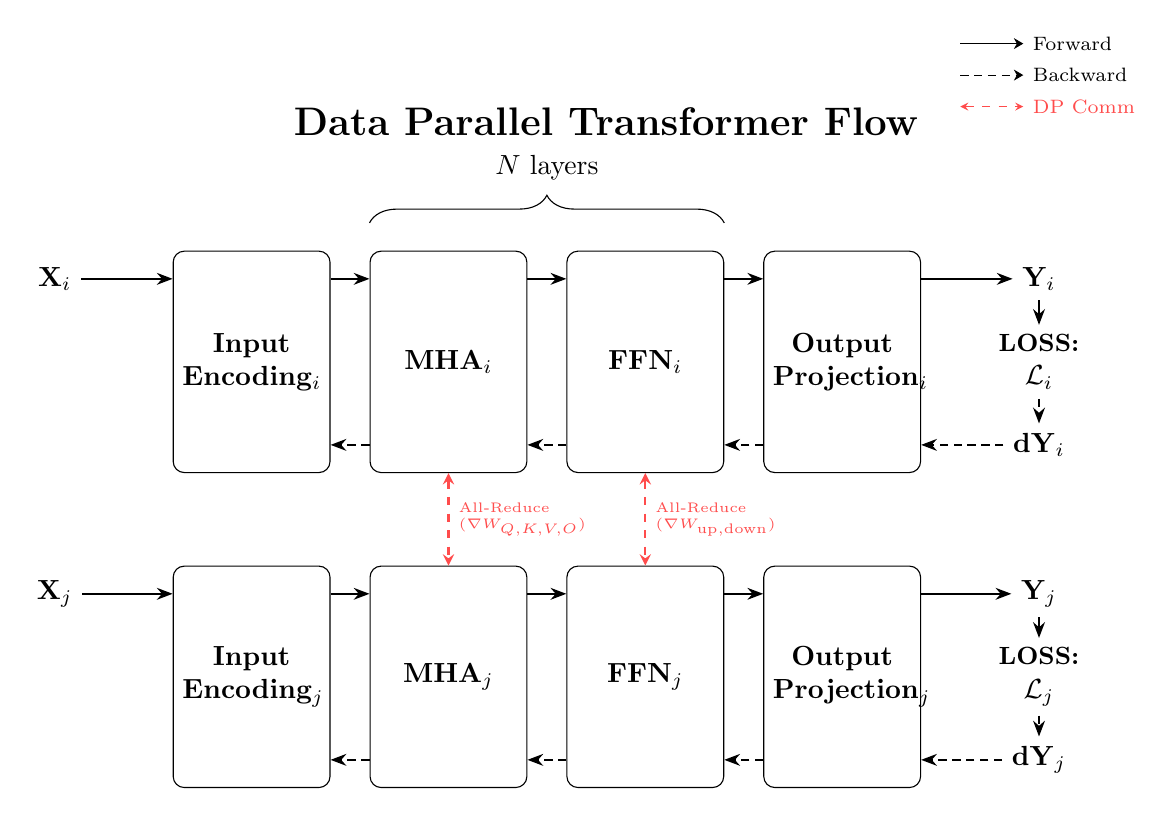
\begin{tikzpicture}[
    node distance=2.5cm,
    >=stealth,
    block/.style={rectangle, draw=black, fill=white, text width=5em, text centered, rounded corners, minimum height=8em, font=\bfseries},
    forward/.style={-{Stealth[length=2mm]}, thick, black},
    backward/.style={-{Stealth[length=2mm]}, thick, black, densely dashed},
    dpcomm/.style={<->, thick, red!70, dashed},
    io/.style={text centered, font=\bfseries}
]
    % Title
    \node[font=\Large\bfseries] at (7, 12) {Data Parallel Transformer Flow};

    % ========== Node i (Upper) ==========
    \node (input_i) [io] at (0, 10) {$\mathbf{X}_i$};
    \node (encoding_i) [block, right of=input_i, yshift=-3em] {Input\\Encoding$_i$};
    \node (mha_i) [block, right of=encoding_i] {MHA$_i$};
    \node (mlp_i) [block, right of=mha_i] {FFN$_i$};
    \node (output_i) [block, right of=mlp_i] {Output\\Projection$_i$};
    \node (pred_i) [io, right of=output_i, yshift=3em] {$\mathbf{Y}_i$};
    \node (loss_i) [align=center, io, right of=output_i] {\small LOSS:\\$\mathcal{L}_i$};
    \node (gradient_i) [io, right of=output_i, yshift=-3em] {$\mathbf{dY}_i$};

    % Forward arrows - Node i
    \draw [forward] (input_i) -- ([yshift=3em]encoding_i.west);
    \draw [forward] ([yshift=3em]encoding_i.east) -- ([yshift=3em]mha_i.west);
    \draw [forward] ([yshift=3em]mha_i.east) -- ([yshift=3em]mlp_i.west);
    \draw [forward] ([yshift=3em]mlp_i.east) -- ([yshift=3em]output_i.west);
    \draw [forward] ([yshift=3em]output_i.east) -- (pred_i);
    \draw [forward] (pred_i) -- (loss_i);
    \draw [backward] (loss_i) -- (gradient_i);

    % Backward arrows - Node i
    \draw [backward] (gradient_i) -- ([yshift=-3em]output_i.east);
    \draw [backward] ([yshift=-3em]output_i.west) -- ([yshift=-3em]mlp_i.east);
    \draw [backward] ([yshift=-3em]mlp_i.west) -- ([yshift=-3em]mha_i.east);
    \draw [backward] ([yshift=-3em]mha_i.west) -- ([yshift=-3em]encoding_i.east);

    % Brace for layer repetition - Node i
    \draw[decorate, decoration={brace, amplitude=10pt}]
        ([yshift=1.0em]mha_i.north west) -- ([yshift=1.0em]mlp_i.north east)
        node[midway, above=12pt, font=\normalsize] {$N$ layers};

    % ========== Node j (Lower) ==========
    \node (input_j) [io] at (0, 6) {$\mathbf{X}_j$};
    \node (encoding_j) [block, right of=input_j, yshift=-3em] {Input\\Encoding$_j$};
    \node (mha_j) [block, right of=encoding_j] {MHA$_j$};
    \node (mlp_j) [block, right of=mha_j] {FFN$_j$};
    \node (output_j) [block, right of=mlp_j] {Output\\Projection$_j$};
    \node (pred_j) [io, right of=output_j, yshift=3em] {$\mathbf{Y}_j$};
    \node (loss_j) [align=center, io, right of=output_j] {\small LOSS:\\$\mathcal{L}_j$};
    \node (gradient_j) [io, right of=output_j, yshift=-3em] {$\mathbf{dY}_j$};

    % Forward arrows - Node j
    \draw [forward] (input_j) -- ([yshift=3em]encoding_j.west);
    \draw [forward] ([yshift=3em]encoding_j.east) -- ([yshift=3em]mha_j.west);
    \draw [forward] ([yshift=3em]mha_j.east) -- ([yshift=3em]mlp_j.west);
    \draw [forward] ([yshift=3em]mlp_j.east) -- ([yshift=3em]output_j.west);
    \draw [forward] ([yshift=3em]output_j.east) -- (pred_j);
    \draw [forward] (pred_j) -- (loss_j);
    \draw [backward] (loss_j) -- (gradient_j);

    % Backward arrows - Node j
    \draw [backward] (gradient_j) -- ([yshift=-3em]output_j.east);
    \draw [backward] ([yshift=-3em]output_j.west) -- ([yshift=-3em]mlp_j.east);
    \draw [backward] ([yshift=-3em]mlp_j.west) -- ([yshift=-3em]mha_j.east);
    \draw [backward] ([yshift=-3em]mha_j.west) -- ([yshift=-3em]encoding_j.east);

    % ========== DP Communications ==========
    \draw [dpcomm] (mha_i.south) -- (mha_j.north) node[midway, right, font=\tiny, align=left] {All-Reduce\\$(\nabla W_{Q,K,V,O})$};
    \draw [dpcomm] (mlp_i.south) -- (mlp_j.north) node[midway, right, font=\tiny, align=left] {All-Reduce\\$(\nabla W_{\text{up},\text{down}})$};

    % Labels (Legend)
    \coordinate (legend) at ([xshift=11.5cm, yshift=8.5em]input_i);

    % Forward (작은 화살표 + 작은 글자)
    \draw[
        forward,
        -{Stealth[length=1.2mm,width=1.4mm]}, % 화살표 더 작게
        line width=0.3pt                       % 선 더 얇게
    ] (legend) -- ++(0.8,0)
      node[right, font=\scriptsize] {Forward};

    % Backward
    \draw[
        backward,
        -{Stealth[length=1.2mm,width=1.4mm]},
        line width=0.3pt
    ] ([yshift=-0.4cm]legend) -- ++(0.8,0)
      node[right, font=\scriptsize] {Backward};

    % DP Comm
    \draw[
        dpcomm,
        line width=0.3pt
    ] ([yshift=-0.8cm]legend) -- ++(0.8,0)
      node[right, font=\scriptsize] {DP Comm};
\end{tikzpicture}%
}
  \caption{Overall Transformer layer under data parallelism. Each device
  holds a full copy of the model and processes a different shard of the
  input batch ($\mathbf{X}_i$, $\mathbf{X}_j$, \dots). Forward and
  backward passes are performed locally as in the single-node case, and
  gradients for each block (MHA, MLP, output projection) are synchronized
  across replicas via All-Reduce.}
  \label{fig:dp_overall_flow}
\end{figure}


% ------------------------ 7.2 Relation to Single-Node -----------------
\subsection{Relationship to the Single-Node Computation}

It is often useful to think of DP as a pure “wrapper” around the
single-node computation from Section~\ref{sec:sn}:

\begin{itemize}
  \item \textbf{Same computation graph per replica.}
        For any given layer (MHA, MLP, output projection), the forward and
        backward graphs on a single device are identical to those in the
        single-node diagrams (Figures~\ref{fig:single_node_mha_forward},
        \ref{fig:single_node_mha_backward},
        \ref{fig:single_node_mlp_forward},
        \ref{fig:single_node_mlp_backward}, etc.), or to their
        tensor-parallel counterparts in Section~\ref{sec:tp} when TP is enabled.
        Only the input batch is different:
        $\mathbf{X}_d$ is a shard of the global batch.
  \item \textbf{Different mini-batches.}
        The only difference in the forward pass is that each replica sees
        a different chunk of the global batch. There is no communication
        needed for forward activations in DP.
  \item \textbf{Gradient aggregation only.}
        In the backward pass, each replica computes local gradients as if
        it were running independently. Only after all local gradients have
        been computed do we introduce communication: an All-Reduce over
        all replicas for each parameter tensor.
  \item \textbf{Equivalence to larger batch.}
        When gradients are averaged across replicas, the resulting update
        is mathematically equivalent to a single-node run with batch size
        $B = N_D \cdot B_{\text{local}}$ (ignoring subtle differences from
        e.g.\ dropout noise).
\end{itemize}

In contrast, tensor parallelism (Section~\ref{sec:tp}) changes the graph inside each
layer by sharding weight matrices and adding collectives in the middle of
the forward and backward passes. DP keeps the layer graphs intact and
adds communication only at the level of gradients.

% ------------------------ 7.3 MHA Backward under DP -------------------
\subsection{MHA Backward under DP}

For the multi-head attention block, the local backward pass on each device
is exactly the same as in
Figure~\ref{fig:single_node_mha_backward}: gradients flow from the loss
through the output projection, attention heads, Q/K/V projections, and
layer normalization back to the input $\mathbf{X}$.

The only DP-specific difference is how gradients with respect to the MHA
parameters are combined across replicas. Let
$W_Q, W_K, W_V, W_O$ be the query, key, value, and output projection
matrices. On device $d$, the local backward pass computes
$\nabla W_Q^{(d)}, \nabla W_K^{(d)}, \nabla W_V^{(d)}, \nabla W_O^{(d)}$.
An All-Reduce across all data-parallel replicas then aggregates these
gradients:
\[
  \nabla W_Q
    = \frac{1}{N_D} \sum_{d=0}^{N_D-1} \nabla W_Q^{(d)},\quad
  \nabla W_K
    = \frac{1}{N_D} \sum_{d=0}^{N_D-1} \nabla W_K^{(d)},
\]
\[
  \nabla W_V
    = \frac{1}{N_D} \sum_{d=0}^{N_D-1} \nabla W_V^{(d)},\quad
  \nabla W_O
    = \frac{1}{N_D} \sum_{d=0}^{N_D-1} \nabla W_O^{(d)}.
\]
After this synchronization, each device holds the same averaged gradients
$\nabla W_Q, \nabla W_K, \nabla W_V, \nabla W_O$.

Figure~\ref{fig:mha_backward_dp} illustrates this process: the internal
nodes and shapes inside the MHA block are identical to
Figure~\ref{fig:single_node_mha_backward}, but additional DP-specific
boxes and red dashed arrows mark the All-Reduce operations over replica
gradients.

\begin{landscape}
\begin{figure}[p]
  % no \centering here to avoid compilation issues
  \resizebox{\linewidth}{!}{%
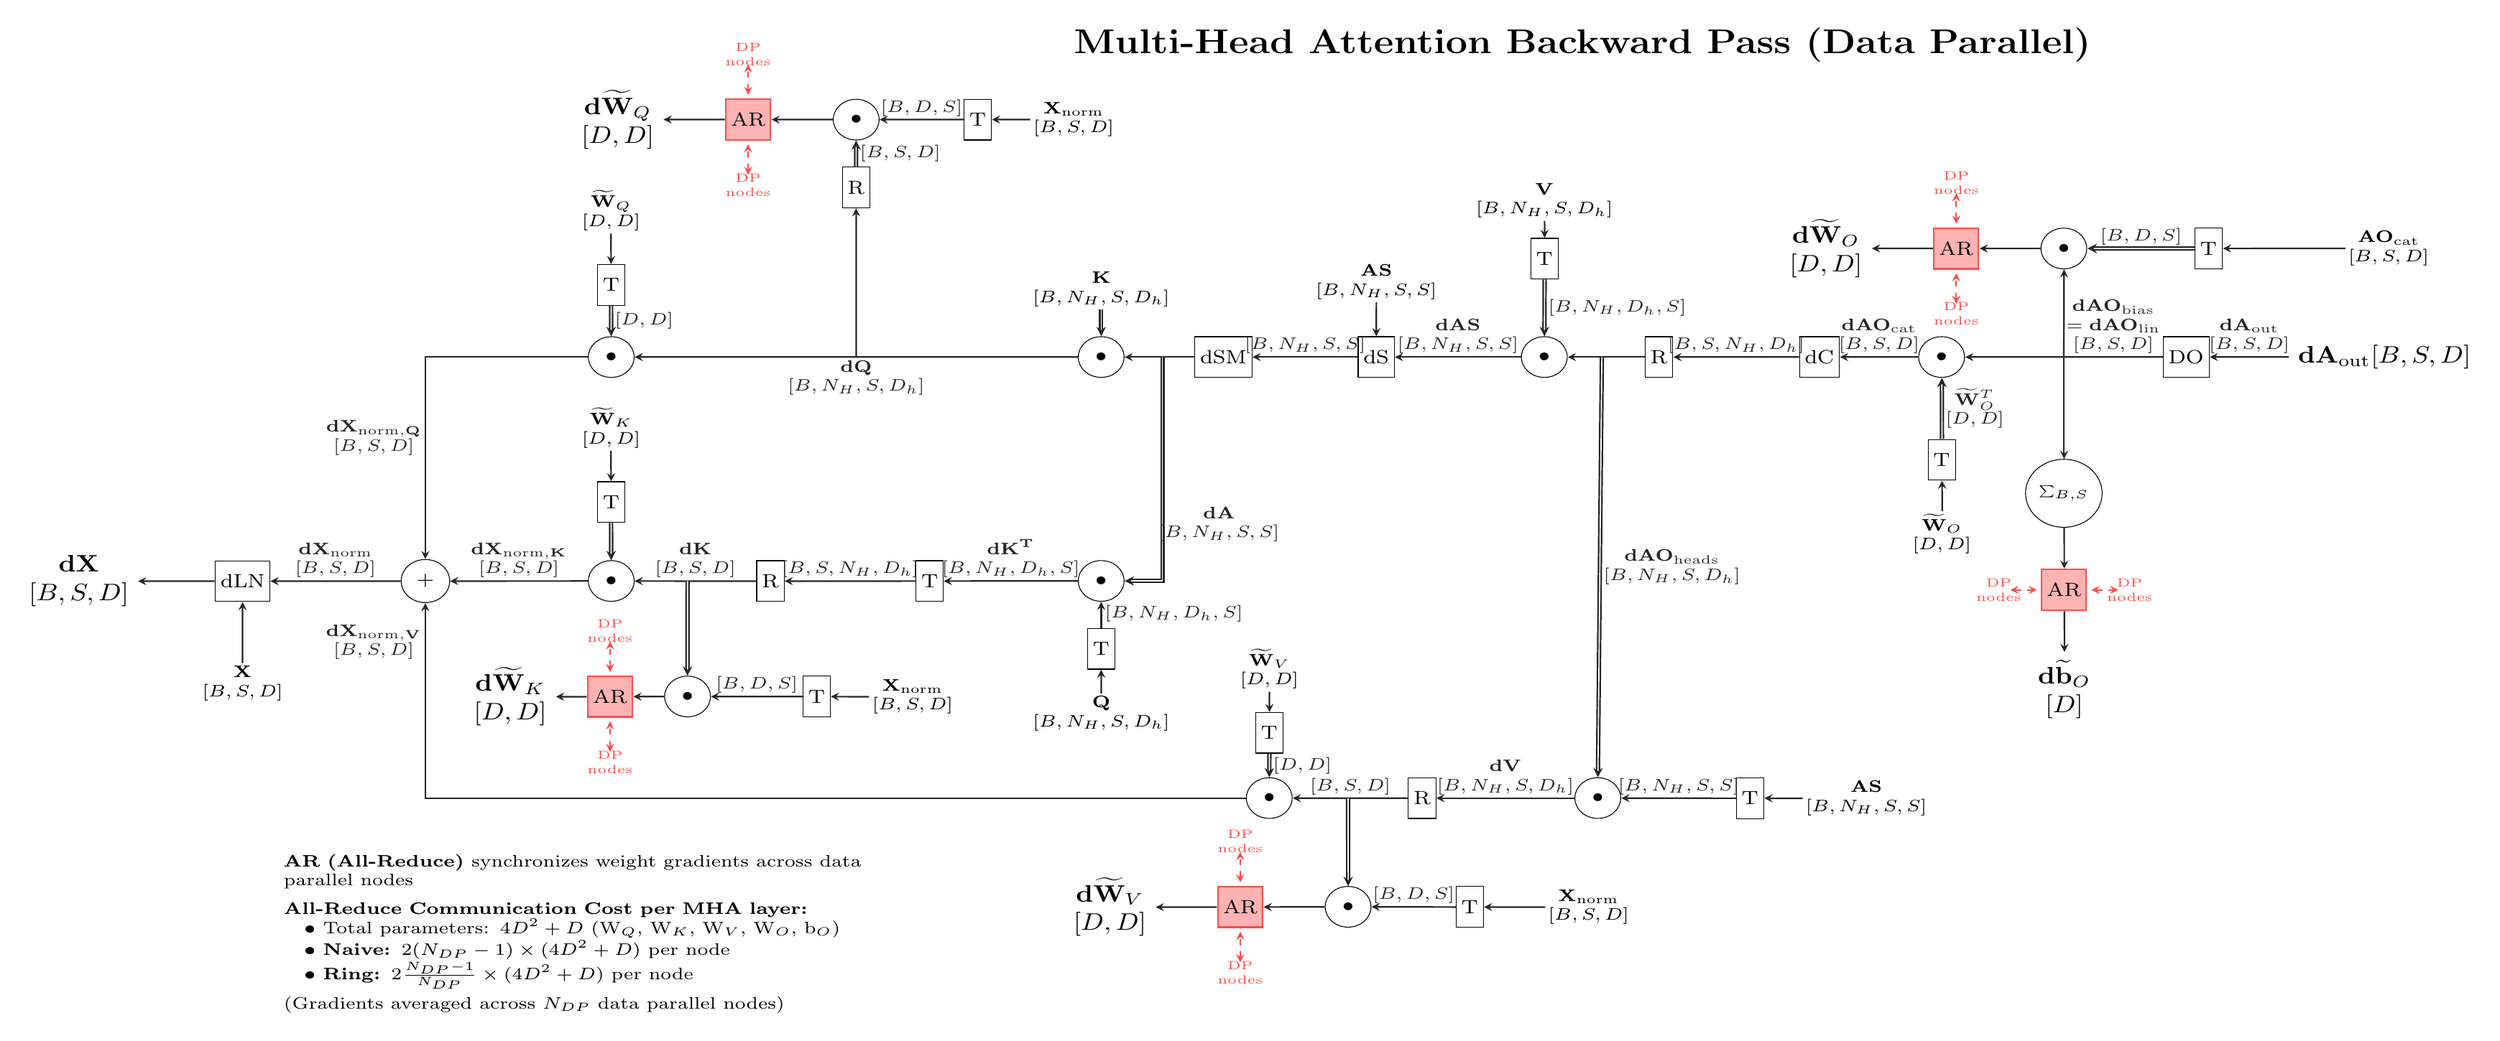
\begin{tikzpicture}[
  every node/.style={transform shape},
  >=stealth,
  auxnode/.style={draw, rectangle, fill=white, minimum height=6mm, inner sep=2pt, font=\footnotesize, align=center},
  mulnode/.style={draw, circle, fill=white, minimum size=6mm, font=\footnotesize, align=center},
  addnode/.style={draw, circle, fill=white, minimum size=6mm, font=\footnotesize, align=center},
  sumnode/.style={draw, circle, fill=white, minimum size=6mm, font=\tiny, align=center},
  arnode/.style={draw, rectangle, fill=red!30, minimum height=6mm, inner sep=2pt, font=\footnotesize, align=center, thick, draw=red!70},
  flow/.style={->, thick, black!85},
  flow2/.style={->, double, thick, black!85},
  dimlabel/.style={font=\scriptsize, inner sep=1pt, align=center},
  gradflow/.style={->, thick, black!85},
  gradweight/.style={->, thick, black!85},
  dpgradweight/.style={->, thick, black!85},
  dpcomm/.style={<->, thick, red!70, dashed}
]

\begin{scope}[xscale=1.35, yscale=1.2]

\def\yoffset{-1.0}
\def\dVXyoffset{-6.5}

\coordinate (Grad_Aout_B) at (17.5, \yoffset);
\coordinate (dDrop_center) at (15.9, \yoffset);
\coordinate (ProjGradSplit) at (14.3, \yoffset);
\coordinate (dOProj_center) at (12.7, \yoffset);
\coordinate (C_center) at (11.1, \yoffset);
\coordinate (R_center) at (9.0, \yoffset);
\coordinate (dPV_AS_calc_center) at (7.5, \yoffset);
\coordinate (dSoft_center) at (5.3, \yoffset);
\coordinate (dSM_calc_center) at (3.3, \yoffset);
\coordinate (dV_calc_center) at (8.2, \dVXyoffset+\yoffset);
\coordinate (R_V_bwd_center) at (5.9, \dVXyoffset+\yoffset);
\coordinate (dVX_calc_center) at (3.9, \dVXyoffset+\yoffset);
\coordinate (dQK_calc_Q_center) at (1.7, \yoffset);
\coordinate (dQK_calc_K_center) at (1.7, -3.3+\yoffset);
\coordinate (K_BWD_input_center) at (1.7, 1.0+\yoffset);
\coordinate (T_Q_bwd_center) at (1.7, -4.3+\yoffset);

\node[font=\Large\bfseries] at (8, 4.6+\yoffset) {Multi-Head Attention Backward Pass (Data Parallel)};

\node (Grad_Aout_B) at (18.5, \yoffset) {$\mathbf{dA}_{\text{out}}$\\$[B,S,D]$};
\node[auxnode] (DO) at (dDrop_center) {DO};
\node[mulnode] (dOProj) at (dOProj_center) {$\bullet$};

\node[auxnode] (T_WO) [below=0.9cm of dOProj] {T};
\node[dimlabel] (WO_BWD) [below=0.45cm of T_WO] {$\widetilde{\mathbf{W}}_{O}$\\$[D,D]$};

\node[mulnode] (dWO_calc) at ($(ProjGradSplit)+(0, 1.6)$) {$\bullet$};

% Add AR node before dWO
\node[arnode] (AR_WO) [left=0.8cm of dWO_calc] {AR};
\draw[dpcomm] ([yshift=-0.5cm]AR_WO.south) -- ([yshift=-0.05cm]AR_WO.south);
\draw[dpcomm] ([yshift=0.05cm]AR_WO.north) -- ([yshift=0.5cm]AR_WO.north);
\node[font=\tiny, red!70, align=center] at ([yshift=-0.65cm]AR_WO.south) {DP\\nodes};
\node[font=\tiny, red!70, align=center] at ([yshift=0.65cm]AR_WO.north) {DP\\nodes};

\node[align=center, left=0.8cm of AR_WO]
  (dWO_GRAD) {$\mathbf{d}\widetilde{\mathbf{W}}_{O}$\\$[D,D]$};
\draw[dpgradweight] (dWO_calc) -- (AR_WO);
\draw[gradflow] (AR_WO) -- (dWO_GRAD);

\node[auxnode] (T_AO_in) [right=1.4cm of dWO_calc] {T};
\node[dimlabel] (AO_in_local_label) [right=1.6cm of T_AO_in] {$\mathbf{AO}_{\text{cat}}$\\$[B,S,D]$};

\node[auxnode] (C) at (C_center) {dC};
\node[auxnode] (R) at (R_center) {R};

\node[mulnode] (dPV_AS_calc) at (dPV_AS_calc_center) {$\bullet$};
\node[auxnode] (dSoft) at (dSoft_center) {dS};
\node[auxnode] (dSM_calc) at (dSM_calc_center) {dSM};

\node[mulnode] (dQK_calc_Q) at (dQK_calc_Q_center) {$\bullet$};
\node[mulnode] (dQX_proj_calc) [left=5.8cm of dQK_calc_Q] {$\bullet$};

\node[mulnode] (dQK_calc_K) at (dQK_calc_K_center) {$\bullet$};
\node[mulnode] (dKX_proj_calc) [left=5.8cm of dQK_calc_K] {$\bullet$};

\node[dimlabel] (K_BWD_input) at (K_BWD_input_center) {$\mathbf{K}$\\$[B,N_H,S,D_h]$};
\node[auxnode] (T_Q_bwd) at (T_Q_bwd_center) {T};
\node[dimlabel] (Q_BWD_input) [below=0.35cm of T_Q_bwd] {$\mathbf{Q}$\\$[B,N_H,S,D_h]$};

\node[dimlabel] (V_FWD) [above=1.7cm of dPV_AS_calc] {$\mathbf{V}$\\$[B,N_H,S,D_h]$};
\node[auxnode] (T_V_bwd) [below=0.25cm of V_FWD] {T};

\node[mulnode] (dV_calc) at (dV_calc_center) {$\bullet$};
\node[auxnode] (T_AS_bwd) [right=1.5cm of dV_calc] {T};
\node[dimlabel] (AS_BWD_for_V) [right=0.5cm of T_AS_bwd] {$\mathbf{AS}$\\$[B,N_H,S,S]$};

\node[auxnode] (R_V_bwd) at (R_V_bwd_center) {R};
\node[mulnode] (dVX_calc) at (dVX_calc_center) {$\bullet$};

\node[auxnode] (T_WV) [above=0.35cm of dVX_calc] {T};
\node[dimlabel] (WV_BWD) [above=0.3cm of T_WV] {$\widetilde{\mathbf{W}}_{V}$\\$[D,D]$};

\node[sumnode] (Sum_dBO) [below=1.5cm of ProjGradSplit] {$\sum_{B, S}$};

% Add AR node before dBO
\node[arnode] (AR_BO) [below=0.6cm of Sum_dBO] {AR};
\draw[dpcomm] ([xshift=-0.4cm]AR_BO.west) -- ([xshift=-0.05cm]AR_BO.west);
\draw[dpcomm] ([xshift=0.05cm]AR_BO.east) -- ([xshift=0.4cm]AR_BO.east);
\node[font=\tiny, red!70, align=center] at ([xshift=-0.55cm]AR_BO.west) {DP\\nodes};
\node[font=\tiny, red!70, align=center] at ([xshift=0.55cm]AR_BO.east) {DP\\nodes};

\node[align=center] (dBO) [below=0.6cm of AR_BO] {$\mathbf{d}\widetilde{\mathbf{b}}_{O}$\\$[D]$};
\draw[dpgradweight] (Sum_dBO) -- (AR_BO);
\draw[gradflow] (AR_BO) -- (dBO);

\draw[gradflow] (Grad_Aout_B) -- (DO)
  node[dimlabel, midway, above]{$\mathbf{dA}_{\text{out}}$\\$[B,S,D]$};

\draw[gradflow] (DO) -- (dOProj)
  node[dimlabel, pos=0.25, above]{$\mathbf{dAO}_{\text{bias}}$\\$=\mathbf{dAO}_{\text{lin}}$\\$[B,S,D]$};

\draw[gradflow] (ProjGradSplit) -- (dWO_calc.south);
\draw[gradflow] (ProjGradSplit) -- ([yshift=-0.75cm]ProjGradSplit) -| (Sum_dBO.north);

\draw[gradflow] (dOProj) -- (C)
  node[dimlabel, midway, above]{$\mathbf{dAO}_{\text{cat}}$\\$[B,S,D]$};
\draw[gradflow] (C) -- (R)
  node[dimlabel, midway, above]{$[B,S,N_H,D_h]$};

\coordinate (R_split_point) at ($(dPV_AS_calc)!0.5!(R)$);
\draw[gradflow] (R.west) -- (dPV_AS_calc.east);
\draw[flow2] (R_split_point) -- (dV_calc.north)
  node[dimlabel, midway, right]{$\mathbf{dAO}_{\text{heads}}$\\$[B,N_H,S,D_h]$};

\draw[gradflow] (V_FWD.south) -- (T_V_bwd.north);
\draw[flow2] (T_V_bwd.south) -- (dPV_AS_calc.north)
  node[dimlabel, midway, right]{$[B,N_H,D_h,S]$};
\draw[gradflow] (dPV_AS_calc.west) -- (dSoft.east)
  node[dimlabel, midway, above]{$\mathbf{dAS}$\\$[B,N_H,S,S]$};

\node (AS_BWD_dS) [dimlabel, above=0.5cm of dSoft] {$\mathbf{AS}$\\$[B,N_H,S,S]$};
\draw[gradflow] (AS_BWD_dS.south) -- (dSoft.north);
\draw[gradflow] (dSoft.west) -- (dSM_calc.east)
  node[dimlabel, midway, above]{$[B,N_H,S,S]$};

\coordinate (dA_Split_X) at ($(dSM_calc_center)!0.5!(dQK_calc_Q_center)$);
\coordinate (dA_Split) at (dA_Split_X |- dQK_calc_Q.east);
\draw[gradflow] (dSM_calc.west) -- (dQK_calc_Q.east);
\draw[flow2] (dA_Split) -- (dA_Split |- dQK_calc_K.east) -- (dQK_calc_K.east)
  node[dimlabel, pos=-1.5, above, yshift=15]{$\mathbf{dA}$\\$[B,N_H,S,S]$};

\draw[flow2] (K_BWD_input.south) -- (dQK_calc_Q.north);
\draw[gradweight] (dQK_calc_Q) -- (dQX_proj_calc)
  node[dimlabel, midway, below]{$\mathbf{dQ}$\\$[B,N_H,S,D_h]$};

\node[auxnode] (T_WQ_bwd) [above=0.45cm of dQX_proj_calc] {T};
\node[dimlabel] (WQ_bwd) [above=0.45cm of T_WQ_bwd] {$\widetilde{\mathbf{W}}_{Q}$\\$[D,D]$};
\draw[flow] (WQ_bwd) -- (T_WQ_bwd);
\draw[flow2] (T_WQ_bwd.south) -- (dQX_proj_calc.north)
  node[dimlabel, midway, right]{$[D,D]$};

\draw[flow] (Q_BWD_input.north) -- (T_Q_bwd.south);
\draw[flow] (T_Q_bwd.north) -- (dQK_calc_K.south)
  node[dimlabel, pos=0.55, right]{$[B,N_H,D_h,S]$};

\node[auxnode] (T_dK) at ($(dQK_calc_K)!0.35!(dKX_proj_calc)$) {T};
\node[auxnode] (R_dK_mid) at ($(T_dK)!0.5!(dKX_proj_calc)$) {R};

\draw[gradweight] (dQK_calc_K) -- (T_dK)
  node[dimlabel, midway, above]{$\mathbf{dK^T}$\\$[B,N_H,D_h,S]$};
\draw[gradweight] (T_dK) -- (R_dK_mid)
  node[dimlabel, midway, above]{$[B,S,N_H,D_h]$};
\draw[gradweight] (R_dK_mid) -- (dKX_proj_calc)
  node[dimlabel, midway, above]{$\mathbf{dK}$\\$[B,S,D]$};

\node[auxnode] (T_WK_bwd) [above=0.55cm of dKX_proj_calc] {T};
\node[dimlabel] (WK_bwd) [above=0.45cm of T_WK_bwd] {$\widetilde{\mathbf{W}}_{K}$\\$[D,D]$};
\draw[gradflow] (WK_bwd) -- (T_WK_bwd);
\draw[flow2] (T_WK_bwd.south) -- (dKX_proj_calc.north);
\draw[gradflow] (AS_BWD_for_V.west) -- (T_AS_bwd.east);
\draw[gradflow] (T_AS_bwd.west) -- (dV_calc.east)
  node[dimlabel, midway, above]{$[B,N_H,S,S]$};
\draw[gradflow] (dV_calc.west) -- (R_V_bwd.east)
  node[dimlabel, midway, above]{$\mathbf{dV}$\\$[B,N_H,S,D_h]$};
\draw[gradflow] (R_V_bwd) -- (dVX_calc.east)
  node[dimlabel, midway, above]{$[B,S,D]$};

\draw[gradflow] (WV_BWD) -- (T_WV);
\draw[flow2] (T_WV) -- (dVX_calc.north)
  node[dimlabel, midway, right]{$[D,D]$};

\node[addnode] (Sum_dXnorm) [left=1.8cm of dKX_proj_calc] {$+$};

\draw[gradweight] (dQX_proj_calc.west) -| node[dimlabel, pos=0.7, left]{$\mathbf{dX}_{\text{norm},\mathbf{Q}}$\\$[B,S,D]$} (Sum_dXnorm.north);
\draw[gradweight] (dKX_proj_calc.west) -- node[dimlabel, midway, above]{$\mathbf{dX}_{\text{norm},\mathbf{K}}$\\$[B,S,D]$} (Sum_dXnorm.east);
\draw[gradweight] (dVX_calc.west) -| node[dimlabel, pos=0.9, left]{$\mathbf{dX}_{\text{norm},\mathbf{V}}$\\$[B,S,D]$} (Sum_dXnorm.south);

\coordinate (dV_branch) at ($(R_V_bwd.west)!0.52!(dVX_calc.east)$);
\node[mulnode] (dWV_mul) at ($(dV_branch)+(0,-1.6cm)$) {$\bullet$};
\draw[flow2] (dV_branch) -- (dWV_mul.north);

\node[auxnode] (T_Xnorm) [right=1.1cm of dWV_mul] {T};
\node[dimlabel] (Xnorm_local) [right=0.8cm of T_Xnorm] {$\mathbf{X}_{\text{norm}}$\\$[B,S,D]$};
\draw[gradflow] (Xnorm_local) -- (T_Xnorm);
\draw[gradflow] (T_Xnorm.west) -- (dWV_mul.east)
  node[dimlabel, midway, above]{$[B,D,S]$};

% Add AR node before dWV
\node[arnode] (AR_WV) [left=0.8cm of dWV_mul] {AR};
\draw[dpcomm] ([yshift=-0.5cm]AR_WV.south) -- ([yshift=-0.05cm]AR_WV.south);
\draw[dpcomm] ([yshift=0.05cm]AR_WV.north) -- ([yshift=0.5cm]AR_WV.north);
\node[font=\tiny, red!70, align=center] at ([yshift=-0.65cm]AR_WV.south) {DP\\nodes};
\node[font=\tiny, red!70, align=center] at ([yshift=0.65cm]AR_WV.north) {DP\\nodes};

\node[align=center] (dWV_out) [left=0.8cm of AR_WV] {$\mathbf{d}\widetilde{\mathbf{W}}_{V}$\\$[D,D]$};
\draw[dpgradweight] (dWV_mul.west) -- (AR_WV);
\draw[gradflow] (AR_WV) -- (dWV_out);

\coordinate (dQ_branch) at ($(dQK_calc_Q.east)!0.50!(dQX_proj_calc.west)$);
\node[mulnode] (dWQ_mul) at ($(dQ_branch)+(0,3.5cm)$) {$\bullet$};
\node[auxnode] (R_dQ_for_WQ) at ($(dWQ_mul)+(0,-1.0cm)$) {R};
\draw[gradflow]  (dQ_branch) -- (R_dQ_for_WQ.south);
\draw[flow2] (R_dQ_for_WQ.north) -- (dWQ_mul.south)
  node[dimlabel, midway, right]{$[B,S,D]$};

\node[auxnode] (T_XnormQ) [right=1.1cm of dWQ_mul] {T};
\node[dimlabel] (Xnorm_localQ) [right=0.5cm of T_XnormQ] {$\mathbf{X}_{\text{norm}}$\\$[B,S,D]$};
\draw[gradflow] (Xnorm_localQ) -- (T_XnormQ);
\draw[gradflow] (T_XnormQ.west) -- (dWQ_mul.east)
  node[dimlabel, midway, above]{$[B,D,S]$};

% Add AR node before dWQ
\node[arnode] (AR_WQ) [left=0.8cm of dWQ_mul] {AR};
\draw[dpcomm] ([yshift=-0.5cm]AR_WQ.south) -- ([yshift=-0.05cm]AR_WQ.south);
\draw[dpcomm] ([yshift=0.05cm]AR_WQ.north) -- ([yshift=0.5cm]AR_WQ.north);
\node[font=\tiny, red!70, align=center] at ([yshift=-0.65cm]AR_WQ.south) {DP\\nodes};
\node[font=\tiny, red!70, align=center] at ([yshift=0.65cm]AR_WQ.north) {DP\\nodes};

\node[align=center] (dWQ_out) [left=0.8cm of AR_WQ] {$\mathbf{d}\widetilde{\mathbf{W}}_{Q}$\\$[D,D]$};
\draw[dpgradweight] (dWQ_mul.west) -- (AR_WQ);
\draw[gradflow] (AR_WQ) -- (dWQ_out);

\coordinate (dK_branch) at ($(R_dK_mid)!0.52!(dKX_proj_calc)$);
\node[mulnode] (dWK_mul) at ($(dK_branch)+(0,-1.7cm)$) {$\bullet$};
\draw[flow2]  (dK_branch) -- (dWK_mul.north);

\node[auxnode] (T_XnormK) [right=1.2cm of dWK_mul] {T};
\node[dimlabel, right=0.5cm of T_XnormK] (Xnorm_localK) {$\mathbf{X}_{\text{norm}}$\\$[B,S,D]$};
\draw[gradflow] (Xnorm_localK) -- (T_XnormK);
\draw[gradflow] (T_XnormK.west) -- (dWK_mul.east)
  node[dimlabel, midway, above]{$[B,D,S]$};

% Add AR node before dWK
\node[arnode] (AR_WK) [left=0.4cm of dWK_mul] {AR};
\draw[dpcomm] ([yshift=-0.5cm]AR_WK.south) -- ([yshift=-0.05cm]AR_WK.south);
\draw[dpcomm] ([yshift=0.05cm]AR_WK.north) -- ([yshift=0.5cm]AR_WK.north);
\node[font=\tiny, red!70, align=center] at ([yshift=-0.65cm]AR_WK.south) {DP\\nodes};
\node[font=\tiny, red!70, align=center] at ([yshift=0.65cm]AR_WK.north) {DP\\nodes};

\node[align=center] (dWK_out) [left=0.4cm of AR_WK] {$\mathbf{d}\widetilde{\mathbf{W}}_{K}$\\$[D,D]$};
\draw[dpgradweight] (dWK_mul.west) -- (AR_WK);
\draw[gradflow] (AR_WK) -- (dWK_out);

\draw[gradflow] (WO_BWD) -- (T_WO);
\draw[flow2] (T_WO) -- (dOProj)
  node[dimlabel, midway, right]{$\widetilde{\mathbf{W}}_{O}^{T}$\\$[D,D]$};
\draw[gradflow] (AO_in_local_label) -- (T_AO_in);
\draw[flow2] (T_AO_in) -- (dWO_calc.east)
  node[dimlabel, midway, above]{$[B,D,S]$};

\node[auxnode] (dLN) [left=1.7cm of Sum_dXnorm] {dLN};
\draw[gradweight] (Sum_dXnorm.west) -- node[dimlabel, midway, above]
  {$\mathbf{dX}_{\text{norm}}$\\$[B,S,D]$} (dLN.east);

\node (dX_OUT) [align=center, left=1.0cm of dLN] {$\mathbf{dX}$\\$[B,S,D]$};
\draw[gradweight] (dLN.west) -- (dX_OUT);

\node[dimlabel] (LNCache) [below=0.9cm of dLN] {$\mathbf{X}$\\$[B,S,D]$};
\draw[gradflow] (LNCache.north) -- (dLN.south);

% Legend and explanation
    \node[align=left, font=\scriptsize, text width=8cm] at (-5, -9.5) {
      \textbf{AR (All-Reduce)} synchronizes weight gradients across data parallel nodes\\[4pt]
      \textbf{All-Reduce Communication Cost per MHA layer:}\\
      \quad • Total parameters: $4D^2 + D$ (W$_Q$, W$_K$, W$_V$, W$_O$, b$_O$)\\
      \quad • \textbf{Naive:} $2(N_{DP}-1) \times (4D^2 + D)$ per node\\
      \quad • \textbf{Ring:} $2\frac{N_{DP}-1}{N_{DP}} \times (4D^2 + D)$ per node\\[2pt]
      {\scriptsize (Gradients averaged across $N_{DP}$ data parallel nodes)}
    };

\end{scope}
\end{tikzpicture}
}
  \caption{Multi-head attention backward pass under data parallelism. Each
  replica computes local gradients w.r.t.\ $W_Q$, $W_K$, $W_V$, and $W_O$
  using its own mini-batch. Red dashed arrows indicate All-Reduce
  operations that aggregate these local gradients across all data-parallel
  replicas to form the global gradients used by the optimizer. The
  internal structure of the backward graph matches the single-node case.}
  \label{fig:mha_backward_dp}
\end{figure}
\end{landscape}

% ------------------------ 7.4 MLP Backward under DP -------------------
\subsection{MLP Backward under DP}

The situation for the MLP block is similar. Locally, each replica performs
exactly the same backward computations as in
Figure~\ref{fig:single_node_mlp_backward}: gradients propagate from
$\mathrm{d}\mathbf{Y}$ through the down-projection, activation,
up-projection, and (optional) layer normalization back to $\mathbf{H}$,
while accumulating parameter gradients for
$W_{\text{up}}, W_{\text{down}}, \mathbf{b}_{\text{up}},
\mathbf{b}_{\text{down}}$.

Under data parallelism, each replica $d$ obtains its own local gradients
$\nabla W_{\text{up}}^{(d)}, \nabla W_{\text{down}}^{(d)}$ and similarly
for the biases. These are then synchronized across replicas via
All-Reduce:
\[
  \nabla W_{\text{up}}
    = \frac{1}{N_D} \sum_{d=0}^{N_D-1} \nabla W_{\text{up}}^{(d)},\quad
  \nabla W_{\text{down}}
    = \frac{1}{N_D} \sum_{d=0}^{N_D-1} \nabla W_{\text{down}}^{(d)}.
\]
Bias gradients are treated analogously. Because the MLP input $\mathbf{H}$
is replicated across devices, no additional communication is needed for
$\mathrm{d}\mathbf{H}$ itself: each replica computes the same functional
backward map but with different data, and the effect of aggregation is
entirely captured by averaging the parameter gradients.

Figure~\ref{fig:mlp_backward_dp} marks the locations of these All-Reduce
operations in the MLP backward graph.

\begin{figure}[p]
  % no \centering here to avoid compilation issues
  \noindent
\resizebox{\linewidth}{!}{%
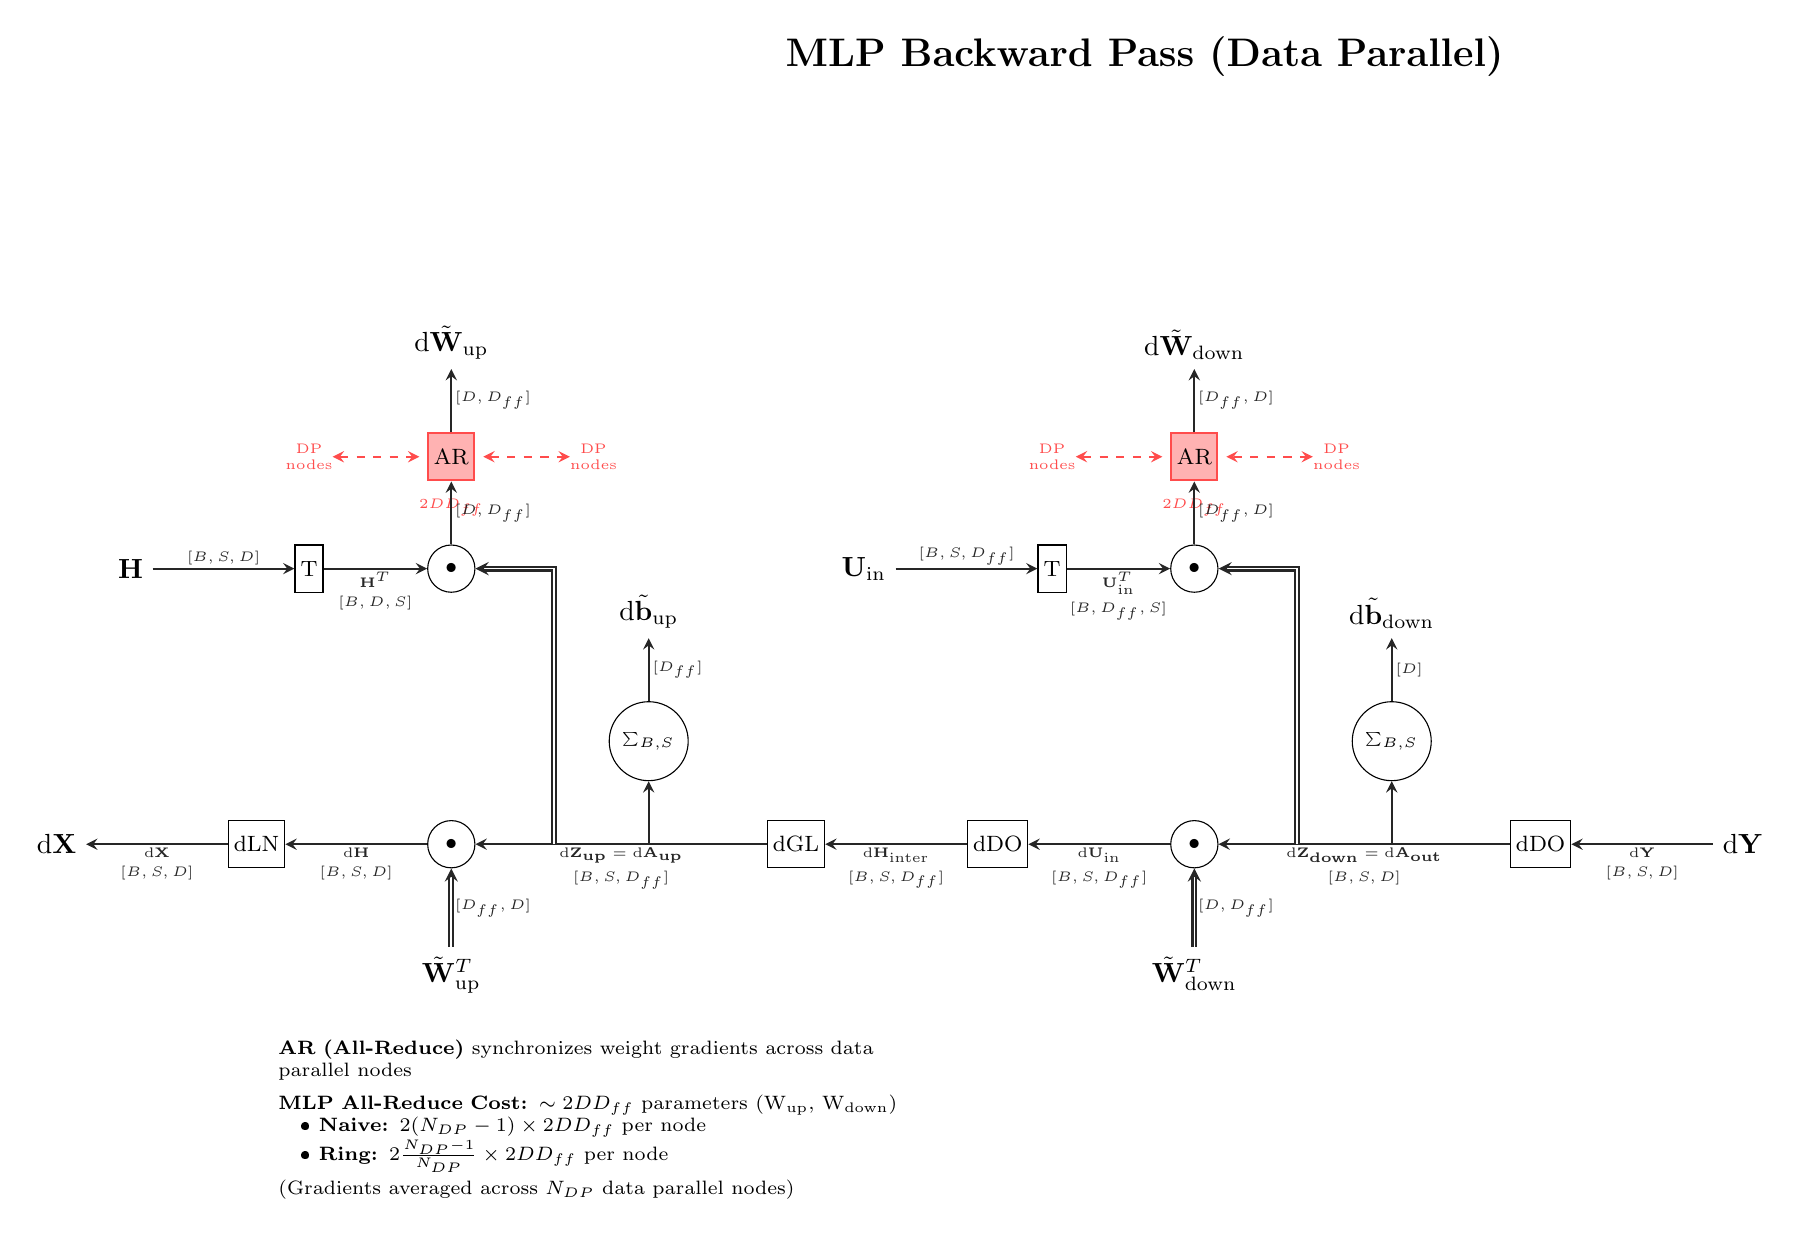
\begin{tikzpicture}[
    >=stealth,
    auxnode/.style={draw, rectangle, fill=white, minimum height=6mm, inner sep=2pt, font=\footnotesize, align=center},
    mulnode/.style={draw, circle, fill=white, minimum size=6mm, font=\footnotesize, align=center},
    addnode/.style={draw, circle, fill=white, minimum size=6mm, font=\footnotesize, align=center},
    sumnode/.style={draw, circle, fill=white, minimum size=6mm, font=\tiny, align=center},
    arnode/.style={draw, rectangle, fill=red!30, minimum height=6mm, inner sep=2pt, font=\footnotesize, align=center, thick, draw=red!70},
    flow_rev/.style={<-, thick, black!85},
    flow_dw/.style={->, thick, black!85},
    flow_act/.style={double, ->, thick, black!85},
    dimlabel/.style={font=\tiny, inner sep=1pt, align=center},
    gradlabel/.style={font=\tiny\bfseries, inner sep=1pt, align=center},
    dpgradweight/.style={->, thick, black!85},
    dpcomm/.style={<->, thick, red!70, dashed}
]
    \node[font=\Large\bfseries] at (5, 10) {MLP Backward Pass (Data Parallel)};

    \pgfmathsetmacro{\backwardoffset}{0.0}

    \node (d_MOut) at (12.6, \backwardoffset) {$\mathrm{d}\mathbf{Y}$};
    \node[auxnode] (d_Drop2) [left=1.8cm of d_MOut] {dDO};
    \draw[flow_rev] (d_Drop2) -- (d_MOut)
      node[dimlabel, midway, below]{\shortstack{$\mathrm{d}\mathbf{Y}$\\$[B,S,D]$}};

    \coordinate (split2) at ($(d_Drop2.west) + (-1.5cm, 0)$);
    \coordinate (branch_dUproj) at ($(split2) + (-1.2cm, 0)$);

    \node[sumnode] (d_SumB2) [above=0.8cm of split2] {$\sum_{B, S}$};
    \node (d_Bdown) [above=0.8cm of d_SumB2] {$\mathrm{d}\tilde{\mathbf{b}}_{\text{down}}$};
    \draw[dpgradweight] (d_SumB2) -- (d_Bdown) node[dimlabel, midway, right]{$[D]$};

    \draw[flow_rev] (d_SumB2) -- (split2);

    \node[mulnode] (d_L2Mul_in) [left=2.2cm of split2] {$\bullet$};
    \draw[flow_rev] (d_L2Mul_in) -- (d_Drop2)
      node[gradlabel, midway, below]{\shortstack{$\mathrm{d}\mathbf{Z}_{\text{down}}=\mathrm{d}\mathbf{A}_{\text{out}}$\\$[B,S,D]$}};

    \node (W_down_T) [below=1.0cm of d_L2Mul_in] {$\tilde{\mathbf{W}}_{\text{down}}^{T}$};
    \draw[flow_act] (W_down_T.north) -- (d_L2Mul_in)
      node[dimlabel, midway, right]{$[D, D_{ff}]$};

    \coordinate (L2Mul_w_y) at ($(d_L2Mul_in) + (0, 3.5cm)$);
    \node[mulnode] (d_L2Mul_w) at (L2Mul_w_y) {$\bullet$};

    % Add AR node before d_Wdown
    \node[arnode] (AR_down) [above=0.8cm of d_L2Mul_w] {AR};

    % Add communication arrows for AR_down
    \draw[dpcomm] ([xshift=-1.2cm]AR_down.west) -- ([xshift=-0.1cm]AR_down.west);
    \draw[dpcomm] ([xshift=0.1cm]AR_down.east) -- ([xshift=1.2cm]AR_down.east);
    \node[font=\tiny, red!70, align=center] at ([xshift=-1.5cm]AR_down.west) {DP\\nodes};
    \node[font=\tiny, red!70, align=center] at ([xshift=1.5cm]AR_down.east) {DP\\nodes};
    \node[font=\tiny, red!70, below=0.1cm of AR_down] {$2DD_{ff}$};

    \node (d_Wdown) [above=0.8cm of AR_down] {$\mathrm{d}\tilde{\mathbf{W}}_{\text{down}}$};
    \draw[dpgradweight] (d_L2Mul_w) -- (AR_down) node[dimlabel, midway, right]{$[D_{ff}, D]$};
    \draw[flow_dw] (AR_down) -- (d_Wdown) node[dimlabel, midway, right]{$[D_{ff}, D]$};

    \draw[flow_act] (branch_dUproj.north) |- (d_L2Mul_w.east);

    \node[auxnode] (Uin_T) at ($(d_L2Mul_w.west) + (-1.5cm, 0)$) {T};
    \draw[flow_dw] (Uin_T) -- (d_L2Mul_w)
      node[dimlabel, midway, below]{\shortstack{$\mathbf{U}_{\text{in}}^T$\\$[B, D_{ff}, S]$}};
    \node (Uin_aux) [left=1.8cm of Uin_T] {$\mathbf{U}_{\text{in}}$};
    \draw[flow_dw] (Uin_aux) -- (Uin_T) node[dimlabel, midway, above]{\shortstack{$[B,S,D_{ff}]$}};

    \node[auxnode] (d_Drop1) [left=1.8cm of d_L2Mul_in] {dDO};
    \draw[flow_rev] (d_Drop1) -- (d_L2Mul_in)
      node[dimlabel, midway, below]{\shortstack{$\mathrm{d}\mathbf{U}_{\text{in}}$\\$[B,S,D_{ff}]$}};

    \node[auxnode] (d_Act) [left=1.8cm of d_Drop1] {dGL};
    \draw[flow_rev] (d_Act) -- (d_Drop1)
      node[dimlabel, midway, below]{\shortstack{$\mathrm{d}\mathbf{H}_{\text{inter}}$\\$[B,S,D_{ff}]$}};

    \coordinate (split1) at ($(d_Act.west) + (-1.5cm, 0)$);
    \coordinate (branch_dHpre) at ($(split1) + (-1.2cm, 0)$);

    \node[sumnode] (d_SumB1) [above=0.8cm of split1] {$\sum_{B, S}$};
    \node (d_Bup) [above=0.8cm of d_SumB1] {$\mathrm{d}\tilde{\mathbf{b}}_{\text{up}}$};
    \draw[dpgradweight] (d_SumB1) -- (d_Bup) node[dimlabel, midway, right]{$[D_{ff}]$};

    \draw[flow_rev] (d_SumB1) -- (split1);

    \node[mulnode] (d_L1Mul_in) [left=2.2cm of split1] {$\bullet$};
    \draw[flow_rev] (d_L1Mul_in) -- (d_Act)
      node[gradlabel, midway, below]{\shortstack{$\mathrm{d}\mathbf{Z}_{\text{up}}=\mathrm{d}\mathbf{A}_{\text{up}}$\\$[B,S,D_{ff}]$}};

    \node (W_up_T) [below=1.0cm of d_L1Mul_in] {$\tilde{\mathbf{W}}_{\text{up}}^{T}$};
    \draw[flow_act] (W_up_T.north) -- (d_L1Mul_in)
      node[dimlabel, midway, right]{$[D_{ff}, D]$};

    \coordinate (L1Mul_w_y) at ($(d_L1Mul_in) + (0, 3.5cm)$);
    \node[mulnode] (d_L1Mul_w) at (L1Mul_w_y) {$\bullet$};

    % Add AR node before d_Wup
    \node[arnode] (AR_up) [above=0.8cm of d_L1Mul_w] {AR};

    % Add communication arrows for AR_up
    \draw[dpcomm] ([xshift=-1.2cm]AR_up.west) -- ([xshift=-0.1cm]AR_up.west);
    \draw[dpcomm] ([xshift=0.1cm]AR_up.east) -- ([xshift=1.2cm]AR_up.east);
    \node[font=\tiny, red!70, align=center] at ([xshift=-1.5cm]AR_up.west) {DP\\nodes};
    \node[font=\tiny, red!70, align=center] at ([xshift=1.5cm]AR_up.east) {DP\\nodes};
    \node[font=\tiny, red!70, below=0.1cm of AR_up] {$2DD_{ff}$};

    \node (d_Wup) [above=0.8cm of AR_up] {$\mathrm{d}\tilde{\mathbf{W}}_{\text{up}}$};
    \draw[dpgradweight] (d_L1Mul_w) -- (AR_up) node[dimlabel, midway, right]{$[D, D_{ff}]$};
    \draw[flow_dw] (AR_up) -- (d_Wup) node[dimlabel, midway, right]{$[D, D_{ff}]$};

    \draw[flow_act] (branch_dHpre.north) |- (d_L1Mul_w.east);

    \node[auxnode] (Znorm_T) at ($(d_L1Mul_w.west) + (-1.5cm, 0)$) {T};
    \draw[flow_dw] (Znorm_T) -- (d_L1Mul_w)
      node[dimlabel, midway, below]{\shortstack{$\mathbf{H}^T$\\$[B, D, S]$}};
    \node (Znorm_aux) [left=1.8cm of Znorm_T] {$\mathbf{H}$};
    \draw[flow_dw] (Znorm_aux) -- (Znorm_T) node[dimlabel, midway, above]{\shortstack{$[B,S,D]$}};

    \node[auxnode] (d_LN2) [left=1.8cm of d_L1Mul_in] {dLN};
    \draw[flow_rev] (d_LN2) -- (d_L1Mul_in)
      node[dimlabel, midway, below]{\shortstack{$\mathrm{d}\mathbf{H}$\\$[B,S,D]$}};

    \node (d_MIn) [left=1.8cm of d_LN2] {$\mathrm{d}\mathbf{X}$};
    \draw[flow_rev] (d_MIn) -- (d_LN2)
      node[dimlabel, midway, below]{\shortstack{$\mathrm{d}\mathbf{X}$\\$[B,S,D]$}};

    % Legend and explanation
    \node[align=left, font=\scriptsize, text width=8cm] at (-2, -3.5) {
      \textbf{AR (All-Reduce)} synchronizes weight gradients across data parallel nodes\\[4pt]
      \textbf{MLP All-Reduce Cost:} $\sim 2DD_{ff}$ parameters (W$_{\text{up}}$, W$_{\text{down}}$)\\
      \quad • \textbf{Naive:} $2(N_{DP}-1) \times 2DD_{ff}$ per node\\
      \quad • \textbf{Ring:} $2\frac{N_{DP}-1}{N_{DP}} \times 2DD_{ff}$ per node\\[2pt]
      {\scriptsize (Gradients averaged across $N_{DP}$ data parallel nodes)}
    };

\end{tikzpicture}%
}
  \caption{MLP backward pass under data parallelism. Each replica computes
  local gradients for the up- and down-projection weights and biases using
  its own mini-batch. Red boxes and dashed arrows indicate All-Reduce
  operations that aggregate these local parameter gradients across
  replicas. The structure of the backward computation inside each replica
  is identical to the single-node graph.}
  \label{fig:mlp_backward_dp}
\end{figure}


% ------------------------ 7.5 Communication and Memory ---------------
\subsection{Communication and Memory Considerations}

Compared to the single-node model in Section~\ref{sec:sn}:

\begin{itemize}
  \item \textbf{Memory per device.}
        Each device stores a full copy of the model parameters and
        optimizer states. Activation memory per device is reduced by a
        factor of $N_D$ because each replica sees only a fraction of the
        global batch.
  \item \textbf{Communication pattern.}
        DP introduces communication only at gradient synchronization time
        (All-Reduce over parameter gradients). There is no communication
        on the forward path and no communication for activations.
  \item \textbf{Scalability.}
        Increasing $N_D$ increases the effective batch size and reduces
        the per-device compute and activation memory, but the cost of
        All-Reduce grows with the number of replicas and the total
        parameter size.
  \item \textbf{Combination with other parallelism.}
        In practice, DP is often combined with tensor parallelism (and
        sometimes pipeline parallelism). In such settings, each data
        parallel group contains several tensor-parallel shards; gradient
        synchronization is then performed across data-parallel groups,
        while tensor-parallel collectives remain local to each group.
\end{itemize}

From the perspective of the computation graphs in Section~\ref{sec:sn}, data
parallelism is therefore the least invasive form of parallelism: it keeps
the per-layer forward and backward structure unchanged and adds only
gradient All-Reduces on top.

\fi
\clearpage

% ==========================================================
% 8. Hybrid Data + Tensor Parallelism (DP + TP)
% ==========================================================
\ifkorean
  % ==========================================================
% 8. 데이터 병렬화와 텐서 병렬화의 결합
% ==========================================================
\section{데이터 병렬화와 텐서 병렬화의 결합}
\label{sec:dp_tp}

앞 장들에서는 텐서 병렬화(TP, Section~\ref{sec:tp})와
데이터 병렬화(DP, Section~\ref{sec:dp})를 각각 따로 살펴보았다.
실제 대규모 학습 환경에서는 거의 항상 이 둘을 함께 사용한다.

\begin{itemize}
  \item \textbf{텐서 병렬화}는 큰 가중치 행렬과 활성값을
        \emph{모델 샤드(model shard)} 내부의 $N_T$개 디바이스에
        나누어 저장·계산한다.
  \item \textbf{데이터 병렬화}는 그 모델 샤드 전체를 $N_D$개 복제하여
        서로 다른 미니배치를 처리하고, 기울기를 동기화한다.
\end{itemize}

이 장의 목표는, 앞에서 정의한 단일 노드 및 TP/DP-only 계산 그래프 위에
DP+TP를 어떻게 “겹쳐서” 올려놓는지 개념적으로 정리하는 것이다.
즉, \emph{모델 차원 병렬화(TP)}와 \emph{배치 차원 병렬화(DP)}가
어떻게 직교하는지, 그리고 어디에서 집합 통신이 발생하는지를
시각적으로 이해할 수 있도록 하는 데 초점을 맞춘다.

% ------------------------ 8.1 Parallel Groups -------------------------
\subsection{병렬 그룹과 레이아웃}

우리는 전체 디바이스들을 개념적으로 2차원 격자 위에 배치한다.

\begin{itemize}
  \item \textbf{TP 축}: 각 행(row) 안의 $N_T$개 디바이스는
        하나의 텐서 병렬 그룹을 이루어 하나의 모델 샤드를 공동으로 저장한다.
  \item \textbf{DP 축}: 열(column) 방향으로는, 그 TP 그룹의
        $N_D$개 복제본이 서로 다른 배치 조각을 처리한다.
\end{itemize}

다르게 말하면 다음과 같다.

- 각 TP 그룹은 Section~\ref{sec:tp}의 “TP-only” 모델처럼 동작하지만,
  전체 배치가 아니라 \emph{로컬 배치 조각}만을 본다.
- 각 DP “열”은 Section~\ref{sec:dp}의 “DP-only” 설정과 비슷하지만,
  한 디바이스 대신 \emph{TP 그룹 전체}가 하나의 복제본 역할을 한다.

전역 배치 크기가 $B$라면, 이를 데이터 병렬 그룹에 대해
다음과 같이 나눈다.
\[
  B = N_D \cdot B_{\text{local}},
\]
따라서 DP 복제본 $d$는
$\mathbf{X}_d \in \mathbb{R}^{B_{\text{local}} \times S \times D}$를
입력으로 본다.
각 복제본 내부에서는 $\mathbf{X}_d$가
Section~\ref{sec:tp}에서와 동일한 TP-샤딩 모델로 들어간다:
단일 노드의 큰 matmul들은 $N_T$ 샤드에 걸친
컬럼/로우 병렬 쌍으로 대체된다.

Figure~\ref{fig:dp_tp_overall_flow}는 이러한 레이아웃을 요약한 그림이다.
이 그림은 단일 노드 개요(Figure~\ref{fig:single_node_overall})와
TP 개요(Figure~\ref{fig:tp_overall_flow})를
DP+TP 버전으로 확장한 것으로 읽으면 된다.

\begin{figure}[htbp]
  \centering
  \resizebox{\linewidth}{!}{%
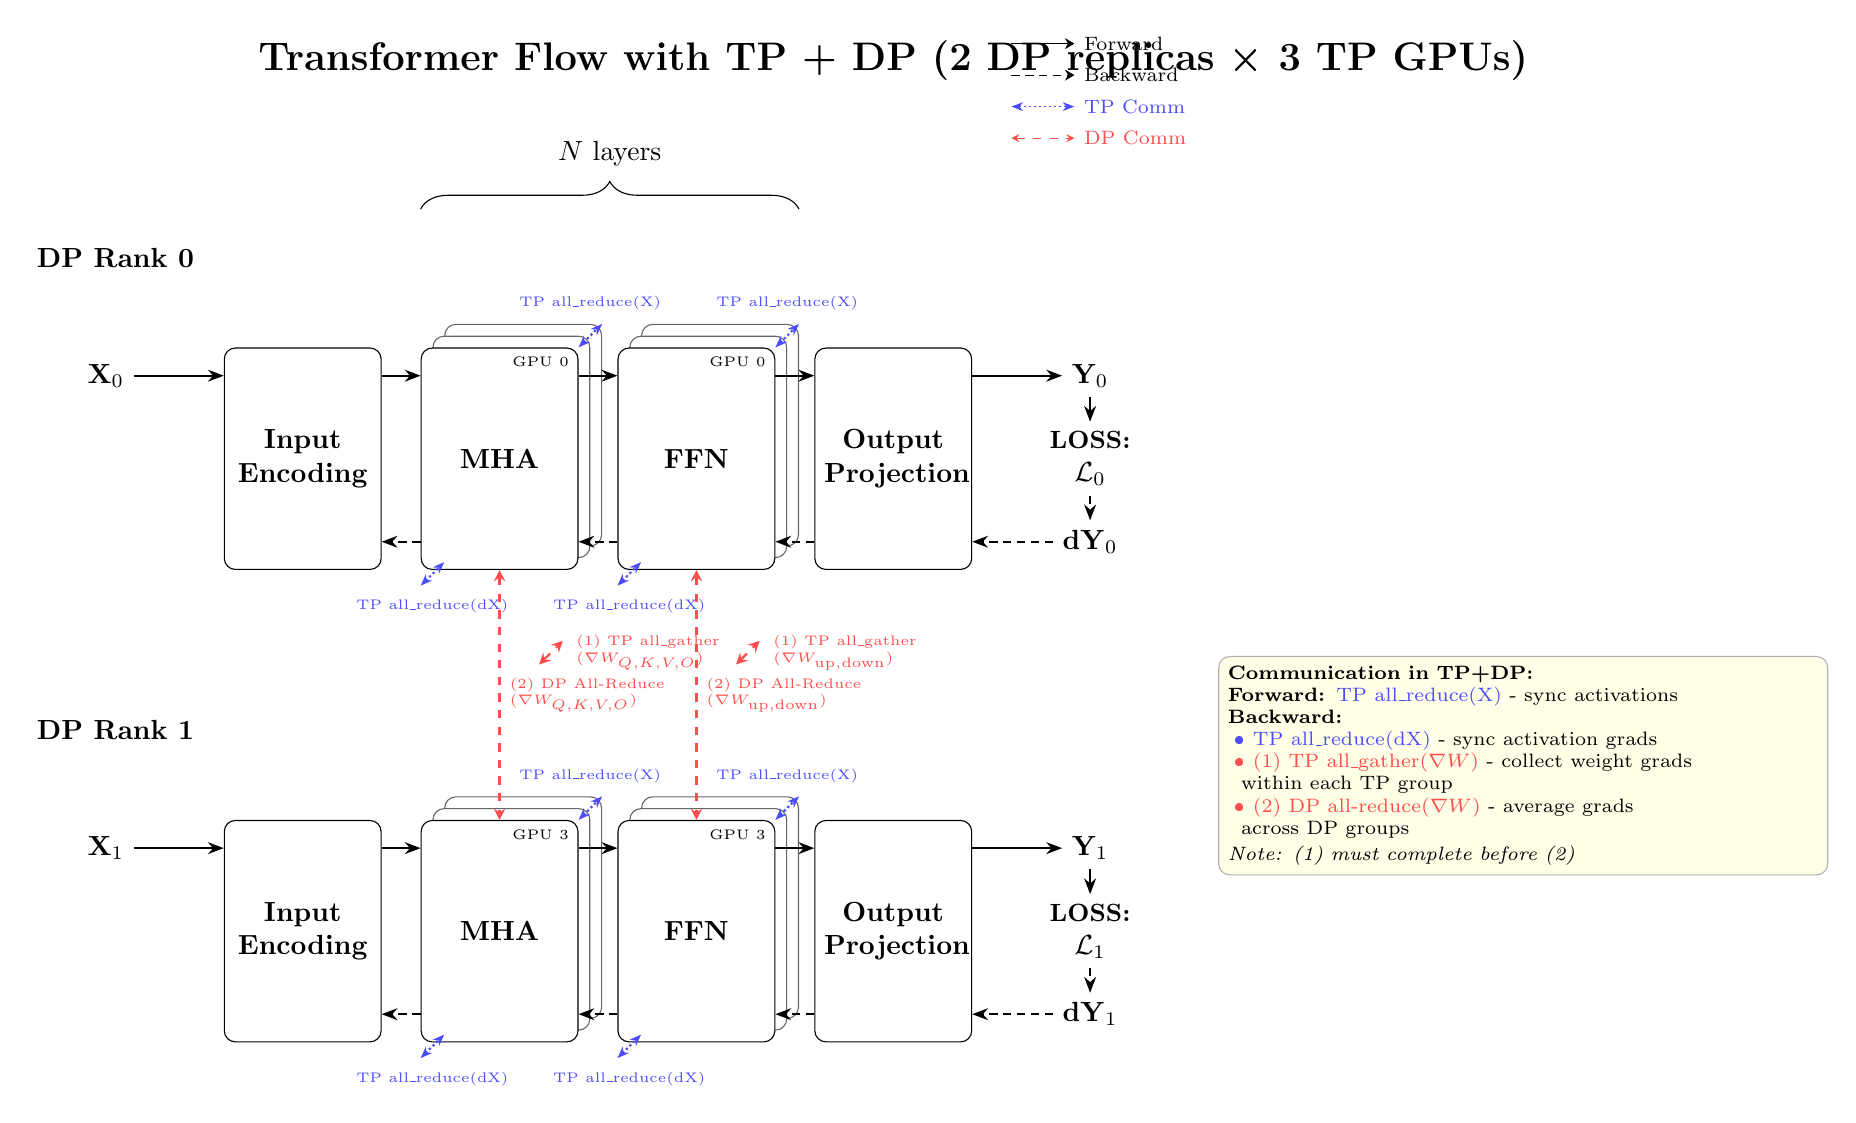
\begin{tikzpicture}[
    node distance=2.5cm,
    >=stealth,
    block/.style={rectangle, draw=black, fill=white, text width=5em, text centered, rounded corners, minimum height=8em, font=\bfseries},
    blockstack/.style={rectangle, draw=black!60, fill=white, text width=5em, text centered, rounded corners, minimum height=8em},
    forward/.style={-{Stealth[length=2mm]}, thick, black},
    backward/.style={-{Stealth[length=2mm]}, thick, black, densely dashed},
    tpcomm/.style={{Stealth[length=1.5mm]}-{Stealth[length=1.5mm]}, thick, blue!70, densely dotted},
    dpcomm/.style={<->, thick, red!70, dashed},
    io/.style={text centered, font=\bfseries}
]
    % Title
    \node[font=\Large\bfseries] at (10, 14) {Transformer Flow with TP + DP (2 DP replicas × 3 TP GPUs)};

    % ========== DP Replica 0 (Upper) ==========
    \node[font=\normalsize\bfseries, anchor=west] at (-1, 11.5) {DP Rank 0};

    \node (input_0) [io] at (0, 10) {$\mathbf{X}_0$};
    \node (encoding_0) [block, right of=input_0, yshift=-3em] {Input\\Encoding};

    % MHA blocks (3 stacked) - TP Group 0
    \node (mha3_0) [blockstack, right of=encoding_0, xshift=0.3cm, yshift=0.3cm] {};
    \node (mha2_0) [blockstack, right of=encoding_0, xshift=0.15cm, yshift=0.15cm] {};
    \node (mha_0) [block, right of=encoding_0] {MHA};
    \node[font=\tiny, anchor=north east] at (mha_0.north east) {GPU 0};

    % FFN blocks (3 stacked) - TP Group 0
    \node (mlp3_0) [blockstack, right of=mha_0, xshift=0.3cm, yshift=0.3cm] {};
    \node (mlp2_0) [blockstack, right of=mha_0, xshift=0.15cm, yshift=0.15cm] {};
    \node (mlp_0) [block, right of=mha_0] {FFN};
    \node[font=\tiny, anchor=north east] at (mlp_0.north east) {GPU 0};

    \node (output_0) [block, right of=mlp_0] {Output\\Projection};
    \node (pred_0) [io, right of=output_0, yshift=3em] {$\mathbf{Y}_0$};
    \node (loss_0) [align=center, io, right of=output_0] {\small LOSS:\\$\mathcal{L}_0$};
    \node (gradient_0) [io, right of=output_0, yshift=-3em] {$\mathbf{dY}_0$};

    % Forward arrows - DP Rank 0
    \draw [forward] (input_0) -- ([yshift=3em]encoding_0.west);
    \draw [forward] ([yshift=3em]encoding_0.east) -- ([yshift=3em]mha_0.west);
    \draw [forward] ([yshift=3em]mha_0.east) -- ([yshift=3em]mlp_0.west);
    \draw [forward] ([yshift=3em]mlp_0.east) -- ([yshift=3em]output_0.west);
    \draw [forward] ([yshift=3em]output_0.east) -- (pred_0);
    \draw [forward] (pred_0) -- (loss_0);
    \draw [backward] (loss_0) -- (gradient_0);

    % Backward arrows - DP Rank 0
    \draw [backward] (gradient_0) -- ([yshift=-3em]output_0.east);
    \draw [backward] ([yshift=-3em]output_0.west) -- ([yshift=-3em]mlp_0.east);
    \draw [backward] ([yshift=-3em]mlp_0.west) -- ([yshift=-3em]mha_0.east);
    \draw [backward] ([yshift=-3em]mha_0.west) -- ([yshift=-3em]encoding_0.east);

    % TP Communications - DP Rank 0
    % Forward All-Reduce
    \draw [tpcomm] (mha_0.north east) -- ([xshift=0.3cm, yshift=0.3cm]mha_0.north east);
    \node[font=\tiny, blue!70, anchor=south] at ([xshift=0.15cm, yshift=0.35cm]mha_0.north east) {TP all\_reduce(X)};

    \draw [tpcomm] (mlp_0.north east) -- ([xshift=0.3cm, yshift=0.3cm]mlp_0.north east);
    \node[font=\tiny, blue!70, anchor=south] at ([xshift=0.15cm, yshift=0.35cm]mlp_0.north east) {TP all\_reduce(X)};

    % Backward All-Reduce - dX
    \draw [tpcomm] ([yshift=-0.2cm]mlp_0.south west) -- ([xshift=0.3cm, yshift=0.1cm]mlp_0.south west);
    \node[font=\tiny, blue!70, anchor=north] at ([xshift=0.15cm, yshift=-0.25cm]mlp_0.south west) {TP all\_reduce(dX)};

    \draw [tpcomm] ([yshift=-0.2cm]mha_0.south west) -- ([xshift=0.3cm, yshift=0.1cm]mha_0.south west);
    \node[font=\tiny, blue!70, anchor=north] at ([xshift=0.15cm, yshift=-0.25cm]mha_0.south west) {TP all\_reduce(dX)};

    % Backward All-Gather for gradients - positioned on right side, before DP all-reduce
    \draw [dpcomm] ([xshift=-0.5cm, yshift=-1.2cm]mlp_0.south east) -- ([xshift=-0.2cm, yshift=-0.9cm]mlp_0.south east);
    \node[font=\tiny, red!70, anchor=west, align=left] at ([xshift=-0.15cm, yshift=-1.05cm]mlp_0.south east) {(1) TP all\_gather\\$(\nabla W_{\text{up},\text{down}})$};

    \draw [dpcomm] ([xshift=-0.5cm, yshift=-1.2cm]mha_0.south east) -- ([xshift=-0.2cm, yshift=-0.9cm]mha_0.south east);
    \node[font=\tiny, red!70, anchor=west, align=left] at ([xshift=-0.15cm, yshift=-1.05cm]mha_0.south east) {(1) TP all\_gather\\$(\nabla W_{Q,K,V,O})$};

    % Brace for layer repetition - DP Rank 0
    \draw[decorate, decoration={brace, amplitude=10pt}]
        ([yshift=5.0em]mha_0.north west) -- ([xshift=0.3cm, yshift=5.0em]mlp_0.north east)
        node[midway, above=12pt, font=\normalsize] {$N$ layers};

    % ========== DP Replica 1 (Lower) ==========
    \node[font=\normalsize\bfseries, anchor=west] at (-1, 5.5) {DP Rank 1};

    \node (input_1) [io] at (0, 4) {$\mathbf{X}_1$};
    \node (encoding_1) [block, right of=input_1, yshift=-3em] {Input\\Encoding};

    % MHA blocks (3 stacked) - TP Group 1
    \node (mha3_1) [blockstack, right of=encoding_1, xshift=0.3cm, yshift=0.3cm] {};
    \node (mha2_1) [blockstack, right of=encoding_1, xshift=0.15cm, yshift=0.15cm] {};
    \node (mha_1) [block, right of=encoding_1] {MHA};
    \node[font=\tiny, anchor=north east] at (mha_1.north east) {GPU 3};

    % FFN blocks (3 stacked) - TP Group 1
    \node (mlp3_1) [blockstack, right of=mha_1, xshift=0.3cm, yshift=0.3cm] {};
    \node (mlp2_1) [blockstack, right of=mha_1, xshift=0.15cm, yshift=0.15cm] {};
    \node (mlp_1) [block, right of=mha_1] {FFN};
    \node[font=\tiny, anchor=north east] at (mlp_1.north east) {GPU 3};

    \node (output_1) [block, right of=mlp_1] {Output\\Projection};
    \node (pred_1) [io, right of=output_1, yshift=3em] {$\mathbf{Y}_1$};
    \node (loss_1) [align=center, io, right of=output_1] {\small LOSS:\\$\mathcal{L}_1$};
    \node (gradient_1) [io, right of=output_1, yshift=-3em] {$\mathbf{dY}_1$};

    % Forward arrows - DP Rank 1
    \draw [forward] (input_1) -- ([yshift=3em]encoding_1.west);
    \draw [forward] ([yshift=3em]encoding_1.east) -- ([yshift=3em]mha_1.west);
    \draw [forward] ([yshift=3em]mha_1.east) -- ([yshift=3em]mlp_1.west);
    \draw [forward] ([yshift=3em]mlp_1.east) -- ([yshift=3em]output_1.west);
    \draw [forward] ([yshift=3em]output_1.east) -- (pred_1);
    \draw [forward] (pred_1) -- (loss_1);
    \draw [backward] (loss_1) -- (gradient_1);

    % Backward arrows - DP Rank 1
    \draw [backward] (gradient_1) -- ([yshift=-3em]output_1.east);
    \draw [backward] ([yshift=-3em]output_1.west) -- ([yshift=-3em]mlp_1.east);
    \draw [backward] ([yshift=-3em]mlp_1.west) -- ([yshift=-3em]mha_1.east);
    \draw [backward] ([yshift=-3em]mha_1.west) -- ([yshift=-3em]encoding_1.east);

    % TP Communications - DP Rank 1
    % Forward All-Reduce
    \draw [tpcomm] (mha_1.north east) -- ([xshift=0.3cm, yshift=0.3cm]mha_1.north east);
    \node[font=\tiny, blue!70, anchor=south] at ([xshift=0.15cm, yshift=0.35cm]mha_1.north east) {TP all\_reduce(X)};

    \draw [tpcomm] (mlp_1.north east) -- ([xshift=0.3cm, yshift=0.3cm]mlp_1.north east);
    \node[font=\tiny, blue!70, anchor=south] at ([xshift=0.15cm, yshift=0.35cm]mlp_1.north east) {TP all\_reduce(X)};

    % Backward All-Reduce - dX
    \draw [tpcomm] ([yshift=-0.2cm]mlp_1.south west) -- ([xshift=0.3cm, yshift=0.1cm]mlp_1.south west);
    \node[font=\tiny, blue!70, anchor=north] at ([xshift=0.15cm, yshift=-0.25cm]mlp_1.south west) {TP all\_reduce(dX)};

    \draw [tpcomm] ([yshift=-0.2cm]mha_1.south west) -- ([xshift=0.3cm, yshift=0.1cm]mha_1.south west);
    \node[font=\tiny, blue!70, anchor=north] at ([xshift=0.15cm, yshift=-0.25cm]mha_1.south west) {TP all\_reduce(dX)};

    % Backward All-Gather for gradients - positioned on right side, before DP all-reduce
    % \draw [dpcomm] ([xshift=0.5cm, yshift=-1.2cm]mlp_1.south east) -- ([xshift=0.8cm, yshift=-0.9cm]mlp_1.south east);
    % \node[font=\tiny, red!70, anchor=west, align=left] at ([xshift=0.85cm, yshift=-1.05cm]mlp_1.south east) {(1) TP all\_gather\\$(\nabla W_{\text{up},\text{down}})$};

    % \draw [dpcomm] ([xshift=0.5cm, yshift=-1.2cm]mha_1.south east) -- ([xshift=0.8cm, yshift=-0.9cm]mha_1.south east);
    % \node[font=\tiny, red!70, anchor=west, align=left] at ([xshift=0.85cm, yshift=-1.05cm]mha_1.south east) {(1) TP all\_gather\\$(\nabla W_{Q,K,V,O})$};

    % ========== DP Communications (Between TP Groups) ==========
    \draw [dpcomm] (mha_0.south) -- (mha_1.north) node[midway, right, font=\tiny, align=left, red!70] {(2) DP All-Reduce\\$(\nabla W_{Q,K,V,O})$};
    \draw [dpcomm] (mlp_0.south) -- (mlp_1.north) node[midway, right, font=\tiny, align=left, red!70] {(2) DP All-Reduce\\$(\nabla W_{\text{up},\text{down}})$};

    % Communication Order Annotation
    \node[font=\scriptsize, align=left, text width=7.5cm, draw=black!30, fill=yellow!10, rounded corners] at ([xshift=15.5cm, yshift=10em]encoding_1.south) {
        \textbf{Communication in TP+DP:}\\
        \textbf{Forward:} \textcolor{blue!70}{TP all\_reduce(X)} - sync activations\\
        \textbf{Backward:}\\
        \hspace{0.3em}\textcolor{blue!70}{• TP all\_reduce(dX)} - sync activation grads\\
        \hspace{0.3em}\textcolor{red!70}{• (1) TP all\_gather($\nabla W$)} - collect weight grads\\
        \hspace{0.6em}within each TP group\\
        \hspace{0.3em}\textcolor{red!70}{• (2) DP all-reduce($\nabla W$)} - average grads\\
        \hspace{0.6em}across DP groups\\[0.2em]
        \textit{Note: (1) must complete before (2)}
    };

    % Labels (Legend)
    \coordinate (legend) at ([xshift=11.5cm, yshift=12em]input_0);

    % Forward
    \draw[forward, -{Stealth[length=1.2mm,width=1.4mm]}, line width=0.3pt] (legend) -- ++(0.8,0)
      node[right, font=\scriptsize] {Forward};

    % Backward
    \draw[backward, -{Stealth[length=1.2mm,width=1.4mm]}, line width=0.3pt] ([yshift=-0.4cm]legend) -- ++(0.8,0)
      node[right, font=\scriptsize] {Backward};

    % TP Comm
    \draw[tpcomm, line width=0.3pt] ([yshift=-0.8cm]legend) -- ++(0.8,0)
      node[right, font=\scriptsize] {TP Comm};

    % DP Comm
    \draw[dpcomm, line width=0.3pt] ([yshift=-1.2cm]legend) -- ++(0.8,0)
      node[right, font=\scriptsize] {DP Comm};

\end{tikzpicture}%
}
  \caption{데이터 병렬화와 텐서 병렬화가 결합된 전체 트랜스포머 레이어.
  가로 방향으로는 각 텐서 병렬 그룹($N_T$ 디바이스)이
  하나의 샤딩된 레이어(Section~\ref{sec:tp})를 함께 구현한다.
  세로 방향으로는 그러한 그룹 $N_D$개가 데이터 병렬 격자를 이룬다.
  각 행은 서로 다른 미니배치 조각을 처리하며,
  기울기는 행들 사이에서 동기화된다.
  All-Reduce와 All-Gather 집합 통신이 사용되는 위치가
  그림에 함께 표시된다.}
  \label{fig:dp_tp_overall_flow}
\end{figure}

% ------------------------ 8.2 From Single-Node to TP to DP+TP --------
\subsection{단일 노드에서 텐서 병렬화, 그리고 데이터+텐서 병렬화까지}

DP+TP를 이해하는 한 가지 좋은 방법은,
Section~\ref{sec:sn}의 단일 노드 계산을 기준으로
\emph{점진적인 수정 단계}로 보는 것이다.

\paragraph{단일 노드 (Section~\ref{sec:sn}).}
모든 파라미터와 활성값이 하나의 디바이스에 있다.
각 선형 레이어는 하나의 matmul로 구현되며,
집합 통신은 전혀 필요 없다.

\paragraph{텐서 병렬화만 적용 (Section~\ref{sec:tp}).}
큰 행렬을 $N_T$ 디바이스에 나눈다.

\begin{itemize}
  \item \textbf{컬럼 병렬(linear)}:
        가중치를 출력 차원 방향으로 나눈다.
        각 샤드는 출력의 일부 슬라이스만 계산하고,
        이후 연산은 이 샤딩된 표현을 그대로 사용하거나,
        All-Gather를 통해 전체 텐서를 다시 조립한다.
  \item \textbf{로우 병렬(linear)}:
        가중치와 입력을 입력 차원 방향으로 나눈다.
        각 샤드는 부분 결과를 계산하고,
        All-Reduce로 부분 출력들을 합산한다.
\end{itemize}

하나의 TP 그룹 내부에서, 모든 디바이스는 같은 배치를 보며,
활성값은 피처 차원 방향으로 샤딩된다.
All-Reduce와 (필요하다면) All-Gather는
\emph{레이어 내부} 계산 그래프에 등장한다.

\paragraph{데이터 병렬화만 적용 (Section~\ref{sec:dp}).}
단일 노드 그래프는 그대로 두고, 이를 $N_D$ 디바이스에 복제한다.
각 디바이스는 서로 다른 미니배치 조각을 처리한다.
집합 통신은 역전파 끝에서 파라미터 기울기에 대해 수행하는
All-Reduce 한 번뿐이다.

\paragraph{데이터 병렬화와 텐서 병렬화를 결합.}
DP+TP에서는 위 두 가지 수정을 동시에 적용한다.

\begin{itemize}
  \item 각 데이터 병렬 복제본은 $N_T$ 디바이스로 구성된
        하나의 TP 그룹이다. 이 그룹 내부에서는
        Section~\ref{sec:tp}의 모든 TP 샤딩과 집합 통신이 그대로 적용된다.
  \item 데이터 병렬 복제본들 사이에서는
        Section~\ref{sec:dp}에서와 같이 기울기 All-Reduce를 수행하되,
        이제는 각 가중치 행렬의 \emph{TP 샤드}를 단위로 한다.
\end{itemize}

즉, 각 MHA/MLP/출력 블록의 \emph{샤드 단위} 내부 구조는
단일 TP-only 설정 때와 동일하고,
변하는 것은 “각 텐서에 몇 개의 디바이스가 관여하는지”와
“어떤 집합 통신이 어떤 디바이스를 잇는지”뿐이다.

% ------------------------ 8.3 Forward Pass under DP+TP ---------------
\subsection{데이터+텐서 병렬 환경에서의 순전파}

DP+TP 환경에서 한 TP 샤드가 보는 관점에서,
순전파는 기본적으로 TP-only 모델
(Section~\ref{sec:tp})과 같다.

\begin{itemize}
  \item 입력은 로컬 미니배치 조각
        $\mathbf{X}_d \in \mathbb{R}^{B_{\text{local}} \times S \times D}$이다.
  \item 컬럼 병렬 및 로우 병렬 선형 레이어가
        TP-only에서와 동일한 방식으로 적용된다.
  \item 중간 활성값(예: 헤드별 Q/K/V, MLP 중간 피처)은
        $N_T$ 디바이스에 샤딩된다.
\end{itemize}

여기에 \emph{추가}되는 것은, 어떤 이후 연산이
“샤딩되지 않은 전체 텐서”를 필요로 할 때
\textbf{활성값에 대한 All-Gather}를 사용하는 것이다.

대표적인 예시는 다음과 같다.

\begin{itemize}
  \item \textbf{어휘 병렬 출력 프로젝션.}
        최종 LM head 가중치 $\mathbf{W}_{\text{lm}}$이
        어휘 차원 방향으로 TP 디바이스에 샤딩되어 있다면,
        각 샤드는 어휘의 일부분에 대한 logits만 생성한다.
        전체 어휘에 대한 softmax/손실을 계산하려면,
        모든 샤드에서 나온 logits를 All-Gather로 모아
        크기가 $[B_{\text{local}}, S, V]$인 전체 텐서를
        구성해야 한다.
  \item \textbf{샤딩된 임베딩.}
        토큰 임베딩 행렬이 어휘 차원 방향으로 샤딩되어 있다면,
        임베딩 lookup 결과 역시 샤딩된 형태로 나온다.
        이후 레이어가 샤딩되지 않은
        $[B_{\text{local}}, S, D]$ 표현을 기대한다면,
        그 전에 All-Gather를 통해 임베딩을 합쳐줘야 한다.
  \item \textbf{샤딩되지 않은 연산들.}
        은닉 전체 차원에 작용하는 연산
        (예: 전역 정규화, 샤딩되지 않은 잔차 브랜치 등)은
        원칙적으로 전체 텐서를 필요로 하므로,
        그 전에 샤딩된 활성값을 All-Gather해야 할 수 있다.
        물론 모델을 설계할 때, 이러한 연산들이
        샤드 로컬로 동작하거나 TP 친화적인 변형으로 대체되도록
        구조를 잡으면, All-Gather를 줄일 수 있다.
\end{itemize}

정리하면, DP+TP 순전파에서 TP 그룹 내부의 All-Reduce/All-Gather 위치와
텐서 모양은 TP-only와 거의 같고,
데이터 병렬은 “어떤 미니배치 조각을 보느냐”만 바꾼다.
All-Gather 위치는 “샤딩된 텐서를 전역적으로 봐야 하는 연산”에 의해
결정된다.

% ------------------------ 8.4 Backward Pass and Gradient Sync --------
\subsection{데이터+텐서 병렬 환경에서의 역전파와 기울기 동기화}

DP+TP 환경에서 역전파는 다음 두 가지 요소를 결합한 것이다.

\begin{itemize}
  \item Section~\ref{sec:tp}에서의 TP-only 역전파 그래프
        (레이어 내부의 활성값/부분 기울기에 대한 All-Reduce와 All-Gather).
  \item Section~\ref{sec:dp}에서의 DP-only 기울기 동기화
        (이제는 각 TP 샤드 파라미터에 대해 적용).
\end{itemize}

특정 파라미터 텐서 $W$에 대해 보다 구체적으로 보면 다음과 같다.

\begin{itemize}
  \item \textbf{TP-only에서:}
    \begin{itemize}
      \item $W$는 TP 그룹 내부의 $N_T$ 디바이스에 대해
            $W^{(t)}$ 형태의 샤드로 나뉘어 저장된다
            ($t = 0,\dots,N_T-1$).
      \item 로컬 matmul 역전파를 통해 각 샤드에서
            로컬 기울기 $\nabla W^{(t)}$가 계산된다.
      \item $W$가 로우 병렬 구성에 등장한다면,
            입력에 대한 부분 기울기는 $t$에 대한 All-Reduce로 합쳐진다.
    \end{itemize}
  \item \textbf{DP+TP에서:}
    \begin{itemize}
      \item 위의 TP-only 로직이 각 데이터 병렬 복제본 $d$에 대해
            독립적으로 적용되어, 복제본 $d$의 샤드 $t$에 대해
            $\nabla W^{(t,d)}$를 얻는다.
      \item 그 다음, 각 샤드 $t$에 대해 복제본 인덱스 $d$에 대한
            All-Reduce를 수행한다:
            \[
              \nabla W^{(t)}
                = \frac{1}{N_D}
                  \sum_{d=0}^{N_D-1} \nabla W^{(t,d)}.
            \]
            이는 데이터 병렬 기울기 동기화이지만,
            이제 모든 TP 샤드에 대해 \emph{병렬로} 수행된다고 볼 수 있다.
    \end{itemize}
\end{itemize}

따라서 각 파라미터 샤드 $W^{(t)}$는 두 종류의 집합 통신에 참여한다.

\begin{itemize}
  \item \textbf{TP 그룹 내부 통신}:
        $t$에 대한 All-Reduce/All-Gather
        (로우/컬럼 병렬 로직에 따라).
  \item \textbf{DP 복제본 간 통신}:
        각 샤드 인덱스 $t$에 대해 $d$에 대한 All-Reduce
        (데이터 병렬 기울기 동기화).
\end{itemize}

이 조합 덕분에, 역전파가 끝났을 때
모든 DP 복제본의 모든 TP 그룹이
자신의 로컬 샤드 $W^{(t)}$에 대해
동일하고 올바르게 합산된 기울기를 가지게 되며,
전체 시스템에서 옵티마이저 업데이트가 일관되게 수행된다.

% ------------------------ 8.5 Communication Summary ------------------
\subsection{통신 요약 및 TP/DP 단독 설정과의 비교}

마지막으로, TP-only (Section~\ref{sec:tp}) 및 DP-only
(Section~\ref{sec:dp})와 비교했을 때
DP+TP의 주요 차이를 정리해 보자.

\paragraph{TP-only와 비교.}

\begin{itemize}
  \item \textbf{레이어별 샤딩 패턴은 동일.}
        하나의 TP 그룹 내부에서, 순전파/역전파 그래프 구조,
        All-Reduce/All-Gather의 위치, 텐서 모양은
        TP-only 설정과 완전히 동일하다.
  \item \textbf{DP 복제본 방향의 기울기 All-Reduce 추가.}
        각 파라미터 샤드는 이제 DP 축에 대해
        한 번 더 All-Reduce에 참여하여,
        서로 다른 미니배치 조각에서 온 기울기를 평균낸다.
  \item \textbf{로컬 활성값은 변하지 않음.}
        TP 그룹 내부의 활성 메모리 사용량과 계산 패턴은
        DP를 추가하더라도 변하지 않는다.
        DP는 각 복제본이 어떤 샘플을 보는지와,
        파라미터 기울기를 어떻게 합치는지만 바꾼다.
\end{itemize}

\paragraph{DP-only와 비교.}

\begin{itemize}
  \item \textbf{각 복제본 안의 샤딩된 모델.}
        DP-only에서는 각 복제본이 모델 전체를 그대로 가지고 있지만,
        DP+TP에서는 각 복제본이 TP-샤딩된 모델을 가진다.
        즉, 파라미터와 일부 활성값이 $N_T$ 디바이스에 나누어져 있다.
  \item \textbf{더 빈번한 집합 통신.}
        DP-only에서는 각 파라미터 텐서에 대해
        스텝당 한 번의 All-Reduce만 수행한다.
        반면 DP+TP에서는 여기에 더해,
        대부분의 레이어(MHA, MLP, 임베딩, LM head 등) 내부에
        TP 그룹 내부용 All-Reduce/All-Gather가 추가된다.
  \item \textbf{디바이스당 메모리·연산량.}
        TP는 디바이스당 파라미터·활성 메모리를
        대략 $1/N_T$만큼 줄여 주지만,
        그 대가로 레이어 내부 통신이 늘어난다.
        DP는 배치를 나누어 디바이스당 활성 메모리를
        추가로 $1/N_D$ 정도 줄여 준다.
\end{itemize}

전체적으로 DP+TP는 다음과 같이 이해할 수 있다.

\begin{quote}
  “Section~\ref{sec:tp}의 TP-샤딩된 트랜스포머 레이어를 가져와,
  Section~\ref{sec:dp}에서처럼 서로 다른 미니배치 조각에 대해 실행한 뒤,
  각 파라미터 샤드마다 복제본 간 기울기를 평균내기 위한
  All-Reduce를 하나 더 추가한다.”
\end{quote}

TP로 인해 샤딩된 활성값이 전역적으로 보여야 하는 곳
(예: 전체 어휘에 대한 logits)에서는 All-Gather가 사용되고,
뿐만 아니라 TP의 부분 결과를 합치거나
데이터 병렬 복제본 사이에서 기울기를 집계할 때는
All-Reduce가 사용된다.

\else
  % ==========================================================
% 8. Combining Data Parallelism (DP) and Tensor Parallelism (TP)
% ==========================================================
\section{Combining Data Parallelism (DP) and Tensor Parallelism (TP)}
\label{sec:dp_tp}

In previous sections we have treated tensor parallelism (TP, Section~\ref{sec:tp})
and data parallelism (DP, Section~\ref{sec:dp}) separately. In practice, large-scale
training almost always combines both:

\begin{itemize}
  \item \textbf{Tensor parallelism} splits large weight matrices and
        activations across $N_T$ devices inside a \emph{model shard}.
  \item \textbf{Data parallelism} replicates that model shard across
        $N_D$ different mini-batches and synchronizes gradients.
\end{itemize}

The total number of devices is therefore
\[
  N_{\text{devices}} = N_D \times N_T.
\]

From the point of view of the computation graph:

- Inside one TP group, the forward and backward graphs are identical to
  those in Section~\ref{sec:tp} (TP-only).
- Across DP replicas, the wrapping logic is identical to Section~\ref{sec:dp}
  (DP-only): each replica sees a different mini-batch and gradients are
  averaged across replicas.

The main difference from the previous chapters is therefore not in the
shape of the per-layer graphs, but in how devices are organized into
parallel groups and how multiple kinds of collective communication
(All-Reduce and All-Gather) interact.

% ------------------------ 8.1 Parallel Groups -------------------------
\subsection{Parallel Groups and Layout}

We conceptually arrange devices into a 2D grid:

\begin{itemize}
  \item \textbf{TP dimension}: within each row, $N_T$ devices form a
        tensor-parallel group and jointly store a single model shard.
  \item \textbf{DP dimension}: along the column dimension, $N_D$ copies of
        that TP group process different shards of the batch.
\end{itemize}

In other words:

- Each TP group behaves like the TP-only model of Section~\ref{sec:tp}, but only sees
  a local shard of the batch.
- Each DP “column” behaves like the DP-only setup of Section~\ref{sec:dp}, but each
  replica is itself a TP group instead of a single device.

If the global batch has size $B$, we split it across data-parallel groups
as
\[
  B = N_D \cdot B_{\text{local}},
\]
so that DP replica $d$ sees $\mathbf{X}_d \in \mathbb{R}^{B_{\text{local}}
\times S \times D}$ as its input. Within each replica, $\mathbf{X}_d$ is
fed into the TP-sharded model exactly as in Section~\ref{sec:tp}: single-node
matmuls are replaced by column-parallel / row-parallel pairs across the
$N_T$ shards.

Figure~\ref{fig:dp_tp_overall_flow} summarizes this layout and should be
read as a DP+TP version of the single-node overview from
Figure~\ref{fig:single_node_overall} and the TP overview in
Figure~\ref{fig:tp_overall_flow}.

\begin{figure}[htbp]
  \centering
  \resizebox{\linewidth}{!}{%
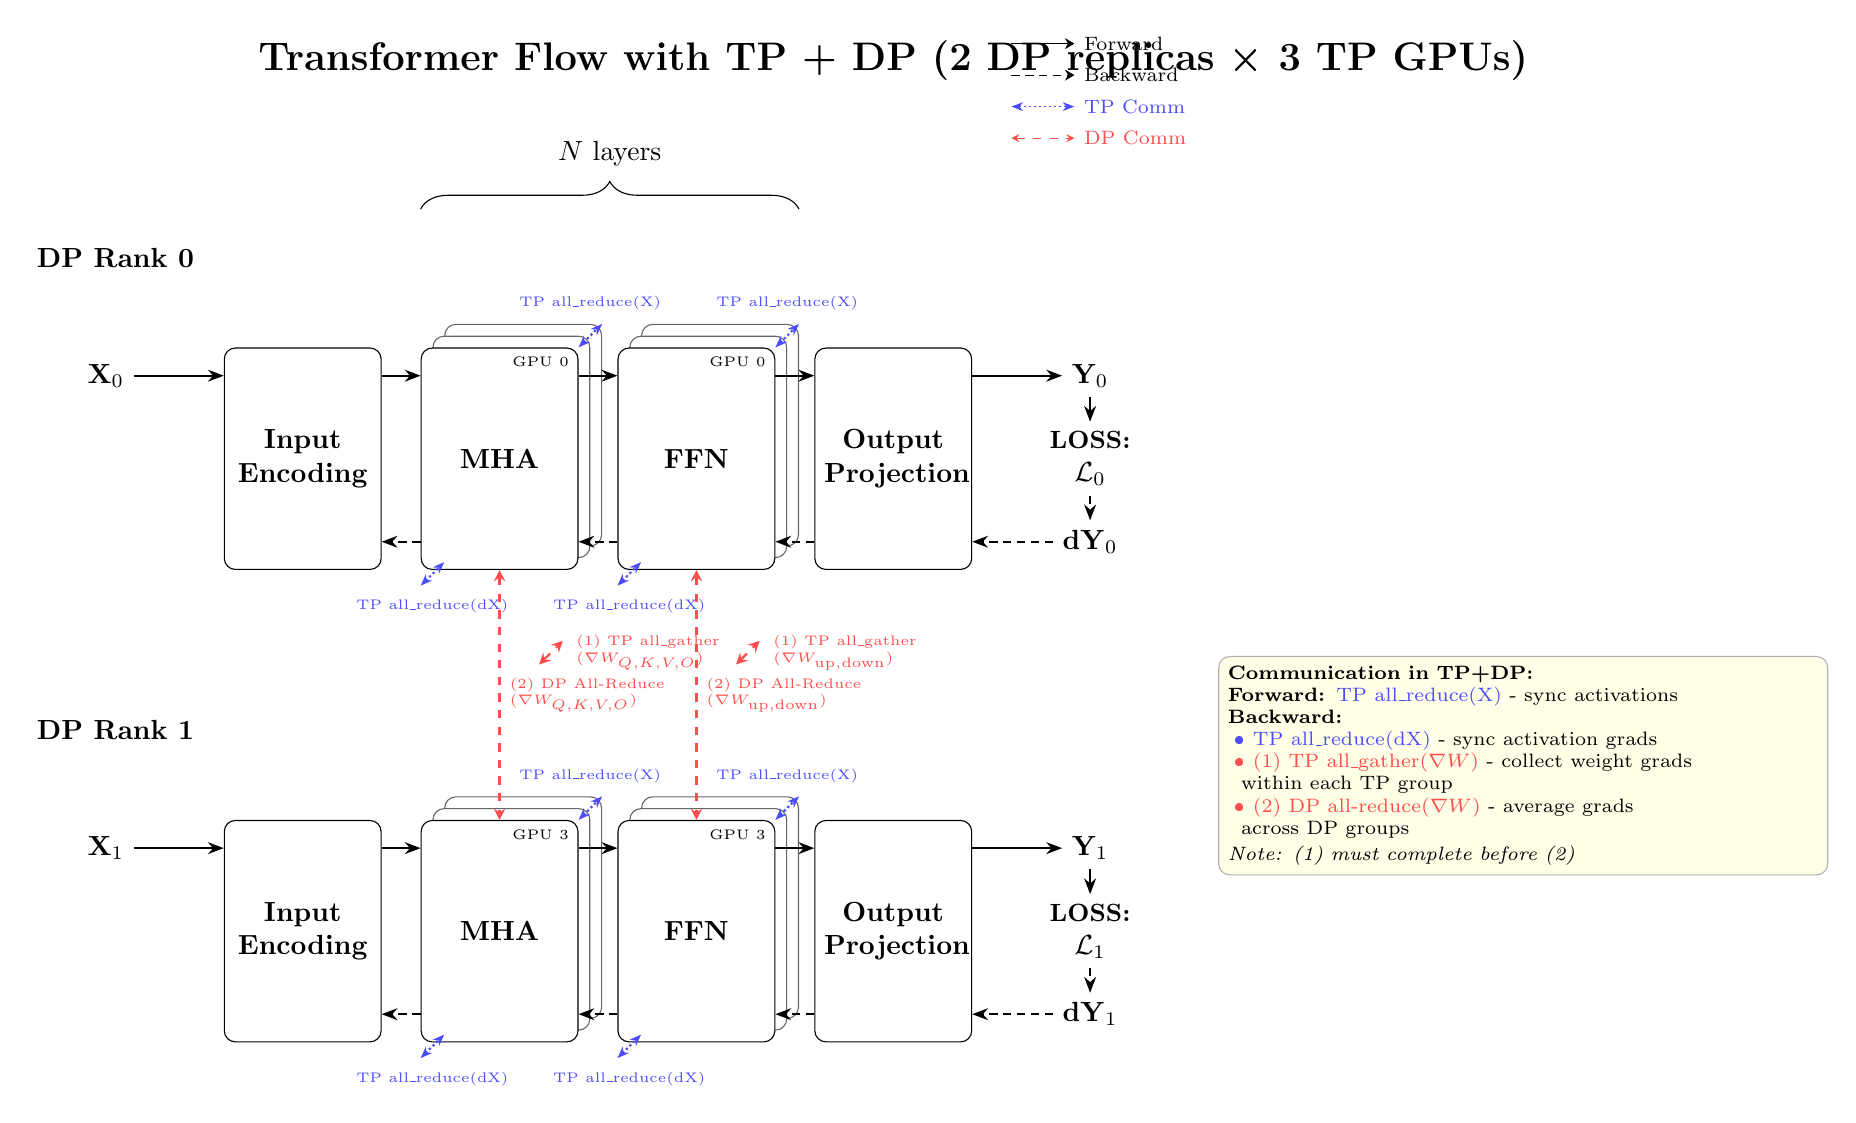
\begin{tikzpicture}[
    node distance=2.5cm,
    >=stealth,
    block/.style={rectangle, draw=black, fill=white, text width=5em, text centered, rounded corners, minimum height=8em, font=\bfseries},
    blockstack/.style={rectangle, draw=black!60, fill=white, text width=5em, text centered, rounded corners, minimum height=8em},
    forward/.style={-{Stealth[length=2mm]}, thick, black},
    backward/.style={-{Stealth[length=2mm]}, thick, black, densely dashed},
    tpcomm/.style={{Stealth[length=1.5mm]}-{Stealth[length=1.5mm]}, thick, blue!70, densely dotted},
    dpcomm/.style={<->, thick, red!70, dashed},
    io/.style={text centered, font=\bfseries}
]
    % Title
    \node[font=\Large\bfseries] at (10, 14) {Transformer Flow with TP + DP (2 DP replicas × 3 TP GPUs)};

    % ========== DP Replica 0 (Upper) ==========
    \node[font=\normalsize\bfseries, anchor=west] at (-1, 11.5) {DP Rank 0};

    \node (input_0) [io] at (0, 10) {$\mathbf{X}_0$};
    \node (encoding_0) [block, right of=input_0, yshift=-3em] {Input\\Encoding};

    % MHA blocks (3 stacked) - TP Group 0
    \node (mha3_0) [blockstack, right of=encoding_0, xshift=0.3cm, yshift=0.3cm] {};
    \node (mha2_0) [blockstack, right of=encoding_0, xshift=0.15cm, yshift=0.15cm] {};
    \node (mha_0) [block, right of=encoding_0] {MHA};
    \node[font=\tiny, anchor=north east] at (mha_0.north east) {GPU 0};

    % FFN blocks (3 stacked) - TP Group 0
    \node (mlp3_0) [blockstack, right of=mha_0, xshift=0.3cm, yshift=0.3cm] {};
    \node (mlp2_0) [blockstack, right of=mha_0, xshift=0.15cm, yshift=0.15cm] {};
    \node (mlp_0) [block, right of=mha_0] {FFN};
    \node[font=\tiny, anchor=north east] at (mlp_0.north east) {GPU 0};

    \node (output_0) [block, right of=mlp_0] {Output\\Projection};
    \node (pred_0) [io, right of=output_0, yshift=3em] {$\mathbf{Y}_0$};
    \node (loss_0) [align=center, io, right of=output_0] {\small LOSS:\\$\mathcal{L}_0$};
    \node (gradient_0) [io, right of=output_0, yshift=-3em] {$\mathbf{dY}_0$};

    % Forward arrows - DP Rank 0
    \draw [forward] (input_0) -- ([yshift=3em]encoding_0.west);
    \draw [forward] ([yshift=3em]encoding_0.east) -- ([yshift=3em]mha_0.west);
    \draw [forward] ([yshift=3em]mha_0.east) -- ([yshift=3em]mlp_0.west);
    \draw [forward] ([yshift=3em]mlp_0.east) -- ([yshift=3em]output_0.west);
    \draw [forward] ([yshift=3em]output_0.east) -- (pred_0);
    \draw [forward] (pred_0) -- (loss_0);
    \draw [backward] (loss_0) -- (gradient_0);

    % Backward arrows - DP Rank 0
    \draw [backward] (gradient_0) -- ([yshift=-3em]output_0.east);
    \draw [backward] ([yshift=-3em]output_0.west) -- ([yshift=-3em]mlp_0.east);
    \draw [backward] ([yshift=-3em]mlp_0.west) -- ([yshift=-3em]mha_0.east);
    \draw [backward] ([yshift=-3em]mha_0.west) -- ([yshift=-3em]encoding_0.east);

    % TP Communications - DP Rank 0
    % Forward All-Reduce
    \draw [tpcomm] (mha_0.north east) -- ([xshift=0.3cm, yshift=0.3cm]mha_0.north east);
    \node[font=\tiny, blue!70, anchor=south] at ([xshift=0.15cm, yshift=0.35cm]mha_0.north east) {TP all\_reduce(X)};

    \draw [tpcomm] (mlp_0.north east) -- ([xshift=0.3cm, yshift=0.3cm]mlp_0.north east);
    \node[font=\tiny, blue!70, anchor=south] at ([xshift=0.15cm, yshift=0.35cm]mlp_0.north east) {TP all\_reduce(X)};

    % Backward All-Reduce - dX
    \draw [tpcomm] ([yshift=-0.2cm]mlp_0.south west) -- ([xshift=0.3cm, yshift=0.1cm]mlp_0.south west);
    \node[font=\tiny, blue!70, anchor=north] at ([xshift=0.15cm, yshift=-0.25cm]mlp_0.south west) {TP all\_reduce(dX)};

    \draw [tpcomm] ([yshift=-0.2cm]mha_0.south west) -- ([xshift=0.3cm, yshift=0.1cm]mha_0.south west);
    \node[font=\tiny, blue!70, anchor=north] at ([xshift=0.15cm, yshift=-0.25cm]mha_0.south west) {TP all\_reduce(dX)};

    % Backward All-Gather for gradients - positioned on right side, before DP all-reduce
    \draw [dpcomm] ([xshift=-0.5cm, yshift=-1.2cm]mlp_0.south east) -- ([xshift=-0.2cm, yshift=-0.9cm]mlp_0.south east);
    \node[font=\tiny, red!70, anchor=west, align=left] at ([xshift=-0.15cm, yshift=-1.05cm]mlp_0.south east) {(1) TP all\_gather\\$(\nabla W_{\text{up},\text{down}})$};

    \draw [dpcomm] ([xshift=-0.5cm, yshift=-1.2cm]mha_0.south east) -- ([xshift=-0.2cm, yshift=-0.9cm]mha_0.south east);
    \node[font=\tiny, red!70, anchor=west, align=left] at ([xshift=-0.15cm, yshift=-1.05cm]mha_0.south east) {(1) TP all\_gather\\$(\nabla W_{Q,K,V,O})$};

    % Brace for layer repetition - DP Rank 0
    \draw[decorate, decoration={brace, amplitude=10pt}]
        ([yshift=5.0em]mha_0.north west) -- ([xshift=0.3cm, yshift=5.0em]mlp_0.north east)
        node[midway, above=12pt, font=\normalsize] {$N$ layers};

    % ========== DP Replica 1 (Lower) ==========
    \node[font=\normalsize\bfseries, anchor=west] at (-1, 5.5) {DP Rank 1};

    \node (input_1) [io] at (0, 4) {$\mathbf{X}_1$};
    \node (encoding_1) [block, right of=input_1, yshift=-3em] {Input\\Encoding};

    % MHA blocks (3 stacked) - TP Group 1
    \node (mha3_1) [blockstack, right of=encoding_1, xshift=0.3cm, yshift=0.3cm] {};
    \node (mha2_1) [blockstack, right of=encoding_1, xshift=0.15cm, yshift=0.15cm] {};
    \node (mha_1) [block, right of=encoding_1] {MHA};
    \node[font=\tiny, anchor=north east] at (mha_1.north east) {GPU 3};

    % FFN blocks (3 stacked) - TP Group 1
    \node (mlp3_1) [blockstack, right of=mha_1, xshift=0.3cm, yshift=0.3cm] {};
    \node (mlp2_1) [blockstack, right of=mha_1, xshift=0.15cm, yshift=0.15cm] {};
    \node (mlp_1) [block, right of=mha_1] {FFN};
    \node[font=\tiny, anchor=north east] at (mlp_1.north east) {GPU 3};

    \node (output_1) [block, right of=mlp_1] {Output\\Projection};
    \node (pred_1) [io, right of=output_1, yshift=3em] {$\mathbf{Y}_1$};
    \node (loss_1) [align=center, io, right of=output_1] {\small LOSS:\\$\mathcal{L}_1$};
    \node (gradient_1) [io, right of=output_1, yshift=-3em] {$\mathbf{dY}_1$};

    % Forward arrows - DP Rank 1
    \draw [forward] (input_1) -- ([yshift=3em]encoding_1.west);
    \draw [forward] ([yshift=3em]encoding_1.east) -- ([yshift=3em]mha_1.west);
    \draw [forward] ([yshift=3em]mha_1.east) -- ([yshift=3em]mlp_1.west);
    \draw [forward] ([yshift=3em]mlp_1.east) -- ([yshift=3em]output_1.west);
    \draw [forward] ([yshift=3em]output_1.east) -- (pred_1);
    \draw [forward] (pred_1) -- (loss_1);
    \draw [backward] (loss_1) -- (gradient_1);

    % Backward arrows - DP Rank 1
    \draw [backward] (gradient_1) -- ([yshift=-3em]output_1.east);
    \draw [backward] ([yshift=-3em]output_1.west) -- ([yshift=-3em]mlp_1.east);
    \draw [backward] ([yshift=-3em]mlp_1.west) -- ([yshift=-3em]mha_1.east);
    \draw [backward] ([yshift=-3em]mha_1.west) -- ([yshift=-3em]encoding_1.east);

    % TP Communications - DP Rank 1
    % Forward All-Reduce
    \draw [tpcomm] (mha_1.north east) -- ([xshift=0.3cm, yshift=0.3cm]mha_1.north east);
    \node[font=\tiny, blue!70, anchor=south] at ([xshift=0.15cm, yshift=0.35cm]mha_1.north east) {TP all\_reduce(X)};

    \draw [tpcomm] (mlp_1.north east) -- ([xshift=0.3cm, yshift=0.3cm]mlp_1.north east);
    \node[font=\tiny, blue!70, anchor=south] at ([xshift=0.15cm, yshift=0.35cm]mlp_1.north east) {TP all\_reduce(X)};

    % Backward All-Reduce - dX
    \draw [tpcomm] ([yshift=-0.2cm]mlp_1.south west) -- ([xshift=0.3cm, yshift=0.1cm]mlp_1.south west);
    \node[font=\tiny, blue!70, anchor=north] at ([xshift=0.15cm, yshift=-0.25cm]mlp_1.south west) {TP all\_reduce(dX)};

    \draw [tpcomm] ([yshift=-0.2cm]mha_1.south west) -- ([xshift=0.3cm, yshift=0.1cm]mha_1.south west);
    \node[font=\tiny, blue!70, anchor=north] at ([xshift=0.15cm, yshift=-0.25cm]mha_1.south west) {TP all\_reduce(dX)};

    % Backward All-Gather for gradients - positioned on right side, before DP all-reduce
    % \draw [dpcomm] ([xshift=0.5cm, yshift=-1.2cm]mlp_1.south east) -- ([xshift=0.8cm, yshift=-0.9cm]mlp_1.south east);
    % \node[font=\tiny, red!70, anchor=west, align=left] at ([xshift=0.85cm, yshift=-1.05cm]mlp_1.south east) {(1) TP all\_gather\\$(\nabla W_{\text{up},\text{down}})$};

    % \draw [dpcomm] ([xshift=0.5cm, yshift=-1.2cm]mha_1.south east) -- ([xshift=0.8cm, yshift=-0.9cm]mha_1.south east);
    % \node[font=\tiny, red!70, anchor=west, align=left] at ([xshift=0.85cm, yshift=-1.05cm]mha_1.south east) {(1) TP all\_gather\\$(\nabla W_{Q,K,V,O})$};

    % ========== DP Communications (Between TP Groups) ==========
    \draw [dpcomm] (mha_0.south) -- (mha_1.north) node[midway, right, font=\tiny, align=left, red!70] {(2) DP All-Reduce\\$(\nabla W_{Q,K,V,O})$};
    \draw [dpcomm] (mlp_0.south) -- (mlp_1.north) node[midway, right, font=\tiny, align=left, red!70] {(2) DP All-Reduce\\$(\nabla W_{\text{up},\text{down}})$};

    % Communication Order Annotation
    \node[font=\scriptsize, align=left, text width=7.5cm, draw=black!30, fill=yellow!10, rounded corners] at ([xshift=15.5cm, yshift=10em]encoding_1.south) {
        \textbf{Communication in TP+DP:}\\
        \textbf{Forward:} \textcolor{blue!70}{TP all\_reduce(X)} - sync activations\\
        \textbf{Backward:}\\
        \hspace{0.3em}\textcolor{blue!70}{• TP all\_reduce(dX)} - sync activation grads\\
        \hspace{0.3em}\textcolor{red!70}{• (1) TP all\_gather($\nabla W$)} - collect weight grads\\
        \hspace{0.6em}within each TP group\\
        \hspace{0.3em}\textcolor{red!70}{• (2) DP all-reduce($\nabla W$)} - average grads\\
        \hspace{0.6em}across DP groups\\[0.2em]
        \textit{Note: (1) must complete before (2)}
    };

    % Labels (Legend)
    \coordinate (legend) at ([xshift=11.5cm, yshift=12em]input_0);

    % Forward
    \draw[forward, -{Stealth[length=1.2mm,width=1.4mm]}, line width=0.3pt] (legend) -- ++(0.8,0)
      node[right, font=\scriptsize] {Forward};

    % Backward
    \draw[backward, -{Stealth[length=1.2mm,width=1.4mm]}, line width=0.3pt] ([yshift=-0.4cm]legend) -- ++(0.8,0)
      node[right, font=\scriptsize] {Backward};

    % TP Comm
    \draw[tpcomm, line width=0.3pt] ([yshift=-0.8cm]legend) -- ++(0.8,0)
      node[right, font=\scriptsize] {TP Comm};

    % DP Comm
    \draw[dpcomm, line width=0.3pt] ([yshift=-1.2cm]legend) -- ++(0.8,0)
      node[right, font=\scriptsize] {DP Comm};

\end{tikzpicture}%
}
  \caption{Overall Transformer layer with combined data and tensor
  parallelism. Horizontally, each tensor-parallel group of size $N_T$
  jointly implements a sharded version of the layer (as in
  Section~\ref{sec:tp}). Vertically, $N_D$ such groups form a data-parallel grid:
  each row processes a different mini-batch shard, and gradients are
  synchronized across rows. All-Reduce and All-Gather collectives are
  annotated where they appear.}
  \label{fig:dp_tp_overall_flow}
\end{figure}

% ------------------------ 8.2 From Single-Node to TP to DP+TP --------
\subsection{From Single-Node to TP to DP+TP}

It is useful to view DP+TP as a sequence of incremental modifications to
the single-node computation of Section~\ref{sec:sn}:

\paragraph{Single node (Section~\ref{sec:sn}).}
All parameters and activations live on a single device. Each linear layer
is a single matmul, and no collectives are needed.

\paragraph{Tensor parallelism only (Section~\ref{sec:tp}).}
We split large matrices across $N_T$ devices:

\begin{itemize}
  \item \textbf{Column-parallel} linears:
        weights are split along the output dimension. Each shard computes
        a slice of the output; later operations either keep that sharded
        representation or perform an All-Gather to reconstruct the full
        tensor.
  \item \textbf{Row-parallel} linears:
        weights and inputs are split along the input dimension. Each shard
        computes a partial result, and an All-Reduce is used to sum
        partial outputs.
\end{itemize}

Within a single TP group, all devices see the same batch and activations
are sharded along feature dimensions. Collectives (All-Reduce and possibly
All-Gather) appear \emph{inside} the layer graphs.

\paragraph{Data parallelism only (Section~\ref{sec:dp}).}
We keep the single-node graphs intact but replicate them across $N_D$
devices, each with a different mini-batch shard. The only collective is
an All-Reduce over parameter gradients at the end of the backward pass.

\paragraph{Combining DP and TP.}
In DP+TP we apply both modifications at once:

\begin{itemize}
  \item Each data-parallel replica is itself a TP group of $N_T$ devices.
        Inside that group, all TP sharding and collectives from
        Section~\ref{sec:tp} apply as-is.
  \item Across data-parallel replicas, we perform gradient All-Reduces as
        in Section~\ref{sec:dp}, now applied to \emph{sharded} parameters (the TP
        shards of each weight matrix).
\end{itemize}

Thus, the internal structure of each MHA/MLP/output block on a \emph{per
shard} basis is unchanged; the only differences lie in how many devices
share each tensor and which collectives connect them.

% ------------------------ 8.3 Forward Pass under DP+TP ---------------
\subsection{Forward Pass under DP+TP}

From the perspective of a single TP shard inside DP+TP, the forward pass
is the same as in the TP-only model (Section~\ref{sec:tp}):

\begin{itemize}
  \item the input is the local mini-batch shard $\mathbf{X}_d$ of shape
        $[B_{\text{local}}, S, D]$;
  \item column-parallel and row-parallel linears are applied as before;
  \item intermediate activations (e.g., per-head Q/K/V, intermediate MLP
        features) are sharded across the $N_T$ devices.
\end{itemize}

The main new ingredient is the use of \textbf{All-Gather} on activations
in certain places where a subsequent operation requires the full (unsharded)
tensor.

Common examples include:

\begin{itemize}
  \item \textbf{Vocabulary-parallel output projection.}
        If the final LM head weight $\mathbf{W}_{\text{lm}}$ is sharded
        across TP devices along the vocabulary dimension, each shard
        produces logits for a subset of the vocabulary. To compute the
        softmax and loss with the full vocabulary on each device, we
        perform an All-Gather of the partial logits slices to assemble the
        full $[B_{\text{local}}, S, V]$ tensor.
  \item \textbf{Embedding layers.}
        Similarly, if the token embedding matrix is sharded along the
        vocabulary dimension, embedding lookups may produce sharded
        embeddings that must be All-Gathered before being passed into a
        subsequent layer that expects an unsharded $[B_{\text{local}}, S,
        D]$ representation.
  \item \textbf{Non-sharded operations.}
        Any operation that conceptually acts on the full hidden dimension
        (e.g., a global normalization or a non-sharded residual branch)
        may require an All-Gather of the sharded activations before it can
        be applied, unless the model has been carefully arranged so that
        all such operations either run locally on shards or are replaced
        by TP-friendly variants.
\end{itemize}

All-Reduce and All-Gather thus play complementary roles inside a TP group:

\begin{itemize}
  \item \textbf{All-Reduce} combines partial results that were computed on
        a sharded input (row-parallel linears, sharded gradients).
  \item \textbf{All-Gather} reassembles tensor slices that were produced
        by column-parallel linears or vocabulary-parallel projections
        when the next operation needs the full tensor.
\end{itemize}

Data parallelism does not change these intra-group collectives; it only
changes which mini-batch $\mathbf{X}_d$ is fed into the TP group.

% ------------------------ 8.4 Backward Pass and Gradient Sync --------
\subsection{Backward Pass and Gradient Synchronization}

In DP+TP, the backward pass combines:

\begin{itemize}
  \item the TP-only backward graphs from Section~\ref{sec:tp}, including all
        intra-group All-Reduce and All-Gather operations on activations
        and partial gradients, and
  \item the DP-only gradient synchronization from Section~\ref{sec:dp}, now applied
        to the sharded parameters of each TP group.
\end{itemize}

Concretely, for a given parameter tensor $W$:

\begin{itemize}
  \item In TP-only:
    \begin{itemize}
      \item $W$ is split into shards $W^{(t)}$ over $t=0,\dots,N_T-1$,
            each stored on a different device inside a TP group.
      \item Backward through the local matmul yields a local gradient
            $\nabla W^{(t)}$ on each shard.
      \item If $W$ appears in a row-parallel configuration, partial
            gradients w.r.t.\ inputs are All-Reduced across $t$.
    \end{itemize}
  \item In DP+TP:
    \begin{itemize}
      \item The above TP logic is applied independently within each DP
            replica $d$, yielding $\nabla W^{(t,d)}$ on shard $t$ in
            replica $d$.
      \item \emph{Across} replicas, we perform an All-Reduce over $d$ for
            each shard $t$:
            \[
              \nabla W^{(t)}
                = \frac{1}{N_D}
                  \sum_{d=0}^{N_D-1} \nabla W^{(t,d)}.
            \]
            This is a data-parallel gradient synchronization, but now
            replicated over all TP shards in parallel.
    \end{itemize}
\end{itemize}

Thus, every parameter shard participates in two types of collectives:

\begin{itemize}
  \item \textbf{TP collectives} inside a DP replica:
        All-Reduce/All-Gather across $t$ (row-/column-parallel logic).
  \item \textbf{DP collectives} across replicas:
        All-Reduce across $d$ for each shard index $t$.
\end{itemize}

The combination ensures that, at the end of the backward pass, all TP
groups in all DP replicas hold identical, properly aggregated gradients
for their local shards $W^{(t)}$, so that the optimizer update is
consistent across the entire system.

% ------------------------ 8.5 Communication Summary ------------------
\subsection{Communication Summary and Differences from TP-only / DP-only}

We summarize the main differences compared to TP-only (Section~\ref{sec:tp}) and
DP-only (Section~\ref{sec:dp}):

\paragraph{Compared to TP-only.}

\begin{itemize}
  \item \textbf{Same per-layer sharding.}
        Inside one TP group, the forward/backward graphs, the placement of
        All-Reduce and All-Gather, and the tensor shapes are identical to
        the TP-only case.
  \item \textbf{Additional gradient All-Reduce over DP replicas.}
        Every parameter shard now participates in an extra All-Reduce over
        the DP dimension to average gradients across mini-batch shards.
  \item \textbf{No change in local activations.}
        Activation memory and compute patterns inside a TP group do not
        change when DP is added; DP only affects which samples are seen by
        each replica and how parameter gradients are combined.
\end{itemize}

\paragraph{Compared to DP-only.}

\begin{itemize}
  \item \textbf{Sharded model within each replica.}
        Instead of a full copy of the model per DP replica, each replica
        contains a TP-sharded model: parameters and some activations are
        split across $N_T$ devices.
  \item \textbf{More frequent collectives.}
        DP-only uses All-Reduce once per step per parameter tensor. In
        DP+TP, we additionally have intra-replica All-Reduce/All-Gather
        operations inside most layers (MHA, MLP, embeddings, LM head).
  \item \textbf{Per-device memory and compute.}
        TP reduces per-device parameter and activation memory by
        approximately $1/N_T$, at the cost of extra intra-layer
        communication. DP further reduces per-device activation memory by
        a factor of $1/N_D$ by splitting the batch.
\end{itemize}

Overall, DP+TP can be seen as:

\begin{quote}
  “Take the TP-sharded Transformer layer of Section~\ref{sec:tp}, run it on different
  mini-batch shards as in Section~\ref{sec:dp}, and add one more All-Reduce per
  parameter shard to average gradients across replicas.”
\end{quote}

All-Gather operations appear wherever TP has produced sharded activations
that must be globally visible (e.g., logits over the full vocabulary),
while All-Reduce is used both to combine partial TP results and to
aggregate gradients across data-parallel replicas.

\fi
\clearpage

% ==========================================================
% 9. Summary and Practical Takeaways
% ==========================================================
\ifkorean
  % ==========================================================
% 9. 요약과 실용적인 정리
% ==========================================================
\section{요약과 실용적인 정리}

이 장에서는 앞선 장들에서 다룬 핵심 아이디어를 정리하고,
트랜스포머 학습이 실제 하드웨어에서 어떻게 수행되는지에 대한
실용적인 질문들과 연결한다.
새로운 표기법을 도입하기보다는,
실행 다이어그램을 읽거나 연산 비용을 추정하거나
모델 병렬화 방식을 결정할 때 유용한
몇 가지 사고 모형(mental model)에 초점을 맞춘다.

\subsection{기울기에서 그래프, 그리고 트랜스포머로}

이 문서의 앞부분에서는 세 가지 층위의 직관을 쌓아 왔다.

\begin{itemize}
  \item \textbf{선형 변환으로서의 기울기.}
        한 레이어를 통과하는 역전파는,
        또 다른 계산 그래프로 볼 수 있다.
        여기서 각 순전파 연산은 하나 이상의 역전파 연산
        (보통 전치된 matmul 등)을 기여한다.
        이 관점은 다음과 같은 간단한 경험 법칙으로 이어진다:
        \emph{선형 레이어 하나는 역전파에서
        대략 순전파의 두 배 비용을 유발한다.}
  \item \textbf{그래프 표기 규칙.}
        순전파 텐서, 기울기, 파라미터는
        명시적인 차원(shape) 라벨을 가진 노드로 표현된다.
        화살표와 라벨을 통해, 코드를 보지 않고도
        각 단계에서 어떤 matmul과 원소별 연산이 일어나는지
        읽어낼 수 있다.
  \item \textbf{단일 노드 트랜스포머.}
        하나의 트랜스포머 레이어는 다음 구성 요소들의 합성일 뿐이다.
        \begin{itemize}
          \item 임베딩 lookup + 위치 인코딩,
          \item MHA (레이어 정규화, Q/K/V 프로젝션,
                어텐션, 출력 프로젝션, 잔차 연결),
          \item MLP (레이어 정규화, 상향 프로젝션,
                비선형 활성 함수, 하향 프로젝션, 잔차 연결),
          \item 출력 프로젝션 + 소프트맥스 + 손실.
        \end{itemize}
        각 블록에는 순전파 그래프가 있고,
        이에 정확히 대응하는 역전파 그래프가 존재하는데,
        순전파의 각 matmul마다 역전파에서
        한두 개의 matmul이 짝을 이룬다.
\end{itemize}

Section~\ref{sec:sn}의 단일 노드 다이어그램은
이후에 등장하는 모든 병렬 변형의 “기본 케이스(base case)”다.
어떤 병렬 실행 구성도, 결국은
이 동일한 기반 계산 그래프를 쪼개고(split), 복제하고(replicate),
다시 이어 붙이는(reconnect) 방법이라고 볼 수 있다.

\subsection{연산량과 메모리: 무엇이 중요한가}

모든 레이어를 관통해 나타나는 공통적인 패턴들은 다음과 같다.

\begin{itemize}
  \item \textbf{matmul이 지배적이다.}
        대부분의 FLOPs는 선형 레이어에 들어 있다
        (Q/K/V 프로젝션, 어텐션 출력 프로젝션,
        MLP 상향/하향 프로젝션, 최종 출력 프로젝션).
        elementwise 연산(softmax, GELU, layernorm 등)은
        정확도와 안정성에는 중요하지만,
        연산량 측면에서는 상대적으로 저렴하다.
  \item \textbf{matmul의 역전파 비용은 대략 순전파의 두 배.}
        순전파의 matmul $XW$ 하나는 최소한 다음 두 개를 만든다.
        \begin{itemize}
          \item 입력 $X$로 기울기를 전파하기 위한 역전파 matmul 하나,
          \item 가중치 $W$에 기울기를 누적하기 위한 역전파 matmul 하나.
        \end{itemize}
        이는 MHA와 MLP에 대한 역전파 다이어그램에서
        명시적으로 확인할 수 있다.
  \item \textbf{어텐션과 MLP가 주된 비용원.}
        다중 헤드 어텐션의 Q/K/V 프로젝션과
        출력 프로젝션, 그리고 MLP의 상향/하향 프로젝션이
        대부분의 FLOPs를 차지한다.
        레이어 정규화와 잔차 연결, 활성 함수 등은
        상대적으로 저렴하다.
  \item \textbf{잔차 연결은 비용을 크게 늘리지 않는다.}
        잔차는 기울기 경로를 분기시키긴 하지만,
        점근적인 복잡도를 바꾸지는 않는다.
        잔차 add는 순전파·역전파 모두에서
        가벼운 elementwise 연산만 추가한다.
  \item \textbf{레이어 정규화는 항상 있지만, 비용은 상대적으로 작다.}
        레이어 정규화는 토큰당 약간의 연산과
        소량의 파라미터를 추가한다.
        역전파는 ReLU 같은 단순 활성 함수보다 조금 복잡하지만,
        여전히 주변의 큰 matmul들에 비하면 훨씬 저렴하다.
\end{itemize}

따라서 모델의 비용을 대략적으로 추정할 때는,
큰 matmul들의 개수만 세고,
해당 층들에 대해서는 역전파가
순전파의 약 두 배 비용이 든다고 기억하는 것만으로도
충분한 경우가 많다.

\subsection{단일 노드, TP, DP, DP+TP 비교}

뒤쪽 장들에서는 네 가지 실행 모드를 비교했다.

\begin{itemize}
  \item \textbf{단일 노드 (Section~\ref{sec:sn}).}
        모든 파라미터와 활성값이 하나의 디바이스에 존재한다.
        이 장의 다이어그램은 참조 구현에 해당한다:
        샤딩도 없고 집합 통신도 없으며,
        단지 matmul과 elementwise 연산이 차례대로 수행될 뿐이다.
  \item \textbf{텐서 병렬화 (Section~\ref{sec:tp}).}
        가중치 행렬과 일부 활성값을
        \emph{모델 샤드(model shard)} 내부의 $N_T$개 디바이스에 나누어 저장한다.
        컬럼 병렬/로우 병렬 선형 레이어가
        단일 노드의 matmul을 대체한다.
        부분 결과를 합치거나(shard 합산),
        샤딩된 텐서를 다시 조립하기 위해,
        레이어 그래프 \emph{내부에} All-Reduce와 All-Gather가 등장한다.
  \item \textbf{데이터 병렬화 (Section~\ref{sec:dp}).}
        전체 모델(또는 전체 TP 샤드)을 $N_D$ 디바이스에 복제한다.
        각 복제본은 서로 다른 미니배치 조각을 보고,
        단일 노드 또는 TP 설정에서와 동일한
        순전파/역전파 그래프를 실행한다.
        새롭게 등장하는 집합 통신은,
        역전파 마지막에 파라미터 기울기에 대해 수행하는
        All-Reduce 한 번뿐이다.
  \item \textbf{DP + TP (Section~\ref{sec:dp_tp}).}
        각 데이터 병렬 복제본 자체가 하나의 TP 그룹이다.
        TP 그룹 내부에서는 Section~\ref{sec:tp}에서 설명한
        레이어 내부 집합 통신(All-Reduce, All-Gather)이 그대로 적용된다.
        복제본들 사이에서는 각 TP 샤드에 대한 기울기를 평균 내기 위해
        추가적인 All-Reduce를 수행한다.
        일부 레이어(예: vocabulary-parallel 출력 헤드)는,
        이후 연산이 전체(샤딩되지 않은) 텐서를 필요로 할 때
        활성값에 대한 All-Gather를 요구한다.
\end{itemize}

즉, 다음과 같이 요약할 수 있다.

\begin{center}
\begin{tabular}{ll}
\textbf{Single node} & 집합 통신 없음, 전체 가중치가 한 디바이스에 존재 \\[0.2em]
\textbf{TP}          & 가중치/활성값 샤딩, 레이어 내부 집합 통신 \\[0.2em]
\textbf{DP}          & 모델 복제, 기울기 All-Reduce만 수행 \\[0.2em]
\textbf{DP+TP}       & 각 복제본 안에서 TP + 복제본 간 기울기 All-Reduce
\end{tabular}
\end{center}

개념적으로 이들 모드 중 어느 것도
트랜스포머가 \emph{무엇을} 계산하는지를 바꾸지는 않는다.
단지, 그래프의 각 조각이 어느 디바이스에서 실행되는지와
부분 결과들이 어떻게 다시 이어 붙는지가 달라질 뿐이다.

\subsection{도식 읽는 방법과 활용}

이 문서 전반의 다이어그램들은 반복적으로 마주치는
몇 가지 질문에 답하도록 설계되었다.

\begin{itemize}
  \item \textbf{큰 matmul은 어디에 있는가?}
        $[B,S,D]$와 같은 모양의 활성 텐서와,
        $[D,D_{\text{ff}}]$, $[D,D]$, $[D,D_{\text{vocab}}]$ 형태의
        가중치 행렬을 연결하는 직사각형 노드를 찾아보라.
        이들이 FLOPs의 주된 원천이다.
  \item \textbf{기울기는 어디로 흐르는가?}
        점선 화살표와 역전파 전용 노드들은
        $\mathrm{d}\mathcal{L}$이 어떻게 전파되는지 보여 준다.
        이 화살표를 따라가다 보면,
        어떤 텐서를 역전파를 위해 저장해야 하는지,
        그리고 어디서 활성값을 다시 계산할 수 있는지가 드러난다.
  \item \textbf{메모리는 어디에서 쓰이는가?}
        순전파 텐서가 역전파에서 다시 필요해지는 지점은
        모두 활성값 메모리에 기여한다.
        특히 어텐션 스코어 텐서 $[B,N_H,S,S]$와
        MLP 중간 텐서 $[B,S,D_{\text{ff}}]$는
        메모리 사용량이 크다.
  \item \textbf{집합 통신은 어디에서 발생하는가?}
        TP/DP 다이어그램에서는 색깔이 있는 화살표나
        라벨이 붙은 화살표가 All-Reduce/All-Gather를 나타낸다.
        이 위치들이 많은 디바이스로 확장할 때의
        통신 비용과 크리티컬 패스 길이를 결정한다.
\end{itemize}

이러한 “어휘”에 익숙해지면,
새로운 아키텍처(예: 변형된 MLP, 다른 어텐션 메커니즘)를 보았을 때도
그 핵심적인 연산 비용과 병렬화 패턴을
곧바로 스케치할 수 있게 된다.

\subsection{실용적인 규칙 정리}

다음의 비공식적인 규칙들은
앞선 장들에서의 실용적인 교훈들을 간단히 요약한 것이다.

\begin{itemize}
  \item \textbf{항상 단일 노드 그래프에서 시작하라.}
        추론을 시작할 때는 언제나 가장 단순한 관점에서 출발하라:
        이 모델이 단일 디바이스에서 실행된다면
        무엇을 어떻게 할 것인가?
        그다음 TP와 DP를 그 위에 겹쳐서 생각한다.
  \item \textbf{코드 줄 수가 아니라 matmul 개수로 생각하라.}
        토큰당 등장하는 큰 matmul이 몇 개인지 세고,
        그 각각에 대해 역전파에서
        (대략 두 배) 추가 비용을 지불해야 한다는 사실을 기억하라.
  \item \textbf{TP는 메모리를 줄이는 대신, 레이어 내부 통신을 추가한다.}
        피처 차원 방향으로 샤딩하면
        디바이스당 메모리는 줄어들지만,
        레이어 내부에 All-Reduce/All-Gather가 생긴다.
        모델이 단일 디바이스 메모리에 들어가지 않을 때
        사용하는 수단이다.
  \item \textbf{DP는 전역 배치 크기를 늘리는 대신, 기울기 통신을 추가한다.}
        모델을 복제하는 방식은 단순하고
        레이어 그래프를 그대로 유지하지만,
        모든 파라미터가 기울기 All-Reduce에 참여해야 한다.
  \item \textbf{아주 큰 모델에서는 보통 DP + TP가 기본값이다.}
        실제 대규모 시스템에서는 TP로 모델을 “맞추고”,
        DP로 배치와 처리량을 확장하는 조합이 일반적이다.
  \item \textbf{스케일링 한계는 집합 통신이 정한다.}
        모델이 메모리에 들어간 이후에는,
        추가적인 속도 향상은 거의
        All-Reduce/All-Gather의 개수, 크기, 위치에 의해 제한된다.
\end{itemize}

\subsection{다음 단계}

이 문서는 의도적으로 하나의 트랜스포머 레이어와
소수의 병렬화 전략에 집중했다.
실제 시스템에서의 확장은 다음과 같은 기법들을 포함한다.

\begin{itemize}
  \item \textbf{파이프라인 병렬화(pipeline parallelism):}
        레이어들을 깊이 방향으로 디바이스에 나누고,
        마이크로 배치를 중첩(overlap)시키는 방식.
  \item \textbf{활성값 체크포인팅(activation checkpointing):}
        활성값 메모리를 줄이는 대신,
        역전파 시 일부 순전파를 재계산하는 방식.
  \item \textbf{옵티마이저/파라미터 샤딩:}
        옵티마이저 상태와 심지어 파라미터 자체를
        노드들에 더 복잡한 방식으로 분산(shard)하는 기법들.
\end{itemize}

그러나 핵심 사고 모형은 그대로다.
먼저 단일 노드 다이어그램처럼
정확한 계산 그래프를 세운 뒤,
다음 세 가지 질문을 던진다:
이 그래프가 디바이스들 사이에 어떻게 잘리는가,
통신은 어디에 나타나는가,
그리고 기울기는 어떻게 집계되는가.
이 세 가지가 명확하다면,
겉보기에는 복잡해 보이는 대부분의 병렬 구성도
익숙한 기본 블록들로 환원해 이해할 수 있다.

\else
  % ==========================================================
% 9. Summary and Practical Takeaways
% ==========================================================
\section{Summary and Practical Takeaways}

This chapter summarizes the main ideas of the previous sections and
connects them to practical questions about how Transformer training
actually runs on hardware. Rather than introducing new notation, we focus
on a small number of mental models that are useful when reading execution
diagrams, reasoning about cost, or deciding how to parallelize a model.

\subsection{From Gradients to Graphs to Transformers}

The early chapters of this document built up three layers of intuition:

\begin{itemize}
  \item \textbf{Gradients as linear maps.}
        Backpropagation through a layer can be viewed as another
        computation graph, where each forward operation contributes one or
        more backward operations (often transposed matmuls). This leads to
        the simple rule of thumb that a linear layer roughly doubles the
        cost in the backward pass.
  \item \textbf{Graph conventions.}
        Forward tensors, gradients, and parameters are represented as
        nodes with explicit shapes. Arrows and labels make it possible to
        read off which matmuls and elementwise ops appear in each phase
        without looking at code.
  \item \textbf{Single-node Transformer.}
        A Transformer layer is just a composition of:
        \begin{itemize}
          \item embedding lookup + positional encoding,
          \item MHA (LN, QKV projections, attention, output projection,
                residual),
          \item MLP (LN, up-projection, non-linearity, down-projection,
                residual),
          \item output projection + softmax + loss.
        \end{itemize}
        Each block has a forward graph and a matching backward graph with
        one or two matmuls for each forward matmul.
\end{itemize}

The single-node diagrams in Section~\ref{sec:sn} are therefore the ``base case'' for
all later parallel variants: every parallel configuration is just a way of
splitting, replicating, and reconnecting this same underlying graph.

\subsection{Cost and Memory: What Really Matters}

Several general patterns show up across all layers:

\begin{itemize}
  \item \textbf{Matmuls dominate.}
        The vast majority of FLOPs live in linear layers
        (Q/K/V projections, attention output projection, MLP up/down
        projections, output projection). Elementwise ops (softmax, GELU,
        layernorm) are important for correctness but cheap by comparison.
  \item \textbf{Backward is $\approx 2\times$ forward for matmuls.}
        Each forward matmul $XW$ produces at least:
        \begin{itemize}
          \item one backward matmul to propagate gradients to $X$, and
          \item one backward matmul to accumulate gradients into $W$.
        \end{itemize}
        This is explicitly visible in the backward diagrams for MHA and
        MLP.
  \item \textbf{Residual connections do not add much cost.}
        They split gradients but do not change asymptotic complexity:
        a residual add introduces cheap elementwise ops in both directions.
  \item \textbf{Layer normalization is modest but ubiquitous.}
        LN adds some per-token compute and a small number of parameters.
        Its backward pass is a bit more involved than, say, ReLU, but
        still far cheaper than the surrounding matmuls.
\end{itemize}

When approximating the cost of a model, it is therefore usually enough to
count the large matmuls and remember that the backward pass is roughly
twice as expensive as the forward pass for those layers.

\subsection{Single-Node vs.\ TP vs.\ DP vs.\ DP+TP}

The later chapters compared four execution modes:

\begin{itemize}
  \item \textbf{Single node (Section~\ref{sec:sn}).}
        All parameters and activations live on one device. The diagrams in
        that section are the reference implementation: no sharding, no
        collectives, just a sequence of matmuls and elementwise ops.
  \item \textbf{Tensor parallelism (Section~\ref{sec:tp}).}
        Weight matrices and some activations are split across $N_T$
        devices inside a \emph{model shard}. Column-parallel and
        row-parallel linears replace the single-node matmuls. All-Reduce
        and All-Gather collectives appear \emph{inside} the layer graphs
        to combine partial results or reassemble sharded tensors.
  \item \textbf{Data parallelism (Section~\ref{sec:dp}).}
        The full model (or full TP shard) is replicated across $N_D$
        devices. Each replica sees a different mini-batch shard and runs
        the same forward/backward graph as in the single-node or TP case.
        The only new collective is an All-Reduce over parameter gradients
        at the end of the backward pass.
  \item \textbf{DP + TP (Section~\ref{sec:dp_tp}).}
        Each DP replica is itself a TP group. Inside a TP group, all
        intra-layer collectives from Section~\ref{sec:tp} (All-Reduce, All-Gather)
        still apply. Across replicas, additional All-Reduces average
        gradients for each TP shard. Some layers (e.g., vocabulary-parallel
        output heads) require All-Gather on activations when a subsequent
        operation needs a full (unsharded) tensor.
\end{itemize}

In other words:

\begin{center}
\begin{tabular}{ll}
\textbf{Single node} & no collectives, full weights on one device \\[0.2em]
\textbf{TP}          & shard weights/activations, intra-layer collectives \\[0.2em]
\textbf{DP}          & replicate model, gradient All-Reduce only \\[0.2em]
\textbf{DP+TP}       & TP inside each replica + DP gradient All-Reduce
\end{tabular}
\end{center}

Conceptually, none of these modes change what the Transformer \emph{is}
computing; they only change where each piece of the graph runs and how
partial results are stitched back together.

\subsection{Reading and Using the Diagrams}

The diagrams throughout this document are designed to answer a small set
of recurring questions:

\begin{itemize}
  \item \textbf{Where are the big matmuls?}
        Look for rectangular nodes with shapes like $[B,S,D]$ and weight
        matrices with shapes $[D,D_{\text{ff}}]$, $[D,D]$, or
        $[D,D_{\text{vocab}}]$. These are the main sources of FLOPs.
  \item \textbf{Where do gradients flow?}
        Dashed arrows and backward-specific nodes show how
        $\mathrm{d}\mathcal{L}$ propagates. Following these arrows makes
        it clear which tensors need to be stored for backward and where
        activations can be recomputed.
  \item \textbf{Where is memory used?}
        Any place where a forward tensor is needed again in backward
        contributes to activation memory. Attention score tensors
        $[B,N_H,S,S]$ and intermediate MLP activations $[B,S,D_{\text{ff}}]$
        are particularly expensive.
  \item \textbf{Where do collectives occur?}
        In TP and DP diagrams, colored or labeled arrows denote All-Reduce
        and All-Gather. These positions determine the communication cost
        and the critical path length when scaling to many devices.
\end{itemize}

With this vocabulary, one can often look at a new architecture (e.g., a
variant MLP, a different attention mechanism) and immediately sketch its
core cost and parallelization pattern.

\subsection{Practical Rules of Thumb}

The following informal rules capture many of the practical lessons from
the previous chapters:

\begin{itemize}
  \item \textbf{Start with the single-node graph.}
        Always begin reasoning from the simplest view: what would the
        model do on a single device? Then layer TP and DP on top.
  \item \textbf{Think in matmuls, not lines of code.}
        Count how many large matmuls appear per token, and remember that
        each will be paid for again (roughly twice) in backward.
  \item \textbf{TP trades memory for intra-layer communication.}
        Sharding along feature dimensions reduces per-device memory but
        introduces All-Reduce/All-Gather inside layers. Use it when the
        model is too large for a single device.
  \item \textbf{DP trades global batch size for gradient communication.}
        Replicating the model is simple and keeps layer graphs intact,
        but every parameter must participate in a gradient All-Reduce.
  \item \textbf{DP + TP is the default for very large models.}
        In practice, most large-scale systems combine both: TP to make the
        model fit, DP to scale the batch and throughput.
  \item \textbf{Collectives define your scaling limits.}
        Once the model fits in memory, additional speedups are mostly
        limited by the number, size, and placement of All-Reduce and
        All-Gather operations.
\end{itemize}

\subsection{Where to Go Next}

This document deliberately focused on a single Transformer layer and a
small set of parallel strategies. Extensions in real systems include:

\begin{itemize}
  \item \textbf{Pipeline parallelism:} splitting layers across devices in
        depth and overlapping micro-batches.
  \item \textbf{Activation checkpointing:} trading recomputation for
        reduced activation memory.
  \item \textbf{Optimizer and parameter sharding:} partitioning optimizer
        state and even the parameters themselves across nodes in more
        complex ways.
\end{itemize}

However, the core mental model remains the same: start from a precise
computation graph (as in the single-node diagrams), then ask how that
graph is sliced across devices, where communication appears, and how
gradients are aggregated. If those three questions are clear, most
seemingly complicated parallel configurations reduce to simple, familiar
building blocks.

\fi

\end{document}
